\documentclass[a4paper]{book}

\usepackage[left=3.81cm, right=2.54cm, top=2.54cm, bottom=3.17cm]{geometry}
\usepackage[T1]{fontenc} 
\usepackage[latin1]{inputenc} % latin1 char encoding
\usepackage[spanish]{babel}
\usepackage{amssymb}
\usepackage{amsmath}
\usepackage{amsthm} % theorems
\usepackage{enumerate}
\usepackage{epsfig}
\usepackage{multirow}

\usepackage{graphicx}
\usepackage{tikz}
\usetikzlibrary{shapes,arrows,automata,positioning,fit}

\usepackage{url}
\usepackage{verbatim}
\usepackage{array}
\usepackage{algorithm}
\usepackage{algorithmic}

\usepackage{fixme}
\usepackage{xspace}
\usepackage{ifthen}

\usepackage{pdfpages}
\selectlanguage{spanish}
\usepackage[utf8]{inputenc}

\renewcommand{\listtablename}{Indice de Tablas}
\renewcommand{\tablename}{Tabla}

% Sin sangria
%\parindent=0mm  

% Espacio entre parrafos
%\parskip=4mm

% Dialogue template
\newenvironment{dialogue}%
   {\begin{it}%
    \begin{list}{}%
         {\setlength{\leftmargin}{.3cm}}%
         \item[]}%
   {\end{list}%
    \end{it}}

\begin{document}

% PARTE PRELIMINAR
\frontmatter % Numeros de paginas con numeros romanos

\thispagestyle{empty}

\begin{titlepage}
\begin{center}

{ \vspace*{1cm} }
\huge{\textsc{\textmd{Universidad Nacional de C\'ordoba}}}\\[1cm]
\Large{\textsc{\textmd{Facultad de Matem\'atica, Astronom\'ia, F\'isica y Computaci\'on}}}\\[1cm]


\includegraphics[scale=0.1]{unc.jpg}
\Large{Trabajo final del Doctorado en Ciencias de la Computaci\'on}\\[1cm]

\LARGE{\textbf{Generaci\'on de expresiones referenciales: un punto de vista l\'ogico-humano }}\\[2cm]


\Large{Alumna: Ivana Romina Altamirano}\\[1.3cm]

\Large{Supervisora: Luciana Benotti}

\vfill
\vfill
%\large{C�RDOBA} \hfill \large{ARGENTINA}\\[2cm]

\large{C�RDOBA } \large{ARGENTINA}\\ 
\large{Febrero, 2016} 


\end{center}
\end{titlepage}

%{ \vspace*{1cm} }

\Large{\textsc{P\'agina para los evaluadores}}\\[3cm]

\large{Calificaci\'on:}\\[1.8cm]

\large{Comentarios:}\\[5cm]

\begin{center}
........................................ \qquad\qquad\qquad\qquad ........................................\\[3.5cm]
........................................\\
\end{center}

\vfill

\begin{flushright}
......................................................\\
\large{Lugar para la fecha de Evaluaci\'on}
\end{flushright}


\newpage
\mbox{}
% dedicatoria.tex
% Dedicatoria de la tesis

\vspace*{\fill}

%\begin{flushright}
%    \emph{Gracias Lu, Carlos \ldots}
%\end{flushright}

En este camino aprend\'i muchas cosas, conoc\'i gente maravillosa, conoc\'i lugares hermosos. Y quiz\'as todo eso empez\'o aquel dia en que la Dra. Laura Alonso i Alemany me dijo ``Romina, queres ir a una conferencia en Los Angeles, EEUU?'', y yo respond\'i ``yo?, a Los Angeles?, no no'', y ella dijo ``Bueno, pensalo, despu\'es me decis''. Luego de 2 d\'ias le dije que s\'i. Gracias Laura por abrirme las puertas del mundo, y permitirme pensar que yo tambi\'en puedo hacer esas cosas. Y ah\'i conoc\'i a la Dra. Luciana Benotti, nunca pens\'e que recorrer\'iamos este largo camino juntas. O quiz\'as empez\'o aquel d\'ia en que decid\'i anotarme en el doctorado con la Dra. Paula Estrella. Gracias Paula, lamento que no hayamos podido progresar en la traducci\'on autom\'atica. Pero eso me di\'o un tiempito hasta que lleg\'o Luciana de Europa y me di\'o una oportunidad con las expresiones referenciales!. Gracias Lu, por dedicarme tanto tiempo!, por guiarme y conseguir nuevos desaf\'ios para m\'i. Gracias Dr. Carlos Areces por ayudarnos con el marco te\'orico. Gracias Luli!, por las correcciones!. 
Y en ese camino conoc\'i al Dr. Ivandr\'e Paraboni. Gracias Ivandr\`e disfrut\'e mucho la estadia en Brasil, hubo mucho trabajo, pero tambi\'en hubo playa!. Haciendo la materia Generaci\'on de Lenguaje Natural conoc\'i al Dr. Pablo Duboue. Gracias Pablo me gust\'o mucho hacer el proyecto de la materia, me di\'o la sensaci\'on que puedo hacer algo serio. Y en el 2012 fui a la India ah\'i conoc\'i a Dr. Manish Shrivastava. Gracias Manish por interesarte en mi trabajo, adem\'as gracias por tratarme como a una reina!. 

Gracias Laura, Ivandr\`e y Dr. Raul Fervari por aceptar ser los jurados de mi tesis.
A mis compa\~neros de trabajo en la SPGI que supieron tenerme muchos a\~nos trabajando en horario restringido. A mi jefe el Sr. Juan Montoya que sin conocerme, confi\'o en mi desde el primer momento.

A mi hija que supo esperar el momento adecuado para llegar al mundo, y darme un recreo en la tesis. A Boris, a mi familia. 


\vspace{\fill}

\newpage
\mbox{}
\thispagestyle{empty}


%\newpage
\begin{center}

{ \vspace*{1cm} }
\huge{\textbf{\textsc{\textmd{Resumen}}}}\\[1cm]
%\Large{\textsc{\textmd{Facultad de Matem\'atica, Astronom\'ia y F\'isica}}}\\[1cm]

\end{center}

\normalsize{


En esta tesis investigamos la generaci\'on autom\'atica de rankings de
expresiones referenciales en contextos con incertidumbre. Las
posibles aplicaciones de la generaci\'on de expresiones referenciales
que deben referirse al mundo real (por ejemplo, software para robots, sistemas
gps, etc.) sufren de incertidumbre por datos ruidosos de sensores y
modelos incompletos de la realidad. Extendemos t\'ecnicas y algoritmos
de teor\'ia de modelos y simulaciones integrando una distribuci\'on finita
de probabilidades que representa esta incertidumbre. El objetivo es
generar un ranking de expresiones referenciales ordenado por la
probabilidad de ser correctamente interpretada en el contexto. 

En primer lugar, se desarrollaron t\'ecnicas y algoritmos de generaci\'on de
expresiones referenciales que extienden algoritmos cl\'asicos de
minimizaci\'on de aut\'omatas. Los algoritmos de minimizaci\'on se aplicaron a la caracterizaci\'on de modelos de
primer orden. Dichos algoritmos fueron extendidos usando
probabilidades aprendidas de corpora con t\'ecnicas de aprendizaje
autom\'atico. Los algoritmos resultantes fueron evaluados usando
t\'ecnicas autom\'aticas y evaluaciones de jueces humanos sobre datos de
benchmarks del \'area. Finalmente se recolect\'o un nuevo corpus de
expresiones referenciales de puntos de inter\'es en mapas de ciudades
con distintos niveles de zoom. Se evalu\'o el desempe\~no de nuestros algoritmos en
este corpus relevante a aplicaciones sobre mapas del mundo real.
}

\begin{itemize}
	\item \textbf{\textsc{Clasificaci\'on de Biblioteca: CCS, Computing methodologies, Artificial intelligence, Natural language processing, Natural language generation}}
	\item \textbf{\emph{\textsc{Palabras Clave:} \\ expresiones referenciales, aprendizaje autom\'atico, simulaciones, evaluaci\'on, corpus, teor\'ia de modelos.}}
\end{itemize}

\newpage

\begin{center}

{ \vspace*{1cm} }
\huge{\textbf{\textsc{\textmd{Abstract}}}}\\[1cm]
%\Large{\textsc{\textmd{Facultad de Matem\'atica, Astronom\'ia y F\'isica}}}\\[1cm]

\end{center}

\title{Generation of referring expressions under uncertainty using model theory}

\normalsize{In this thesis we investigate the automatic generation of referring expression rankings in contexts under uncertainty. The potential applications for the automatic generation of referring expressions that need to refer to the real world (e.g. robot software, gps systems, etc) suffer from uncertainty due to noisy sensor data and incomplete models. We extend tecniques and algorithms from model theory with finite probability distributions that represent these uncertainties. Our goal is to generate rankings of referring expressions ordered by the probability of being interpreted successfully.
First, we developed techniques and algorithms for generating referring expressions that extend classical algorithms for automata minimization applied to first order model characterizations. Such algorithms were extended using probabilities learned from corpora applying machine learning techniques. The resulting algorithms were evaluated using automatic metrics  and human judgements with respect to benchmarks from the area. Finally, we collected a new corpus of referring expressions of interest points in city maps with different zoom levels. The algorithms were evaluated on this corpus which is relevant to applications that use maps of the real world.
}

\begin{itemize}
	%\item \textbf{\textsc{Clasificaci\'on de Biblioteca:}} \\ \\  \\ \\

	\item \textbf{\emph{\textsc{Keywords:} \\ referring expressions, machine learning, simulations, evaluation, corpora, model theory.}}
\end{itemize}



\tableofcontents
%\include{prefacio} --- Esto es opcional, no es necesario
%\include{agradecimientos} Esto se hace al final
%\thispagestyle{empty}


%\newpage
\begin{center}

{ \vspace*{1cm} }
\huge{\textbf{\textsc{\textmd{Resumen}}}}\\[1cm]
%\Large{\textsc{\textmd{Facultad de Matem\'atica, Astronom\'ia y F\'isica}}}\\[1cm]

\end{center}

\normalsize{


En esta tesis investigamos la generaci\'on autom\'atica de rankings de
expresiones referenciales en contextos con incertidumbre. Las
posibles aplicaciones de la generaci\'on de expresiones referenciales
que deben referirse al mundo real (por ejemplo, software para robots, sistemas
gps, etc.) sufren de incertidumbre por datos ruidosos de sensores y
modelos incompletos de la realidad. Extendemos t\'ecnicas y algoritmos
de teor\'ia de modelos y simulaciones integrando una distribuci\'on finita
de probabilidades que representa esta incertidumbre. El objetivo es
generar un ranking de expresiones referenciales ordenado por la
probabilidad de ser correctamente interpretada en el contexto. 

En primer lugar, se desarrollaron t\'ecnicas y algoritmos de generaci\'on de
expresiones referenciales que extienden algoritmos cl\'asicos de
minimizaci\'on de aut\'omatas. Los algoritmos de minimizaci\'on se aplicaron a la caracterizaci\'on de modelos de
primer orden. Dichos algoritmos fueron extendidos usando
probabilidades aprendidas de corpora con t\'ecnicas de aprendizaje
autom\'atico. Los algoritmos resultantes fueron evaluados usando
t\'ecnicas autom\'aticas y evaluaciones de jueces humanos sobre datos de
benchmarks del \'area. Finalmente se recolect\'o un nuevo corpus de
expresiones referenciales de puntos de inter\'es en mapas de ciudades
con distintos niveles de zoom. Se evalu\'o el desempe\~no de nuestros algoritmos en
este corpus relevante a aplicaciones sobre mapas del mundo real.
}

\begin{itemize}
	\item \textbf{\textsc{Clasificaci\'on de Biblioteca: CCS, Computing methodologies, Artificial intelligence, Natural language processing, Natural language generation}}
	\item \textbf{\emph{\textsc{Palabras Clave:} \\ expresiones referenciales, aprendizaje autom\'atico, simulaciones, evaluaci\'on, corpus, teor\'ia de modelos.}}
\end{itemize}

\newpage

\begin{center}

{ \vspace*{1cm} }
\huge{\textbf{\textsc{\textmd{Abstract}}}}\\[1cm]
%\Large{\textsc{\textmd{Facultad de Matem\'atica, Astronom\'ia y F\'isica}}}\\[1cm]

\end{center}

\title{Generation of referring expressions under uncertainty using model theory}

\normalsize{In this thesis we investigate the automatic generation of referring expression rankings in contexts under uncertainty. The potential applications for the automatic generation of referring expressions that need to refer to the real world (e.g. robot software, gps systems, etc) suffer from uncertainty due to noisy sensor data and incomplete models. We extend tecniques and algorithms from model theory with finite probability distributions that represent these uncertainties. Our goal is to generate rankings of referring expressions ordered by the probability of being interpreted successfully.
First, we developed techniques and algorithms for generating referring expressions that extend classical algorithms for automata minimization applied to first order model characterizations. Such algorithms were extended using probabilities learned from corpora applying machine learning techniques. The resulting algorithms were evaluated using automatic metrics  and human judgements with respect to benchmarks from the area. Finally, we collected a new corpus of referring expressions of interest points in city maps with different zoom levels. The algorithms were evaluated on this corpus which is relevant to applications that use maps of the real world.
}

\begin{itemize}
	%\item \textbf{\textsc{Clasificaci\'on de Biblioteca:}} \\ \\  \\ \\

	\item \textbf{\emph{\textsc{Keywords:} \\ referring expressions, machine learning, simulations, evaluation, corpora, model theory.}}
\end{itemize}

 Esto se hace al final



% PARTE PRINCIPAL
% principal.tex
%
% Incluye todos los capitulos y secciones del contenido principal

\mainmatter % Comienza la numeracion de paginas con numeros arabicos

%\begin{comment}

%\section{Estado del arte en el \'area}
\label{intro}

La Generaci\'on de Expresiones Referenciales es una tarea que puede ser definida informalmente como sigue: dado un contexto y un elemento a identificar en ese contexto, generar una descripci\'on gramaticalmente correcta del objeto de forma tal que una persona lo pueda identificar. En general, esto implica producir una frase nominal que describa el objeto un\'ivocamente---por ejemplo, ``el florero que est\'a sobre la mesa''. Para que estas expresiones sean entendibles por una persona, deben ser similares a aquellas producidas por otra persona en una situaci\'on similar---por ejemplo, no ser\'ia aceptable generar ``el florero que no est\'a sobre la silla ni bajo la mesa''. 

Las expresiones referenciales juegan un rol central en la comunicaci\'on, y han sido estudiadas extensamente en muchas ramas de la ling\"u\'istica computacional. En particular, la Generaci\'on de Expresiones Referenciales (GER) es una de las \'areas m\'as activas dentro de la Generaci\'on de Lenguaje Natural~\cite{KrahmerEmielandVanDeemter2011}. La Generaci\'on de Lenguaje Natural (GLN) estudia los procesos automatizados a trav\'es de los cuales convertir informaci\'on no ling\"u\'istica (por ejemplo, informaci\'on almacenada en una base de datos) en texto en lenguaje natural. La GLN tiene aplicaciones en diversas \'areas como, por ejemplo, generaci\'on de pron\'osticos del tiempo y resumen de historias cl\'inicas~\cite{Reiter2000}. 

Mellish et al~\cite{Mellish2006} realizaron un an\'alisis de los sistemas de GLN actualmente implementados y concluyeron que pr\'acticamente todos estos sistemas tienen un componente de GER. Esto no es sorprendente dado el rol crucial que las expresiones referenciales juegan en la comunicaci\'on. Un sistema que describa animaciones que est\'an ocurriendo en videos documentales~\cite{Callaway2005} usando lenguaje natural necesita construir descripciones de los objetos que aparecen en los videos para poder hablar de ellos---``los soldados buscan los pedazos de las armas que est\'an desparramados en el suelo''. Un sistema que genera autom\'aticamente descripciones de las obras de arte exhibidas en un museo~\cite{Cox1999} debe poder referirse a la ubicaci\'on y a las caracter\'isticas de las mismas---``el cuadro de Picasso de mayores dimensiones exhibido en este museo''. 

Dado que la tarea de GER no es una tarea precisamente definida---de hecho existen muchas formas de referirse exitosamente a un objeto---existen diversos algoritmos que implementan la tarea de GER de distintas formas. El algoritmo m\'as influencial en el \'area es el de Dale y Haddock~\cite{DaleRobertandHaddock1991}. Sin embargo, recientemente se ha mostrado que, en la pr\'actica, no genera expresiones referenciales similares a las encontradas en corpus~\cite{Dale2009}. Adem\'as, este algoritmo, y sus sucesores, son vulnerables al problema de ``iteraci\'on infinita'', en el cual el algoritmo itera infinitamente entre dos individuos relacionados--- por ejemplo, ``el libro que est\'a sobre la mesa que tiene el libro ...''.  La forma cl\'asica de resolver este problema de iteraci\'on es hacer un control de ciclos ad-hoc. En los \'ultimos a\~nos se han introducido dos algoritmos diferentes intr\'insecamente libres de este problema. El primero de ellos~\cite{Krahmer2003} usa isomorfismos de subgrafos para generar las expresiones referenciales, lo cual lo hace computacionalmente muy complejo. El segundo algoritmo~\cite{Areces2008} se basa en la idea de que la tarea de GER puede reducirse a computar el conjunto de similaridad de cada objeto del dominio. Como efecto colateral, el algoritmo genera la descripci\'on de todos los objetos del dominio al mismo tiempo, y como resultado es muy eficiente. Dada su baja complejidad computacional, este segundo algoritmo es prometedor. Sin embargo, su utilidad pr\'actica a\'un no ha sido evaluada.  


   




 

 %aca se introduce el tema

\chapter{Introducci\'on}
\label{sec:intro}
\chapter{Introducci\'on}
\label{sec:intro}
%tesis en linguistica http://elies.rediris.es/miscelanea/misce_9/alcina.pdf

%En este cap\'itulo daremos una introducci\'on al problema de la generaci\'on autom\'atica de expresiones referenciales, contaremos las contribuciones de este trabajo y mostraremos como est\'a organizada la tesis.


La {\bf generaci\'on de lenguaje natural (GLN)} es el proceso autom\'atico (o semi autom\'atico) de construcci\'on de un texto en lenguaje natural, para la comunicaci\'on con fines espec\'ificos. Este proceso que convierte informaci\'on a texto en lenguaje natural, es \'util para aplicaciones pr\'acticas en las que, por ejemplo, es necesario hacer accesible grandes vol\'umenes de informaci\'on posiblemente t\'ecnica. La GLN se ha usado para generar recomendaciones de restaurantes personalizadas, para resumir informaci\'on m\'edica, etc.~\cite{dale2000}. La generaci\'on de lenguaje natural, est\'a dentro del \'area de procesamiento del lenguaje natural, que es una rama principal de la inteligencia artificial.

Una {\bf expresi\'on referencial (ER)} es un sintagna nominal que identifica un\'ivocamente a un objeto en un contexto y para un interlocutor particular. Si quisi\'eramos referirnos al objeto se\~nalado por la flecha en la Figura~\ref{GRE3D7-stimulus1}, podr\'iamos hacerlo con alguna de las expresiones referenciales que se muestran en la Figura \ref{er-figura1}.

\begin{figure}[h]
\begin{subfigure}{.5\textwidth}
  \centering
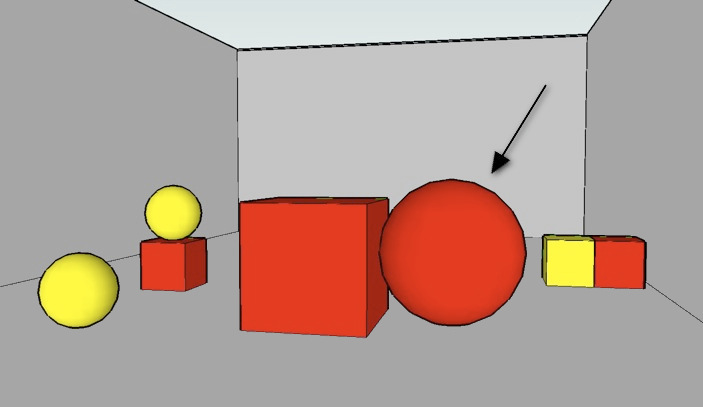
\includegraphics[width=\textwidth]{images/22sinletrasClaro.jpg}
  \caption{}\label{GRE3D7-stimulus1}
\end{subfigure}%
\begin{subfigure}{.5\textwidth}
 \centering
\begin{tabular}{l}
 {\it La esfera grande}\\

 {\it La esfera roja que est\'a al lado del cubo rojo} \\

 {\it El objeto que est\'a al lado del cubo grande}\\

 {\it La bola roja}\\

 {\it La pelota a la izquierda del cubo amarillo}\\

 {\it La bola grande}\\

 {\it La esfera que est\'a a la derecha del cubo rojo y a }\\
{\it la izquierda del cubo amarillo}\\

 {\it La cosa que est\'a a la derecha del cubo del medio}\\

  {\it ...}
 \end{tabular}
\hspace*{-30cm}
\centering\caption{}\label{er-figura1}
\end{subfigure}
\begin{centering}
\caption{Expresiones referenciales que identifican al objeto se\~nalado por la flecha.}
\label{figura-er}
\end{centering}
\end{figure}

La \textbf {generaci\'on de expresiones referenciales (GER)} entre todas las subtareas de GLN, es una de las que ha recibido m\'as atenci\'on. En la pr\'actica, la mayor\'ia de los sistemas de GLN, con independencia de su finalidad, contiene un m\'odulo de GER de alg\'un tipo~\cite{Mellish2004}. Esto no es sorprendente
en vista del papel central que las expresiones referenciales tienen en la comunicaci\'on. Un sistema que proporciona
consejos sobre los viajes a\'ereos \cite{white2010generating} tiene que hacer referencia a los vuelos ---{\it el vuelo m\'as barato}, {\it un vuelo directo}---, un sistema de navegaci\'on para autom\'oviles~\cite{Drager:2012:GLN:2380816.2380908}
necesita generar descripciones espaciales ---{\it tomar el puente junto a la iglesia, a la derecha}---,
y un robot que ensambla piezas de juguetes junto con un usuario humano~\cite{foster-etal-ijcai2009} debe hacer referencia a los componentes ---{\it inserte el perno verde hasta el final en el cubo rojo}. Cuando hablamos, nos referimos a cosas (tangibles como un puente, o intangibles como una fecha), es decir generamos expresiones referenciales. Un sistema que genera texto, tambi\'en deber\'a generar expresiones referenciales. La generaci\'on autom\'atica de expresiones referenciales es el tema de esta tesis.

Un sistema de GLN incluye 3 etapas: {\bf determinaci\'on de contenido} ---qu\'e decir--- {\bf lexicalizaci\'on} ---con qu\'e palabras--- y {\bf realizaci\'on ling\"{u}\'istica} ---c\'omo decirlo. La determinaci\'on de contenido, elige qu\'e informaci\'on incluir en la oraci\'on. La lexicalizaci\'on elige qu\'e lexemas usar para comunicar el contenido determinado por la etapa anterior. Y la realizaci\'on arma la oraci\'on agregando los art\'iculos, preposiciones, y dem\'as palabras funcionales necesarias y orden\'andolas de forma tal que la frase resultante sea gramaticalmente aceptable. 

Un sistema de GER, tiene esas 3 etapas tambi\'en: {\bf determinaci\'on de contenido} ---decide qu\'e propiedades o relaciones del objeto a describir se incluir\'an en la expresi\'on referencial--- {\bf lexicalizaci\'on} ---elige las palabras que se van a usar para nombrar las propiedades y relaciones--- y {\bf realizaci\'on ling\"u\'istica} ---se encarga de armar el sintagma nominal para que sea gramaticalmente correcto.

Por ejemplo, la primer ER de la Figura \ref{figura-er} incluye las propiedades {\it tama\~no} y {\it forma} del objeto se\~nalado por la flecha, lexicalizadas como {\it grande} y {\it esfera} respectivamente y realizadas agregando el art\'iculo {\it la} antes de {\it esfera}, e incluyendo el sustantivo {\it esfera} antes que el adjetivo {\it grande}; formando as\'i el sintagma nominal {\it La esfera grande} que es correcto en espa\~nol. Otra lexicalizaci\'on y realizaci\'on de las mismas propiedades ---es decir, de la misma sem\'antica--- podr\'ia ser {\it La bola de gran tama\~no}. A lo largo de esta tesis usaremos el t\'ermino {\bf expresi\'on referencial} (ER) para nombrar la salida de cualquiera de las 3 etapas de la GER. Es decir, llamaremos expresi\'on referencial al conjunto de propiedades y relaciones que refieren un\'ivocamente a un objeto aunque no est\'en lexicalizadas o realizadas.

En lo que sigue introduciremos terminolog\'ia b\'asica, relacionada con la GER que nos servir\'a a lo largo de toda la tesis para entendernos.

El {\bf dominio} de una ER define los tipos de entidades que est\'an siendo contemplados. Por ejemplo el dominio de la Figura \ref{figura-er} son las figuras geom\'etricas en 3 dimensiones. En particular, el dominio incluye cubos y esferas de colores rojo y amarillo, algunas grandes y otras peque\~nas, situadas en un entorno con perspectiva.

El {\bf contexto} de una ER contiene un subconjunto de las entidades del dominio. La Figura \ref{figura-er} muestra un contexto con 7 entidades del dominio, 4 rojas y 3 amarillas. Otros ejemplos son los puntos de referencia visibles en un cierto momento en un camino para el que estamos dando direcciones, un subconjunto de las fotograf\'ias utilizadas en una configuraci\'on experimental, o los ingredientes de cocina que ya se han mencionado en una receta. En un dominio visual, el contexto, incluyendo las propiedades de sus objetos y su configuraci\'on espacial, se puede llamar \textbf{escena}. %El contexto de la Figura \ref{GRE3D7-stimulus1} son los todos los objetos visibles con sus propiedades.

Cada {\bf entidad} del contexto (tambi\'en conocido como objeto o elemento) tiene un tipo ---\emph{esfera}--- ciertas propiedades o caracter\'isticas ---\emph{color}---, valores de esas propiedades ---\emph{rojo}---, y puede tener relaciones con otros objetos ---\emph{a la derecha de}. Una {\bf propiedad} (unaria) es una caracter\'istica de una entidad particular. Por ejemplo, la raza de un perro, el tener o no tener bigotes para un hombre, o el color para un objeto. Cada entidad puede tener muchas propiedades, y puede tener relaciones (tambi\'en llamadas: propiedades binarias), por ejemplo con respecto a la posici\'on f\'isica, como estar situado al lado de otro objeto. 

El {\bf target} (u objetivo), es el subconjunto de objetos de un contexto a los cuales queremos referirnos. En la escena del ejemplo de la Figura \ref{figura-er}, el target es el objeto se\~nalado por la flecha. En este caso, el target es un conjunto singleton, es decir tiene un s\'olo elemento. Si el target tiene m\'as de un elemento, las ERs que lo identifican son plurales.

Dado un contexto, un target y una descripci\'on (parcial) del target, los {\bf distractores} son otros elementos que se encuentran en el contexto, y que tambi\'en cumplen con la descripci\'on parcial. Si la descripci\'on parcial es {\it esfera} las esferas que no son el target de la Figura \ref{figura-er} son  distractores, y por ello es necesario seguir agregando propiedades o relaciones para identificar un\'ivocamente al target.

Un {\bf algoritmo} para GER, es un procedimiento autom\'atico que toma, al menos, alg\'un tipo de representaci\'on de un contexto y un target, y da como resultado una (o m\'as) expresi\'on(es) referencial(es) para el target considerado, si puede identificarlo un\'ivocamente en el contexto.

Una computadora que se enfrenta a la tarea de generar autom\'aticamente expresiones referenciales en un contexto determinado, necesitar\'a una representaci\'on de todos los objetos de la Figura \ref{figura-er} y las propiedades de cada uno de ellos. En la Figura~\ref{contexto-tabla-propiedades} se muestra una posible forma de representar los objetos, sus propiedades y relaciones: una base de datos que contiene todas las propiedades relevantes de los objetos de la escena. Entonces, la tarea de GER para el objeto $e_5$ involucra encontrar alguna combinaci\'on de valores de propiedades y relaciones con otros objetos, que aplique \'unicamente a $e_5$, y no a los otros objetos. Como dijimos, esta tarea de encontrar las propiedades y relaciones que aplican a un target y no a los distractores, se llama {\emph selecci\'on de contenido para la generaci\'on de una expresi\'on referencial}. Mirando la Tabla \ref{tabla-propiedades} podemos decir que {\it red ball}, {\it large ball} y {\it large red ball} son algunas ERs del objeto $e_5$, cuyas realizaciones en espa\~{n}ol podr\'ian ser: {\it La bola roja}, {\it La esfera grande} y {\it La esfera grande y roja}. {\it La bola roja} y {\it La esfera grande} aparecen entre las ERs dadas por las personas listadas en la Figura \ref{figura-er}.
%Como una primera intuici\'on podemos ver que la Figura \ref{formula-subgrafo} es un subrafo de la Figura \ref{representacion-modelo} que identifica un\'ivocamente al target, representa la cuarta ER mostrada en la Figura \ref{er-figura1}. Y la Figura \ref{formula-subgrafo2} tambi\'en identifica al target un\'ivocamente y representa la segunda ER mostrada en \ref{er-figura1}.
%que est\'an dadas en la Figura \ref{er-figura1} son muchas m\'as de las que mostramos en las f\'ormulas de la Figura \ref{er-figura1-b}, esto nos lleva a pensar que un algoritmo puede que no consiga la variedad que las personas dan. La representaci\'on ilustrada en la Figura~\ref{representacion-modelo} es equivalente a la mostrada en la Tabla \ref{tabla-propiedades}.

%\vspace*{-1.5cm}
\begin{figure}[h]
\begin{subfigure}{.45\textwidth}
  \centering
	\vspace*{-.2cm}
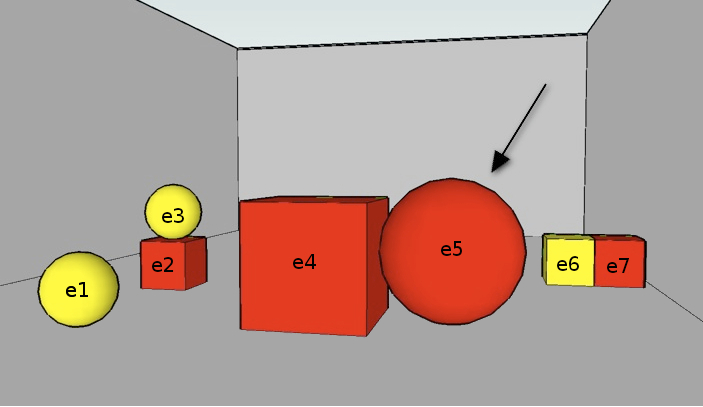
\includegraphics[width=\textwidth]{images/22.jpg}
  \caption{}\label{GRE3D7-stimulus1-ids}
\end{subfigure}
\begin{subfigure}{1\textwidth}
% \centering
%\begin{centering}
\hspace*{-16cm}
\begin{scriptsize}
\begin{tabular}{|l|c|c|c|c|c|c|c|}
\hline
\textbf {id}& 	\textbf {type}		&	\textbf {color}	&	\textbf {size}& \textbf {rigth} & \textbf {left} & \textbf {ontop}	& \textbf {below}	\\
   	   &  	    			&	    		&	     		&  \textbf {of}   		 &  \textbf {of}	    &  	&  \\
\hline \hline
$e_1$ & ball & yellow & small & - & - & - & - \\
$e_2$ & cube & red & small & - & - &- & $e_3$ \\
$e_3$ & ball & yellow & small & - & - & $e_2$ & -\\
$e_4$ & cube & red & large & - & $e_5$ & - & -\\
$e_5$ & ball & red & large & $e_4$ & - & - & -\\
$e_6$ & cube & yellow & small & - & $e_7$ & - & -\\
$e_7$ & cube & red & small & $e_6$ & - & - & -\\
\hline
%&&&&&&&\\
%&&&&&&&\\

\end{tabular}
\end{scriptsize}
\vspace*{1cm}
%\center
\centering \hspace*{-8cm} \caption{}\label{tabla-propiedades}
%\end{centering}
\end{subfigure}
\caption{Formalizaci\'on de las propiedades de la escena en una tabla de doble entrada.}\label{contexto-tabla-propiedades}
\end{figure}

En la pr\'oxima secci\'on veremos porqu\'e la tarea de GER es m\'as compleja de lo que parece a primera vista y en la siguiente introduciremos c\'omo herramientas de teor\'ia de modelos nos pueden ayudar.

\section{Expresiones referenciales bajo incertidumbre}
\label{sec:gre-incertidumbre}


%Los conjuntos son dif\'icil para referirse a, por ejemplo, y algoritmos
%diseñado para tratar con ellos lograr una menor semejanza humana cuando se refiere a los conjuntos de
%a los objetos individuales (van Deemter et al., en prensa). Los recientes esfuerzos para dejar que los algoritmos REG
%referirse a las regiones espaciales sugieren que en dominios grandes, realista, identificación precisa de
%un objetivo es un objetivo que se puede aproximar, pero rara vez alcanzado (Turner et al., 2008;
%Turner, Sripada, y Reiter 2009) .Es en tales dominios que prominencia (especialmente en el
%sentido no lingüístico) se convierte en un problema crítico. 
Cuando la generaci\'on de expresiones referenciales ocurre en la vida real, en lugar de ocurrir en un experimento controlado, las fuentes de \textbf{incertidumbre} que afectan al proceso se multiplican. En trabajo 
reciente en el \'area de GER \cite{turner2008,turner2009} se discute que, al intentar usar algoritmos de GER en dominios grandes 
y realistas (como por ejemplo la descripci\'on de regiones en mapas) la identificaci\'on precisa del target es una tarea que puede ser 
aproximada pero raramente lograda. Los autores argumentan que esto se debe, en parte, a que las representaciones geogr\'aficas 
son necesariamente \textbf{incompletas}. Esta falta de informaci\'on introduce incertidumbre (por ejemplo, el restaurante se\~nalado por la flecha en la Figura \ref{target_mapa}, ?`es realmente el \'unico restaurante de esa calle? o ?`es el \'unico que aparece en el mapa?).

\begin{figure}[h]
\centering
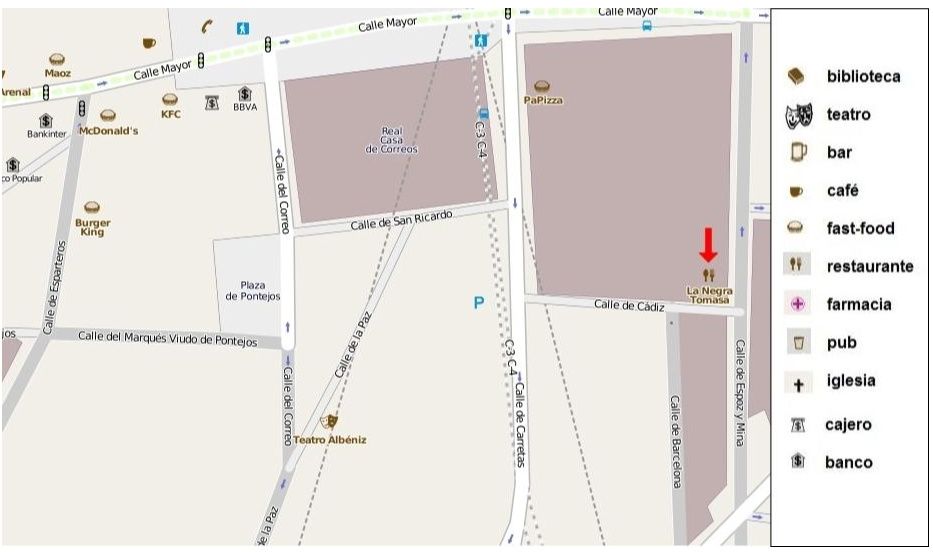
\includegraphics[width=\textwidth]{images/corpus/mapa15.png}
\caption{Ejemplo de target en el contexto de un mapa del ZOOM corpus.}
\label{target_mapa}
\end{figure}

Cuando la informaci\'on del contexto proviene de datos de sensores, las entradas del algoritmo de GER son inevitablemente ruidosas. Es decir, 
contienen informaci\'on no s\'olo incompleta sino tambi\'en posiblemente {\bf incorrecta}. Incluso en contextos tan simples como el de la 
Figura \ref{figura-er} hay incertidumbre. ?`La Figura \ref{representacion-modelo1} representa toda la informaci\'on del 
contexto?. Algunos podemos opinar que s\'i, otros que no. 

\begin{figure}[h]
%\begin{subfigure}{.5\textwidth}
  \centering
\vspace*{1cm}
\begin{picture}(250,50)
\put(0,-50){\begin{tikzpicture}
  [
    n/.style={circle,draw,inner sep=1.5pt,node distance=1.5cm},
		 aArrow/.style={->, >=stealth, semithick, shorten <= 1pt, shorten >= 1pt},
  ]
 \node[n,label=below:{
    \relsize{-2}$\begin{array}{c}
      \nSmall\\[-3pt] 
      \nYellow \\[-3pt] 
      \nBall\end{array}$}] (a) {$e_1$};
 \node[n,label=below:{
    \relsize{-2}$\begin{array}{c}     
      \nSmall\\[-3pt] 
      \nRed\\[-3pt] 
      \nCube\end{array}$}, right of=a] (b) {$e_2$};
 \node[n,label=above:{
    \relsize{-2}$\begin{array}{c}     
      \nSmall\\[-3pt] 
      \nYellow\\[-3pt] 
      \nBall\end{array}$}, above of=b] (c) {$e_3$};
 \node[n,label=below:{
    \relsize{-2}$\begin{array}{c}
      \nLarge\\[-3pt] 
      \nRed\\[-3pt] 
      \nCube\end{array}$}, right of=b] (d) {$e_4$};
 \node[n,label=below:{
    \relsize{-2}$\begin{array}{c}
      \nLarge\\[-3pt] 
      \nRed\\[-3pt] 
      \nBall\end{array}$}, right of=d] (e) {$e_5$};
 \node[n,label=below:{
    \relsize{-2}$\begin{array}{c}
      \nSmall\\[-3pt] 
      \nYellow\\[-3pt] 
      \nCube\end{array}$}, right of=e] (f) {$e_6$};
 \node[n,label=below:{
    \relsize{-2}$\begin{array}{c}
      \nSmall\\[-3pt]
      \nRed\\[-3pt] 
      \nCube\end{array}$},  right of=f] (g) {$e_7$};
 \draw [aArrow,bend right=40] (b) to node[auto,swap]{\relsize{-3}$\nBelow$} (c);
 \draw [aArrow,bend right=40] (c) to node[auto,swap]{\relsize{-3}$\nOntop$} (b);
 \draw [aArrow,bend right=40] (d) to node[auto,swap]{\relsize{-3}$\nLeftof$} (e);
 \draw [aArrow,bend right=40] (e) to node[auto,swap]{\relsize{-3}$\nRightof$} (d);
 \draw [aArrow,bend right=40] (f) to node[auto,swap]{\relsize{-3}$\nLeftof$} (g);
 \draw [aArrow,bend right=40] (g) to node[auto,swap]{\relsize{-3}$\nRightof$} (f);
 %\draw[dotted] (-0.5,-1.3) rectangle (8,3.1);
 \draw[dotted] (-0.5,-1.5) rectangle (8,3);
 \end{tikzpicture}}
 \end{picture}
 %\end{flushleft}

\vspace*{1.5cm} 
\caption{Formalizaci\'on de las propiedades de la Figura \ref{figura-er} como un grafo etiquetado.}\label{representacion-modelo1}
\end{figure}


En efecto, la persona que gener\'o la ER {\it La pelota a la izquierda del cubo amarillo} opina que no: la relaci\'on \emph{a la izquierda de} entre el target y el cubo amarillo no est\'a representada en el grafo. Un algoritmo de GER con este grafo como input no puede generar esta expresi\'on referencial. La informaci\'on disponible no s\'olo impide la generaci\'on de ERs v\'alidas, sino que tambi\'en permite la generaci\'on de ERs claramente incorrectas como \emph{La esfera roja 
que no tiene nada a la derecha}.
El grafo puede completarse para que sea posible
generar la expresi\'on referencial. El grafo resultante se ilustra en la Figura \ref{representacion-modelo-completo}. Sin embargo, este grafo tampoco es completo, 
de hecho, la ER {\it la cosa que est\'a a la derecha del cubo del medio} no se podr\'ia generar con este grafo. 

\begin{figure}[h]
%\begin{subfigure}{.5\textwidth}
\centering
%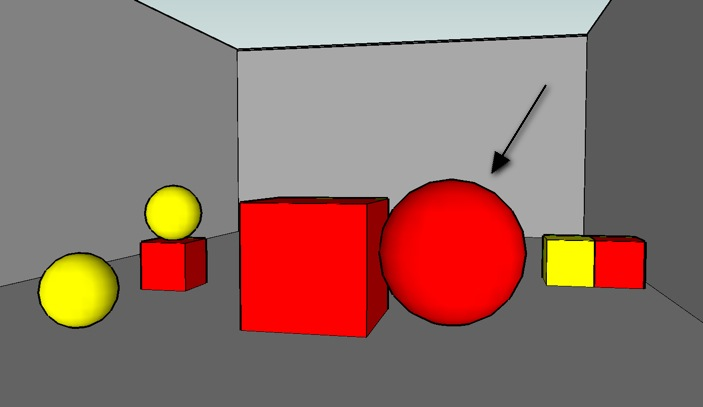
\includegraphics[width=\textwidth]{images/22sinletras.jpg}
%%\caption{Ejemplo de contexto}
%\label{GRE3D7-stimulus1-b}
\vspace*{1cm}
\begin{picture}(250,50)
\put(0,-50){\begin{tikzpicture}
  [
    n/.style={circle,draw,inner sep=1.5pt,node distance=1.5cm},
		 aArrow/.style={->, >=stealth, semithick, shorten <= 1pt, shorten >= 1pt},
  ]
 \node[n,label=below:{
    \relsize{-2}$\begin{array}{c}
      \nSmall\\[-3pt] 
      \nYellow \\[-3pt] 
      \nBall\end{array}$}] (a) {$e_1$};
 \node[n,label=below:{
    \relsize{-2}$\begin{array}{c}     
      \nSmall\\[-3pt] 
      \nRed\\[-3pt] 
      \nCube\end{array}$}, right of=a] (b) {$e_2$};
 \node[n,label=above:{
    \relsize{-2}$\begin{array}{c}     
      \nSmall\\[-3pt] 
      \nYellow\\[-3pt] 
      \nBall\end{array}$}, above of=b] (c) {$e_3$};
 \node[n,label=below:{
    \relsize{-2}$\begin{array}{c}
      \nLarge\\[-3pt] 
      \nRed\\[-3pt] 
      \nCube\end{array}$}, right of=b] (d) {$e_4$};
 \node[n,label=below:{
    \relsize{-2}$\begin{array}{c}
      \nLarge\\[-3pt] 
      \nRed\\[-3pt] 
      \nBall\end{array}$}, right of=d] (e) {$e_5$};
 \node[n,label=below:{
    \relsize{-2}$\begin{array}{c}
      \nSmall\\[-3pt] 
      \nYellow\\[-3pt] 
      \nCube\end{array}$}, right of=e] (f) {$e_6$};
 \node[n,label=below:{
    \relsize{-2}$\begin{array}{c}
      \nSmall\\[-3pt]
      \nRed\\[-3pt] 
      \nCube\end{array}$},  right of=f] (g) {$e_7$};
 \draw [aArrow,bend right=40] (b) to node[auto,swap]{\relsize{-3}$\nBelow$} (c);
 \draw [aArrow,bend right=40] (c) to node[auto,swap]{\relsize{-3}$\nOntop$} (b);
 \draw [aArrow,bend right=40] (d) to node[auto,swap]{\relsize{-3}$\nLeftof$} (e);
 \draw [aArrow,bend right=40] (e) to node[auto,swap]{\relsize{-3}$\nRightof$} (d);
 \draw [aArrow,bend right=40] (f) to node[auto,swap]{\relsize{-3}$\nLeftof$} (g);
 \draw [aArrow,bend right=40] (g) to node[auto,swap]{\relsize{-3}$\nRightof$} (f);
 
 \draw [aArrow,bend right=40] (a) to node[auto,swap]{} (b);
 \draw [aArrow,bend right=40] (b) to node[auto,swap]{} (a);

 \draw [aArrow,bend right=40] (b) to node[auto,swap]{} (d);
 \draw [aArrow,bend right=40] (d) to node[auto,swap]{} (b);

\draw [aArrow,bend right=40] (e) to node[auto,swap]{} (f);
 \draw [aArrow,bend right=40] (f) to node[auto,swap]{} (e);
 %\draw[dotted] (-0.5,-1.3) rectangle (8,3.1);
 \draw[dotted] (-0.5,-1.5) rectangle (8,3);
 \end{tikzpicture}}
 \end{picture}
 %\end{flushleft}

\vspace*{2cm} 
 \caption{Representaci\'on de contexto m\'as completo.}\label{representacion-modelo-completo}
\end{figure}


Aunque no hablemos ni de incompletitud ni de incorrectitud tambi\'en hay incertidumbre en \textbf{cu\'al} de todas las posibles ERs un sistema de GER debe 
elegir. Por ejemplo seguramente hay personas que preferir\'an ERs que usen la palabra \emph{esfera}, antes que \emph{bola}. Y seguramente 
no falte quien diga que \emph{la} mejor expresi\'on referencial ni si quiera aparece en la Figura \ref{figura-er}. Sin embargo, seguramente 
habr\'a una tendencia como se muestra en estudios previos \cite{viet:gene11}. Nadie preferir\'a una ER que use 21 propiedades y 6 relaciones 
para describir al target de la Figura \ref{figura-er}.

El largo de una ER afecta su calidad. Se podr\'{i}a pensar, por ejemplo, que las referencias son \'optimas cuando son \textbf{m\'{i}nimas}
 en longitud, es decir, cuando contienen s\'olo informaci\'on suficiente para identificar el objeto target y nada m\'as. Pero la generaci\'on de referencias m\'{i}nimas
no es lo que las personas hacen ni lo que es m\'as \'util para los oyentes, como se muestra en trabajo previo \cite{Lu_sasha2015}. Y ni si quiera 
nos resuelve el problema de elegir una ER. {\it La bola grande} y {\it La esfera roja} son dos ERs de la Figura \ref{figura-er} y tienen 
exactamente la misma longitud.

Dado que la incertidumbre es inherente a la tarea de GER, lo mejor que se puede hacer es que un algoritmo de GER devuelva un \textbf{ranking}
 de ERs, o lo que es lo mismo, un conjunto de ERs en el que cada ER tiene un valor asociado que intenta reflejar cu\'an buena es esa ER para el input dado.

?`Como podemos generar un ranking de ERs?.
Un algoritmo simplista generar\'ia primero todas las ERs posibles y luego las ordenar\'ia con alg\'un criterio. Esto es posible porque la cantidad de ERs es finita dado un modelo finito, pero esta cantidad puede ser muy grande, exponencial en el tama\~{n}o del modelo y la gran mayor\'ia de estas ERs no se llegar\'ian a usar en una aplicaci\'on real. Una aplicaci\'on s\'olo usar\'a las mejores ERs de un target considerado.
Una forma m\'as eficiente de generar un ranking de ERs es dise\~{n}ar un algoritmo no determin\'istico y correrlo una cantidad de veces suficiente para la aplicaci\'on.

Un algoritmo para la GER es {\bf no-determin\'istico} si puede dar diferentes ERs para el mismo contexto y target en sucesivas ejecuciones. 
Para producir un ranking de las mejores ERs para un target, el no determinismo debe estar guiado de alguna forma que le permita dar m\'as veces ERs m\'as frecuentes, y menos veces las menos frecuentes. Llamaremos a esta gu\'ia: \textbf{probabilidad de uso} de una propiedad o relaci\'on. Esta probabilidad se puede ver afectada por caracter\'isticas de la propiedad o relaci\'on (tipos de propiedades) o por caracter\'isticas de qui\'en interpretar\'a la ER (el interlocutor).

Hay diferentes \textbf{tipos de propiedades}, por ejemplo taxon\'omicas (las que tiene el objeto, como \emph{esfera}, o \emph{roja}), relacionales (las que necesitan dar una expresi\'on de otro objeto, por ejemplo {\it estar al lado de}), vagas (son las m\'as dif\'iciles de identificar, por ejemplo: \emph{chico}, \emph{grande}, no son propiedades absolutas, ya que necesitan un contexto, ?`con respecto a qu\'e algo es chico o grande?). Ciertos valores de propiedades pueden ser m\'as f\'aciles de identificar que otros, por ejemplo cierto color verde podr\'{i}a ser m\'as complicado de identificar que el tama\~no grande de un objeto. Notar que cuando decimos el tama\~no, tenemos como marco de referencia a los objetos de la escena, en ese contexto un objeto es {\it grande}.
%En esta tesis estudiamos la generaci\'on autom\'atica de expresiones referenciales, 
%primero mostramos c\'omo podemos a\~nadir no determinismo a los algoritmos estudiados. Los algoritmos de refinamiento estudiados, tienen un orden fijo en el cual consideran las propiedades y relaciones, y la naturalidad de las expresiones referenciales que generan depende de este orden particular considerado, nosotros proponemos reemplazar ese orden fijo sobre las propiedades y/o relaciones de la escena de entrada por una~\emph{probabilidad de uso} para cada propiedad y/o relaci\'on, y modificar los algoritmos para que tengan en cuenta esas propiedades. De esta manera, cada llamada al algoritmo puede producir diferentes ERs para la misma escena y target de entrada. 

%Es decir nuestra meta, no s\'olo ser\'a crear algoritmos para la generaci\'on autom\'atica de expresiones referenciales, sino crearlos de tal manera que podamos imitar en gran medida lo que dir\'ian las personas.
%
%Mostraremos que dado un corpus (como el corpus GRE3D7 o el TUNA de los cuales hablaremos en Cap\'itulo~\ref{sec:seleccion}) podemos estimar estas probabilidades de uso de manera que las ER se generen con una distribuci\'on de probabilidad que coincide en gran medida con las que se encuentra en el corpus.

Esta selecci\'on de la ER m\'as apropiada tambi\'en debe tener en cuenta al \textbf {interlocutor}, es natural que los humanos demos distintas ERs a distintos interlocutores.
% En el \'area muchas veces se habla de optimalidad de la ER, pero con diferentes significados, para algunos una ER \'optima es aquella que dice lo m\'inimo necesario para identificar al objeto target, para otros es la menos esfuerzo requiere del interlocutor para identificarlo.
La selecci\'on de qu\'e propiedades y/o relaciones con otros objetos incluir en una expresi\'on referencial depender\'a del prop\'osito que tengamos para dicha expresi\'on referencial. Una expresi\'on referencial ser\'a muy distinta si nuestro objetivo es dar la m\'inima informaci\'on que distinga al objeto, que si nuestro objetivo es ayudar al interlocutor a que identifique el objeto.

La generaci\'on de expresiones referenciales en el mundo real sufre de diversas fuentes de incertidumbre. En esta tesis proponemos formas para modelar esta incertidumbre partiendo de t\'ecnicas de representaci\'on de conocimiento basadas en teor\'ia de modelos.
%En la vida real hay muchas cosas que nos ayudan a darnos cuenta si nuestro interlocutor identific\'o el objeto target, como ser la expresi\'on de duda nos dar\'ia una pauta de que no esta entendiendo lo que le queremos decir...
%
%\textbf{FALTA CIERRE A ESTA SECCION!}

%En esta tesis nos vamos a enfocar en la selecci\'on de contenidos de las expresiones referenciales, y el objetivo ser\'ia simular el comportamiento humano, para ello vamos a usar corpus de expresiones referenciales para aprender como realizan esta tarea las personas.
 %
%Las propiedades y relaciones de los objetos de la escena forman una base de conocimento, estos datos se pueden organizar en jerarqu\'ias, por ejemplo: conjunto de animales, conjunto de mamiferos, conjunto de insectos. Algunos conjuntos pueden estar contenidos en otros, es decir algunos objetos o entidades pueden compartir caracter\'isticas.
%
%Si el objeto target tiene la propiedad de medir 1.80 de alto, y est\'a en un grupo donde los dem\'as son m\'as peque\~nos, es m\'as natural decir el m\'as alto, que el que mide 1.80.
%Si tenemos 100 caracter\'isticas de una persona, y con esas caracter\'isticas se pudiera identificar un\'ivocamente a una persona, un sistema que diera que las 100 caracter\'isticas no ser\'ia un sistema que suene muy natural, ya que una persona no dar\'ia 100 propiedades para identificar a una persona particular. As\'i podr\'iamos decir que las expresiones referenciales variaran seg\'un la cantidad de informaci\'on que contienen, si contienen la m\'inima informaci\'on para identificarlas un\'ivocamente ser\'an minimales, si contienen m\'as informaci\'on estar\'an sobreespecificadas, pero en el caso de contener m\'as de la m\'inima informaci\'on para identificarlas un\'ivocamente... cu\'anta m\'as dar?, intentaremos imitar lo que hacen las personas cuando dan expresiones referenciales para responder este tipo de preguntas.
%El sistema deber\'ia tener una lista del orden de preferencia de los atributos a usar.\\ 



%NO NO Las primeras investigaciones en GER no voy a poner esto porque no quiero pasar por alto shrdlu de vinogran 1969
%\cite{C92-1038}; \cite{Dale95computationalinterpretations} hicieron una serie de supuestos simplificadores, por ejemplo no usaban relaciones, el target era un s\'olo objeto, y como resultado los primeros
%algoritmos GER s\'olo pod\'ian generar una variedad limitada de expresiones referenciales. Cuando
%los investigadores comenzaron a levantar algunos de estos supuestos, esto di\'o lugar a algoritmos de GER
%con un repertorio m\'as amplio, siendo capaces de generar, por ejemplo, plurales y expresiones relacionales. 
%
%Este movimiento ha creado una serie de nuevos desaf\'ios, sin embargo. Por ejemplo, el
%n\'umero de formas en las que uno puede referirse a un conjunto de objetos de destino aumenta, por lo que la elecci\'on de una
%buena expresi\'on referencial es m\'as dif\'icil.
%
%Del mismo modo, incluso propuestas recientes tienden a asumir que no es problem\'atico para determinar qu\'e informaci\'on
%es compartida entre el hablante y el oyente.\\
%(a) C\'omo se representa la informaci\'on del dominio?\\
%(b) C\'omo se representa el contenido sem\'antico de una expresi\'on referencial? \\
%(c) C\'omo se pueden encontrar descripciones distintivas?
%
%En los contextos de los corpus analizados en esta tesis, nos encontramos con cuatro tipos diferentes de atributos:
%tipos de objetos, atributos absolutos, atributos relativos, atributos espaciales incluidas las relaciones y atributos de localizaci\'on.
%
%El tipo de un objeto constituye un caso especial, ya que es muy rara vez omite
%en la expresi\'on referencial. En consecuencia, la mayor\'ia de los algoritmos tratan de
%considerarlo por separado para asegurarse de que se a\~nade a cada expresi\'on referencial. Una explicaci\'on parcial para esta condici\'on especial es que las expresiones referenciales se realizan como sintagmas nominales,
%cada sintagma nominal requiere un sustantivo, y por lo general es el tipo del referente dado que es el sustantivo principal.
%
%\section{Contribuciones de esta tesis}
%\label{sec:contribiciones}
%\textcolor{blue}{Esta parte se va?}
%\begin{itemize}
%\item Se estudi\'o el avance en el \'area de la generaci\'on autom\'atica de expresiones referenciales, los algoritmos existentes y los problemas que ellos ten\'ian, las aproximaciones emp\'iricas realizadas en el \'area en el Cap\'itulo~\ref{sec:seleccion}.
%\item Se estudiaron las m\'etricas de evaluaci\'on tanto autom\'aticas como manuales en el Cap\'itulo~\ref{sec:seleccion}, las cuales ser\'an luego aplicadas en el Cap\'itulo~\ref{sec:evaluacion}.
%%\item Se abordaron los siguientes problemas: no-determinismo, sobreespecificaci\'on.
%\item Se estudiaron estudiaron distintas l\'ogicas y sus lenguajes asociados, se compararon esos lenguajes con el lenguaje utilizado para dar ER, a fin de elegir una l\'ogica apropiada en el Cap\'itulo~\ref{sec:intro_logica}.
%\item Se seleccion\'o un algoritmo existente al cual se le agregaron probabilidades de uso para simular el no-determinismo encontrado en corpus. Este fue seleccionado por permitirmos agregar los aspectos tenidos en cuenta en esta tesis: dar un algoritmo que aborde el no-determinismo, la sobreespecificaci\'on que sea relacional, que genere plurales en el Cap\'itulo~\ref{sec:learning}.
%%\item Se modific\'o el algoritmo para que sea no-determinista.
%\item Se agreg\'o sobreespecificaci\'on al algoritmo permitiendo agregar propiedades o relaciones cuando estas tienen una alta probabilidad de uso en corpus. Y al mismo tiempo se agura la terminaci\'on en el Cap\'itulo~\ref{sec:algoritmo}.
%\item Se propone un m\'etodo para calcular las probabilidades de uso (\puse)\ de las relaciones del modelo el cual genera una distribuci\'on de expresiones referenciales cercana a la encontrada en el corpus.
%\item Se prob\'o el algoritmo en 2 corpus existentes (el GRE3D7 y el Tuna corpus) en el Cap\'itulo~\ref{sec:evaluacion}.
%\item Se realiz\'o una evaluaci\'on en la que se compararon las salidas del algoritmo con ambos corpus. Se usaron m\'etricas autom\'aticas y manuales Cap\'itulo~\ref{sec:evaluacion}.
%\item Se creo un corpus de descripciones de mapas (el ZOOM corpus).
%\item Se hizo un caso de estudio de 3 mapas del ZOOM corpus explicado en Cap\'itulo~\ref{sec:corpus}, en el cual se toma 1 mapa con target singular, el mismo mapa con zoom 2x y target singular y el mismo mapa con target plural.
%\end{itemize}



\section{Expresiones referenciales usando teor\'ia de modelos}
\label{sec:gre-teoria-modelos}

Los \textbf{modelos relacionales} tambi\'en conocidos como \textbf{modelos de kripke} y \textbf{modelos de primer orden} son muy utilizados para la representaci\'on de situaciones o escenas. 
Los modelos relacionales son grafos etiquetados y pueden verse tambi\'en como aut\'omatas finitos. Estas estructuras matem\'aticas han sido muy estudiadas y tienen muchas propiedades bien conocidas \cite{arec:hybr05b}. En esta tesis se adaptan algoritmos cl\'asicos de minimizaci\'on de aut\'omatas aplicados a la caracterizaci\'on de modelos relacionales.

Para un \textbf{vocabulario} de s\'imbolos relacionales r, un modelo relacional $\+M$ es una tupla $\tup{\Delta,\interp{\cdot}}$ donde:
\begin{itemize}
 \item $\Delta$ es un conjunto no vac\'io de objetos ---el dominio---
 \item $\interp{\cdot}$ es una funci\'on de interpretaci\'on, esto es, $\interp{r} \subseteq \Delta^n$ para todo s\'imbolo de relaci\'on $n$-ario $r$ que est\'a en el vocabulario.  
\end{itemize}
El \emph{tama\~no} de un modelo $\+M$ es la suma ($\#\Delta + \#\interp{\cdot}$), donde $\#\Delta$ es la cardinalidad
de $\Delta$ y $\#\interp{\cdot}$ es la suma de todas las aridades de las relaciones en $\interp{\cdot}$.
Si asumimos un vocabulario finito de s\'imbolos de relaci\'on $n$-arios entonces $\+M$ es \emph{finito}. 


%Un modelo relacional $\+M$ es una tupla 
%$\tup{\Delta,\interp{\cdot}}$ donde $\Delta$ es un conjunto no vac\'io, y
%$\interp{\cdot}$ es una funci\'on de interpretaci\'on, esto es,
%$\interp{r} \subseteq \Delta^n$ para todo s\'imbolo de relaci\'on $n$-aria tal que
%$r$ est\'a en el vocabulario. $\+M$ es \emph{finito} cuando
%$\Delta$ es finito.  El \emph{tama\~no} de un modelo $\+M$ es la suma
%$\#\Delta + \#\interp{\cdot}$, donde $\#\Delta$ es la cardinalidad
%de $\Delta$ y $\#\interp{\cdot}$ es la suma de todas las aridades de las
%relaciones en $\interp{\cdot}$.

A continuaci\'on vamos a presentar 2 ejemplos de modelos relacionales, uno en el que tenemos entidades \textbf{agentivas} (es decir, agentes animados que pueden realizar acciones) como perros y gatos, y otro en el que las entidades son \textbf{no agentivas}, es decir, son objetos est\'aticos.

El primer ejemplo se muestra en la Figura~\ref{fig:cat-dog-1} en la cual hemos representado un contexto
como un modelo relacional. Intuitivamente, $a$, $b$ y $d$ son perros, mientras que 
$c$ y $e$ son gatos;  $d$ es un peque\~no beagle; $b$ y $c$ tambi\'en son peque\~nos.
 Leeremos $\aSniffing(d,e)$ como ``{\em $d$ huele a $e$}''. La interpretaci\'on del s\'imbolo relacional $\nDog$ es $\interp{\nDog}$  =  $\cset{a,b,d}$ ya que $a$, $b$ y $d$ son los \'unicos perros del contexto. La interpretaci\'on de $\aSniffing$ es el conjunto de pares de elementos que cumplen $\aSniffing$. Por ejemplo ($a,a$) pertenece al conjunto dado que $a$ es un perro que se huele a s\'i mismo en el modelo.

 \begin{figure}[!ht]
 %\begin{center}
 \begin{tabular}{rcl}
$\Delta$               & = & $\cset{a,b,c,d,e}$\\
$\interp{\nDog}$      & = & $\cset{a,b,d}$\\
$\interp{\nCat}$      & = & $\cset{c,e}$\\
$\interp{\nBreed}$    & = & $\cset{d}$\\
$\interp{\aSmall}$    & = & $\cset{b,c,d}$\\
$\interp{\aSniffing}$ & = & $\cset{(a,a),(b,a),(c,b),(d,e),(e,d)}$
 \end{tabular}
\begin{picture}(90,30)
\put(0,-40){\begin{tikzpicture}
  [
    n/.style={circle,draw,inner sep=1.5pt,node distance=1.5cm},
    aSniffing/.style={->, >=stealth, semithick, shorten <= 3pt, shorten >= 3pt},
  ]
 \node[n,label=below:{\relsize{-1}$\begin{array}{c}\nDog\end{array}$}] (a) {$a$};

 \node[n,label=below:{\relsize{-1}$\begin{array}{c}\nDog\\ \aSmall \end{array}$}, right of=a] (b) {$b$};

 \node[n,label=below:{\relsize{-1}$\begin{array}{c}\nCat\\ \aSmall\end{array}$}, right of=b] (c) {$c$};

 \node[n,label=below:{\relsize{-1}$\begin{array}{c}\nDog\\ \nBreed\\  \aSmall \end{array}$}, right of=c] (d) {$d$};

 \node[n,label=below:{\relsize{-1}$\begin{array}{c}\nCat\end{array}$},right of=d] (e) {$e$};

 \draw [aSniffing,loop left] (a) to node[above,xshift=-5pt]{\relsize{-1}$\aSniffing$} (a);

 \draw [aSniffing,bend right=40] (b) to node[auto,swap]{\relsize{-1}$\aSniffing$} (a);

 \draw [aSniffing,bend right=40] (c) to node[auto,swap]{\relsize{-1}$\aSniffing$} (b);

 \draw[aSniffing, bend left=40] (d) to node[auto]{\relsize{-1}$\aSniffing$} (e);
 \draw[aSniffing, bend left=40] (e) to node[auto,swap]{\relsize{-1}$\aSniffing$} (d);

 \end{tikzpicture}}
 \end{picture}

 %\end{center}
 \caption{Representaci\'on de escena como un modelo relacional e interpretaci\'on de sus propiedades y relaciones. Ejemplo con entidades agentivas.\label{fig:cat-dog-1}}
 \end{figure}

El segundo ejemplo se muestra en la Figura~\ref{grafo-GRE3D7-stimulus_b} donde damos una posible representaci\'on de la escena de la Figura \ref{figura-er} como un modelo relacional. El dominio es $\Delta$  = $\cset{e_1,e_2,e_3,e_4,e_5,e_6,e_7}$. La interpretaci\'on de $\nBall$ es $e_1$, $e_3$ y $e_5$, ya que estos objetos son esferas, la de $\nCube$ es $\interp{\nCube}$ =$\cset{e_2, e_4, e_6, e_7}$, ya que esos objetos son cubos. Tenemos las relaciones $\nRightof$, $\nLeftof$, $\nBelow$ y $\nOntop$, cuyas interpretaciones se muestran en la figura. Como discutimos en la secci\'on anterior, se puede argumentar que este modelo est\'a incompleto, pero es suficiente para los objetivos ilustrativos de esta secci\'on.

\begin{figure}
\begin{flushleft}
\begin{tabular}{rcl}
$\Delta$              & = & $\cset{e_1,e_2,e_3,e_4,e_5,e_6,e_7}$\\
$\interp{\aRed}$      & = & $\cset{e_2,e_4,e_5,e_7}$\\
$\interp{\aYellow}$   & = & $\cset{e_1,e_3,e_6}$\\
$\interp{\nBall}$     & = & $\cset{e_1,e_3,e_6}$\\
$\interp{\nCube}$     & = & $\cset{e_2,e_4,e_6,e_7}$\\

$\interp{\aSmall}$    & = & $\cset{e_1,e_2,e_3,e_6,e_7}$\\
$\interp{\aLarge}$    & = & $\cset{e_4,e_5}$\\

$\interp{\nRightof}$   & = & $\cset{(e_4,e_5),(e_6,e_7)}$\\
$\interp{\nLeftof}$    & = & $\cset{(e_5,e_4),(e_7,e_6)}$\\
$\interp{\nOntop}$     & = & $\cset{(e_3,e_2)}$\\
$\interp{\nBelow}$     & = & $\cset{(e_2,e_3)}$\\

 \end{tabular}
\begin{picture}(120,50)
\put(0,-50){\begin{tikzpicture}
  [
    n/.style={circle,draw,inner sep=1.5pt,node distance=1.5cm},
		 aArrow/.style={->, >=stealth, semithick, shorten <= 1pt, shorten >= 1pt},
    %aSniffing/.style={->, >=stealth, semithick, shorten <= 3pt, shorten >= 3pt},
  ]
%\begin{tikzpicture}
%  [
%    n/.style={circle,fill,draw,inner sep=3pt,node distance=2cm},
%    aArrow/.style={->, >=stealth, semithick, shorten <= 1pt, shorten >= 1pt},
%  ]
 \node[n,label=below:{
    \relsize{-2}$\begin{array}{c}
      \nSmall\\[-3pt] 
      \nYellow \\[-3pt] 
      \nBall\end{array}$}] (a) {$e_1$};
 \node[n,label=below:{
    \relsize{-2}$\begin{array}{c}     
      \nSmall\\[-3pt] 
      \nRed\\[-3pt] 
      \nCube\end{array}$}, right of=a] (b) {$e_2$};
 \node[n,,label=above:{
    \relsize{-2}$\begin{array}{c}
      \nSmall\\[-3pt] 
      \nYellow\\[-3pt] 
      \nBall\end{array}$}, above of=b] (c) {$e_3$};
 \node[n,label=below:{
    \relsize{-2}$\begin{array}{c}
      \nLarge\\[-3pt] 
      \nRed\\[-3pt] 
      \nCube\end{array}$}, right of=b] (d) {$e_4$};
 \node[n,label=below:{
    \relsize{-2}$\begin{array}{c}
      \nLarge\\[-3pt] 
      \nRed\\[-3pt] 
      \nBall\end{array}$}, right of=d] (e) {$e_5$};
 \node[n,,label=below:{
    \relsize{-2}$\begin{array}{c}
      \nSmall\\[-3pt] 
      \nYellow\\[-3pt] 
      \nCube\end{array}$}, right of=e] (f) {$e_6$};
 \node[n,label=below:{
    \relsize{-2}$\begin{array}{c}
      \nSmall\\[-3pt]
      \nRed\\[-3pt] 
      \nCube\end{array}$},  right of=f] (g) {$e_7$};
 \draw [aArrow,bend right=40] (b) to node[auto,swap]{\relsize{-3}$\nBelow$} (c);
 \draw [aArrow,bend right=40] (c) to node[auto,swap]{\relsize{-3}$\nOntop$} (b);
 \draw [aArrow,bend right=40] (d) to node[auto,swap]{\relsize{-3}$\nLeftof$} (e);
 \draw [aArrow,bend right=40] (e) to node[auto,swap]{\relsize{-3}$\nRightof$} (d);
 \draw [aArrow,bend right=40] (f) to node[auto,swap]{\relsize{-3}$\nLeftof$} (g);
 \draw [aArrow,bend right=40] (g) to node[auto,swap]{\relsize{-3}$\nRightof$} (f);
 
%\draw[dotted] (-0.5,-1.3) rectangle (8,3.1);

% \end{tikzpicture}
%\caption{Grafo del contexto \ref{GRE3D7-stimulus}}
%\label{grafo-GRE3D7-stimulus_b}
%\end{figure}
 \end{tikzpicture}}
 \end{picture}
 \end{flushleft}
 \caption{Representaci\'on de la escena de la Figura \ref{figura-er} como un modelo relacional e interpretaci\'on de sus propiedades y relaciones. Ejemplo con entidades no agentivas.}
 \label{grafo-GRE3D7-stimulus_b}
 \end{figure}

Ahora nos enfocaremos en conseguir ERs para identificar a targets dados usando los modelos que acabamos de describir. Veremos lenguajes de distintas l\'ogicas y c\'omo las f\'ormulas l\'ogicas pueden representar a las ERs.
%Los lenguajes l\'ogicos son \'utiles para la tarea de describir (formalmente) elementos de una estructura relacional. 
A continuaci\'on definimos el lenguaje cl\'asico de la l\'ogica de primer orden (con desigualdad), \FOL. Dicho lenguaje se define inductivamente como sigue. Una f\'ormula $\phi$ es una f\'ormula de \FOL si es de alguna de las siguientes formas:

% *2 est\'a dado por $\top$ que es como decir 'cosa', todo elemento satisface $\top$, la desigualdad entre 2 elementos $ x_i$ y $x_j$, relaciones de tuplas, la negaci\'on de f\'ormulas de \FOL, la conjunci\'on de f\'ormulas de \FOL, y el existencial de una variable ligada en la f\'ormula de \FOL:
\begin{enumerate}
  \item $\top$ Es como decir {\it cosa}, todo elemento satisface $\top$.
  \item $x_i \not\approx x_j$ La desigualdad entre dos elementos $x_i$ y $x_j$.
  \item $r (\bar x)$ Relaciones de tuplas.
  \item $\lnot \gamma$ Negaci\'on de f\'ormulas.
  \item $\gamma \land \gamma'$ Conjunci\'on de f\'ormulas.
  \item $\exists x_i . \gamma$ Existencial de una variable ligada en la f\'ormula $\gamma$.
\end{enumerate}
%
donde $\gamma,\gamma' \in \FOL$,
$r$ es un s\'imbolo de relaci\'on $n$-aria y $\bar x$ es una tupla de $n$ variables.
Como es usual, $\gamma \lor \gamma'$ y $\forall x . \gamma$ son las versiones cortas de
$\lnot(\lnot\gamma \land \lnot\gamma')$ y $\lnot\exists x . \lnot\gamma$, respectivamente.
F\'ormulas de la forma $\top$, $x_i \not\approx x_j$ y $r(\bar
x)$ son llamados \emph{\'atomos}.%

Dado un modelo relacional $\+M = \tup{\Delta,\interp{\cdot}}$ y una
f\'ormula $\gamma$ con variables libres%
\footnote{%
    Asumimos que cada variable no puede aparecer libre y ligada a la vez, que una variable no est\'a ligada 2 veces,
    y que el \'indice de las variables crece en la f\'ormula de izquierda a derecha.%
}
$x_1\ldots x_n$, inductivamente definimos la \textbf{extensi\'on} o
\textbf{interpretaci\'on} de $\gamma$ como el conjunto de $n$-tuplas
 $\interp{\gamma}^n \subseteq \Delta^n$ que satisface:

\begin{enumerate}

\item $\interp{\top}^n$ $=$ $\Delta^n$

\item $\interp{x_i \not\approx x_j}^n$ $=$ $\cset{\bar{a} \mid \bar{a} \,{\in}\, \Delta^n, a_i \neq a_j}$

\item $\interp{\lnot\delta}^n$ $=$ $\Delta^n \setminus \interp{\delta}^n$

\item $\interp{r (x_{i_1} \ldots x_{i_k})}^n$ $=$ $\cset{\bar{a} \mid \bar{a} \,{\in}\, \Delta^n, (a_{i_1} \ldots a_{i_k}) {\in} \interp{r}}$

\item $\interp{\delta \land \theta}^n$ $=$ $\interp{\delta}^n \cap \interp{\theta}^n$

\item $\interp{\exists x_{l}.\delta}^n$ $=$ $\cset{\bar a \mid \bar a  e  \in \interp{\delta'}^{n+1}\ \text{para alg\'un elemento $e$}}$

\end{enumerate}

donde $1 \le i,j, i_1, \ldots, i_k \le n$, $\bar{a} = (a_1\ldots
a_n)$, $\bar{a}e = (a_1\ldots a_n,e)$ y $\delta'$ son
obtenidos reeplazando todas las ocurrencias de $x_l$ en $\delta$ por
$x_{n+1}$. 
%Cuando la cardinalidad de las tuplas involucradas en el contexto es conocida 
%escribiremos $\interp{\phi}$ en lugar de
%$\interp{\phi}^n$.

Con una sintaxis y sem\'antica de un lenguaje en mente, podemos formalmente definir el problema de \textbf{GER en $\gL$} ($\gL$-GER) para un conjunto target de elementos $T$. $\gL$ es el lenguaje de la l\'ogica elegida, en este caso hemos explicado la l\'ogica de primer orden $\FOL$, y en el Cap\'itulo \ref{sec:intro_logica} restringiremos esa l\'ogica para obtener ERs m\'as cercanas a las que aparecen en corpora y para conseguir algoritmos computacionalmente m\'as eficientes.

\medskip
\noindent
{\small
\begin{center}
\begin{tabular}{ll} \hline
\multicolumn{2}{l}{
\textsc{Problema $\gL$-GER }}\\ \hline
\ \ Entrada: & un modelo $\gM=\tup{\Delta,\interp{\cdot}}$ y un conjunto target no vac\'io $T \subseteq \Delta$.\\
\ \ Salida: & una f\'ormula $\varphi \in \gL$ tal que
$\interp{\varphi} = T$ si existe, y $\bot$ caso contrario.\\ \hline
\end{tabular}
\end{center}}

La salida del problema $\+L$-GER es una f\'ormula de
$\+L$ cuya interpretaci\'on en el modelo de input $\gM$ es el conjunto target $T$, si
esa f\'ormula existe. 
Cuando la salida no es $\bot$, decimos que $\phi$ es una
\textbf{expresi\'on referencial en $\+L$ (ER-$\+L$)} para $T$ en $\+M$, y cuando es $\bot$ puede ser que la l\'ogica elegida no sea lo suficientemente expresiva para identificar al target, o que el modelo dado no tenga suficiente detalle.

Consideramos s\'olo modelos relacionales con s\'imbolos de relaciones unarias y binarias, usaremos $p$ para las proposiciones (propiedades) y $r$ para los s\'imbolos de relaci\'on binarias.
Como dijimos anteriormente, dado un modelo $\gM$, podr\'ia haber un n\'umero muy grande de f\'ormulas que de forma un\'ivoca
describan al target (incluso f\'ormulas que no son l\'ogicamente equivalentes podr\'ian tener
la misma interpretaci\'on una vez que el modelo este fijo). Por ejemplo, en el modelo $\+M$ de la Figura \ref{grafo-GRE3D7-stimulus_b} las f\'ormulas $\aLarge \land \nBall$ y $\aRed \land \nBall$ no son l\'ogicamente equivalentes pero tienen la misma interpretaci\'on en $\gM$ ya que $\interp{\aLarge \land \nBall}$ = \{$e_5$\} y $\interp{\aRed \land \nBall}$ = \{$e_5$\}.
Diferentes ERs
del mismo target podr\'ian ser m\'as o menos apropiadas en el contexto dado. Otra cosa que es importante tener en cuenta, es que la determinaci\'on de contenido usando lenguajes con diferente poder expresivo, puede tener un impacto en la complejidad computacional de la GER y en la etapa posterior de realizaci\'on sint\'actica. Para ilustrar eso, veamos las f\'ormulas que identifican al elemento target $b$ en la Figura \ref{fig:cat-dog-1}.

\begin{figure}[h]
$$
\begin{array}{ll}
 \phi_1:  \nDog(x) \land \aSmall(x) \land
   \exists y . (\aSniffing(x,y) \land \nDog(y))\\
  %
  \phi_2:  \nDog(x) \land \aSmall(x) \land
  \forall y . (\neg \nCat(y) \lor \neg \aSniffing(x,y))\\
  %
  \phi_3:  \nDog(x) \land
  \exists y . (x \not\approx y \land \nDog(y)  \land \aSniffing(x,y))\\
  %
  \phi_4:  \nDog(x) \land
  \exists y . (\nCat(y) \land \aSmall(y) \land \aSniffing(y,x))
  %
 \end{array}
$$
\caption{Descripciones alternativas para el objeto $b$ del modelo mostrado en Figura~\protect\ref{fig:cat-dog-1}.}\label{tab:gammas}
\end{figure}

Notar que las f\'ormulas mostradas, hacen uso de diferentes operadores de la l\'ogica \FOL: hay negaci\'on de \'atomos y de relaciones, hay cuantificaci\'on existencial, y universal, conjunci\'on, disyunci\'on y desigualdad. La realizaci\'on sint\'actica de algunas de \'estas f\'ormulas pueden involucrar estructuras gramaticales complejas como voz pasiva como por ejemplo la f\'ormula $\phi_4$ podr\'ia realizarse como {\it El perro que es olido por un gato peque\~no}, verbos reflexivos como en la f\'ormula $\nDog(x) \land \exists y . (x \approx y \land \nDog(y) \land \aSniffing(x,y))$ que representa al target $a$ de la Figura \ref{fig:cat-dog-1} y puede realizarse como {\it El perro que se huele a si mismo}, negaciones, etc. Hay lexemas dif\'iciles de caracterizar sem\'anticamente (como s\'olo) por ejemplo en la f\'ormula $\phi_2$, que podr\'ia realizarse como {\it El perro que huele s\'olo perros que no son el mismo}.
 
%por ejemplo $\phi_2$ podr\'a realizarse como {\it Small dog that sniffs only dogs}. $\phi_3$ podr\'ia realizarse como {\it Dog that sniffs dogs that are not him self}, $\phi_4$ como {\it The dog that is sniffed by a small cat}.
Como nuestra meta es hacer un ranking de las mejores expresiones referenciales, una manera de acercarnos a esa meta es restringiendo la l\'ogica. Si restringimos a \EPFOL, aseguramos que f\'ormulas como $\phi_2$ no se generar\'an. Si sacaramos el operador distinto ($\not\approx$) del lenguaje, $\phi_3$ tambi\'en queda excluida.
%El hecho de que el lenguaje de representaci\'on utilizado tiene un impacto sobre la determinaci\'on de contenido es obvio, pero no ha recibido la atenci\'on que merece. 
%Areces et al. [1] usaron diferentes l\'ogicas de descripci\'on (una familia de lenguajes formales utilizado en representaci\'on del conocimiento, vea [2]) para clasificar y dar un marco formal para trabajo previo sobre GRE. 
A continuaci\'on presentamos fragmentos de $\FOL$ conocidos como l\'ogicas para la descripci\'on. Por ejemplo, el lenguaje de la l\'ogica para la descripci\'on $\ALC$, se define sint\'acticamente como el conjunto de f\'ormulas que se pueden generar con alguna de las siguientes:
$$
\top \mid p \mid \neg \phi \mid \phi \wedge \phi' \mid  \exists r. \phi
$$
donde $p$ es un s\'imbolo proposicional, $r$ es un s\'imbolo relacional binario, y $\phi$, $\phi'$ son f\'ormulas de $\ALC$.

 Mediante la restricci\'on a f\'ormulas de $\ALC$ 
evitar\'iamos f\'ormulas como $\phi_3$ (es decir con desigualdad). Tambi\'en evitar\'iamos f\'omulas como $\phi_4$ que puede realizarse como {\it El perro que es olido por un peque\~no gato} en el cual tenemos que realizar la parte del existencial como una voz pasiva al aparecer la variable cuantificada $x$ en segundo lugar.

%(siempre aparece cuantificado el elemento en la segunda posici\'on de argumento).
Cada lenguaje l\'ogico puede ser visto como un compromiso entre la expresividad, realizabilidad y complejidad computacional. Para la tarea de GER el uso de un lenguaje u otro debe depender del contexto particular considerado y del target a describir.

Para el segundo ejemplo, supongamos que queremos identificar al objeto $e_5$ de la Figura \ref{grafo-GRE3D7-stimulus_b}. Algunas f\'ormulas posibles
 que identifican un\'ivocamente a $e_5$ en el modelo se muestran en la Figura \ref{tab:phis}.

\begin{figure}[h]
$$
\begin{array}{ll}
 \phi_1: & \aRed(x) \land \nBall(x)\\[3pt]
  %
 \phi_2: & \aLarge(x) \land \nBall(x)\\[3pt]
  %
 \phi_3: & \nLarge(x) \land \aRed(x) \land \nBall(x)\\[3pt]
  %
 \phi_4: & \nLarge(x) \land \aRed(x) \land \nBall(x) \land
   \exists y . (\nRightof(x,y) \land \aLarge(y) \land \aRed(y) \land \nCube(y))\\[3pt]
  %ex1
 \phi_5: & \nLarge(x) \land \aRed(x) \land \nBall(x) \land
  \forall y . (\neg \nBall(y) \lor \neg \nRightof(x,y))\\[3pt]
  %ex 2
 \phi_6: & \nLarge(x) \land \aRed(x) \land \nBall(x) \land
  \exists y . (x \not\approx y \land \nCube(y) \land \nRightof(x,y))\\[3pt]
  %ex 3
 \phi_7: & \nLarge(x) \land \aRed(x) \land \nBall(x) \land
  \exists y . (\nCube(y) \land \aRed(y) \land \nLeftof(y,x))
  %ex 4
 \end{array}
$$
\caption{F\'ormulas alternativas para el objeto $e_5$ de la Figura~\protect\ref{grafo-GRE3D7-stimulus_b}, con lenguaje de $\FOL$.}\label{tab:phis}
\end{figure}

En la Figura \ref{tab:realizaciones-phis}, se muestran algunas realizaciones posibles de las f\'ormulas mostradas en la Figura \ref{tab:phis}, grafos de subf\'ormulas se muestran en la Figura \ref{grafos-formulas}, el de la izquierda pertenece a la f\'ormula $\phi_1$ y el de la derecha a la f\'ormula $\phi_4$.

 \begin{figure}[h]
 %\begin{center}
\hspace*{1.5cm} 
\begin{picture}(0,60)
\put(80,0){\begin{tikzpicture}
  [
    n/.style={circle,draw,inner sep=1.5pt,node distance=1.5cm},
		 aArrow/.style={->, >=stealth, semithick, shorten <= 1pt, shorten >= 1pt},
  ]
 \node[n,label=below:{
    \relsize{-2}$\begin{array}{c}
      \nRed\\[-3pt] 
      \nBall\end{array}$}, right of=d] (e) {$e_5$};
 \end{tikzpicture}}
\end{picture}
\begin{picture}(0,100)
%\hspace*{3.5cm} 
%\vspace*{5.5cm} 

\put(180,0){\begin{tikzpicture}
   [
    n/.style={circle,draw,inner sep=1.5pt,node distance=1.5cm},
		 aArrow/.style={->, >=stealth, semithick, shorten <= 1pt, shorten >= 1pt},
  ]
 \node[n,label=below:{
    \relsize{-2}$\begin{array}{c}
      \nLarge\\[-3pt] 
		  \nRed\\[-3pt] 
      \nCube\end{array}$}, right of=b] (d) {$e_4$};
 \node[n,label=below:{
    \relsize{-2}$\begin{array}{c}
      \nLarge\\[-3pt]
      \nRed\\[-3pt] 
      \nBall\end{array}$}, right of=d] (e) {$e_5$};
 \draw [aArrow,bend right=40] (e) to node[auto,swap]{\relsize{-3}$\nRightof$} (d);
 \end{tikzpicture}}
 \end{picture}
%\end{subfigure}
\caption{Subgrafos que representan las f\'ormulas $\phi_1$ y $\phi_4$.}\label{grafos-formulas}
\end{figure}

%\begin{figure}%{.6\textwidth}
 %\centering
%\begin{subfigure}{.5\textwidth}
%\put(5,-50){
%\begin{tikzpicture}
  %[
    %n/.style={circle,draw,inner sep=1.5pt,node distance=1.5cm},
		 %aArrow/.style={->, >=stealth, semithick, shorten <= 1pt, shorten >= 1pt},
  %]
 %\node[n,label=below:{
    %\relsize{-2}$\begin{array}{c}
      %\nRed\\[-3pt] 
      %\nBall\end{array}$}, right of=d] (e) {$e_5$};
 %\end{tikzpicture}}
 %
%%\vspace*{1.5cm} 
 %\caption{Subgrafo $\nBall \land \nRed$} \label{formula-subgrafo}
%%\vspace*{-1cm}
%\end{subfigure}
%\begin{subfigure}{.5\textwidth}
%
%\put(20,-50){\begin{tikzpicture}
  %[
    %n/.style={circle,draw,inner sep=1.5pt,node distance=1.5cm},
		 %aArrow/.style={->, >=stealth, semithick, shorten <= 1pt, shorten >= 1pt},
  %]
 %\node[n,label=below:{
    %\relsize{-2}$\begin{array}{c}
      %\nRed\\[-3pt] 
      %\nCube\end{array}$}, right of=b] (d) {$e_4$};
 %\node[n,label=below:{
    %\relsize{-2}$\begin{array}{c}
      %\nRed\\[-3pt] 
      %\nBall\end{array}$}, right of=d] (e) {$e_5$};
 %\draw [aArrow,bend right=40] (e) to node[auto,swap]{\relsize{-3}$\nRightof$} (d);
 %\end{tikzpicture}}
%\end{subfigure}
%\vspace*{-2cm} 
 %\caption{Subgrafo $\nBall \land \nRed \land \exists \nRightof . (\nCube  \land \nRed)$} \label{formula-subgrafo2}
%\vspace*{0.5cm}
%\vspace*{1cm}
%\end{figure}%



\begin{figure}[h]

\begin{tabular}{l}
 $\phi_1$: {\it La esfera roja}\\[1pt]
  %
 $\phi_2$: {\it La esfera grande}\\[1pt]
  %
 $\phi_3$: {\it La esfera grande y roja}\\[1pt]
  %
 $\phi_4$: {\it La esfera grande y roja que est\'a a la derecha de un cubo grande y rojo}\\[1pt]
  %ex1
 $\phi_5$: {\it La esfera grande y roja, que no tiene ninguna esfera a la derecha}\\[1pt]
  %ex 2
 $\phi_6$: {\it La esfera grande y roja que est\'a a la derecha de un cubo}\\[1pt]
 % (x \not\approx y \land \nCube(y) \land \nRightof(x,y))
  %ex 3
 $\phi_7$: {\it La esfera grande y roja que tiene un cubo rojo a la izquierda}\\[1pt]
  %ex 4
\end{tabular}
%%$$
\caption{Posibles realizaciones de las f\'ormulas dadas en la Figura \protect\ref{tab:phis}.}\label{tab:realizaciones-phis}
\end{figure}

Notar que $\phi_1$ y $\phi_2$ son m\'inimas, es decir no se puede dar una f\'ormula m\'as corta que esas que identifique al target.
La f\'ormula $\phi_1$, $\phi_2$, $\phi_3$ y $\phi_4$ son caracterizadas como f\'ormulas positivas, conjuntivas y existenciales (no contienen negaci\'on y s\'olo tienen conjunciones y cuantificadores existenciales), este tipo de f\'ormulas son las que m\'as se encuentran en corpora de ERs~\cite{viethen06:_algor_for_gener_refer_expres,deemter06:_build_seman_trans_corpus_for,gre3d3}. Bueno, pero entonces como dijimos reci\'en podemos elegir otra l\'ogica cuyo lenguaje est\'e restringido a las ERs que queremos generar. Restringiendo la determinaci\'on de contenido a \EPFOL, aseguramos que f\'ormulas como  $\phi_5$ no se generar\'an. Si prohibimos el distinto del lenguaje $\phi_6$ tambi\'en queda excluida. La l\'ogica de menor complejidad computacional que se corresponde con todas esas restricciones es \EL. 

En el Cap\'itulo \ref{sec:intro_logica} describimos c\'omo los operadores l\'ogicos afectan la expresividad y la complejidad computacional de la tarea de GER, as\'i como el ranking de ERs generadas. En el Cap\'itulo \ref{sec:algoritmo} proponemos como dicho ranking puede ser mejorado agregando una distribuci\'on finita de probabilidades asociada a los s\'imbolos de relaci\'on del modelo.



\section{Mapa de la tesis}
\label{sec:mapadetesis}

En esta secci\'on contamos como est\'a organizada la tesis. En lo que sigue daremos el resumen de la tem\'atica de cada cap\'itulo.

\subsection{Cap\'itulo~\ref{sec:intro}: ``Introducci\'on''} 
Situamos a la generaci\'on autom\'atica de expresiones 
referenciales dentro de la inteligencia artificial y de la generaci\'on de lenguaje natural. Dijimos que un sistema de 
generaci\'on de lenguaje natural tiene tres etapas: la determinaci\'on de contenido, la lexicalizaci\'on y la realizaci\'on sint\'actica. La generaci\'on de expresiones referenciales es una sub\'area de la generaci\'on de lenguaje natural y por lo tanto, incluye las mismas tres etapas. La determinaci\'on de contenido, que es la selecci\'on de las propiedades y/o relaciones con otros objetos que vamos a elegir para identificar un\'ivocamente al objeto de los dem\'as objetos del contexto, sobre este tema, trabajaremos profundamente en el resto de la tesis. Dimos intuiciones de qu\'e es una expresi\'on referencial en el contexto de una imagen que presentamos. Despu\'es explicamos la importancia de la generaci\'on de expresiones referenciales dentro de la generaci\'on de lenguaje natural, en 
dominios diferentes que van desde generaci\'on de pron\'osticos del tiempo, resumir informaci\'on m\'edica, dar consejos de viajes a\'ereos, 
sistemas de apoyo para la contrucci\'on de juguetes, etc. Explicamos conceptos b\'asicos que usaremos a lo largo de la tesis, como ser el de {\it dominio}, {\it contexto}, {\it propiedad}, {\it target}, {\it distractor} y {\it algoritmo}. Explicamos porqu\'e la tarea de GER es compleja, ya que hay incertidumbre en qu\'e representar del contexto en situaciones de la vida real, los modelos son indefectiblemente incompletos o incorrectos. Dimos una introducci\'on a la variedad de expresiones referenciales que 
se puede tener para el mismo objeto target en el mismo contexto. Proponemos dar no una ER sino un ranking de ERs para un input dado.
Introducimos la teor\'ia de modelos, describimos diversos lenguajes formales (i.e, l\'ogicos) y su impacto si se usan para el problema de generaci\'on autom\'atica de expresiones referenciales.  Partimos desde la l\'ogica de primer orden (\FOL), la m\'as expresiva, explicamos el lenguaje asociado, para darnos una idea de cu\'ales son las f\'ormulas que el lenguaje puede generar, vimos una serie de ejemplos y propusimos restricciones al lenguaje para permitir estructuras que se ven en corpora.

\subsection{Cap\'itulo~\ref{sec:seleccion}: ``Generaci\'on de expresiones referenciales''} 
Este cap\'itulo est\'a dividido en 4 secciones, en la primer secci\'on formalizamos los diferentes tipos de expresiones referenciales: proposicionales, relacionales, minimales, sobreespecificadas, subespecificadas, luego comentamos en qu\'e se basan la teor\'ia de \cite{clark1992arenas,clark96}, \cite{Clark-Marshall81} y como son refutadas por algunas investigaciones. Mostramos informaci\'on b\'asica de corpora existente en el \'area, varios de los cuales usaremos a lo largo de la tesis, viendo la simplicidad de estos corpus, por un lado podemos ver la complejidad de la tarea, ya que si para corpus tan simples, es tan dif\'icil conseguir algoritmos que hagan lo que hacen los humanos, podr\'iamos imaginarnos que es realmente una tarea mucho m\'as dif\'icil en contextos que la gente usa en la vida diaria, y por otro lado, motivamos la obtenci\'on de un nuevo  corpus, el cual describiremos en el Cap\'itulo \ref{sec:corpus}, el cual usa im\'agenes de mapas de ciudades como contexto. Luego damos una introducci\'on a las m\'etricas de evaluaci\'on. En la segunda secci\'on damos los diferentes tipos de algoritmos para la tarea de generaci\'on autom\'atica de expresiones referenciales: determin\'isticos, no-determin\'isticos, que generan sobreespecificaci\'on, plurales, s\'olo singulares, relacionales o proposicionales. Se estudi\'o el avance en el \'area de la generaci\'on autom\'atica de expresiones referenciales, los algoritmos existentes, se comparan esos algoritmos en cuanto al tipo de algoritmos y salida que producen. Se explican algunos algoritmos en detalle dejando el algoritmo de bisimulaci\'on para un cap\'itulo posterior ya es que el algoritmo en el cual basamos los aportes de esta tesis. Luego en la tercer secci\'on damos una introducci\'on a las m\'etricas de evaluaci\'on, algunas de las cuales usan corpus para comparar las salidas de los algoritmos con las ERs dadas por humanos, algunas de ellas son autom\'aticas y otras manuales. Para finalizar el cap\'itulo damos un resumen y explicamos c\'omo se linkea con los dem\'as cap\'itulos.
%Luego se explica la historia de los algoritmos del \'area de generaci\'on autom\'atica
% de expresiones referenciales. 


%Habiendo ya decidido cuales son los tipos de expresiones referenciales que queremos generar en el Cap\'itulo \ref{sec:seleccion} y ya teniendo 
%claro el lenguaje \EL que hemos seleccionado en el Cap\'itulo \ref{sec:intro_logica}, en el 
%en cap 1:
%Cada l\'ogica tiene una sem\'antica particular, la cual genera un cierto lenguaje.

\subsection{Cap\'itulo~\ref{sec:intro_logica}: ``Usando teor\'ia de modelos''} 
Daremos definiciones b\'asicas de modelo, 
interpretaci\'on, f\'ormula, hablaremos de la noci\'on de similaridad de 2 elementos $u$ y $v$ del modelo la cual dice que son 
similares en $\+L$ ($u \simil{\+L} v$ en el lenguaje $\+L$), cuando para toda f\'ormula $\phi \in \+L$, tenemos que 
$\{u,v\} \subseteq \interp{\phi}$, se dice que son indistinguibles en el lenguaje l\'ogico $\+L$, ya que no hay una f\'ormula que satisfaga uno 
y no el otro. Veremos un teorema que acota el ``para todo'' antes mencionado, el cual nos permitir\'a chequear un conjunto finito de f\'ormulas para saber si hay una ER para el target, \'este es el concepto de simulaci\'on. Las simulaciones est\'an demostradas para varias l\'ogicas \ALC, \EL entre otras. Clasificamos los algoritmos vistos seg\'un la complejidad computacional de los mismos. Explicamos como computamos las ERs para los distintos lenguajes l\'ogicos \FOL, \ALC y \EL. Viendo los ejemplos de f\'ormulas de los distintos lenguajes, elegimos \EL por ser el lenguaje que tiene la expresividad necesaria para generar las ERs que se encuentran en corpora.%es decir que no existe otro elemento en el modelo el cual sea una simulaci\'on ($\simil{\+L}$ al target). 
%Si pudieramos identificar a un elemento de los dem\'as con una f\'ormula diremos que es la expresi\'on referencial para ese elemento en ese 
%lenguaje. \cite{arec:usin11} dicen que dados dos modelos$\tup{\Delta_1, \interp{\cdot}_1}$ and $\tup{\Delta_2,
%\interp{\cdot}_2}$, consideremos las siguiente
%propiedades de una relaci\'on binaria ${\sim} \subseteq \Delta_1 \times \Delta_2$ Diremos que una relaci\'on binaria no-vac\'ia $\sim$ es una 
%\emph{$\+L$-simulacion} cuando satisface ciertas propiedades que dependen del lenguaje considerado, es decir de la l\'ogica considerada, 
%diremos que un objeto
%\emph{$v$ $\+L$-simula $u$} (notaci\'on $u \simul{\+L} v$) si hay una relaci\'on $\sim$ que satisface el correspondientes propiedades tal que
%$u \sim v$. Un teorema dice que Si $\+M_1 = \tup{\Delta_1, \interp{\cdot}_1}$ and $\+M_2 =
%\tup{\Delta_2, \interp{\cdot}_2}$ son modelos finitos, $u \in \Delta_1$ and $v \in \Delta_2$, entonces $u \simil{\+L} v$ si y s\'olo si 
%$u \simul{\+L} v$ (para $\+L \in \cset{\FOL,\EPFOL,\ALC,\EL,\ELAN}$). Se presentan los algoritmos...
%

\subsection{Cap\'itulo~\ref{sec:algoritmo}: ``Modelando la incertidumbre''} 
Habiendo ya decidido cu\'ales son los tipos de expresiones referenciales que queremos generar en el Cap\'itulo \ref{sec:seleccion} y ya teniendo
claro el lenguaje \EL que hemos seleccionado en el Cap\'itulo \ref{sec:intro_logica}, en este cap\'itulo 
explicamos nuestra propuesta de agregar probabilidades de uso a las palabras de la signatura del modelo, adaptando un algoritmo existente 
\cite{areces08} el cual introducimos en el Cap\'itulo \ref{sec:intro_logica}, modificamos el algoritmo permitiendo sobreespecificaci\'on, 
pero asegurando terminaci\'on y agregamos un componente aleatorio para conseguir no-determinismo. Mostramos en detalle el input que toma el
 nuevo algoritmo. Explicamos como obtener las probabilidades de uso usadas por el algoritmo a partir de corpus cuando hay disponible o una aproximaci\'on usando aprendizaje autom\'atico cuando no hay corpus disponible para la escena y target considerados. Para aprendizaje autom\'atico usamos caracter\'isticas simples y vemos que son buenas, es decir conseguimos probabilidades de uso que hacen que las ejecuciones del algoritmo consigan ERs como las de corpora. 
Mostramos la salida del algoritmo, explicamos c\'omo conseguimos no-determinismo en las distintas ejecuciones del algoritmo, como aseguramos 
terminaci\'on. Adem\'as mostramos completitud, es decir que siempre conseguimos la expresi\'on referencial si existe. Explicamos como agregamos sobreespecificaci\'on a las expresiones referenciales. Luego damos un ejemplo de ejecuci\'on. 


%\subsection{Cap\'itulo~\ref{sec:learning}: ``Probabilidades de uso''} Explicamos como obtener las probabilidades de uso usadas por el algoritmo del Cap\'itulo \ref{sec:algoritmo} a partir de corpus cuando hay disponible o una aproximaci\'on usando aprendizaje autom\'atico cuando no hay corpus disponible para la escena y target considerados. Para aprendizaje autom\'atico usamos caracter\'isticas simples y vemos que son buenas, es decir conseguimos probabilidades de uso que hacen que las ejecuciones del algoritmo consigan ERs como las del corpus, pero tambi\'en descubrimos cosas que no podemos aprender, como por ejemplo que \textcolor{blue}{ACA FALTA!! }

\subsection{Cap\'itulo~\ref{sec:evaluacion}: ``Evaluaci\'on de rankings sobre benchmarks''} 
En esta tesis se estudiaron m\'etricas de evaluaci\'on tanto autom\'aticas como manuales. Evaluamos los algoritmos presentados 
en el Cap\'itulo \ref{sec:algoritmo}, teniendo en cuenta ambos tipos de m\'etricas. La evaluaci\'on esta dividida en 2 partes. 
Una parte en la cual comparamos la salida del algoritmo para modelos de 2 corpus estudiados en la Secci\'on \ref{sec:corpus2} con
 las expresiones referenciales dadas por los humanos, con ejecuciones del algoritmo tomando probabilidades de uso sacadas del mismo corpus, 
obtenidas con aprendizaje autom\'atico a partir del corpus, aleatorias y con la distribuci\'on uniforme de las ERs dadas por las personas, 
mostramos la entrop\'ia cruzada entre ellos. Vemos como las probabilidades aprendidas del corpus y con aprendizaje autom\'atico se acercan 
mucho m\'as a las del corpus, que las random o unifomes. Y la otra parte una evaluaci\'on manual en la cual 2 jueces humanos decidieron cual
 ER era mejor entre la del corpus y la generada por el algoritmo, o pod\'ian considerarlas igual de buenas, es interesante notar como muchas 
veces las ERs generadas por el algoritmo fueron juzgadas por los jueces como mejores que las humanas!. El algoritmo tiene la ventaja que
 siempre da una ER si existe, en cambio los humanos muchas veces dan expresiones ambiguas que no son referenciales. Notamos que al usar 
las probabilidades aprendidas desde el corpus el algoritmo da ERs que son las del top ranking de las personas.

\subsection{Cap\'itulo~\ref{sec:corpus}: ``Recolecci\'on y an\'alisis del corpus ZOOM''} Introducimos un nuevo corpus, 
el ZOOM corpus, el cual fue recolectado en un trabajo conjunto con la Universidad de S\~ao Paulo Brasil, 
para tener un corpus de un dominio m\'as natural de expresiones refenciales ya que el corpus nombrado tiene expresiones referenciales 
de puntos de inter\'es en mapas. Los mapas son fragmentos de las ciudades de Madrid y Lisboa. Este corpus fue recolectado en 2 idiomas, 
espa\~nol y portugu\'es. Contiene todos los tipos de ERs presentados en el Cap\'itulo \ref{sec:intro}. Se explica el m\'etodo de recolecci\'on del corpus, se dan estad\'isticas de las personas que completaron el 
experimento, se explica la manera en que se anot\'o el corpus. Se eval\'ua un m\'etodo de aprendizaje autom\'atico con SVM ({\it support vector machines}), el cual decide si incluir o no una propiedad en la ER de salida. Adem\'as se realizaron tres casos de estudio de mapas del ZOOM corpus, estudiamos la ejecuci\'on del algoritmo probabil\'istico presentado en Cap\'itulo \ref{sec:algoritmo} y teniendo como input modelos de: un mapa con target singular sin zoom, el mismo mapa pero zoom 2X, y el mismo mapa pero con target plural.

\subsection{Cap\'itulo~\ref{sec:conclusiones}: ``Conclusiones''} En este cap\'itulo se da un resumen de lo estudiado, se explican los avances realizados en esta tesis, como la incorporaci\'on de no-determinismo a un algoritmo determin\'istico. Muchos algoritmos en el caso de poder generar muchas ERs, para decidir cual ER dar, se guiaban por un orden fijo de las propiedades. Reemplazamos esa lista fija por una distribuci\'on finita de probabilidades de las propiedades y relaciones, pero a\'un m\'as esta distribuci\'on de probabilidades la aprendemos desde corpora en el caso de existir o la aprendemos con una funci\'on de regresi\'on lineal, en los casos de no haber corpus para la escena considerada. Agregamos un par\'ametro N que es la cantidad de ejecuciones. Al ejecutar el algorimo N veces, da como resultado un ranking de ERs ordenado por frecuencia. Evaluamos el ranking obtenido con una serie de benchmarks del \'area usando m\'etricas autom\'aticas y humanas. Creamos un nuevo corpus de ERs, el ZOOM corpus, que es mucho m\'as cercano a aplicaciones de la vida real que corpora existente, ya que tiene descripciones de ubicaciones en mapas. Este corpus tiene referencias a targets singulares y plurales, y est\'a hecho en dos idiomas. Mostramos tres casos de estudio de la aplicaci\'on del algoritmo probabil\'istico usando im\'agenes de este corpus y vemos que en un entorno tan natural el algoritmo da ERs que son tan buenas como las humanas. Al mismo tiempo vemos que hay ERs en el ranking que tienen algunas deficiencias que pueden ser f\'acilmente resueltas a nivel l\'ogico. Damos una serie de propuestas para trabajo futuro en las que por un lado se resuelven los problemas l\'ogicos encontrados en situaciones complejas, y por otro lado proponemos una evaluaci\'on mucho m\'as exhaustiva de los casos con target plurales que fueron los menos explorados en esta tesis.

%parte trabajo futuro...

%Aca agregar trabajo de chico de doctorado de Lu...
%Ejecuci\'on del algoritmo con todos los mapas del corpus ZOOM. Generaci\'on de la distribuci\'on de probabilidades de uso de las palabras
% mediante aprendizaje autom\'atico y evaluaci\'on de las ERs resultantes.
%El ZOOM corpus, se puede ampliar al idioma ingl\'es, habr\'ia que conseguir hablantes nativos para que completen el experimento, 2 anotadores
% y un juez que realice la anotaci\'on final.
 %trabajo previo

\chapter{Selecci\'on de contenido de expresiones referenciales}
\label{sec:seleccion}
\chapter{Generaci\'on de expresiones referenciales}
\label{sec:seleccion}

En este cap\'itulo emplicaremos los tipos de expresiones referenciales, daremos una introducci\'on a la generaci\'on autom\'atica de expresiones referenciales y a los tipos de algoritmos para generarlas, y luego explicaremos los algoritmos m\'as conocidos del \'area. %(ver si los divido por secciones a los algoritmos...)

\section{Tipos de ER}

\begin{figure}[ht]
\centering
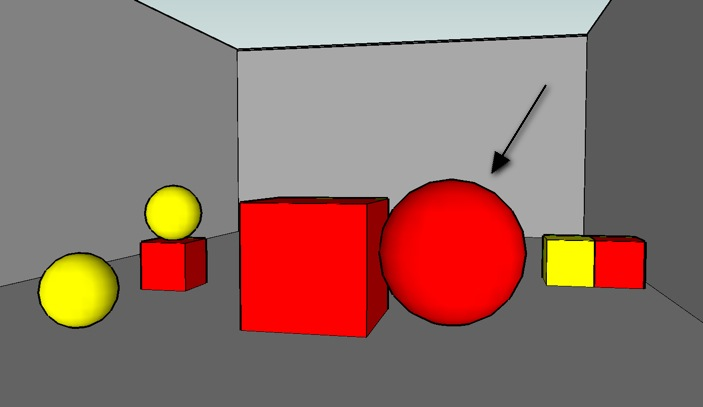
\includegraphics[width=0.6\textwidth]{images/22sinletras.jpg}
\caption{Ejemplo de contexto}
\label{GRE3D7-stimulus}
\end{figure}

Una propiedad es una caracter\'istica propia de un objeto. Por ejemplo en el Contexto \ref{GRE3D7-stimulus} el objeto se\~nalado con la flecha tiene la propiedad {\it color} con valor {\it rojo}. Por simplicidad, en el resto de la tesis vamos a decir ``tiene propiedad {\it rojo}'', cuando queremos decir que el objeto tiene la propiedad color con valor rojo. Una relaci\'on caracteriza a un objeto describiendo caracter\'isticas de otro u otros objetos.\\

%Cuando la ER no es relacional solo contiene propiedades del objeto mismo. Ej.: color, tama\~no. Note que quiz\'as el tama\~no sea con respecto a los dem\'as objetos ``la m\'as peque\~na'', pero al no incluir una descripci\'on de otro objeto no la llamamos relacional.\\
De acuerdo a las propiedades o relaciones que una expresi\'on referencial (ER) incluya, se clasifican en distintos tipos: relacional o no relacional (tambi\'en llamada proposicional), m\'inima, sobreespecificada, o subespecificada. A continuaci\'on describimos cada uno de estos tipos.\\

% en cuyo caso es una expresi\'on que no es referencial, la incluimos en nuestras propiedades porque nos va a ser \'util la definici\'on en el Cap\'itulo \ref{sec:corpus}.\\
Una ER {\it proposicional} o no relacional, incluye s\'olo propiedades intr\'insecas del objeto target. Por ejemplo en el Contexto \ref{GRE3D7-stimulus}: ``La pelota roja''. Las caracter\'isticas de ser pelota, ser roja son propias del objeto identificado.\\

Una ER es {\it relacional}, cuando adem\'as de ser proposicional, contiene relaciones con otros objetos, entonces la ER incluye las ERs de los otros objetos.  Por ejemplo en el Contexto \ref{GRE3D7-stimulus}: ``La pelota que esta a la derecha del cubo grande'', ``a la derecha de'' es una relaci\'on que necesita describir otro objeto adem\'as del target, en este caso ``el cubo grande''.\\

Se dice que una ER es {\it minimal}, cuando incluye la m\'inima cantidad de propiedades con las cuales el objeto puede ser distinguido en el contexto dado. Notar que puede haber muchas expresiones minimales. Por ejemplo en el Contexto \ref{GRE3D7-stimulus} ``La pelota roja'' es una ER minimal, como as\'i tambi\'en lo es ``La pelota grande'', ya que ambas tienen 2 propiedades, y 2 es la m\'inima cantidad de propiedades que puede tener una ER de ese objeto, para distinguirlo en ese contexto.\\

Cuando la ER contiene m\'as informaci\'on de la m\'inima necesaria para distinguirlo de los dem\'as objetos en el contexto dado, se dice que la ER es {\it sobreespecificada}. Por ejemplo: ``La pelota roja grande'' en el Contexto \ref{GRE3D7-stimulus}.\\

Una expresi\'on es {\it subespecificada} cuando no alcanza a ser una ER, ya que no se puede distinguir al objeto target de todos los objetos en el contexto. Por ejemplo: ``La pelota'' en el Contexto \ref{GRE3D7-stimulus} no alcanza para distinguir el objeto apuntado por la flecha, ya que hay otras 2 pelotas. En estos casos se debe dar otra expresi\'on o corregir la anterior agregando m\'as propiedades o relaciones. Una expresi\'on subespecificada identifica a un conjunto, no a un objeto \'unico.

\section{La tarea de generaci\'on autom\'atica de expresiones referenciales}

La generaci\'on autom\'atica de expresiones referenciales (GER), es la tarea de definir cuales pasos se deben seguir para conseguir una ER de un objeto espec\'ifico, en un contexto dado. Estos pasos definen un algoritmo de GER. \\

Los algoritmos se pueden diferenciar por la cantidad y forma de los par\'ametros que toman como input, es decir el modo en que toman por ejemplo el contexto para el cual se espera que den una expresi\'on referencial. \\

En todos los casos, la computadora necesita tener un conjunto de propiedades/relaciones para cada objeto y poder identificarlos, para ello vamos a etiquetar a los objetos con $e_1$, $e_2$, etc. como se muestra en la Figura \ref{GRE3D7-stimulus-conLetras}. En la imagen tambi\'en podemos ver que el objeto se\~nalado con la flecha es $e_5$, es el objeto target, para el cual queremos generar autom\'aticamente una expresi\'on referencial.

\begin{figure}[ht]
\centering
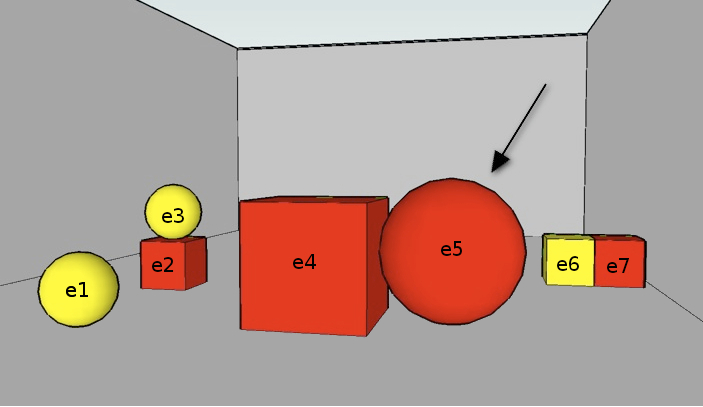
\includegraphics[width=0.6\textwidth]{images/22.jpg}
\caption{Ejemplo de contexto con objetos etiquetados}
\label{GRE3D7-stimulus-conLetras}
\end{figure}

A continuaci\'on daremos 2 ejemplos de diferentes maneras de modelar el contexto que toman como input, uno para el algoritmo Graph y otro para algoritmo de Bisimulaci\'on.\\

%El contexto que toma como input el algoritmo GRAPH \cite{graph08} el cual explicaremos en la Secci\'on \ref{graph}, para el Contexto \ref{GRE3D7-stimulus}, es un grafo dirigido y etiquetado como se muestra en Figura \ref{grafo-GRE3D7-stimulus}, el cual contiene la informaci\'on de las propiedades y relaciones de los objetos, por ejemplo podemos ver que el objeto target que es el $e_5$, tiene propiedades large, red, ball y una flecha con la etiqueta rightof $e_4$, y $e_4$ tiene propiedades large, red, cube, y una flecha hacia $e_5$ con etiqueta leftof.\\

El contexto que toma como input el algoritmo Graph \cite{graph08} el cual explicaremos en la Secci\'on \ref{graph}, para el Contexto \ref{GRE3D7-stimulus}, es un grafo dirigido y etiquetado como se muestra en Figura \ref{grafo-GRE3D7-stimulus}, el cual contiene la informaci\'on de las propiedades y relaciones de los objetos, por ejemplo podemos ver que el objeto $e_5$, tiene propiedades grande, rojo, pelota y una flecha con la etiqueta a-la-derecha-de hacia $e_4$, y $e_4$ tiene propiedades grande, rojo, cubo, y una flecha hacia $e_5$ con etiqueta a-la-izquierda-de.\\

\begin{figure}[ht]
\centering
\begin{tikzpicture}
  [
    n/.style={circle,fill,draw,inner sep=3pt,node distance=2cm},
    aArrow/.style={->, >=stealth, semithick, shorten <= 1pt, shorten >= 1pt},
  ]
 \node[n,label=above:$e_1$,label=below:{
    \relsize{-2}$\begin{array}{c}
      \nSmall\\[-3pt] 
      \nYellow \\[-3pt] 
      \nBall\end{array}$}] (a) {};
 \node[n,label=above:$e_2$,label=below:{
    \relsize{-2}$\begin{array}{c}     
      \nSmall\\[-3pt] 
      \nRed\\[-3pt] 
      \nCube\end{array}$}, right of=a] (b) {};
 \node[n,label=below:$e_3$,label=above:{
    \relsize{-2}$\begin{array}{c}
      \nTop\\[-3pt]      
      \nSmall\\[-3pt] 
      \nYellow\\[-3pt] 
      \nBall\end{array}$}, above of=b] (c) {};
 \node[n,label=right:$e_4$,label=left:{
    \relsize{-2}$\begin{array}{c}
      \nLarge\\[-3pt] 
      \nRed\\[-3pt] 
      \nCube\end{array}$}, right of=b] (d) {};
 \node[n,label=left:$e_5$,label=below:{
    \relsize{-2}$\begin{array}{c}
      \nLarge\\[-3pt] 
      \nRed\\[-3pt] 
      \nBall\end{array}$}, right of=d] (e) {};
 \node[n,label=right:$e_6$,label=left:{
    \relsize{-2}$\begin{array}{c}
      \nSmall\\[-3pt] 
      \nYellow\\[-3pt] 
      \nCube\end{array}$}, right of=e] (f) {};
 \node[n,label=left:$e_7$,label=below:{
    \relsize{-2}$\begin{array}{c}
      \nSmall\\[-3pt]
      \nRed\\[-3pt] 
      \nCube\end{array}$},  right of=f] (g) {};
 \draw [aArrow,bend right=40] (b) to node[auto,swap]{\relsize{-3}$\nBelow$} (c);
 \draw [aArrow,bend right=40] (c) to node[auto,swap]{\relsize{-3}$\nOntop$} (b);
 \draw [aArrow,bend right=40] (d) to node[auto,swap]{\relsize{-3}$\nLeftof$} (e);
 \draw [aArrow,bend right=40] (e) to node[auto,swap]{\relsize{-3}$\nRightof$} (d);
 \draw [aArrow,bend right=40] (f) to node[auto,swap]{\relsize{-3}$\nLeftof$} (g);
 \draw [aArrow,bend right=40] (g) to node[auto,swap]{\relsize{-3}$\nRightof$} (f);
 \draw[dotted] (-0.5,-1.1) rectangle (10.5,3.1);

 \end{tikzpicture}
\caption{Grafo del contexto \ref{GRE3D7-stimulus}}
\label{grafo-GRE3D7-stimulus}
\end{figure}

Para el mismo Contexto \ref{GRE3D7-stimulus-conLetras}, el input del algoritmo de Bisimulaci\'on el cual explicaremos en Secci\'on \ref{bisimulacion}, es un archivo con formato XML \footnote{XML, siglas en ingl\'es de eXtensible Markup Language ('lenguaje de marcas extensible'), es un lenguaje de marcas desarrollado por el World Wide Web Consortium (W3C) utilizado para almacenar datos en forma legible.} con la misma informaci\'on del Contexto \ref{input-bisimulacion}. En este caso se representan las propiedades como relaciones a un objeto ficticio, terminal {\it c}, creado para modelar propiedades y relaciones, como relaciones, como veremos luego esto va a servir para dar prioridad a las relaciones en algunos casos. En el XML podemos ver que todos los objetos tienen ``id'' que es el identificador, salvo el objeto target $e_5$ el cual tiene {\it refer-to} en vez de {\it id}. Con la etiqueta ``rel'', identificamos las relaciones y con la etiqueta ``to'' con que objeto esta relacionado. El target tiene relaciones con c (grande, rojo, pelota) y con $e_4$ a-la-derecha-de.  
%\'Este tiene las relaciones con c (large, red, ball) y con $e_4$ rightof.  
\textcolor{blue}{aca tengo problemas en verbatim para escribir la enie de pequeino}
\label{input-bisimulacion}

%\include{xml}

\begin{verbatim}
<?xml version="1.0"?>
<problem id="e1">c
  <individual id="e1">
    <related rel="pequeno" to="c" />
    <related rel="amarillo" to="c" />
    <related rel="pelota" to="c" />
  </individual>
  ...
  <individual id="e4">
    <related rel="cubo" to="c" />
    <related rel="rojo" to="c" />
    <related rel="grande" to="c" />
    <related rel="a-la-izquierda-de" to="e5" />
  </individual>
  <individual refer-to="e5">
    <related rel="grande" to="c"/>
    <related rel="pelota" to="c" />
    <related rel="rojo" to="c" />
    <related rel="a-la-derecha-de" to="e4" />
  </individual>
  ...
  <individual id="c">
    <related rel="terminal" to="c" />
  </individual> 
</problem>
\end{verbatim}
%\label{input-bisimulacion}
%\begin{verbatim}
%<?xml version="1.0"?>
%<problem id="e1">c
  %<individual id="e1">
    %<related rel="small" to="c" />
    %<related rel="yellow" to="c" />
    %<related rel="ball" to="c" />
  %</individual>
  %...
  %<individual id="e4">
    %<related rel="cube" to="c" />
    %<related rel="red" to="c" />
    %<related rel="large" to="c" />
    %<related rel="left-of" to="e5" />
  %</individual>
  %<individual refer-to="e5">
    %<related rel="large" to="c"/>
    %<related rel="ball" to="c" />
    %<related rel="red" to="c" />
    %<related rel="right-of" to="e4" />
  %</individual>
  %...
  %<individual id="c">
    %<related rel="terminal" to="c" />
  %</individual> 
%</problem>
%\end{verbatim}
%Saque para que no quede tan largo
%<individual id="e6">
    %<related rel="small" to="c" />
    %<related rel="cube" to="c" />
    %<related rel="yellow" to="c" />
    %<related rel="left-of" to="e7" />
  %</individual>
  %<individual id="e7">
    %<related rel="small" to="c" />
    %<related rel="cube" to="c" />
    %<related rel="red" to="c" />
    %<related rel="right-of" to="e6" />
  %</individual>

%<individual id="e2">
%    <related rel="cube" to="c" />
%    <related rel="red" to="c" />
%    <related rel="small" to="c" />
%    <related rel="bellow" to="e3" />
%  </individual>
%  <individual id="e3">
%    <related rel="ball" to="c" />
%    <related rel="yellow" to="c" />
%    <related rel="small" to="c" />
%    <related rel="on-top" to="e2" />
%  </individual>
Los algoritmos tambi\'en se pueden diferenciar por la clase de ER que pueden generar, a continuaci\'on explicaremos los distintos tipos de algoritmos de GER. 

\section{Tipos de algoritmos de GER}

Un algoritmo para la generaci\'on autom\'atica de expresiones referenciales  puede ser: determin\'{i}stico o no-determin\'{i}stico, relacional o proposicional, incluir negaciones o no, identificar plurales o s\'olo singulares,
 %usar disyunciones y conjunciones, o s\'olo conjunciones, 
generar ER sobreespecificadas o minimales.  A continuaci\'on se describen cada uno de esos tipos.\\

Un algoritmo es {\it determin\'{i}stico} si dado un input (un contexto y un objeto target), da siempre la misma ER de salida. En cambio un algoritmo es {\it no-determin\'{i}stico} si es posible que d\'e distintas salidas para el mismo input, en distintas ejecuciones. En general las personas generan expresiones referenciales de forma no determin\'istica, por lo tanto los algoritmos no determin\'isticos simulan el comportamiento de distintas personas, o incluso el de la misma persona en distintos momentos. Por ejemplo ser\'ia no determin\'istico si para el Contexto \ref{GRE3D7-stimulus-conLetras} una vez da ``La pelota roja'' y en otra ejecuci\'on ``La pelota grande''.\\

Un algoritmo es {\it proposicional}, cuando las ER que genera contienen solo atributos del target, es decir no contiene relaciones con otros atributos ni ER de otros objetos.  Por ejemplo para el Contexto \ref{GRE3D7-stimulus-conLetras} una vez da ``La pelota roja''.\\

Un algoritmo es {\it relacional} si adem\'as de generar ER proposicionales genera ER relacionales, en cuyo caso adem\'as de generar las relaciones correspondientes deber\'a generar ERs para el o los objetos relacionados. Por ejemplo para el Contexto \ref{GRE3D7-stimulus-conLetras} la ER ``La pelota roja a la derecha del cubo grande''. En este caso ``el cubo grande'' es una expresi\'on referencial que se tuvo que dar como consecuencia de incluir la relaci\'on ``a la derecha de''.\\

En algunos contextos cuando el target es el \'unico que no tiene una propiedad por ejemplo, ser\'ia \'util un algoritmo que incluya {\it negaciones}. Por ejemplo para el Contexto \ref{GRE3D7-stimulus-conLetras}, ``La \'unica pelota que no es peque\~na''.\\

Un algoritmo puede generar ER para {\it plurales}, es decir dar ER para varios targets en el contexto considerado. Por ejemplo para el Contexto \ref{plurales}, ``Los objetos grandes''. En este caso el target no es \'unico, sino un conjunto de objetos. \\

\begin{figure}[ht]
\centering
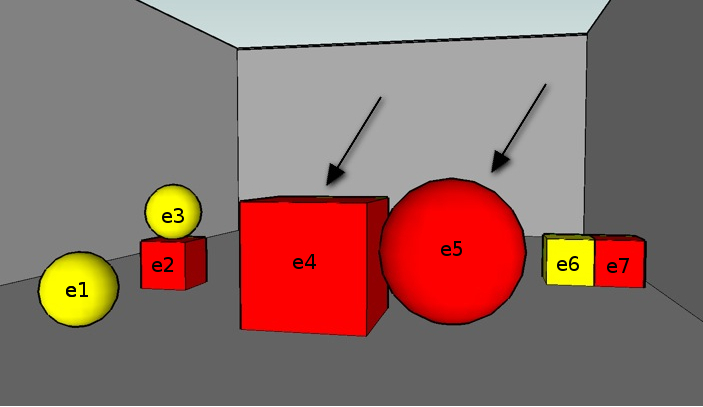
\includegraphics[width=0.6\textwidth]{images/22-plural.jpg}
\caption{Ejemplo de contexto con 2 targets}
\label{plurales}
\end{figure}
%esto lo saque porque confunde aca... me parece que todavia no hay que hablar de esto, es muy de logica
%Los algoritmos tambi\'en se pueden diferenciar en los conectores que permiten si usan conjunciones, disyunciones o ambas.\\

Un algoritmo que genera ER {\it minimales}, es un algoritmo que da ER que contienen la m\'inima cantidad de propiedades o relaciones que se necesitan para distinguir al target.  Por ejemplo para el Contexto \ref{GRE3D7-stimulus-conLetras} ``La pelota grande''.\\

La {\it sobreespecificaci\'on} es la caracter\'istica de dar m\'as atributos o relaciones de las necesarias para identificar al objeto target. Por ejemplo para el Contexto \ref{GRE3D7-stimulus-conLetras} la ER ``La pelota roja, grande que esta a la derecha del cubo rojo grande'' es una ER sobreespecificada.\\

%no se si dejar esto...
%Un algoritmo que hace backtraking, es el que luego de incluir una propiedad o relaci\'on puede deshacer esa inclusi\'on volviendo a un estado anterior, es decir, decidir no incluirla.\\

\section{Algoritmos importantes en el \'area}
%interesante...
%https://www.abdn.ac.uk/ncs/departments/computing-science/tunabibl-495.php

En esta secci\'on vamos a hablar de los algoritmos de generaci\'on autom\'atica de expresiones referenciales, empezando por el algoritmo Full Brevity, el algoritmo de heur\'istica Greedy, siguiendo con el algoritmo Incremental, Graph, algoritmo Relacional y por \'ultimo Bisimulaci\'on.  \\

%http://citeseerx.ist.psu.edu/viewdoc/download?doi=10.1.1.227.8284&rep=rep1&type=pdf

%REG can be traced back to the earliest days of Natural Language Processing; Winograd
%(1972)  (Section  8.3.3,  Naming  Objects  and  Events),  for  example,  sketches  a  primitive
%“incremental” REG algorithm, used in his SHRDLU program. In the 1980s, researchers
%such as Appelt and Kronfeld set themselves the ambitious task of modelling the human
%capacity for producing and understanding referring expressions in programs such as
%KAMP and BERTRAND (Appelt 1985; Appelt and Kronfeld 1987; Kronfeld 1990). They
%argued that referring expressions should be studied as part of a larger speech act. KAMP
%(Appelt  1985),  for  example,  was  conceived  as  a  general  utterance  planning  system,
%building  on  Cohen  and  Levesque’s  (1985)  formal  speech  act  theory.

%REG  task  is  now  defined  by  Dale  and  Reiter  (1995)  through  what  may  be
%called identification of the target: given a target (or referent) object r 2 D , find a set of attribute–value  pairs L
%whose  conjunction  is  true  of  the  target  but  not  of  any  of  the
%distractors (i.e., D

%Full  Brevity  and  Greedy  Heuristic.
El algoritmo {\it Full Brevity} \cite{Dale:1989:CUR:981623.981632} genera la descripci\'on m\'as corta que identifica al target. Para hacerlo, 
busca si hay una propiedad del target que no sea propiedad de ning\'un distractor. Si no hay chequea todas las posibles combinaciones de 2 propiedades, si no la hay, busca de a 3 y as\'i sucesivamente.\\

El problema es que encontrar la descripci\'on m\'as corta es de alta complejidad, se observ\'o que las personas dan expresiones que no son minimales, esto fue confirmado por estudios psycoling\"uisticos (\cite{Olson1970LangAndThought};  \cite{Sonnenschein1984}; \cite{Pechmann1989}; \cite{Engelhardt2006}).\\

Una aproximaci\'on a Full Brevity es el algoritmo de heur\'istica {\it Greedy}, el cual iterativamente selecciona la propiedad que elimina m\'as distractores y argumentan que la propiedad seleccionada tiene el m\'as alto poder discriminativo en esa etapa. Como resultado no siempre genera expresiones referenciales m\'inimas.\\

%which  iteratively  selects  the  property  which  rules  out  most  of  the  distractors
%not  previously  ruled  out,  incrementally  augmenting  the  description  based  on  what
%property has most discriminatory power at each stage (as a result, it does not always
%generate  descriptions  of  minimal  size). 
El algoritmo de heur\'istica Greedy es m\'as eficiente que el Full Brevity, pero pronto fue superado por el algoritmo {\it Incremental} y sus sucesores \cite{C92-1038}; \cite{Dale95computationalinterpretations}. El algoritmo Incremental fue y sigue siendo uno de los algoritmos m\'as importantes del \'area, lo explicamos a continuaci\'on. 
% The  Greedy  Heuristic  algorithm  is  a  more
%efficient  algorithm  than  the  Full  Brevity  one,  but  it  was  soon  eclipsed  by  another
%algorithm    which  turned  out  to  be  the
%most influential algorithm of the pre-2000 era. It is this later algorithm that came to be
%known as``the'' Incremental Algorithm (IA).

%\subsection{GREEDY}

%El algoritmo GREEDY de Dale~\cite{dale89} busca sobre todo el conjunto de propiedades del target y elije el subconjunto m\'as chico posible que identifica un\'{i}vocamente al objeto target entre los distractores en la escena considerada como se muestra en el siguiente algoritmo.\\

%\begin{figure}[ht]
%\begin{center}
%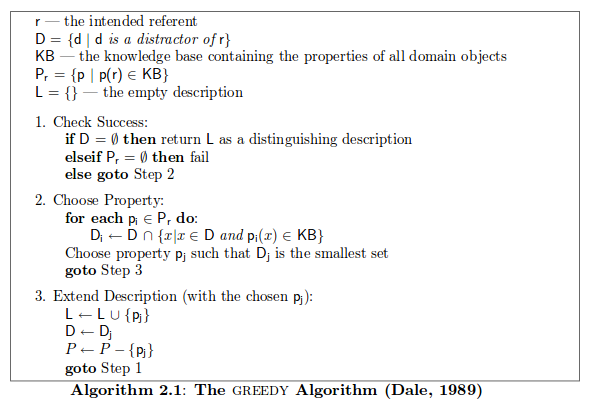
\includegraphics[width=8.5cm]{figures/greedy.png}\\[0pt]
%\caption{Interface del experimento}
%\label{fig-greedy}
%\end{center}
%\end{figure}

%r - el objeto target\\
%D = \{d|d es un distractor de r\}\\
%KB - la base de conocimiento que contiene las propiedades de todos los objetos\\
%$P_{r}$ = $\{p|p(r) \in KB\}$\\
%L = $\{\}$ - la descripci\'on vac\'{i}a\\
%\\
%1. Chequea \'exito:\\
%    \textbf{if} D = $\emptyset$ \textbf{then} return L como una ER que distingue al target r
%    \textbf{elseif} $P_{r}$ = $\emptyset$ \textbf{then} fail
%    
%\textbf{else goto} Paso 2 \\
%\\
%2. Elegir Propiedad:
% \textbf{for each} $p_{i}$ $\in$ $P_{r}$ \textbf{do}:
%    $D_{i}$ $\leftarrow$ D$\cap$ \{x|x $\in$ D and $p_{i}$ (x) $\in$ KB\}
%    Elegir la propiedad $p_{j}$ tal que $D_{j}$ es el conjunto m\'as chico (es decir la que elimina m\'as distractores) \textbf{goto} Paso 3\\
%\\    
%3. Agregar $p_{j}$ a la descripci\'on actual\\
%L $\leftarrow$ L $\cup$ \{$p_{j}$\}\\
%D $\leftarrow$ $D_{j}$\\
%P $\leftarrow$ P -\{$p_{j}$\}\\
%\textbf{goto} Paso 1\\



%%Dado un dominio D que contiene un target referente r y un conjunto de distractores, una base de conocimiento KB que contiene las propiedades de los objetos.
%%Un conjunto de propiedades verdaderas para r, y una descripcion L inicialmente vac\'{i}a.

%Este algoritmo es de orden NP-complete

\subsection{Incremental}

%A continuaci\'on se describe el algoritmo Incremental de Dale \& Reiter el cual esta basado en el algoritmo GREEDY (el cual hac\'ia una b\'usqueda exaustiva y eleg\'ia la propiedad que m\'as distractores eliminaba en cada paso) pero \'este reduce la complejidad del algoritmo Greedy cambiando que en vez de chequear cual propiedad es la que elimina m\'as distractores, eligiendo la que sigue en la lista de propiedades ordenada seg\'un preferencia y que elimina al menos un distractor. Este algoritmo es de orden polinomial. Este algoritmo produce expresiones referenciales que pueden estar sobreespecificadas.\\

\textcolor{blue}{error entorno matematico, pero no entiendo porque, y no puedo hacer que diga algoritmo en vez de algorithm}

%\begin{figure}
\small
\begin{center}
%\centering
\begin{algorithm}[H]

\dontprintsemicolon

\captionsetup[algorithm]{name=Algoritmo}
\caption{Incremental\label{algo:incremental}}
%\caption{Incremental}\label{algo:incremental}
\KwIn{\footnotesize \{r, D, Pref\} r es el target, D es el dominio, Pref lista de preferencia de propiedades ordenadas}
\KwOut{\footnotesize L  - Descripci\'on de salida}

$\ L \leftarrow \emptyset $ \tcp*[f]{\footnotesize Inicialmente es vac\'io}\\
$\ C \leftarrow D - \{r\} $ \tcp*[f]{\footnotesize C es el conjunto de todos los objetos menos r }\\


\For{\em $A_{i} \in Pref$ }{
	$V = Value(r,A_{i})$ \tcp*[f]{\footnotesize V es el valor de la propiedad $A_{i}$ para r }\\
	\If(\tcp*[f]{\footnotesize Si elimina alg\'un distractor}){\em $C \cap RulesOut(\[A_{i}\],V) \neq \emptyset $}
	{
    $\ L \leftarrow L \cup \{A_{i},V\} $  \tcp*[f]{\footnotesize Agrega la propiedad $A_{i}$ a L }\\
    $\ C \leftarrow C - RulesOut(\[A_{i}\],V) $  \tcp*[f]{\footnotesize Actualiza C sacando los objetos que no tienen V en $A_{i}$} 
    }
    \If(\tcp*[f]{\footnotesize Si no quedan distractores}){\em $C = \emptyset $}
	  {
     Return L  
    }
  }
Return Fallo
\end{algorithm}
\end{center}
%\end{figure}



Como podemos ver en \ref{algo:incremental} el input de este algoritmo es el objeto target que queremos identificar {\it r}, D, el dominio, y Pref una lista ordenada de preferencia de propiedades.\\
En {\it Paso 1} se asigna a L la descripci\'on vac\'{i}a, al finalizar la ejecuci\'on, L tendr\'a el conjunto de propiedades con los cuales identificaremos a r, es decir una expresi\'on referencial de r. 
Se le asigna a C el conjunto de distractores de r (todos los objetos menos r), en {\it Paso 2}.\\

La idea del algoritmo es ir eliminando distractores, por eso, en el {\it Paso 3} recorre las propiedades de r. En {\it Paso 4} le asigna a V el valor que tiene el target para la propiedad $A_{i}$

$RulesOut(A_{i},V)$ devuelve el conjunto de objetos que tienen diferente valor para la propiedad $A_{i}$ que el que tiene el objeto target.

Si hay objetos en C que tengan diferente valor de $A_{i}$ que el target, se agrega la propiedad a la descripci\'on actual L en {\it Paso 6}, y se actualiza $C$ sacando los objetos que no tienen V en $A_{i}$. 

Luego en {\it Paso 8} si C es $\emptyset$ (si no hay m\'as distractores) devolvemos L, como el conjunto de propiedades que identifican a r.

Vamos a ejemplificar la corrida del algoritmo con el ejemplo de Contexto \ref{GRE3D7-stimulus-conLetras}, y supongamos que la lista ordenada de propiedades es esta [ tipo, color, tama\~no ]. D inicialmente es \{$e_{1}$,$e_{2}$,$e_{3}$,$e_{4}$,$e_{5}$,$e_{6}$,$e_{7}$\}
Al iniciar a L le asigna $\emptyset$ y a C \{$e_{1}$,$e_{2}$,$e_{3}$,$e_{4}$,$e_{6}$,$e_{7}$\}, luego comienza a recorrer la lista de propiedades, la primer propiedad es ``tipo'', el valor del target para tipo es {\it pelota}, entonces en {\it Paso 6}, pregunta si hay objetos que tengan tipo con valor distinto de pelota, y hay, ellos son \{$e_{2}$,$e_{4}$,$e_{6}$,$e_{7}$\}, entonces le asigna a C \{$e_{1}$,$e_{3}$\}, es decir solo las pelotas. En {\it Paso 10} pregunta si C es vac\'io, no lo es, por lo tanto continua con la siguiente propiedad, en este caso ``color'', el valor de color para el target es {\it rojo}, agrega {\it rojo} a L, y actualiza C con $\emptyset$ porque tanto $e_{1}$ como $e_{3}$ son amarillos, en {\it Paso 10} pregunta si C es vac\'io, y si lo es, por lo tanto devuelve \{pelota, rojo\}.


%Intuitivamente, si la primer propiedad tipo y el valor de tipo para el target es ``pelota'', nos quedamos con todos los objetos pelota.\\

%\textcolor{blue}{Un poco mas de historia, no se a donde poner...Theune and Krahmer proposed an extension that allows the generation of subsequent reference with the ia taking into account the discourse salience of the target referent (Krahmer and Theune, 1998; Theune, 2000; Krahmer and Theune, 2002), and a second one which allows the ia to produce referring expressions that
%contain binary relations to other objects (Theune, 2000; Krahmer and Theune, 2002). I will return to their relational extension in Section 2.3. Theune and Krahmer's approach works by assigning a salience score to all objects according to the
%focus/topic distinction by Hajicova (1993) and Centering Theory (Grosz et al., 1995). They alter the success criterion of the algorithm and only let it stop when here is no distractor left that is as or more salient than the target referent.
%Not all properties are the same. The qualitative diferences that exist between diferent properties were first discussed in the
%reg literature by van Deemter (2000, 2006). He pointed out that the appropriateness of
%vague orgradable properties such as small and large is dependent on the context in which they are used, while,
%for example, the colour of an object is absolute. Consider two descriptions in a domain of animals... (van Deemter, 2002), van Deemter considered the ia's logical completeness in terms of the Boolean operators of negation and disjunction. He extended it to
%be able to generate referring expressions that contain negated properties, such as Example (2.3), and descriptions of sets of objects, such as Example (2.4), or even (2.5), which contains a logical disjunction of properties. His algorithm proceeds
%in stages, trying longer and longer disjunctions of properties, if atomic properties
%and shorter disjunctions did not suffice to distinguish the target set.. he work on reference to sets was taken further by Gatt and van Deemter (2005, 2006), who have presented the most mature algorithms in this space to
%date. They used a similar procedure to the ia in that their algorithms are based
%on incremental processing of a preference order of properties. Their algorithms
%add a lot of complex machinery to the basic procedure to ensure that properties
%are chosen in a way that maximises coherence within the set of objects described
%by the referring expressions. For example, their approach will attempt to use
%properties of the same type for all the referents of a set. So, it would produce
%descriptions such as Examples 
Luego se propusieron extensiones del algoritmo Incremental, por ejemplo 
Theune y Krahmer propusieron una extensi\'on que permite la generaci\'on de referencia teniendo en cuenta la prominencia discurso del target (\cite{Krahmer:2010:EMN:1880370}; \cite{krahmer-theune:2002a};), y un segundo algoritmo que permite producir expresiones referenciales que contienen relaciones con otros objetos. El enfoque Theune y de Krahmer funciona asignando una puntuaci\'on de relevancia a todos los objetos de acuerdo con el enfoque / tema distinci\'on por \cite{hajicova-1993} y la teor\'ia de centrado \cite{Grosz:1995:CFM:211190.211198}. Alteran el criterio de \'exito del algoritmo y s\'olo permiten que se detenga cuando hay un distractor que es tanto o m\'as relevante que el target.
No todas las propiedades tienen la misma relevancia. Las diferencias cualitativas que existen entre diferentes propiedades se discutieron por primera vez en la literatura GER por van Deemter (2000, 2006). Se\~nal\'o que la conveniencia de otras propiedades sobre las
propiedades vagas como peque\~no y grande dependen del contexto en el que se utilizan, mientras que, por ejemplo, el color de un objeto es absoluta. 
%Considere dos descripciones de un dominio de los animales ... (van Deemter, 2002), van Deemter considera integridad l\'ogica del ia en t\'erminos de los operadores booleanos de negaci\'on y disyunci\'on. \'el la extendi\'o a
%ser capaz de generar expresiones referenciales que contienen propiedades, tales como Ejemplo (2.3) negado, y las descripciones de conjuntos de objetos, tales como Ejemplo (2.4), o incluso (2,5), que contiene una disyunci\'on l\'ogica de propiedades. Sus algoritmo procede
%en etapas, tratando m\'as y disyunciones m\'as largos de propiedades, si las propiedades at\'omicas
%y disyunciones m\'as cortos no son suficientes para distinguir el conjunto target .. que funciona en referencia a conjuntos fue tomada adem\'as por Gatt y van Deemter (2005, 2006), que han presentado los algoritmos m\'as maduros a la fecha. Utilizaron un procedimiento similar al de las otras cosas en que sus algoritmos se basan en el procesamiento incremental de un orden de preferencia de las propiedades. Sus algoritmos agregan una gran cantidad de maquinaria compleja para el procedimiento b\'asico para asegurar que las propiedades
%se eligen de manera que maximiza la coherencia dentro del conjunto de objetos descritos por las expresiones referenciales. Por ejemplo, su enfoque intentar\'a utilizar propiedades del mismo tipo para todos los referentes de un conjunto. As\'i, ser\'ia producir
%descripciones tales como ejemplos
%(2.6) or (2.7) rather than Example (2.8) or.. 


%Theune y Krahmer propusieron una extensi\'on que permite la generaci\'on de referencia con la subsiguiente ia teniendo en cuenta la prominencia discurso del referente objetivo (Krahmer y Theune, 1998; Theune, 2000; Krahmer y Theune, 2002), y un segundo uno que permite la IA para producir expresiones referenciales que contener relaciones binarias a otros objetos (Theune, 2000; Krahmer y Theune, 2002). Voy a volver a su extensi\'on relacional en la Secci\'on 2.3. Enfoque Theune y de Krahmer funciona asignando una puntuaci\'on de relevancia a todos los objetos de acuerdo con la enfoque / tema distinci\'on por Hajicova (1993) y el centrado Theory (Grosz et al., 1995). Alteran el criterio de \'exito del algoritmo y s\'olo permiten que se detenga cuando aqu\'i hay izquierda distractor que es tan o m\'as relevante que el referente de destino.
%No todas las propiedades son las mismas. Las Diferencias cualitativas que existen entre diferentes propiedades se discutieron por primera vez en la literatura reg por van Deemter (2000, 2006). Se\~nal\'o que la conveniencia de propiedades orgradable vagos como peque\~nos y grandes depende del contexto en el que se utilizan, mientras que, Por ejemplo, el color de un objeto es absoluta. Considere dos descripciones de un dominio de los animales ... (van Deemter, 2002), van Deemter considera integridad l\'ogica del ia en t\'erminos de los operadores booleanos de negaci\'on y disyunci\'on. \'el la extendi\'o a ser capaz de generar expresiones que se refieren que contienen propiedades, tales como Ejemplo (2.3) negado, y las descripciones de conjuntos de objetos, tales como Ejemplo (2.4), o incluso (2,5), que contiene una disyunci\'on l\'ogica de propiedades. Sus algoritmo procede en etapas, tratando m\'as y disyunciones m\'as largos de propiedades, si las propiedades at\'omicas y disyunciones m\'as cortos no son suficientes para distinguir el conjunto de destino .. que funciona en referencia a conjuntos fue tomada adem\'as por Gatt y van Deemter (2005, 2006), que han presentado los algoritmos m\'as maduros en este espacio para la fecha. Utilizaron un procedimiento similar al de las otras cosas en que sus algoritmos se basan en el procesamiento incremental de un orden de preferencia de las propiedades. Sus algoritmos agregar una gran cantidad de maquinaria compleja para el procedimiento b\'asico para asegurar que las propiedades se eligen de manera que maximiza la coherencia dentro del conjunto de objetos descritos por las expresiones que se refieren. Por ejemplo, su enfoque intentar\'a utilizar propiedades del mismo tipo para todos los referentes de un conjunto. As\'i, ser\'ia producir Ejemplos descripciones tales como (2,6) o (2,7) en lugar de Ejemplo (2.8) o ..


\subsection{Algoritmo de b\'usqueda en Grafo}
\label{graph}
%Un grafo es un conjunto de objetos llamados v\'ertices o nodos unidos por enlaces llamadas aristas o arcos, que permiten representar relaciones binarias entre elementos de un conjunto. \\

Un grafo G es un par ordenado $G=(V,E)$, donde:
\begin{itemize}
   \item V es un conjunto de v\'ertices o nodos, y
    \item E es un conjunto de aristas o arcos, que relacionan estos nodos.

%\item Se llama orden del grafo G a su n\'umero de v\'ertices, $|V|$.

%\item El grado de un v\'ertice o nodo $v \in V$ es igual al n\'umero de arcos que lo tienen como extremo.

%\item Un bucle es una arista que relaciona al mismo nodo; es decir, una arista donde el nodo inicial y el nodo final coinciden.

%\item Dos o m\'as aristas son paralelas si relacionan el mismo par de v\'ertices.

%\item Un grafo puede ser dirigido o no, etiquetado o no.
\end{itemize}
%T\'{i}picamente, un grafo se representa gr\'aficamente como un conjunto de puntos (v\'ertices o nodos) unidos por l\'{i}neas (aristas).

Los grafos han sido muy estudiados, pr\'acticamente cualquier problema puede ser expresado como un problema de grafos, y aplicar algoritmos de b\'usqueda ya estudiados.

El algoritmo Graph de \cite{Krahmer:2003} propone ver la obtenci\'on de expresiones referenciales como un problema de grafos, el contexto que incluye al target y los distractores es representado como un grafo. \\

Cada objeto de la escena se modela como un v\'ertice en el grafo. Las propiedades at\'omicas como color, tipo o tama\~no se representan como un bucle en el correspondiente nodo. Est\'an etiquetados con los nombres de las propiedades y los valores que el objeto en cuesti\'on tiene para estas propiedades. \\

Las relaciones binarias entre objetos, por ejemplo abajo-de, arriba-de se modelan como aristas entre los nodos correspondientes.\\

%La base de conocimiento que incluye al target ahora esta expresada como los v\'ertices, las aristas y las etiquetas del grafo.\\

%Krahmer et al.'s (2003) reformularon la tarea de seleccionar las propiedades y relaciones que contendr\'a una expresi\'on referencial como un problema de teor\'ia de grafos.

Para generar una descripci\'on distintiva, el algoritmo busca un subgrafo del grafo original que identifica al target un\'{i}vocamente, le llama grafo distintivo.\\% (distinguishing graph).\\

Comenzando con el subgrafo que contiene un solo v\'ertice, que representa al target, se realiza una b\'usqueda exhaustiva, pero comenzando a lo ancho. Utiliza una heur\'{i}stica basada en el costo (costo de incluir propiedades, relaciones) para podar el espacio de b\'usqueda. Y da el grafo de menor costo. \\


%esto no se entiende nada
%Informalmente, un subgrafo refiere al target si y s\'olo si puede ser
%`Colocado sobre el gr\'afico de dominio de tal manera que el v\'ertice que representa subgrafo
%del objeto target se puede `coloca sobre 'el v\'ertice del objetivo en el gr\'afico de dominio,
%y cada uno de los bordes marcados en el subgrafo puede ser `coloca sobre 'un correspondiente
%borde en el gr\'afico de dominio con la misma etiqueta y el mismo sentido. Por otra parte,
%un subgrafo distingue al target un\'ivocamente si y s\'olo si se puede `colocarlo sobre grafo original' y es exactamente el
%v\'ertice target. La noci\'on informal de un gr\'afico que se coloca sobre otro corresponde al concepto te\'orico matem\'atico de isomorfismo de grafos.

En teor\'{i}a de grafos, un isomorfismo entre dos grafos G y H es una biyecci\'on f entre los conjuntos de sus v\'ertices $f:V(G) \rightarrow V(H)$ que preserva la relaci\'on de adyacencia. Es decir, cualquier par de v\'ertices u y v de G son adyacentes si y solo si lo son sus im\'agenes, $f(u)$ y $f(v)$, en H.\\

%\textcolor{blue}{aca quiero poner un ejemplo que muestre una imagen y el modelo como grafo}

La funci\'on de costo esta definida sobre las aristas y v\'ertices del grafo dominio. El costo de un subgrafo se define como la suma sobre todas las aristas y v\'ertices que contiene el grafo.\\
El algoritmo de b\'usqueda garantiza encontrar el subgrafo de menor costo que representa al target.\\

La funci\'on de costo es usada para podar las ramas del \'arbol de b\'usqueda cuando estas se hacen m\'as costosas que el grafo de menor costo encontrado hasta el momento. Esta funci\'on hace que se prefieran propiedades sobre otras que tienen mayor costo.

\textcolor{blue}{aca quiero agregar ejemplo, no me gusta como quedo esta parte}


\subsection{Bisimulaci\'on}
\label{bisimulacion}

%Este algoritmo fue propuesto por %\cite{}

La idea es transformar el problema de GER al problema de computar una f\'ormula de l\'ogicas para la descripci\'on (DL) cuya extensi\'on sea el elemento target (o los elementos targets, en el caso de querer dar una ER para plurales aprovechando que una f\'ormula describe un conjunto que puede contener m\'as de un elemento).\\

A continuaci\'on daremos una introducci\'on a las l\'ogicas para la descripci\'on \alc y \el.\\

\emph{F\'ormulas} (o \emph{conceptos}) $\varphi$ de $\alc$ son generadas por la siguiente gram\'atica:
$$
\varphi,\varphi' ::= \top \mid p \mid \neg \varphi \mid \varphi \sqcap \varphi'
\mid \exists R. \varphi
$$
donde $p$ es el conjunto de los s\'imbolos proposicionales \prop y $R$ es el de los s\'imbolos relacionales \rel. $\el$ es la parte sin negaci\'on de $\alc$.\\

Las f\'ormulas de ambos $\alc$ y $\el$ son interpretadas en modelos relacionales de primer orden $\gM = (\Delta,\interp{\cdot})$ donde
$\Delta$ es un conjunto no vac\'io y $\interp{\cdot}$ es una funci\'on de interpretaci\'on tal que:
$$
\begin{array}{ccl}
\interp{p} & \subseteq & \Delta  \mbox{ para $p \in \prop$}\\
\interp{R} & \subseteq & \Delta \times \Delta  \mbox{ para $R \in \rel$}\\
\interp{\neg \varphi} & = & \Delta - \interp{\varphi}\\
\interp{\varphi \sqcap \varphi'} & = & \interp{\varphi} \cap \interp{\varphi'}\\
\interp{\exists R.\varphi} & = & \{i \mid \mbox{para alg\'un } i', (i,i') \in \interp{R}\\
& & \mbox{ e } i' \in \interp{\varphi} \}.\\
\end{array}
$$

\begin{figure}[ht]
\begin{center}
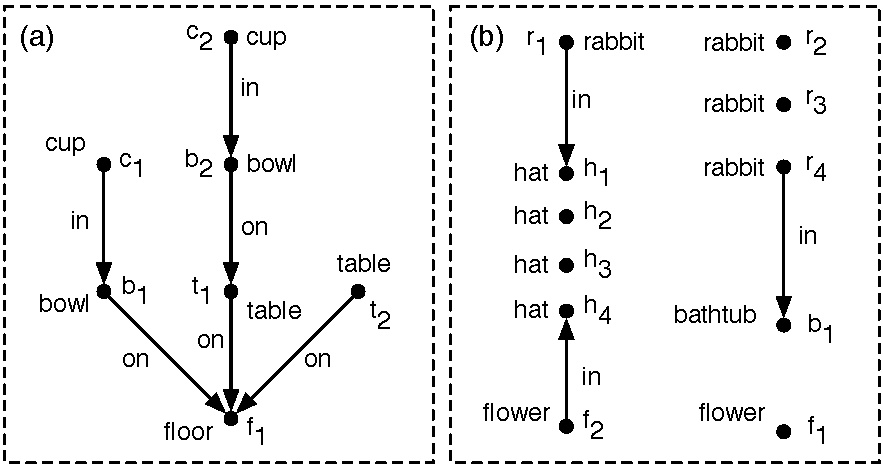
\includegraphics[width=8.5cm]{figures/pic-dale-haddock.pdf}\\[0pt]
\caption{}
\label{fig:dale-haddock}
\end{center}
\end{figure}


Cada f\'ormula de una descripci\'on l\'ogica denota un conjunto de objetos del dominio; por lo tanto podemos usar tales f\'ormulas para describir conjuntos. Por ejemplo en el modelo de la Figura.~\ref{fig:dale-haddock}b, la f\'ormula
$\mathsf{flower}$ denota el conjunto $\{f_1,f_2\}$; La f\'ormula
$\mathsf{flower} \sqcap \exists \mathsf{in}.\mathsf{hat}$ denota
$\{f_2\}$; y la f\'ormula $\mathsf{flower} \sqcap \neg
\exists \mathsf{in}.\mathsf{hat}$ denota $\{f_1\}$.\\

\textcolor{blue}{no se si dejar este ejemplo, o cambiarlo por uno es espa\~nol}

Hay muchas otras l\'ogicas de descripci\'on (DL) en la literatura por ejemplo 

$\mathcal{CL}$ (\el\ sin el cuantificador existencial, es decir solo conjunciones at\'omicas); $\mathcal{PL}$ (\alc\ l\'ogica propocisional); y
$\mathcal{ELU}_{(\neg)}$ (\el\ m\'as disjunci\'on y negaci\'on at\'omica).\\

Usaremos una noci\'on de preservaci\'on de f\'ormulas que llamaremos
\emph{similaridad}. Para cualquier DL $\gL$, diremos que un individual $i$ es \emph{\gL-similar} a $i'$ en un modelo dado $\gM$
si para cualquier f\'ormula $\varphi \in \gL$ tal que $i \in
\interp{\varphi}$, tambi\'en tenemos que $i' \in \interp{\varphi}$.\\
Equivalentemente, no hay $\gL$-f\'ormula que se mantenga para $i$ pero no para
$i'$.  Diremos que el \emph{\gL-conjunto de similaridad} de alg\'un individual
$i$ es el conjunto de todos los individuales a los cuales $i$ es \gL-similar.\\

Notar que la similaridad no es necesariamente una relaci\'on sim\'etrica: Por ejemplo:$f_1$ es \el-similar a $f_2$ en
Figura~\ref{fig:dale-haddock}b, pero $f_2$ no es \el-similar a $f_1$
(satisface la f\'ormula $\exists \mathsf{in}.\mathsf{hat}$ y $f_1$
no la satisface).  De todas maneras, \alc-similaridad es una relaci\'on sim\'etrica porque
el languaje contiene negaci\'on; y en consecuencia, $f_1$ no es \alc-similar
a $f_2$ porque este tampoco satisface $\neg \exists
\mathsf{in}.\mathsf{hat}$.  Porque \alc\ es m\'as expresivo que \el,
esto es, para alg\'un individual $a$ es posible ser \el-similar pero
no \alc-similar a alg\'un individual $b$, pero no viceversa.\\



%\textcolor{blue}{SACAR ESTO... poner quizas en la introduccion o en primer capitulo. Las ER que involucran relaciones han recibido m\'as atenci\'on recientemente;
%especialmente en el contexto de las expresiones referenciales espaciales en generaci\'on (por ejemplo,~\cite{kelleher06:increm}), donde es particularmente natural utilizar expresiones que implican relaciones espaciales, tales como ``la pelota en la parte superior del cubo''. Sin embargo, el algoritmo cl\'asico por~\cite{dale91:gener} ha demostrado ser incapaz de generar ER satisfactorias en la pr\'actica (v\'ease el an\'alisis sobre el~\emph{cabinet corpus} en~\cite{viethen06:_algor_for_gener_refer_expres}). Adem\'as, el Dale y Haddock algoritmo y muchos de sus sucesores (tales como~\cite{kelleher06:increm}) son vulnerables a el problema de la \emph{regresi\'on infinita}, donde el algoritmo entra en un bucle infinito, saltando hacia atr\'as y hacia adelante entre las descripciones para dos individuos emparentados, como en `` el libro sobre la mesa que soporta una libro sobre la mesa \ldots ''}

%REs involving relations have received increasing attention recently;
%especially in the context of spatial referring expressions in situated
%generation (e.g., \cite{kelleher06:increm}),
%where it is particularly natural to use expressions involving spatial
%relations such as ``the ball on top of the cube.''  However, the
%classical algorithm
%by~\cite{dale91:gener} was shown to be
%unable to generate satisfying REs in practice (see the analysis over
%the \emph{cabinet corpus}
%in~\cite{viethen06:_algor_for_gener_refer_expres}).  Furthermore, the
%Dale and Haddock algorithm and many of its successors (such
%as~\cite{kelleher06:increm}) are vulnerable to
%the problem of \emph{infinite regress}, where the algorithm enters an
%infinite loop, jumping back and forth between descriptions for two
%related individuals, as in ``the book on the table which supports a
%book on the table \ldots''

%\cite{arec2:2008:Areces,arec:usin11} have proposed low complexity
%algorithms for the generation of relational REs
%%(including references to sets) 
%that eliminate the risk of infinite regression.  These algorithms are
%based on variations of the partition refinement algorithms
%of~\cite{paig:thre87}.  The information provided by a given scene
%is interpreted as a relational model whose objects are classified into
%sets that fit the same description.  This classification is
%successively \emph{refined} till the target is the only element
%fitting the description of its class.  The existence of an ER depends
%on the information available in the input scene, and on the expressive
%power of the formal language used to describe elements of the
%different classes in the refinement.


\cite{arec2:2008:Areces,arec:usin11} han propuesto algoritmos de baja complejidad
 para la generaci\'on de ER relacionales que eliminan el riesgo de regresi\'on infinita. Estos algoritmos son
basados en variaciones de los algoritmos de refinamiento de particiones
de~\cite{paig:thre87}. La informaci\'on proporcionada por una escena dada
se interpreta como un modelo relacional cuyos objetos se clasifican en
conjuntos que se adaptan a la misma descripci\'on. Esta clasificaci\'on es
sucesivamente \emph{refinada} hasta que el target es el \'unico elemento
en la clase. La existencia de una ER depende
de la informaci\'on disponible en la escena de entrada, y del poder expresivo
del lenguaje formal utilizado para describir los elementos de las
diferentes clases en el refinamiento.\\

%Refinement
%algorithms %presented in~\cite{arec2:2008:Areces,arec:usin11}
%effectively compute REs for all individuals in the domain, at the same
%time. The algorithms always terminate returning a formula of the
%formal language chosen that uniquely describes the target (if the
%formal language is expressive enough to identify the target in the
%input model).
%\cite{arec2:2008:Areces}
%show that the refinement algorithm using the description language \el  is capable of generating 67\% of 
%the relational REs in the~\cite{viethen06:_algor_for_gener_refer_expres} dataset, when all possible orders of the relations in the domain are considered. This is in sharp contrast with the analysis 
%done in~\cite{viethen06:_algor_for_gener_refer_expres} over the cabinet corpus, of algorithms based in Dale and Reiter's original proposal.    

%Los algoritmos de refinamiento
% presenta en~\cite{arec 2:2008:Areces, arec:usin11}
%calculan efectivamente ER para todos los objetos en el dominio, al mismo
%tiempo. Los algoritmos siempre terminan devolviendo una f\'ormula del
%lenguaje formal elegido que describe un\'{i}vocamente el target (si el
%lenguaje formal es suficientemente expresivo para identificar el target en el
%modelo de entrada).\\

%Refinement algorithms for GER are based on the following basic idea:
%given a scene $S$, the objects appearing in $S$ are successively
%classified according to their properties into finer and finer
%classes. A description (in some formal language $\mathcal{L}$) of each
%class is computed every time a class is refined. The procedure always
%stops when the set of classes stabilizes, i.e., no further refinement
%is possible with the information available in the scene\footnote{Of
%  course, if we are only interested in a referring expression for a
%  given target we can stop the procedure as soon as the target is the
%  only element of some of the classes.}.  If the target element is in
%a singleton class, then the formal description of that class is a
%referring expression; otherwise the target cannot be unequivocally
%described (in 


%It is clear that a scene can be encoded in different ways as a
%relational model (for example in \ref{figure22}, we could argue that
%$e_1$ is also \emph{leftof} $e_2$, not considered because they are no
%touching). The algorithm assumes that these issues have been resolved
%and that the model encodes a suitable representation of the scene we
%want to describe.  Moreover, we will assume that all relations are
%\emph{binary}.  We will not consider relations of arity greater than
%two (relations of higher arity can be encoded as binary relations via
%reification, if necessary).

\begin{figure}[ht]
%\begin{minipage}[b]{0.45\linewidth}
%\centering
\begin{center}
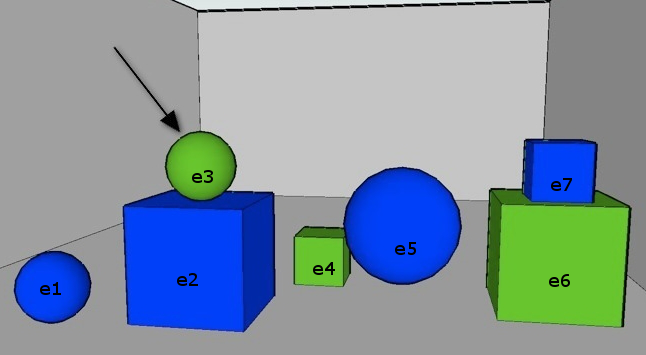
\includegraphics[width=0.5\textwidth]{images/3b.png}
\caption{Contexto de ejemplo}\label{GRE3D7-stimulus-cap2}
%\end{minipage}
\end{center}
\end{figure}

%\textcolor{blue}{hice mas grande la figura porque no se leian, como la pase a espaniol y se me fue al pie, no se porque}
%\hspace*{-0.35cm}
\begin{figure}[ht]
\begin{center}
%\begin{minipage}[b]{0.5\linewidth}
%\centering
\begin{tikzpicture}
  [
    n/.style={circle,fill,draw,inner sep=3pt,node distance=2.6cm},
    aArrow/.style={->, >=stealth, semithick, shorten <= 2pt, shorten >= 2pt},
  ]
 \node[n,label=above:$e_1$,label=below:{
    \relsize{-1}$\begin{array}{c}
      \nLeft\\[-2pt]
      \nSmall\\[-2pt] 
      \nBlue \\[-2pt] 
      \nBall\end{array}$}] (a) {};

 \node[n,label=above:$e_2$,label=below:{
    \relsize{-1}$\begin{array}{c}
      \nLeft\\[-2pt]
      \nBig\\[-2pt] 
      \nBlue\\[-2pt] 
      \nCube\end{array}$}, right of=a] (b) {};

 \node[n,label=below:$e_3$,label=above:{
    \relsize{-1}$\begin{array}{c}
      \nTop\\[-2pt]
      \nLeft\\[-2pt]
      \nSmall\\[-2pt] 
      \nGreen\\[-2pt] 
      \nBall\end{array}$}, above of=b] (c) {};

 \node[n,label=above:$e_4$,label=below:{
    \relsize{-1}$\begin{array}{c}
      \nSmall\\[-2pt] 
      \nGreen\\[-2pt] 
      \nCube\end{array}$}, right of=b] (d) {};

 \node[n,label=above:$e_5$,label=below:{
    \relsize{-1}$\begin{array}{c}
      \nBig\\[-2pt] 
      \nBlue\\[-2pt] 
      \nBall\end{array}$}, right of=d] (e) {};

 \node[n,label=above:$e_6$,label=below:{
    \relsize{-1}$\begin{array}{c}
      \nBig\\[-2pt] 
      \nGreen\\[-2pt] 
      \nCube\end{array}$}, right of=e] (f) {};

 \node[n,label=below:$e_7$,label=above:{
    \relsize{-1}$\begin{array}{c}
      \nTop\\[-2pt]
      \nSmall\\[-2pt] 
      \nBlue\\[-2pt] 
      \nCube\end{array}$}, above of=f] (g) {};

 \draw [aArrow,bend right=90] (b) to node[auto,swap]{\relsize{-1}$\nBelow$} (c);
 \draw [aArrow,bend right=90] (c) to node[auto,swap]{\relsize{-1}$\nOntop$} (b);

 \draw [aArrow,bend right=70] (d) to node[auto,swap]{\relsize{-1}$\nLeftof$} (e);
 \draw [aArrow,bend right=70] (e) to node[auto,swap]{\relsize{-1}$\nRightof$} (d);

 \draw [aArrow,bend right=90] (f) to node[auto,swap]{\relsize{-1}$\nBelow$} (g);
 \draw [aArrow,bend right=90] (g) to node[auto,swap]{\relsize{-1}$\nOntop$} (f);

 \draw[dotted] (-.6,-1.4) rectangle (12.5,4.5);

 \end{tikzpicture}
\caption{Modelo relacional del Contexto \ref{GRE3D7-stimulus-cap2}}
\label{GRE3D7-stimulus-graph}
%\end{minipage}
\end{center}
\end{figure}

Algoritmos de refinamiento para GER se basan en la siguiente idea b\'asica:
dada una escena $S$, los objetos que aparecen en $S$ son sucesivamente
clasificados de acuerdo con sus propiedades en clases m\'as y m\'as finas. 
Una descripci\'on (en alg\'un lenguaje formal de $\mathcal{L}$) de cada
clase se calcula cada vez que una clase es refinada. El procedimiento siempre
se detiene cuando el conjunto de clases se estabiliza, es decir, no se puede hacer m\'as refinamiento
con la informaci\'on disponible en la escena \footnote{Por supuesto, si s\'olo estamos interesados en una expresi\'on referencial de un objeto dado, se puede detener el procedimiento en cuanto el objetivo es el
   \'unico elemento de alguna de las clases.}

Si el elemento target est\'a en
una clase singleton, entonces la descripci\'on formal de esa clase es un
expresi\'on referencial; de lo contrario el target no puede ser un\'{i}vocamente
descripto (en $\mathcal{L}$).\\

Est\'a claro que una escena puede ser codificada en diferentes formas como un
modelo relacional (por ejemplo, en \ref{GRE3D7-stimulus-cap2}, podr\'{i}amos argumentar que
$e_1$ es tambi\'en \emph{leftof} $e_2$, pero no lo consideramos porque no se estan 
tocando en la imagen). El algoritmo asume que estas cuestiones se han resuelto y que el modelo codifica una representaci\'on adecuada de la escena que
queremos describir. Por otra parte, vamos a suponer que todas las relaciones son
\emph{binarias}. No vamos a considerar las relaciones de aridad mayor que
dos (relaciones de mayor aridad pueden codificarse como relaciones binarias v\'{i}a
reificaci\'on, si es necesario).\\

%On termination, the algorithm computes what are called the
%$\mathcal{L}$-similarity classes of the input model $\gM$.
%Intuitively, the referring expression ``\textsf{ball}'' and ``\textsf{cube}''  are more specific and then contain more information than $\top$.


Tras la resoluci\'on, el algoritmo calcula lo que se llama la
$\mathcal{L}$ - clases de semejanza del modelo de entrada de $\gM$.\\

%There is many $\mathcal{L}$, we will name $\alc$ and $\el$

%ACA VOY A PONER gramatica para generar... ALC y EL no quedaria bien aca, hay que ver lo agregamos antes o no hace falta
%In what follows, we use formulas of the $\el$ description logic
%language
En lo que sigue, se utilizan f\'ormulas de la descripci\'on de la l\'ogica $\el$
~\cite{baad:desc03} para describir las clases de refinamiendo
\footnote{N\'otese, sin embargo, que el lenguaje formal particular usado es
   independiente del algoritmo principal, y diferentes funciones
  add$_{\mathcal{L}}$($\varphi$,\RE) se pueden utilizar dependiendo
   de la l\'ogica en cuesti\'on.}. como se discuti\'o 
en~\cite{arec2:2008:Areces}, 
este lenguaje es adecuado para describir
RE conjuntivas y relacionales, que son lo que encontramos en los corpus.

  La entrada al algoritmo ser\'a un modelo $\mathcal{M} =
 \tup{\Delta, \interp{\cdot}}$, donde $\Delta$ es el dominio no vac\'io de objetos de la imagen,
 $\interp{\cdot}$ es una funci\'on de interpretaci\'on que asigna a todas las propiedades de la escena su extensi\'on.
 Por ejemplo, la escena mostrada en la Figura~\ref{GRE3D7-stimulus-cap2} podr\'ia ser representada por el modelo
 $\gM=\tup{\Delta,\interp{\cdot}}$ mostrado en la 
 Figura~\ref{GRE3D7-stimulus-graph}; donde+- $\Delta =
 \{e_1,\ldots,e_7\}$, e $\interp{\textsf{red}}$ is $\{e_2, e_4, e_5,
 e_7\}$.

Se llama extensi\'on de una f\'ormula al conjunto de objetos que la hacen v\'alida.

$\top$ es una f\'ormula que representa la descripci\'on m\'as general, cuya
interpretaci\'on incluye todos los elementos del modelo. Se podr\'ia realizar
como la ER con el sustantivo
``\textsf{cosa}''. Decimos que una f\'ormula es
\emph{subsumida} por otras f\'ormulas, cuando su extensi\'on puede ser cubierta por la
union de las extensiones de las otras f\'ormulas. Por ejemplo, en la
Figura~\ref{GRE3D7-stimulus-cap2}, $\top$ es subsumida por ``\textsf{ball}'' y
``\textsf{cube}'', porque $\interp{\top}$ = $\interp{\textsf{ball}}
\cup \interp{\textsf{cube}}$.
%= $\{e_2, e_4, e_6, e_7\}$, it is $\{e_1, e_2, e_3, e_4, e_5, e_6, e_7\}$ = $\{e_1, e_3, e_5\} \cup \{e_2, e_4, e_6, e_7\}$. 
Intuitivamente la f\'ormula ``\textsf{cube}'' o ``\textsf{ball}'' tienen m\'as informaci\'on que $\top$, para cada elemento de $\top$, hay una f\'ormula que d\'a m\'as informaci\'on, digamos ``\textsf{cube}'' es m\'as informativa que ``\textsf{cosa}''.\\

%In the following we will explain an example of execusion of the
%algorithm shown in Figure
%A continuaci\'on vamos a explicar un ejemplo de ejecusi\'on del
%algoritmo mostrado en la Figura~\ref{algoritmoOriginal} considerando la l\'ogica 
%$\el$ como language. Este algoritmo fue presentado en
%~\cite{arec2:2008:Areces}.
%
%\begin{figure}[h!]
%\begin{center}
%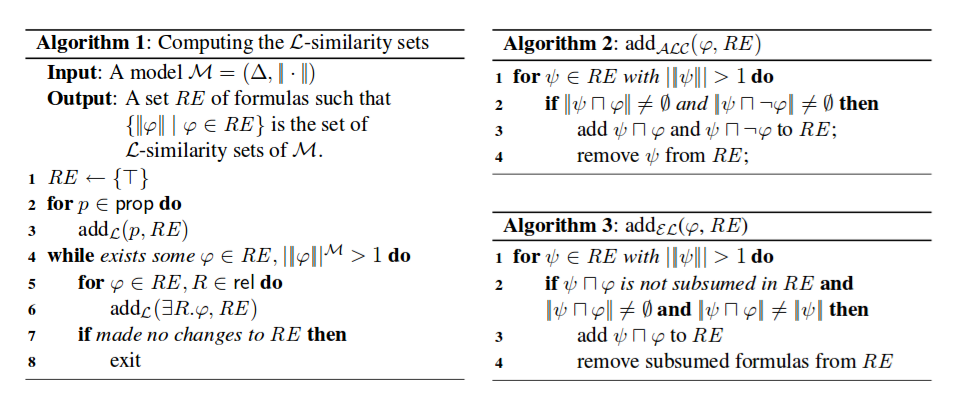
\includegraphics[width=\textwidth]{images/algoritmoOriginal.png}
%\end{center}
%\vspace*{-2em}
%\caption{Algoritmo para GER con l\'ogicas de descripci\'on}
%\label{algoritmoOriginal}
%\end{figure}

%\subsection{Ejemplo de ejecuci\'on}
%
%
%
%\textcolor{blue}{no se si poner aca un ejemplo, si poner el texto y las im\'agenes en otro apendice... o ponerlas mas chiquitas en varias columnas, asi queda feo}\\
%Vamos a ejecutar el algoritmo para la Figura~\ref{GRE3D7-stimulus-cap2},
%el algoritmo comienza con una lista fija de propiedades y relaciones, supongamos que
%esas listas son las siguientes:
%
%propiedades ordenadas (prop): \textsf{ball}, \textsf{cube}, \textsf{red}, \textsf{yellow}, \textsf{small}, \textsf{large}.\\
%relaciones ordenadas (rel): \textsf{leftof}, \textsf{rightof}, \textsf{ontopof}, \textsf{bellowof}.
%
%%\begin{figure}
%%\begin{center}	
%%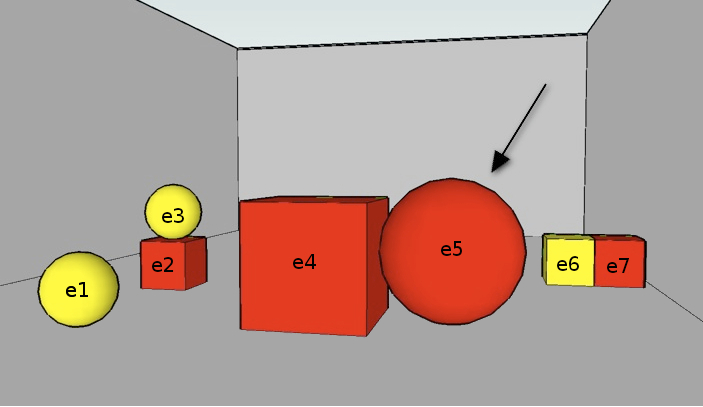
\includegraphics[width=.5\textwidth]{images/22.jpg}
%%\end{center}
%%\vspace*{-1.5em}
%%\caption{Escena 3D de figuras geom\'etricas}\label{figure22}
%%\end{figure}
%
%%\begin{figure}
%%\begin{minipage}[b]{0.6\linewidth}
%%\centering
%%\begin{tikzpicture}
%%  [
%%    n/.style={circle,fill,draw,inner sep=3pt,node distance=1.4cm},
%%    aArrow/.style={->, >=stealth, semithick, shorten <= 2pt, shorten >= 2pt},
%%  ]
%% \node[n,label=above:$e_1$,label=below:{
%%    \relsize{-1}$\begin{array}{c}
%%      \nLeft\\[-2pt]
%%      \nSmall\\[-2pt] 
%%      \nYellow \\[-2pt] 
%%      \nBall\end{array}$}] (a) {};
%
%% \node[n,label=above:$e_2$,label=below:{
%%    \relsize{-1}$\begin{array}{c}
%%      \nLeft\\[-2pt]
%%      \nSmall\\[-2pt] 
%%      \nRed\\[-2pt] 
%%      \nCube\end{array}$}, right of=a] (b) {};
%
%% \node[n,label=below:$e_3$,label=above:{
%%    \relsize{-1}$\begin{array}{c}
%%      \nTop\\[-2pt]
%%      \nLeft\\[-2pt]
%%      \nSmall\\[-2pt] 
%%      \nYellow\\[-2pt] 
%%      \nBall\end{array}$}, above of=b] (c) {};
%
%% \node[n,label=above:$e_4$,label=below:{
%%    \relsize{-1}$\begin{array}{c}
%%      \nBig\\[-2pt] 
%%      \nRed\\[-2pt] 
%%      \nCube\end{array}$}, right of=b] (d) {};
%
%% \node[n,label=above:$e_5$,label=below:{
%%    \relsize{-1}$\begin{array}{c}
%%      \nBig\\[-2pt] 
%%      \nRed\\[-2pt] 
%%      \nBall\end{array}$}, right of=d] (e) {};
%
%% \node[n,label=above:$e_6$,label=below:{
%%    \relsize{-1}$\begin{array}{c}
%%      \nSmall\\[-2pt] 
%%      \nYellow\\[-2pt] 
%%      \nCube\end{array}$}, right of=e] (f) {};
%
%% \node[n,label=above:$e_7$,label=below:{
%%    \relsize{-1}$\begin{array}{c}
%%      \nSmall\\[-2pt] 
%%      \nRed\\[-2pt] 
%%      \nCube\end{array}$}, right of=f] (g) {};
%
%% \draw [aArrow,bend right=90] (b) to node[auto,swap]{\relsize{-1}$\nBelow$} (c);
%% \draw [aArrow,bend right=90] (c) to node[auto,swap]{\relsize{-1}$\nOntop$} (b);
%
%% \draw [aArrow,bend right=30] (d) to node[auto,swap]{\relsize{-1}$\nLeftof$} (e);
%% \draw [aArrow,bend right=30] (e) to node[auto,swap]{\relsize{-1}$\nRightof$} (d);
%
%% \draw [aArrow,bend right=30] (f) to node[auto,swap]{\relsize{-1}$\nLeftof$} (g);
%% \draw [aArrow,bend right=30] (g) to node[auto,swap]{\relsize{-1}$\nRightof$} (f);
%
%% \draw[dotted] (-.4,-1.7) rectangle (7.5,3.3);
%
%% \end{tikzpicture}
%%\caption{La escena como modelo relacional}\label{GRE3D7-stimulus-graph}
%%\end{minipage}
%%\end{figure}
%
%
%El algoritmo siempre termina, y devuelve ER un conjunto de f\'ormulas que describe cada elemento en el dominio (si existe esa f\'ormula). \\
%
%En el comienzo ER=$\{\top\}$ y $\interp{\top}$ = $\{e_1, e_2, e_3, e_4, e_5, e_6, e_7\}$ como se puede ver en la Figura~\ref{fig-modelo}.\\
%
%ACA
%\begin{figure}[ht]
%\begin{minipage}[b]{0.45\linewidth}
%\centering
%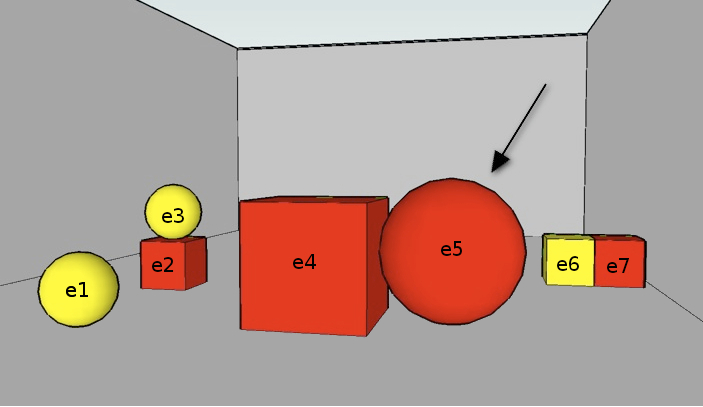
\includegraphics[width=\textwidth]{images/22.jpg}
%\vspace*{1cm}
%%\caption{Input scene}
%\label{GRE3D7-stimulus-22}
%\end{minipage}
%%\hspace*{-0.35cm}
%\begin{minipage}[b]{0.6\linewidth}
%\centering
%%\begin{figure}[ht]
%%\begin{center}
%\frame{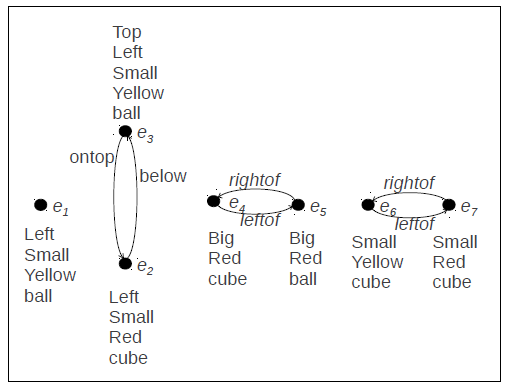
\includegraphics[width=8cm]{images/modelo.png}}\\[0pt]
%\caption{Modelo de la Figura \ref{GRE3D7-stimulus-22}}
%\label{fig-modelo}
%\end{minipage}
%\end{figure}
%El primer bucle del algoritmo es en las propiedades. Para cada propiedad hace add$_\el$ ($\varphi$, RE), las propiedades at\'omicas se muestran en la Figura~\ref{fig-modelo2}.
%
%\begin{figure}[ht]
%\begin{center}
%\frame{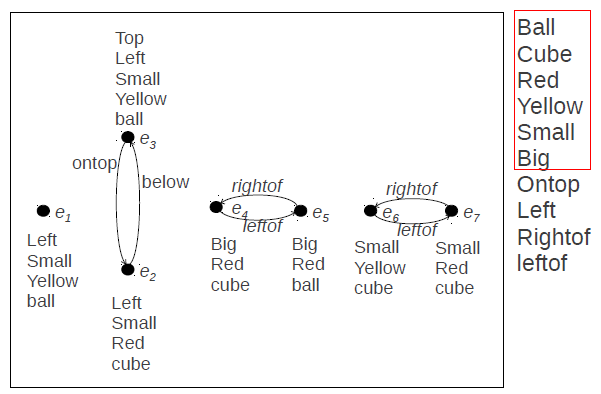
\includegraphics[width=8cm]{images/modelo2.png}}\\[0pt]
%\caption{Propiedades proposicionales en cuadro rojo, las del primer ciclo del algoritmo}
%\label{fig-modelo2}
%\end{center}
%\end{figure}
%
%La f\'ormula $\varphi$ se a\~nadir\'a a ER si su interpretaci\'on tiene al menos un elemento, a continuaci\'on, para cada f\'ormula
 %$\psi$ en ER la conjunci\'on
%$\varphi  \wedge \psi$ no necesita estar subsumida in ER, la $\interp{\varphi \cup \psi}$ no tiene que ser vac\'io, y su interpretaci\'on tiene que ser distinta de $\interp{\psi}$. Luego las f\'ormulas subsumidas se borran.
%
%La primer propiedad es \textsf{ball}, ER = \{$\top$, \textsf{ball}\}, se ven los elementos de ``ball'' en un recuadro en la Figura~\ref{fig-modelo3}.
%
%\begin{figure}[ht]
%\begin{center}
%\frame{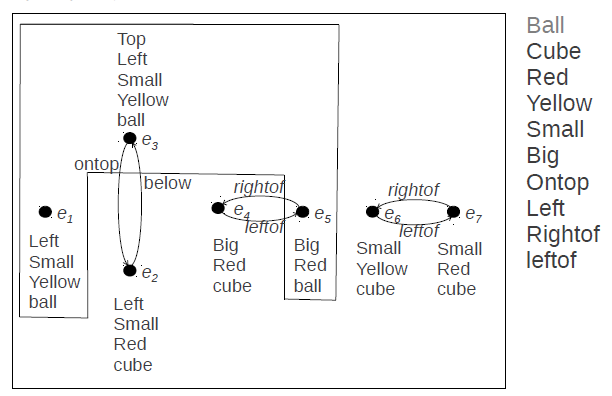
\includegraphics[width=8cm]{images/modelo3.png}}\\[0pt]
%\caption{El cuadro indica cuales son ``ball''}
%\label{fig-modelo3}
%\end{center}
%\end{figure}
%
%La siguiente propiedad es \textsf{cube}, ER = \{$\top$, \textsf{ball}, \textsf{cube}\}, pero ahora la $\interp{\textsf{ball}}$ = $\{e_1, e_3, e_5\}$, $\interp{\textsf{cube}}$ = $\{e_2, e_4, e_6, e_7\}$, quedando las particiones como se muestra en la Figura~\ref{fig-modelo4}
%\begin{figure}[ht]
%\begin{center}
%\frame{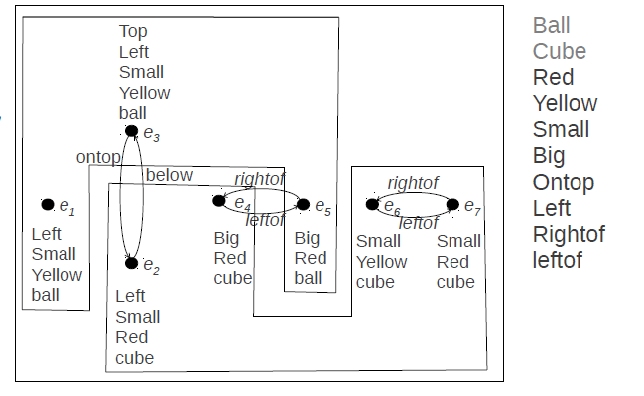
\includegraphics[width=8cm]{images/modelo4.png}}\\[0pt]
%\caption{Cuadros indicando ``ball'' y ``cube''}
%\label{fig-modelo4}
%\end{center}
%\end{figure}
%Ahora podemos borrar $\top$, porque es subsumida (esta cubierta por) las otras dos f\'ormulas. La siguiente propiedad es  \textsf{red}, $\interp{\textsf{red}}$ es: $\{e_2, e_4, e_5, e_7\}$, haciendo la intersecci\'on con la $\interp{.}$ de cada f\'ormula en ER obtenemos, $\{e_5\}$ y $\{e_2, e_4, e_7\}$, ER = $\{\textsf{ball}, \textsf{cube}, \textsf{ball} \wedge \textsf{red}, \textsf{cube} \wedge \textsf{red}\}$, las particiones actuales se pueden ver en la Figura~\ref{fig-modelo9}.
%\begin{figure}[ht]
%\begin{center}
%\frame{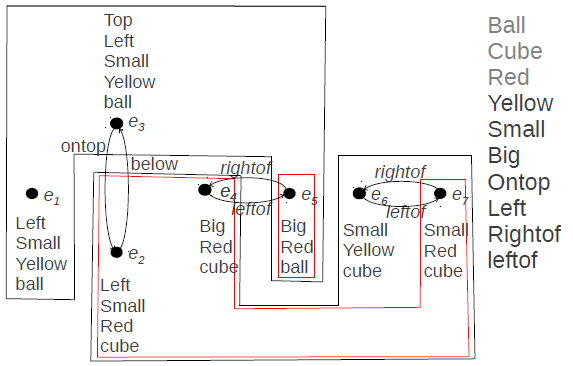
\includegraphics[width=8cm]{images/modelo9.png}}\\[0pt]
%\caption{Cuadros indicando ``ball'', ``cube'' y ``red''}
%\label{fig-modelo9}
%\end{center}
%\end{figure}
%
%Siguiendo con \textsf{yellow}, tenemos, $\interp{\textsf{yellow}}$ = $\{e_1, e_3, e_6\}$ y obtenemos ER = $\{\textsf{ball} \wedge \textsf{yellow}, \textsf{cube} \wedge \textsf{yellow}, \textsf{ball} \wedge \textsf{red}, \textsf{cube} \wedge \textsf{red}\}$. 
%Note que aqu\'i ya borramos la f\'ormula \textsf{ball} porque estaba subsumida, y la f\'ormula \textsf{cube} tambi\'en. Se muestran particiones en Figura~\ref{fig-modelo10}.
%
%\begin{figure}[ht]
%\begin{center}
%\frame{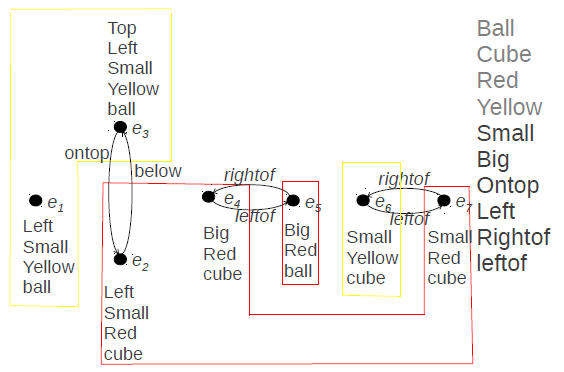
\includegraphics[width=8cm]{images/modelo10.png}}\\[0pt]
%\caption{Cuadros indicando ``ball'', ``cube'', ``red'' y ``yellow''}
%\label{fig-modelo10}
%\end{center}
%\end{figure}
%
%Haciendo lo mismo con \textsf{small} tenemos ER = $\{\textsf{ball} \wedge \textsf{yellow} \wedge \textsf{small}, \textsf{cube} \wedge \textsf{yellow} \wedge \textsf{small}, \textsf{ball} \wedge \textsf{red}, \textsf{cube} \wedge \textsf{red}, \textsf{cube} \wedge \textsf{red} \wedge \textsf{small}\}$, como se puede ver en Figura~\ref{fig-modelo11}.
%\begin{figure}[ht]
%\begin{center}
%\frame{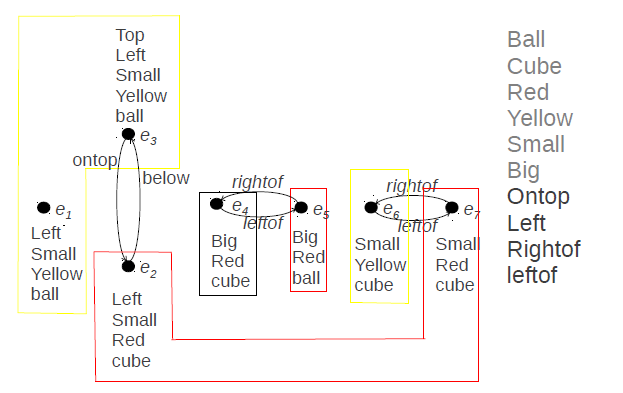
\includegraphics[width=8cm]{images/modelo11.png}}\\[0pt]
%\caption{Cuadros indicando ``ball'', ``cube'', ``red'', ``yellow'', ``small'' y ``large''}
%\label{fig-modelo11}
%\end{center}
%\end{figure}
%
%La siguiente propiedad es \textsf{large} as\'i, tenemos ER = $\{\textsf{ball} \wedge \textsf{yellow} \wedge \textsf{small}, \textsf{cube} \wedge \textsf{yellow} \wedge \textsf{small}, \textsf{ball} \wedge \textsf{red}, \textsf{cube} \wedge \textsf{red} \wedge \textsf{large}, \textsf{cube} \wedge \textsf{red} \wedge \textsf{small}\}$. Aqu\'i no podemos agregar \textsf{large} a la f\'ormula $\textsf{red} \wedge \textsf{cube}$ porque su interpretaci\'on tiene un solo elemento, y la condici\'on dice que es necesario tener m\'as de uno.
%
%Hasta ahora ER = $\{\textsf{ball} \wedge \textsf{yellow} \wedge \textsf{small}, \textsf{cube} \wedge \textsf{yellow} \wedge \textsf{small}, \textsf{ball} \wedge \textsf{red}, \textsf{cube} \wedge \textsf{red} \wedge \textsf{large}, \textsf{cube} \wedge \textsf{red} \wedge \textsf{small}\}$ 
%y tenemos las siguientes extensiones: $\{e_1, e_3\}, \{e_6\}, \{e_5\}, \{e_4\}, \{e_2, e_7\}$ respectivamente. 
%Hay dos f\'ormulas que a\'un pueden ser refinadas, $\textsf{ball} \wedge \textsf{yellow} \wedge \textsf{small}$ y $\textsf{cube} \wedge \textsf{red} \wedge \textsf{small}$ 
%debido a que tienen m\'as de un elemento cada una, por lo que entran en el ciclo, while del algoritmo 1, en la l\'inea 4. Ahora es el turno de las relaciones, la primera de ellas es \textsf{leftof}, para cada f\'ormula $\varphi$ en ER trataremos de hacer add$_\el$ ($\exists \textsf{leftof}.\varphi$, RE). Notar que $\psi$ solo puede ser $\textsf{ball} \wedge \textsf{yellow} \wedge \textsf{small}$ o $\textsf{cube} \wedge \textsf{red} \wedge \textsf{small}$ porque esos son los que su interpretaci\'on tiene m\'as de un elemento. 
%\begin{figure}[ht]
%\begin{center}
%\frame{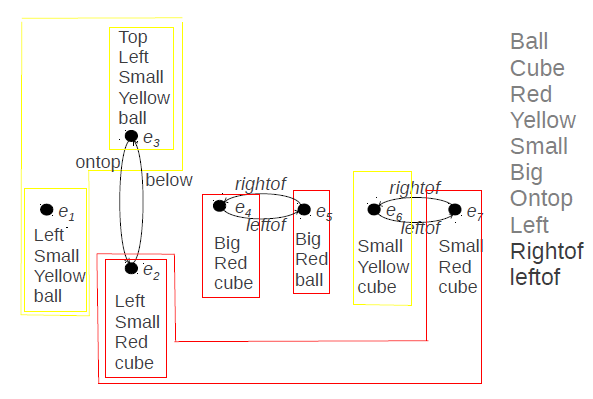
\includegraphics[width=8cm]{images/modelo15.png}}\\[0pt]
%\caption{Cuadros indicando ``ball'', ``cube'', ``red'', ``yellow''...}
%\label{fig-modelo15}
%\end{center}
%\end{figure}
%
%
%No hay
%%because those are the ones that its interpretation have more than one element. There is not 
%$\varphi$ y $\psi$ que puedan ser aplicadas. Continuando con \textsf{rightof} agregamos $\textsf{cube} \wedge \textsf{yellow} \wedge \textsf{small} \wedge \exists \textsf{rightof}. \textsf{cube} \wedge \textsf{red} \wedge \textsf{small}$, y asi con \textsf{topof} agregamos $\textsf{small} \wedge \textsf{red} \wedge \textsf{cube} \wedge \exists \textsf{ontop}. \textsf{small} \wedge \textsf{yellow} \wedge \textsf{ball}$ y el algoritmo termina con ER = $\{\textsf{ball} \wedge \textsf{yellow} \wedge \textsf{small}, \textsf{cube} \wedge \textsf{yellow} \wedge \textsf{small}, \textsf{ball} \wedge \textsf{red}, \textsf{cube} \wedge \textsf{red} \wedge \textsf{large}, \textsf{cube} \wedge \textsf{red} \wedge \textsf{small}, \textsf{cube} \wedge \textsf{yellow} \wedge \textsf{small} \wedge \exists \textsf{rightof}. \textsf{cube} \wedge \textsf{red} \wedge \textsf{small}, \textsf{small} \wedge \textsf{red} \wedge \textsf{cube} \wedge \exists \textsf{ontop}. \textsf{small} \wedge \textsf{yellow} \wedge \textsf{ball}\}$, 
%aqu\'i todos los elementos est\'an en una clase singleton y no se puede hacer ning\'un refinamiento m\'as. 
%%can be applied to $cube \wedge red \wedge small$ but there is no formula which interpretation has more than one element to be apply with this one. The same happen for the other relations, so the algorithm ends.
%%its interpretation is $\{e_7\}$ with $\psi$ is $cube \wedge yellow \wedge small$, the others combinations can't be apply because they don't do true the preconditions. The following relation is rightof, 
%
%%leftof, rightof, ontopof, bellowof
%
%%At this point we already have the target in a singleton set. So the formula for it is ``red and ball'', and also for s6 which formula is ``yellow cube''.\\
%%As we show this algorithm depends of the order of properties and relations.\\
%\begin{figure}[ht]
%\begin{center}
%\frame{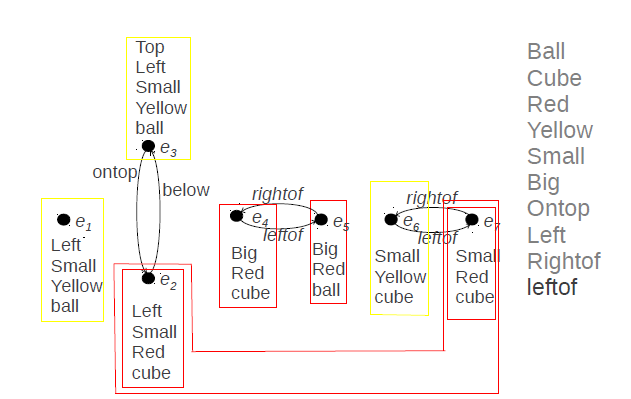
\includegraphics[width=8cm]{images/modelo16.png}}\\[0pt]
%\caption{Cuadros indicando ``ball'', ``cube'', ``red'', ``yellow''...}
%\label{fig-modelo16}
%\end{center}
%\end{figure}
%
%\begin{figure}[ht]
%\begin{center}
%\frame{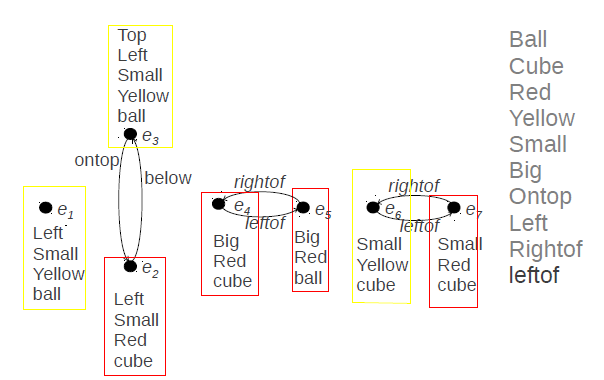
\includegraphics[width=8cm]{images/modelo17.png}}\\[0pt]
%\caption{Cuadros indicando ``ball'', ``cube'', ``red'', ``yellow''...}
%\label{fig-modelo17}
%\end{center}
%\end{figure}
%
%Las expresiones referenciales encontradas son:\\
%
%$\textsf{ball} \wedge \textsf{yellow} \wedge \textsf{small}$ representa $e_1$ \\
%$\textsf{cube} \wedge \textsf{yellow} \wedge \textsf{small}$ representa $e_6$ \\
%$\textsf{ball} \wedge \textsf{red}$ representa $e_5$ \\
%$\textsf{cube} \wedge \textsf{red} \wedge \textsf{large}$ representa $e_4$ \\
%$\textsf{cube} \wedge \textsf{red} \wedge \textsf{small}$ representa $\{e_2,e_7\}$  \\
%$\textsf{cube} \wedge \textsf{yellow} \wedge \textsf{small} \wedge \exists \textsf{rightof}. \textsf{cube} \wedge \textsf{red} \wedge \textsf{small}$ representa $e_6$ \\
%$\textsf{small} \wedge \textsf{red} \wedge \textsf{cube} \wedge \exists \textsf{ontop}. \textsf{small} \wedge \textsf{yellow} \wedge \textsf{ball}$ representa $e_2$ \\
%



\section{Aproximaciones emp\'iricas a la soluci\'on de GER}

\subsection{Corpus existente}
\label{sec:corpus2}
\label{sec:corpusTUNA}

%was the first prominent REG corpus to be made publicly available for research purposes. The corpus was developed in a series of general-purpose controlled experiments, containing 2280 descriptions produced by 60 speakers in two domains (1200 descriptions of furniture items and 1080 descriptions of people's photographs). TUNA does not contain relational descriptions, and it is possibly the only resource of this kind to include situations of reference to sets. The TUNA corpus has been extensively used in a series of shared tasks

TUNA \cite{tuna-corpus} fue el primer corpus prominente para GER disponible p\'ublicamente con fines de investigaci\'on. El corpus fue desarrollado en una serie de experimentos controlados de prop\'osito general, contiene 2.280 descripciones producidas por 60 personas en dos dominios (1.200 expresiones referenciales de im\'agenes de muebles y 1080 expresiones referenciales de fotograf\'ias de personas situadas en una grilla). Se muestran ejemplos de im\'agenes en Figuras \ref{fig-TUNA-furniture} y \ref{fig-TUNA-people}. El corpus TUNA no contiene descripciones relacionales, y es posiblemente el \'unico recurso de este tipo que incluye situaciones de referencia a conjuntos. Este corpus se ha utilizado ampliamente en una serie de desaf\'ios \cite{reg2009}. \\

\begin{figure}
\begin{minipage}[t]{0.5\linewidth}
\centering
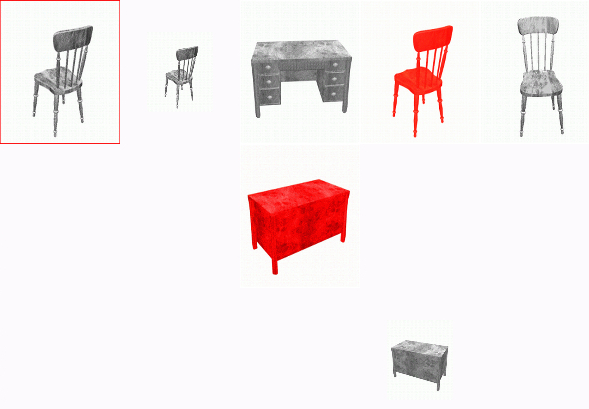
\includegraphics[width=\textwidth]{images/largeGreyChair.jpg}\\[0pt]
\caption{Imagen del TUNA corpus (muebles)}
\label{fig-TUNA-furniture}
\vspace*{.1cm}
\end{minipage}
\hspace*{0cm}
\begin{minipage}[t]{0.5\linewidth}
\centering
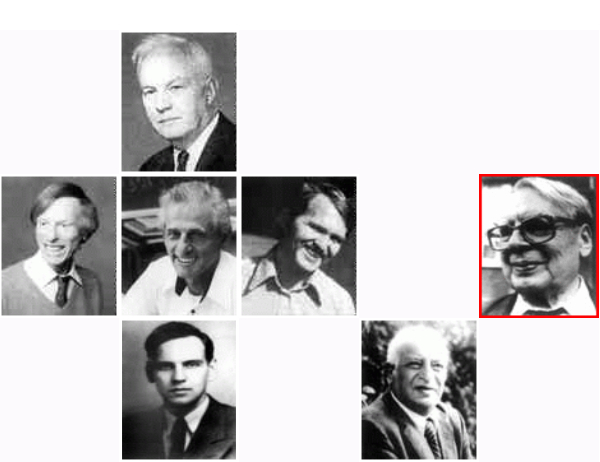
\includegraphics[width=\textwidth]{images/tuna-people.jpg}\\[0pt]
\caption{Imagen del TUNA corpus (personas)}
\label{fig-TUNA-people}
\end{minipage}
\end{figure}


\label{sec:corpusGRE}
%were developed in a series of web-based experiments primarily focussed on the study of relational descriptions. GRE3D3 contains 630 descriptions produced by 63 speakers, and GRE3D7 contains 4480 descriptions produced by 287 speakers, making it the largest of its kind to date. The GRE3D domain consists of simple visual scenes containing only two kinds of objects (boxes and spheres) with limited variation in colour and size. In each scene, there is only one possible spatial relation between target and the nearest landmark. Both corpora contain atomic and relational descriptions.
GRE3D3 y su extensi\'on GRE3D7 \cite{gre3d3,gre3d7} se desarrollaron en una serie de experimentos basados en la web, se centraron principalmente en el estudio de las descripciones relacionales. GRE3D3 contiene 630 descripciones producidas por 63 personas y GRE3D7 contiene 4.480 descripciones producidas por 287 personas, y es el corpus m\'as grande de este tipo hasta la fecha. El dominio del GRE3D3 consta de escenas visuales simples que contienen s\'olo dos tipos de objetos (cubos y esferas) con variaci\'on limitada en color y tama\~no. En cada escena, s\'olo hay una posible relaci\'on espacial entre el target y el landmark m\'as cercano. Ambos corpus contienen descripciones at\'omicas y relacionales. Ejemplo de im\'agenes del GRE3D3 y GRE3D7 se muestran en las Figuras \ref{fig-GRE3D3} y \ref{fig-GRE3D7}.\\
%\begin{minipage}[b]{0.45\linewidth}

\begin{figure}
\begin{minipage}[b]{0.5\linewidth}
\centering
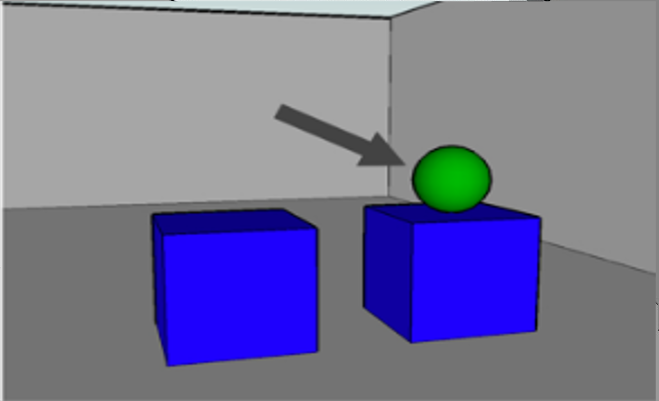
\includegraphics[width=\textwidth]{images/GRE3D3.png}\\[0pt]
\caption{Imagen del GRE3D3}
\label{fig-GRE3D3}
\vspace*{-0.7cm}
\end{minipage}
\hspace*{0cm}
\begin{minipage}[b]{0.5\linewidth}
\centering
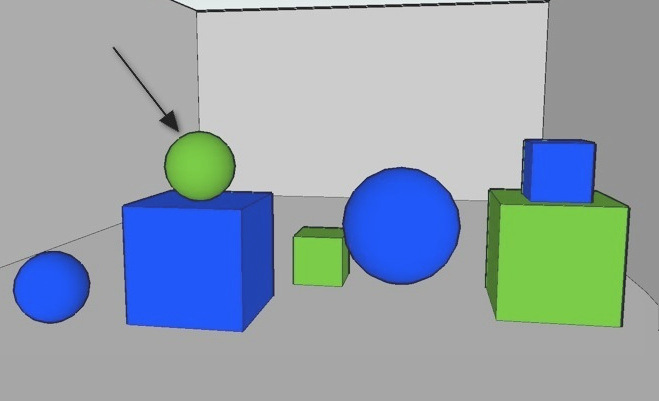
\includegraphics[width=\textwidth]{images/3.jpg}\\[0pt]
\caption{Imagen del GRE3D7}
\label{fig-GRE3D7}
\end{minipage}
\end{figure}

%\vspace*{3cm}

\label{sec:corpusSTARS}
%and its extension Stars2 were collected for the study of referential overspecification (particularly in the case of relational descriptions). Stars was developed in a pilot web-based experiment, containing 704 descriptions produced by 64 speakers.  The more comprehensive Stars2 data set was produced in dialogue situations involving subject pairs, and it contains 884 descriptions produced by 56 speakers. Both domains make use of simple visual scenes containing up to four object types (e.g., stars, boxes, cones and spheres) with limited variation in colour and size. Differently from other REG corpora, however, Stars/2 includes a considerable number of complex situations of reference involving up to three objects, as in `the box near the sphere, next to the cone'.http://ppgsi.each.usp.br/arquivos/RelTec/PPgSI-002_2014.pdf y http://ppgsi.each.usp.br/arquivos/RelTec/PPgSI-001_2015.pdf
Stars \cite{stars-mutual-disamb} y su extensi\'on Stars2 se colectaron para el estudio de la sobre-especificaci\'on (particularmente en el caso de las descripciones relacionales). Stars se desarroll\'o en un experimento piloto basado en la web, contiene 704 descripciones producidas por 64 personas. El conjunto de datos Stars2 es m\'as completo y se obtuvo de situaciones de di\'alogo que implicaban a dos personas, contiene 884 descripciones producidas por 56 participantes. Ambos dominios hacen uso de escenas visuales simples que contienen tres tipos de objetos (por ejemplo para Stars, estrellas, cuadrados y c\'irculos y para Stars2 cubos, conos y esferas) con variaci\'on limitada en color y tama\~no. A diferencia de otros corpus para GER, Stars/2 incluyen un n\'umero considerable de situaciones complejas de referencia en que participan hasta tres objetos, como en ``el cubo cerca de la esfera, al lado del cono''. Ejemplos de imagenes se muestran en las Figuras \ref{fig-STARS} y \ref{fig-STARS2}.\\


\begin{figure}
\begin{minipage}[b]{0.5\linewidth}
\centering
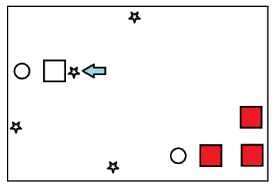
\includegraphics[width=\textwidth]{images/STARS.png}\\[0pt]
\caption{Imagen de Stars corpus}
\label{fig-STARS}
%\vspace*{1cm}
\end{minipage}
\hspace*{0cm}
\begin{minipage}[b]{0.5\linewidth}
\centering
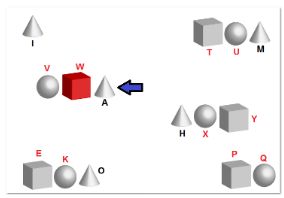
\includegraphics[width=\textwidth]{images/STARS2.png}\\[0pt]
\caption{Imagen de Stars2 corpus}
\label{fig-STARS2}
\end{minipage}
\end{figure}

%ejemplo minipage
%\begin{figure}
%\begin{minipage}[b]{0.5\linewidth}
%\centering
%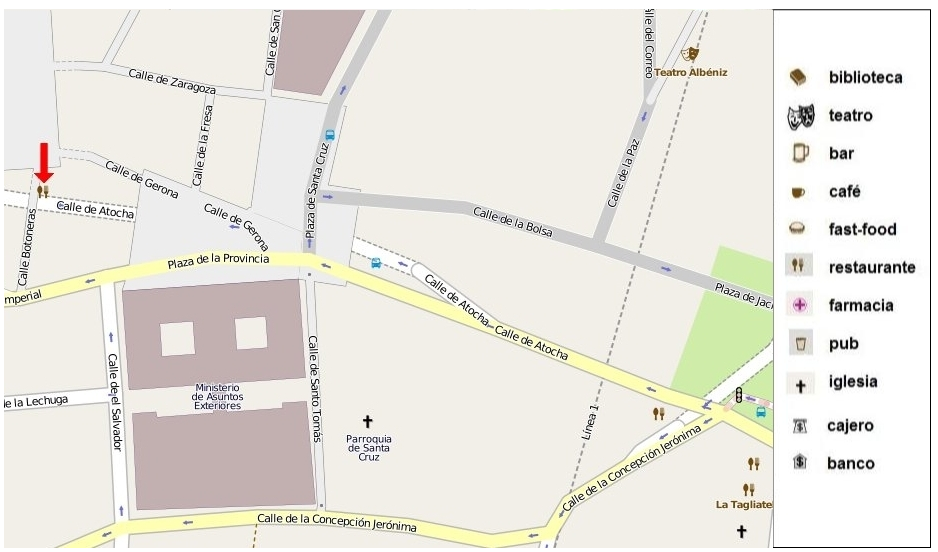
\includegraphics[width=\textwidth]{figures/rest-singular2x.png}\\[0pt]
%\caption{Target singular con zoom 2X}
%\label{rest-singular2x}
%\end{minipage}
%\vspace*{.1cm}
%\begin{minipage}[b]{0.5\linewidth}
%\centering
%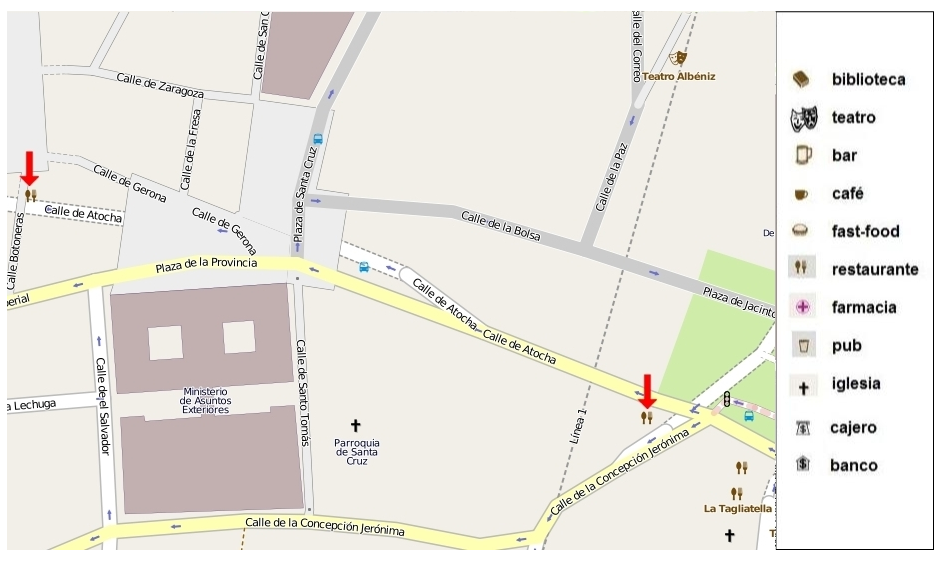
\includegraphics[width=\textwidth]{figures/rest-plural2x.png}\\[0pt]
%\caption{Target plural con zoom 2X}
%\label{rest-plural2x}
%\end{minipage}
%\end{figure}




%Despite their usefulness and general contribution to the research in REG, the above domains are still at a certain distance from the kinds of visual scene that might be required for a practical, real-world application. The need for additional complexity and/or realism, and our own interest in the surface realisation task for the Spanish and Portuguese languages, has led us to build a new computational resource of this kind. This work is described in the next sections. Further discussion on the differences between the Zoom corpus and existing resources is presented in Sec. \ref{sec-annotation}. 



\subsection{Trabajos emp\'iricos en el \'area}

%http://link.springer.com/chapter/10.1007/978-3-642-15573-4_9
%http://www.jetteviethen.net/papers/DaleViethen2010chapter.pdf

La investigaci\'on presentada en \cite{viethen-phd} se basa en dos premisas fundamentales: que la investigaci\'on
en la generaci\'on autom\'atica de expresiones referenciales debe esforzarse por lograr
sistemas que den salidas tan similar a la humana como sea posible; y que, para ello, debemos
esforzarnos para modelar el comportamiento humano como se puede observar en corpora.

La adopci\'on de estas premisas sirve para dos fines: en primer lugar, mejora la adecuaci\'on
de la salida de algoritmos de GER para el objeto target imitando la capacidad humana
de producir referencias adecuadas; y en segundo lugar, el estudio de corpus de datos producidos por humanos
 y algoritmos en desarrollo que pueden replicar estos datos podr\'ian
acercarnos a la comprensi\'on de que es lo que hacen los humanos cuando dan una ER.\\

Se\~nala que el cl\'asico algoritmo de GER y la mayor parte de sus descendientes no se basaron ni evaluaron contra datos producidos por humanos. Ellos se basaron en una visi\'on bastante minimalista de lo que se necesita
para que una expresi\'on referencial sea \'optima, concentr\'andose en la eficiencia computacional 
 y descripciones breves como sus principales preocupaciones.\\

 Existe un peque\~no n\'umero de enfoques que 
 se basaron en observaciones del comportamiento de referencia general humana
que obtuvieron a partir de experimentos psicoling\"u\'isticos, pero de nuevo no fueron evaluados
contra datos humanos.\\

Los algoritmos que se presentaron a los desaf\'ios de evaluaci\'on \cite{gatt-balz-kow:2008:ENLG} y \cite{reg2009}
fueron probados en el TUNA-Corpus, y algunos de ellos
tambi\'en tuvieron en cuenta los patrones que se encontraban en el conjunto del desarrollo. Pero hay una serie de preocupaciones en torno a la pregunta de si el TUNA-Corpus, y la forma de salida de los sistemas que se compar\'o 
en los desaf\'ios eran ideales para una evaluaci\'on de la adecuaci\'on descriptiva de GER.\\
%saque esto porque no se entiende
%A partir de los desaf\'ios que se describen en m\'as detalle y para evaluarlos en una serie de datos m\'as grande
%que contiene m\'as de una expresi\'on referencial para cada elemento est\'imulo.
Aborda tres \'areas principales en las que los corpus se puede utilizar para
promover el objetivo de la semejanza humana en la investigaci\'on sobre generaci\'on de expresiones referenciales:
evaluaci\'on, la recolecci\'on de corpus y an\'alisis y modelizaci\'on estad\'istica de
datos de corpus.\\
Comenz\'o con el an\'alisis del estado del arte de la investigaci\'on en
la generaci\'on de descripciones distintivas, trabaj\'o con relaciones espaciales y en el trabajo us\'o datos de corpus. Examin\'o una serie de opciones metodol\'ogicas que tienen que hacerse cuando se trabaja con los corpus de GER. Aqu\'i, explor\'o diferentes opciones para los desaf\'ios de recopilaci\'on de corpus, que se centran en torno al equilibrio que se necesita
entre el control de los par\'ametros experimentales tanto como sea necesario
y mantener la configuraci\'on de lo m\'as natural posible. Discuti\'o una serie de conceptos
que son de importancia para el an\'alisis de corpora de GER, tales como la naturalidad de diferentes
propiedades de los objetos, y las nociones de minimalidad y cuestiones de sobre-especificaci\'on de expresiones referenciales. Por \'ultimo, analiz\'o diferentes maneras en que la salida de un sistema se puede
comparar con los datos de corpora, bajo la premisa de que el objetivo de la comparaci\'on es
para evaluar si el sistema podr\'ia tener un modelo adecuado del comportamiento humano para la generaci\'on de expresiones referenciales.
Realiz\'o una investigaci\'on en las tres \'areas donde se puede emplear corpora en GER: Evaluaci\'on de semejanza humana, recopilaci\'on y an\'alisis de corpus, y modelado de datos de corpus. Realiz\'o un experimento de evaluaci\'on con tres de los algoritmos cl\'asicos, (1989) Algoritmo Greedy de Dale (Greedy), Dale y Haddock (1991b), Algoritmo Relacional (ra) Y Dale y Reiter (1995) Algoritmo Incremental (IA), Se pusieron a prueba en cuanto a su capacidad de
replicar las expresiones referenciales se encuentran en un grupo relativamente peque\~no de corpus de expresiones referenciales
en un dominio visual de im\'agenes puestas en una grilla.
%de rejilla de cajones de armarios ling. 
En el an\'alisis de este experimento tuvo dos resultados principales: (1) que identic\'o en particular tres 
fen\'omenos que todav\'ia plantean importantes retos para los algoritmos GER con el objetivo de replicar
el comportamiento humano, y (2) que proporciona una plataforma para la discusi\'on de una serie de
dificultades que se presentan para la evaluaci\'on basada en corpus de GER. Esto result\'o en una serie
de criterios para el dise\~no de los dos corpus que el trabajo en el resto de la tesis.
Los tres fen\'omenos en las expresiones referenciales producidas por humanos que los
algoritmos probados no fueron capaces de replicar satisfactoriamente sobre-especificaci\'on,
relaciones espaciales, y comportamiento de voluntarios espec\'ificos. Ambos
Greddy y la IA fueron capaces de generar algo de la redundancia que se encontr\'o en el corpus.
 Ni Greedy ni el IA estaban dise\~nados para ser capaz de generar expresiones referenciales que contengan relaciones entre entidades, pero el ra fue dise\~nado para incluirlas. Sorprendentemente, el
ra no s\'olo fallo en generar cualquiera de las descripciones contenidas en el corpus de evaluaci\'on; sino tambi\'en que las descripciones que se gener\'o parec\'ian m\'as como enigmas cuyo objetivo era confundir a un oyente, m\'as que ayudar en
los intentos de se\~nalar el objetivo referente. 

Una valoraci\'on te\'orica de otras aproximaciones dise\~nados para manejar las relaciones estableci\'o que ninguno de ellos incluir\'ia una relaci\'on, si no es absolutamente necesaria para distinguir el target.
La tercera observaci\'on que el experimento dejo a la vista fue que la gente no siempre hace lo mismo en la misma situaci\'on. De hecho, incluso la misma persona podr\'ia describir el mismo target de diferente manera en distintas
circunstancias. 

 None of the algorithms tested were intended to take such inter- and
intra-speaker variation into account, and only very recently have implementations
of the
ia
begun to model speaker-preferences to some degree.

No se pretend\'ia que ninguno de los algoritmos de la prueba tomara en cuenta las variaciones entre-hablantes, ni del mismo hablante. Hay implementaciones del IA que han comenzado a agregar modelo de preferencias de hablante en alg\'un grado.

Los temas generales con evaluaci\'on basada en corpus que esta experiencia de evaluaci\'on dej\'o
al descubierto fueron (1) la interdependencia estrecha entre algoritmos y la
representaci\'on subyacente de conocimiento que utilizan, (2) el no-determinismo de la generaci\'on del lenguaje natural, (3) la cuesti\'on de c\'omo comparar la salida algoritmos con gold-standar, y (4) el dominio espec\'ifico de los algoritmos de GER.\\
La discusi\'on de estos temas ha dado lugar a la siguiente lista de Evaluaci\'on en GER basado en corpus:

1. Si el corpora est\'a destinado para ser reutilizado para la evaluaci\'on comparativa de diferentes
algoritmos, una representaci\'on subyacente del dominio debe ser proporcionada para ser usada por todos los algoritmos.

2. Si queremos confiar en los resultados, el corpus debe contener tantos casos como sea posible de tantos direntes hablantes como sea posible para cada escenario referencial. 
Esto es cierto si un algoritmo es evaluado en t\'erminos de ser capaz de generar una expresi\'on referencial que suene natural, o si est\'a probado por su probabilidad de pertenecer a un modelo espec\'ifico de conducta humana de referencia, mediante la comprobaci\'on de si se puede generar todas las descripciones en un corpus.

3. Si la probabilidad de un algoritmo de ser un modelo de la conducta humana de referencia
se eval\'ua, deben utilizarse m\'etricas basadas en recuento (RECALL) y precisi\'on (PRESITION). En este
caso, el conjunto completo de las descripciones que el algoritmo proporciona para cada
escenario de referencia en virtud de cualquier ajuste de par\'ametro debe ser comparado con el
conjunto de las descripciones contenidas en el corpus para el mismo escenario referencial.
Si la capacidad m\'as orientada a la aplicaci\'on para generar una referencia es similar a la humana
se ha de evaluar, s\'olo una descripci\'on por escenario.
Esto debe hacerse utilizando m\'etricas basadas en la precisi\'on para probar c\'omo muchos de las
descripciones dadas por los algoritmos est\'an contenidas en el corpus.
4. Algoritmos que son juzgados en un dominio espec\'ifico c, no se debe asumir como
f\'acilmente adaptable a otros dominios. Idealmente, los corpus que abarcan muchos diferentes
deben estar disponibles para las pruebas de los algoritmos que generalizan en distintos tipos de dominios.
Realiz\'o 2 corpus el GRE3D3 y el GRE3D7 descriptos en \ref{sec:corpus2}

Trabaj\'o con \'arboles de decisi\'on ...
\textcolor{blue}{Aca agregar otras personas que usaron corpus para generacion de ER, Ivandre... }

%http://www.lrec-conf.org/proceedings/lrec2012/pdf/152_Paper.pdf
En el trabajo \ref{ivandre-work-corpus} presentan 2 alternativas para aprender la seleccio\'on de atributos de una expresi\'on referencial a partir de corpus. Toma los caracter\'isticas de aprendizaje como el conjunto de valores enteros que representan el poder discriminativo de cada atributo (es decir, el n\'umero de distractores que cada atributo elimina por cada atributo que tiene el target, ejemplos son color, tama\~no, etc.) 
 %For instance, in a context set as
%seen in previous Example 1, assuming that we would like to
%refer to E4, the corresponding discriminatory power values
%would be defined as d type =1, d size =1 and d colour =3.
%In the first learning method, we will attempt to learn possible
%Pj orderings (defined as nominal values) that, if applied
%to  the  Incremental  algorithm,  would  produce  the  desired
%output L for each given input C. In the second method, we
%will  use  the  input  C  to  (binary)  decide  whether  to  select
%each attribute individually.  We will call these our
%Global and Individual AS  classifiers,  which  are  discussed  sepa-
%rately below

\subsection{M\'etricas de evaluaci\'on/comparaci\'on con corpus}

Para medir la performance de los algoritmos podemos usar m\'etricas autom\'aticas o m\'etricas manuales, las m\'etricas autom\'aticas son aquellas que se calculan mediante un algoritmo y las manuales en las cuales les requerimos a personas que evaluen las expresiones referenciales.


\subsubsection{M\'etricas autom\'aticas}


La exactitud (Accuracy) se define como el porcentaje de coincidencias exactas entre cada RE producida por un ser humano y la producida por el sistema para la misma escena y target. Se considera que es una m\'etrica demasiado estricta.\\


El coheficiente Dice es una m\'etrica de comparaci\'on de conjuntos, el valor va entre 0 y 1, 1 indica un perfecto match entre los conjuntos. Para dos conjuntos A y B, Dice se calcula como sigue:\\

$Dice(A,B) = \frac{2\times|A \cap B|}{|A|+|B|}$\\

\textsc{masi} de \cite{Passonneau06measuringagreement}~es una adaptaci\'on de el coheficiente Jaccard el cual varia en favor de la similaridad cuando un conjunto es un subconjunto de otro, como Dice varia entre 0 y 1, 1 indica match perfecto. Se calcula como sigue:\\
%which biases it in favor of similarity where one set
%is a subset of the other. Like Dice, it ranges between
%0 and 1, where 1 indicates a perfect match. It is computed as follows:\\

$\textsc{masi}(A,B) = \delta \times \frac{|A \cap B|}{|A \cup B|}$ \\


donde $\delta$ es un coheficiente definido como sigue:\\


 \begin{equation}
     \delta  = \left\{
	       \begin{array}{ll}
		 0      & if A \cap B = \emptyset \\
		 1 & if A = B  \\
		 \frac{2}{3}     & if A \subset B ~or~ B \subset A\\
		 \frac{1}{3}     & otherwise
	       \end{array}
	     \right.
 \end{equation}

Intuitivamente significa que se prefieren aquellas descripciones producidas por el sistema las cuales no incluyen atributos que los humanos no incluyeron.
%Intuitively, this
%means that those system-produced descriptions are
%preferred which do not include attributes that are
%omitted by a human.  

\subsubsection{M\'etricas manuales}
\textcolor{blue}{aca me falta escribir, aunque no se si no poner todo esto en parte evaluacion}


\chapter{Decisiones metodol\'ogicas de corpus y evaluaci\'on}
\label{sec:metodologia}
\chapter{Definiendo optimalidad de una ER}
\label{sec:metodologia}

%The concept of reference is difficult to pin down exactly (Searle 1969; Abbott 2010).
%Searle therefore suggests that the proper approach is ``to examine those cases which con-
%stitute the center of variation of the concept of referring and then examine the borderline
%cases in light of similarities and differences from the paradigms'' (Searle 1969, pages
%26-27). The ``paradigms'' of reference in Reiter and Dale (2000) are
%definite descriptions
%whose primary purpose it is to
%identify their referent
%. The vast majority of recent REG
%research subscribes to this view as well. Accordingly these paradigmatic cases will also
%be the main focus of this survey, although we shall often have occasion to discuss other
%types of expressions. However, to do full justice to indefinite or attributive descriptions,
%proper names, and personal pronouns would, in our view, require a separate, additional
%survey.

El concepto de referencia es dificil de precisar con exactitud (Searle 1969; Abbott 2010). Searle, por tanto,
sugiere que el enfoque correcto es `` para examinar los casos que constituyen el centro de la variaci\'on
del concepto de referencia y luego examinar los casos l\'imite a la luz de las similitudes y diferencias
de los paradigmas'' (Searle 1969, p\'aginas 26-27). Los Paradigmas de referencia en Reiter y Dale (2000)
son descripciones cuyo prop\'osito principal es identificar su referente. La gran mayor\'ia de
reciente investigaci\'on GER suscribe este punto de vista tambi\'en. En consecuencia estos casos paradigm\'aticos tambi\'en ser\'an
el objetivo principal de este estudio, a pesar de que se suele tener ocasi\'on de discutir otros tipos de expresiones.
Sin embargo, para hacer justicia a las indefinidas o descripciones atributivas, nombres propios, y los pronombres personales
ser\'ia, a nuestro juicio, requieren un estudio independiente, adicional.

\section{Problemas de corpus existente y/o de anotaci\'on}

\textcolor{blue}{listado de corpus existentes, quizas traer aca los del paper}

\section{Comparando la salida del sistema con ER hechas por humanos}

Una manera de evaluar un algoritmo de GER ser�a comparar un gran n�mero de corridas del algoritmo con la frecuencia de probabilidades de las ocurrencias de las ER en el corpus de ER hechas por humanos. Es decir supongamos que el 90\% de las personas dijo ``la pelota roja'' ser�a interesante encontrar que el algoritmo genere el 90\% de las veces ``la pelota roja'', al mismo tiempo que tambi�n es importante que el algoritmo sea capaz de generar otras ER, las dadas en el 10\% restante y con una distribuci�n de probabilidad similar. 

\textcolor{blue}{agregar ejemplo paper de colling aca}

\section{Problemas en la evaluaci�n de GER}
\section{Corpus seleccionados}
\section{Optimalidad de expresiones referenciales}

\subsection{Grice...}
\subsection{Paraboni?}
\subsection{Naturalidad Dale, Jette}



\chapter{Recolecci\'on y an\'alisis del corpus ZOOM}
\label{sec:corpus}
\label{sec:corpus}

\section{Caracter�sticas del corpus}

Dominio: mapas de streetmaps.\\
Idiomas: espa�ol, ingl�s y portugu�s.\\

Otras caracter�sticas: 
\begin{itemize}

\item Targets singulares y plurales, los plurales tienen 2 lugares del mismo tipo.
\item Im�genes con zoom.

\end{itemize}

\section{M�todo de recolecci�n del corpus}

La recolecci�n se llevo a cabo mediante una p�gina web en la que registramos 20 ER dichas por la gente. Cada persona di� 22 ER de mapas distintos, los primeros 2 mapas eran solamente para que la persona se acostumbre a usar el sistema, 11 de los cuales ten�an target singular, es decir s�lo 1 target y las otras 11 target plural, es decir ten�an 2 targets.


\section{Anotaci�n del corpus}



\chapter{Nuestra propuesta}
\label{sec:algoritmo}
\label{sec:algoritmo}
\section{Agregando probabilidades a un algoritmo existente}

\section{Aprendizaje autom�tico}

\section{Agregando sobreespecificaci�n}


\chapter{Evaluaci\'on de nuestra propuesta}
\label{sec:evaluacion}
\chapter{Evaluaci\'on de rankings sobre benchmarks}
\label{sec:evaluacion}

En esta secci\'on se presentan diversas formas de evaluar a los algoritmos propuestos en el cap\'itulo anterior. En particular, se muestra que el algoritmo de refinamiento probabil\'{i}stico con sobreespecificaci\'on es capaz de generar un ranking de ERs que es similar a la distribuci\'on de frecuencias de las ERs observadas en corpora usando m\'etricas autom\'aticas y que tambi\'en tiene un buen desempe\ ~no cuando se usan m\'etricas manuales. 

%Este cap\'itulo esta dividido en tres secciones, en la primera secci\'on se muestra un ejemplo de ranking de ERs del corpus GRE3D7 comparado con el ranking de ERs generadas por el algoritmo de refinamiento probabil\'istico, usando probabilidades de uso aprendidas desde las dem\'as im\'agenes del GRE3D7. Se comparan ambos rankings y se d\'a la presici\'on, es %decir el porcentaje de matcheo perfecto. Se muestran las ERs generadas por el algoritmo que no estan en el corpus, y se argumenta que son buenas para identificar al target igual que las dem\'as. Luego en la Secci\'on \ref{sec:compara-varias} explicamos la misma comparaci\'on pero teniendo en cuenta todas las escenas verde-azules del corpus GRE3D7 y hacemos comparaciones de rankings de ERs dadas por nuestro algoritmos con 3 diferentes distribuciones de probabilidades como entrada, contra las ERs humanas existentes en el corpus. Mostramos la entrop\'ia cruzada entre las distribuciones propuestas y la del corpus. El corpus usado para la comparaci\'on es el GRE3D7 ya que ese corpus tiene un ranking de ERs dadas por humanos para cada escena.
%, Incluso cuando no se dispone de corpus espec\'{i}fica para un objeto de destino determinado.

%Se discuten en detalle los experimentos ejecutados para la escena que se muestra en la Figura~\ref{GRE3D7-stimulus},  %(escena 3 en el corpus GRE3D7)
%a continuaci\'on, un resumen de los resultados de las otras siete escenas que utilizamos para las pruebas.
%https://docs.google.com/spreadsheets/d/1Hn2fqQZBqkJscUE62UakNsKmMKOvLodvLoAbztT6kV4/edit#gid=6 en drive

\section{Evaluaci\'on de rankings sobre el corpus GRE3D7}
\label{sec:compara}
En esta sección presentamos una evaluación cuantitativa y automática de los algoritmos en el dominio del corpus GRE3D7~\cite{gre3d7} introducido en la Seccion~\ref{sec:corpusGRE} del Capítulo~\ref{sec:seleccion}. Mostraremos una comparaci\'on con el ranking de ERs dadas por el algoritmo con las probabilidades de uso calculadas como se describe en la Secci\'on~\ref{sec:learning}, es decir con aprendizaje autom\'atico a partir de las dem\'as im\'agenes del corpus y ejecutando nuestro algoritmo 10000 veces. El algoritmo probabilístico con sobreespecificación es capaz de generar una distribución de ERs similar a la que se observa en el corpus. Describimos primero en detalle los experimentos que realizamos para la escena que se muestra en la Figura~\ref{contexto-evaluacion}, en la Sección \ref{sec:compara}. Luego, en la Sección \ref{sec:compara-varias}, resumimos los resultados obtenidos en evaluaciones similares para otras 7 escenas del corpus. 
\subsection{Caso de estudio de una escena del corpus GRE3D7}

Las probabilidades de uso aprendidas usando regresión lineal como se muestra en el Capítulo~\ref{sec:learning} se muestran en \ref{probabilidades-escena2}, y ejecutando el algoritmo 10000 veces.

\begin{table}[H]
\begin{center}
\footnotesize{
\begin{tabular} {  l c c c c c c c c c c}
\hline
%\multicolumn{1}{c}{}
%&\multicolumn{1}{c}{Domain}
%&\multicolumn{3}{c}{Descriptions}\\

R				&{\it ball}			& {\it cube}	& {\it green}	  & {\it blue} & {\it large} & {\it small} & {\it top} & {\it front} & {\it left} & {\it ontop}   \\
\hline
R.\puse	& 1.0			& 1.0		& & &  &   &  & & & \\
\hline

\end{tabular}
}
\end{center}
\vspace*{-.5cm} 
\caption{Distribuci\'on de probabilidad de las propiedades y relaciones de la figura de ejemplo.}\label{probabilidades-escena2}

Obtuvimos 14 expresiones referenciales diferentes para la escena de la Figura~\ref{contexto-evaluacion}, el corpus tiene 12 ERs diferentes generadas por personas para esa escena. Es interesante ver que aunque es posible generar cientos de ERs para esta escena, el algoritmo, guíado por las probabilidades de uso, genera sólo 14 ERs en 10000 ejecuciones. Además, el algoritmo genera, para esta imagen, 2 ERs con alta frecuencia (la bola verde y la bola verde pequeña representan el 98% de las ERs generadas automáticamente) y otras ERs con una frecuencia mucho menor (representan el 2% de las ERs generadas). Estas 2 ERs más frecuentes generadas por el algoritmo coincide con las 2 ERs más frecuentes generadas por las personas (la bola verde y la bola verde pequeña representan el 81% de las ERs generadas por humanos para la imagen). 
 
\begin{figure}[!ht]
\centering
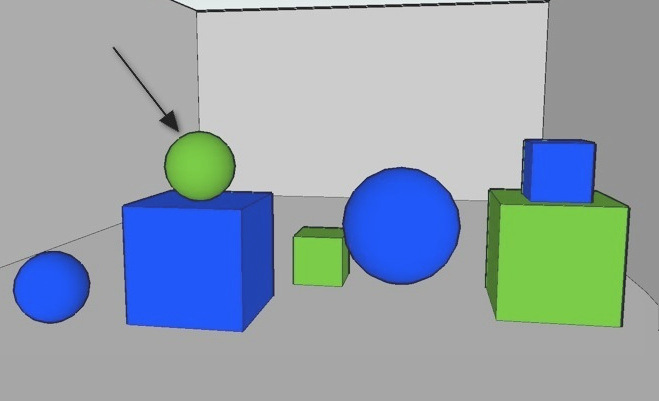
\includegraphics[width=.6\textwidth]{images/3.jpg}\\[0pt]
\label{fig-GRE3D7}
\caption{Imagen del GRE3D7 corpus.}\label{contexto-evaluacion}
\end{figure}

La \textbf{precisi\'on}  es una m\'etrica autom\'atica estricta que se puede usar para comparar rankings de ERS. Es la proporci\'on de coincidencias perfectas entre la salida de algoritmo y las ERs generadas por humanos y encontradas en corpora. 
La primer comparaci\'on de rankings de ERs se muestra en la Tabla \ref{results-algo-fig3}. Para cada ER, indicamos el n\'umero de veces que aparece en el corpus (\#Cor), la proporci\'on que representa (\%Cor), el n\'umero de veces que la gener\'o nuestro algoritmo (\#Alg) y la proporci\'on que representa (\%Alg).
Por \'ultimo, la precisi\'on (\%Acc) nos d\'a el porcentaje de aciertos de las ERs generadas por el algoritmo y se calcula como el m\'inimo entre el \%Cor y \%Alg. 

\begin{table}[H]
\begin{small}
\begin{center}
\begin{tabular}{|l|r|r|r|r|r|}
\hline
\multirow{2}{*}{Expresiones Referenciales} & \multicolumn{2}{|c|}{Corpus} & \multicolumn{2}{|c|}{Algoritmo} & Precisi\'on \\ \cline{2-6} 
 & \#Cor & \multicolumn{1}{|c|}{\%Cor} & \multicolumn{1}{|c|}{\#Alg} & \multicolumn{1}{|c|}{\%Alg} & \multicolumn{1}{|c|}{\%Acc} \\
\hline
ball, green                                    & 91 & 65.00 & 6376 & 63.76 & 63.76 \\
ball, green, small                              & 23 & 16.43 & 3440 & 34.40 & 16.43 \\
ball, green, small, ontop(blue, cube, large)      &  8 &  5.71 &    0 &  0.00 &  0.00\\
ball, green, ontop(blue, cube)                  &  5 &  3.57 &    0 &  0.00 &  0.00\\
ball, green, ontop(blue, cube, large)            &  5 &  3.57 &    0 &  0.00 &  0.00\\
ball, green, small, ontop(blue, cube)            &  2 &  1.43 &    0 &  0.00 &  0.00\\
ball, ontop(cube)                             &  1 &  0.71 &   27 &  0.27 &  0.27 \\
ball, green, small, ontop(blue, cube, large, left) &  1 &  0.71 &    0 &  0.00 &  0.00\\
ball, small, ontop(cube,large)	              &  1 &  0.71 &    2 &  0.02 &  0.02 \\
ball, green, top                                &  1 &  0.71 &    0 &  0.00 &  0.00\\
ball, small, ontop(cube)                       &  1 &  0.71 &    3 &  0.03 &  0.03 \\
ball, green, ontop(cube)                       &  1 &  0.71 &    0 &  0.00 &  0.00\\
ball, front, green                              &  0 &  0.00 &   97 &  0.97 &  0.00\\
ball, front, green, small                        &  0 &  0.00 &   13 &  0.13 &  0.00\\
ball, front, top                                &  0 &  0.00 &   12 &  0.12 &  0.00\\
ball, green, left	                              &  0 &  0.00 &   11 &  0.11 &  0.00\\
ball, top                                      &  0 &  0.00 &   10 &  0.10 &  0.00\\
ball, green, left, small                         &  0 &  0.00 &    5 &  0.05 &  0.00\\
ball, left, top                                 &  0 &  0.00 &    2 &  0.02 &  0.00\\
ball, small, top                                &  0 &  0.00 &    1 &  0.01 &  0.00\\
ball, front, ontop(cube, left)                  &  0 &  0.00 &    1 &  0.01 &  0.00\\

\hline
Total & 140 & 100 & 10000 & 100 & 80.51 \\
\hline
\end{tabular}
\caption{ERs del corpus, y las producidas por nuestro algoritmo para la Figura~\ref{contexto-evaluacion}.\label{results-algo-fig3}}
\vspace*{-.5cm}
\end{center}
\end{small}
\end{table}

 La precisi\'on del algoritmo con respecto al corpus GRE3D7 para esta escena es del 80\%. De las 14 ERs diferentes generadas por el algoritmo, 5 se encuentran en el corpus y las otras 9 no. Estas 9 expresiones referenciales incluyen propiedades de ubicación del target no con respecto a un landmark si no a su posición en la escena 3D. Por ejemplo \emph{la espera verde que está a la izquierda} se refiere a que la esfera verde está a la izquierda de la escena.  La probabilidad de uso de este tipo de propiedades es menor al 1 \%, en particular la de left es 0,007, pero, como esa probabilidad no es cero, dichas propiedades aparecen en ERs (siempre con menos de un 1% de frecuencia).  La m\'etrica de precisi\'on ha sido utilizada en trabajos anteriores para comparar la salida de un algoritmo de generaci\'on de ER con las ERs que se encuentran en corpora~\cite{sluis07:eval,viet:gene11} y se considera una m\'etrica muy estricta para esta tarea.

\subsection{Evaluaci\'on emp\'irica sobre el resto del corpus}
\label{sec:compara-varias}

Como es habitual cuando hacemos una evaluaci\'on con un caso particular, podemos pensar, que como el algoritmo tiene un componente de azar, por eso nos di\'o bastante bien, para esa ejecuci\'on particular. Por eso aqu\'i se muestra la misma comparaci\'on realizada en la secci\'on anterior pero con todas las im\'agenes verde-azules del corpus GRE3D7. 
Para enriquecer esta parte mostraremos otros baselines, los cuales dos dar\'an pistas de que las probabilidades de uso aprendidas con el m\'etodo que presentamos en esta tesis son \'utiles para aproximar al ranking de ERs que aparece en corpora. Los baselines que se presentan ejecutan el algoritmo con una distribuci\'on aleatoria de probabilidades de uso, y con una distribuci\'on uniforme (en las ERs tomando tanto las generadas por el sistema como las del corpus y las generadas como el modelo aleatorio). El Top baseline, es en el que el algoritmo us\'o las probabilidades de uso sacadas del corpus mismo. 

\begin{table}[h!]
\begin{small}
\begin{center}
\begin{tabular}{|l|c|c|c|c|}
\hline
         &  \puse\ de escena & \puse\ aprendidas & \puse\ random & uniforme \\ \hline
Escena 1	&	85.75\%	&	84.49\%	&	17.95\%	&	5.37\%	\\
Escena 3	&	82.81\%	&	80.51\%	&	9.89\%	&	4.40\%	\\
Escena 6	&	90.11\%	&	83.30\%	&	4.13\%	&	4.16\%	\\
Escena 8	&	86.52\%	&	64.06\%	&	16.32\%	&	9.75\%	\\
Escena 10	&	89.49\%	&	75.80\%	&	7.56\%	&	3.70\%	\\
Escena 12	&	80.21\%	&	81.29\%	&	57.09\%	&	6.68\%	\\
Escena 13	&	89.98\%	&	50.79\%	&	9.30\%	&	3.59\%	\\
Escena 21	&	92.13\%	&	80.01\%	&	8.45\%	&	6.77\%	\\
\hline
Promedio	&	87.13\%	&	75.03\%	&	16.34\%	&	5.55\%	\\

\hline
\end{tabular}
\caption{Precisi\'on entre las ERs del corpus y las generadas usando valores de \puse\ calculados desde la escena, aprendidos autom\'aticamente, provenientes de distribuciones random y uniformes.}\label{results-algo-all}
\end{center}
\end{small}
\end{table}


La primera columna muestra los valores obtenidos cuando corremos el algoritmo sobre la escena
con los valores de \puse\ obtenidos~\emph{de la propia escena}. Como se puede esperar,
esta columna tiene el mayor promedio de precisi\'on.

La segunda columna muestra los resultados del algoritmo cuando se ejecuta con \puse\ aprendido de
corpora como se explica en la Secci\'on~\ref{sec:learning} del cap\'itulo anterior. Este es el caso m\'as interesante porque muestra la capacidad de nuestra propuesta de generalizar a escenas no vistas con anterioridad y para las que no hay corpus. Para la mayor\'{i}a de las escenas la precisi\'on
es mayor al 80\% y la precisi\'on promedio es 75\%. La relativamente baja precisi\'on
obtenida en la escena 13 se explica principalmente las pobres estimaciones del valor de~\puse\ para las palabras \emph{large} y \emph{small} que son propiedades vagas y no absolutas ya que dependen de cu\'an grandes son en relaci\'on con los otros elementos del contexto.  

En el corpus, las relaciones \emph{large} y \emph{small} se utilizan mucho m\'as cuando el target no puede ser identificado usando s\'olo propiedades taxon\'omicas (\emph{ball} y \emph{cube}) y propiedades absolutas (\emph{green} y \emph{blue}), pero las caracter\'{i}sticas que hemos utilizado para el aprendizaje autom\'atico no capturan dichas dependencias como se discute en la Secci\'on \ref{sec:learning-corpus} del Cap\'itulo \ref{sec:algoritmo}.

A pesar de esta limitaci\'on, el promedio de la segunda columna es 75\%. Para una m\'etrica como la de precisi\'on que es considerada demasiado estricta, estos resultados son buenos. Adem\'as, el 25\% no cubierto por el algoritmo puede contener ERs igualmente buenas como evaluamos en la Secci\'on \ref{sec:humanevaluation}. Uno podr\'ia argumentar entonces que los valores de \puse\ aprendidos a partir del corpus son lo suficientemente buenos para ser utilizados para generar REs para nuevas escenas del dominio.

Las dos \'ultimas columnas pueden ser consideradas como baselines. En la primera generamos
valores aleatorios para \puse\. La precisi\'on obtenida es en la mayor\'{i}a de los casos pobre, pero con
una variaci\'on notable debido al azar. Adem\'as estas ejecuciones toman mucho m\'as tiempo en finalizar, lo que indica que se est\'an realizando demasiadas particiones sin conseguir llegar a la meta. Esta observaci\'on de performance es consistente con los resultados de los experimentos de generaci\'on humana realizados por \cite{keysar:Curr98,} y discutidos en la Seccion \ref{sec:psicolinguistica} del Cap\'itulo \refsec:seleccion}. Keysar argumenta que, las personas usan la prominencia de las propiedades en el dominio como heur\'istica para guiar la generaci\'on de ERs de forma de disminuir la carga cognitiva de tener que probar con todas las propiedades del dominio. Si la heur\'istica es buena, en muchos casos no es necesario ``revisar'' la ER para que identifique un\'ivocamente al target. Como efecto colateral de este proceso heur\'istico la ER resultante puede estar sobreespecificada, pero se genera r\'apidamente.  

Adem\'as de poca precisi\'on, cuando se utilizaron probabilidades random,  muchas de las ERs generadas suenan poco natural y son dif\'iciles de realizar sin introducir ambig\"uedades como, por ejemplo, (\textit{peque\~na cosa sobre
el cubo azul que est\'a abajo de algo que es peque\~no}). En la \'ultima columna se presenta la precisi\'on de una corrida artificial, le llamamos uniforme, uniforme tomando todas las ERs de las dem\'as columnas y asign\'andoles la misma probabilidad.
Para comparar nuestros resultados colos 3 baselines usamos tambi\'en entrop\'ia cruzada.
En teor\'ia de la informaci\'on, la \textbf{entrop\'ia cruzada} entre dos distribuciones de probabilidad mide la media de bits necesarios para identificar un evento de un conjunto de posibilidades, si un esquema de codificaci\'on est\'a basado en una distribuci\'on de probabilidad dada q, m\'as que en la verdadera distribuci\'on p. Vamos a comparar la entrop\'ia cruzada entre la distribuci\'on de probabilidad que se encuentra en el corpus, y la distribuci\'on de ER del corpus y las de ejecuciones del algoritmo con las probabilidades que acabamos de describir~(ver~\cite{juraksky:spee08} para obtener detalles sobre evaluaci\'on de entrop\'{i}a cruzada). En la Figura~\ref{Entropy} se muestran los resultados para las ocho escenas que hemos considerado.

\begin{figure}[ht]
\centering
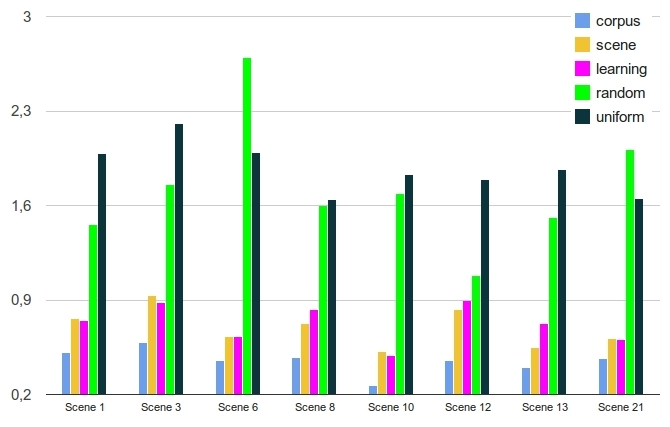
\includegraphics[width=0.6\textwidth]{images/entropy.jpg}
\caption{Entrop\'ia cruzada entre la distribuci\'on del corpus y diferentes ejecuciones del algoritmo.}\label{Entropy}
\end{figure}
  
Las entrop\'{i}as cruzadas de las dos primeras ejecuciones (\emph{escena} y \emph{aprendizaje autom\'atico}) son, en general, mucho m\'as cercanas de la entrop\'{i}a del corpus, que las entrop\'ias cruzadas de \emph{random} y \emph{uniforme}. S\'olo en la escena 12 random, por azar se acerca un poco m\'as.

%En esta secci\'on presentamos dos evaluaciones diferentes que realizamos en nuestro algoritmo. Secci\'on~\ref{sec:automaticevaluation} describe una evaluaci\'on con respecto al estado del arte~\cite{KrahmerGRAPH}. GRAPH fue el de mejor desempe\~no en las dos ediciones de la competencia ASGRE~\cite{gatt-balz-kow:2008:ENLG}. Debido a las limitaciones de los indicadores autom\'aticos, en la Secci\'on~\ref{sec:humanevaluation} realizamos una evaluaci\'on humana en la que pedimos a jueces humanos comparar la salida producida por nuestro algoritmo con las expresiones producidas por los seres humanos (las del corpus).


\section{Evaluaci\'on de rankings en el TUNA Challenge} \label{sec:automaticevaluation}

En esta secci\'on se presenta la comparaci\'on de nuestro algoritmo con el algoritmo que tuvo el mejor desempe\~no en el TUNA Challenge. 

\subsection{El TUNA Challenge}
El TUNA Challenge ...

El algoritmo GRAPH que describimos en el Cap\'itulo \ref{sec:seleccion} es un algoritmo determin\'stico y por lo tanto produce la misma expresi\'on referencial cuando se ejecuta con el mismo target y contexto. Nuestro algoritmo es no-determin\'istico, puede dar una expresi\'on referencial diferente cada vez que se ejecuta. Con el fin de compararlos corremos nuestro algoritmo 100 veces y hacemos un ranking de las 20 ERs ordenadas por la frecuencia que se produjeron. Utilizamos la parte de prueba del corpus TUNA (el cual fue introducido en la Secci\'on \ref{sec:corpusTUNA}), para comparar el ranking de ERs dado por nuestro algoritmo con las salidas del algoritmo GRAPH cuyos resultados se describen en~\cite{KrahmerGRAPH} y se reproducen en la Tabla~\ref{Tabla_sis_1_20}.


\subsection{Comparaci\'on con el TUNA Challenge}
El algoritmo GRAPH define la generaci\'on de expresiones referenciales como un problema de b\'usqueda en un grafo, devuelve el grafo distintivo de menor costo (si existe) dada una funci\'on de costo particular. Comparamos a este algoritmo usando las m\'etricas precisi\'on, Dice y \textsc {masi}, introducidas en la Secci\'on \ref{sec:metricasAutomaticas}. 

Recordemos que el corpus TUNA tiene 2 partes, una parte cuyo dominio son muebles, y otra parte cuyo dominio son personas, ambos ubicados en una grilla. Para realizar esta comparaci\'on se us\'o s\'olamenta la parte singular del corpus.

En la Tabla~\ref{Tabla_sis_1_20} mostramos m\'etricas autom\'aticas y comparamos la performance de nuestro sistema con el sistma GRAPH para la primer ER en el ranking y para las primeras 20 ERs del ranking.

\begin{table}[H]
\begin{center}
\begin{tabular}{|l|c|c|c|}
\hline
%Figure & Model \puse &  Learning \puse & Random \puse &  Uniform \puse \\
	 	& 	Dice		&	\textsc{masi}	&	Precisi\'on		\\
\hline
sistema GRAPH, Dominio muebles	& 	80\% 		&	59\%	&	48\%		 	\\
sistema GRAPH, Dominio personas 	& 	72\%		&	48\%	&	28\%			\\
\hline
Nuestro sistema, Dominio muebles (top 1)	&	80\%		&	60\%	&	47\%		\\
Nuestro sistema, Dominio personas (top 1)	&	65\%		&	37\%	&	19\%		\\
\hline
Nuestro sistema, Dominio muebles (top 20)&	87\%		&	75\%  	&	65\%		\\
Nuestro sistema, Dominio personas (top 20)   &	81\%		&68\%	&	60\%		\\
\hline
\end{tabular}
%\vspace*{.1cm}
\caption{Comparaci\'on del algoritmo GRAPH y nuestro sistema. Consideramos 3 m\'etricas autom\'aticas para el top 1 y para el top 20 ERs producidas por nuestro algoritmo.}
%\vspace*{-.5cm}
\label{Tabla_sis_1_20}
\end{center}
\end{table}
%\vspace*{-.5cm}
%Accuracy, Dice and \textsc{masi} assess humanlikeness with respect to a corpus of human referring expressions. In the Figure~\ref{graficoPresicion} the accuracy for our system and the GRAPH system is compared. The left GRAPH corresponds to the furniture domain and the right GRAPH corresponds to the people domain. We can see that taking the top 1 ER our system accuracy is lower than GRAPH performance for the people domain. However, if we consider the top 20 REs that our algorithm is able to produce we can see that the accuracy for both domains gets higher than 60\%. This shows that our algorithm is able to generate REs that are more similar to those produced by humans than the GRAPH algorithm, although these REs are not ranked first. 

%Another result that we can observe is that the people domain accuracy is much lower for the top 1 ER than for the furniture domain (19 vs 47), but the accuracy stabilizes when REs lower in our ranking are considered. This may be explained by the fact that the training set for the people domain is smaller and less balanced and hence, the probabilities of use inferred do not generalize as well as in the furniture domain. 

%\hline
%Precisi\'on, Dice y \textsc{masi}  evaluar humanlikeness con respecto a un corpus de expresiones humanas en referencia.
En la Figura~\ref{graficoPresicion} se muestra una comparaci\'on entre la precisi\'on de nuestro sistema y el sistema GRAPH. El gr\'afico de la izquierda corresponde al dominio muebles y el gr\'afico de la derecha corresponde al dominio personas. En el dominio muebles estamos obteniendo casi los mismos n\'umeros en las m\'etricas evaluadas.
Podemos ver que si tomamos la parte superior, es decir 1 ER (la primera, la m\'as probable), nuestra precisi\'on es menor que de GRAPH para el dominio de las personas. Sin embargo, si tenemos en cuenta las 20 mejores ERs que nuestro algoritmo es capaz de producir, podemos ver que la precisi\'on para ambos dominios se hace mayor del 60\% (60\% para personas y 65\% para muebles). Esto demuestra que nuestro algoritmo es capaz de generar ERs que son m\'as similares a las producidas por los seres humanos que el algoritmo GRAPH, aunque estas ERs no esten en primer lugar. Si el algoritmo GRAPH fuera modificado para ser no-determin\'istico es posible que tambi\'en mejorara su precisi\'on en 20 o m\'as ejecuciones. Esta es una l\'inea interesante de trabajo futuro. 

\begin{figure}[H]
\begin{minipage}{0.50\linewidth}
\centering
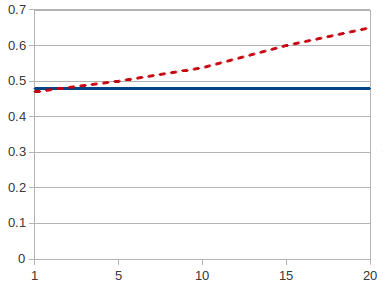
\includegraphics[width=\textwidth]{images/furniturePrec.png}
\caption{Muebles.}
%\end{figure}
\end{minipage}
%\begin{figure}[ht]
\begin{minipage}{0.50\linewidth}
\centering
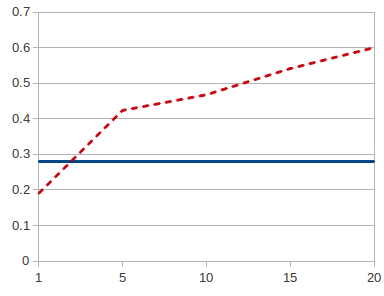
\includegraphics[width=\textwidth]{images/precP.png}
\caption{Personas.}
\end{minipage}
\caption{Comparaci\'on de la precisi\'on  del algoritmo GRAPH y nuestro sistema. El eje x indica que la precisi\'on se calcul\'o teniendo en cuenta las x primeras ER en el ranking. El eje y indica la precisi\'on . Nuestro sistema es representado como una l\'inea de puntos y GRAPH como una l\'inea continua.\label{graficoPresicion}}
\end{figure}

Otro resultado que podemos observar es que la precisi\'on  del top 1 en el dominio personas es mucho menor (19\%) que para el dominio de muebles (47\%), pero la precisi\'on se estabiliza cuando se consideran m\'as ERs de nuestro ranking. Esto puede explicarse por el hecho de que el conjunto de el dominio de personas contiene muchas m\'as propiedades que se pueden elegir para describir a las personas que las que contiene el dominio de muebles.

Normalmente las m\'etricas autom\'aticas tienen la desventaja de calificar como malas a ERs que son buenas ERs, es decir identifican el target un\'ivocamente, en el contexto considerado, pero las consideran malas por no ser exactamente como las que aparecen en corpora. Otra manera de evaluar qu\'e tan buena es una ER es con evaluaciones manuales. Mostraremos una evaluaci\'on humana en la siguiente secci\'on.

 
%\vspace*{-1.0cm}

\section{Evaluaci\'on humana} \label{sec:humanevaluation}

%We asked two native speaker judges of English to evaluate our referring expressions via an experiment on the web. The authors of the paper did not participate during the evaluation. The judges could register to the evaluation system so that they did not have to complete it in one go, the could come back to it later. During the evaluation we showed each judge the scenes and two randomly ordered REs. One ER corresponded to the ER present in the corpus and produced by a person and the other ER corresponded to the top 1 ER produced by our system. We asked the judges to select the ER that would be more useful to identify the target in the scene. That is, to select it from among the other objects in the stimulus pictures. 

%Our goal is to show that even if the ER generated by our algorithm does not coincide with the ER produced by a human in the corpus collection, it can be judged as good or even better than the REs generated by humans. 

%In Table~\ref{system-versus-human} we show the results from the human evaluation experiment.
%The REs produced by the system were considered equal or better by both
%judges in 60 \% of the cases and, by at least one judge in 92\% of the cases.


En las secciones anteriores describimos evaluaciones autom\'aticas de nuestro algoritmo. En esta secci\'on explicamos una evaluaci\'on humana que hicimos de las ERs generadas por nuestro algoritmo con las probabilidades de uso aprendidas para el TUNA corpus y descriptas en la secci\'on anterior.  

Como las ERs que generamos las generamos para el idioma ingl\'es, pedimos a dos jueces nativos de Ingl\'es evaluar nuestras expresiones referenciales a trav\'es de un experimento en la web. Los jueces podr\'{i}an entrar en el sistema de evaluaci\'on varias veces, es decir no ten\'ian que terminar la evaluaci\'on en la primera vez, para cada ER pod\'ian resolverla o pod\'ian volver a ella m\'as tarde. 

Durante la evaluaci\'on mostramos a cada juez una escena y dos ERs ordenadas al azar. Una ER correspond\'ia a la ER presente en el corpus TUNA producida por una persona para la escena y la otra ER correspond\'ia a la ER producida por nuestro sistema. Solicitamos a los jueces seleccionar la ER que ser\'{i}a m\'as \'util para identificar el target en la escena. El juez pod\'ia elegir una ER o indicar que las 2 ER le parec\'ian igualmente buenas.

Nuestro objetivo es mostrar que incluso si la ER generada autom\'aticamente no coincide con la ER producida por un ser humano del corpus, puede ser juzgada como buena o incluso mejor que la ER generada por una persona.

En la Tabla~\ref{system-versus-human} se muestran los resultados del experimento de evaluaci\'on humana.
Las ERs producidas por el sistema en el top 1 fueron consideradas igual o mejor por los 2 jueces que las generadas por personas en el 75\% de los casos para los muebles y en el 43\% para las personas. Esto contrasta con el 47\% para personas y 19\% para muebles de la Tabla \ref{Tabla_sis_1_20}. Esto muestra que la m\'etrica de precisi\'on es demasiado estricta para la tarea, y las m\'etricas de DICE o masi se acercan m\'as a evaluaciones humanas. Adem\'as al menos 1 juez consider\'o que el 97\% de las ERs del sistema eran tan buenas o mejores que las humanas para los muebles y (87\% para las personas). Esto muestra que la evaluaci\'on de la calidad de las ERs es parcialmente subjetiva. S\'olo en el 8\% de los casos ambos jueces coincidieron que una ER generada autom\'aticamente era peor que la humana.

\begin{table}[h!]
\begin{center}
\begin{tabular}{|l|c|c|c|}
\hline
%total scenes in evaluation set &                           80   &             68
 & Dominio muebles & Dominio personas & Media ponderada \\
\hline
%sistema igual al humano  	&	.46	&	.19	&	.33 \\
%sistema mejor por 2 jueces &	.29 	& 	.24 	& 	.27 \\
%sistema mejor por 1 or 2 jueces & .51	&	.68	&	.59 \\
sistema igual o mejor por 2 jueces  &.75  &       .43	&       .60 \\
sistema igual o mejor por 1 juez  &.97	&	.87	&	.92 \\
sistema peor por 2 jueces &	.03	&	.13	&	.08 \\
\hline
\end{tabular}
%\vspace*{.1cm}
\caption{Comparaci\'on de ERs generadas por personas y por nuestro algoritmo para el corpus TUNA.} 
\label{system-versus-human}
\vspace*{-.5cm}
\end{center}
\end{table}

%Below, we illustrate the evaluation experiment by showing examples of cases in which the system expression was considered better by both judges, by only one judge or by neither of them. 

%Figure~\ref{smallBlueFan} illustrates a case in which the human generated an underspecified ER while the system produced an ER which unequivocally identifies the target. The ER generated by the system for this figure is ``small blue fan'' while the ER produced by the human is ``blue fan''. The human ER fails to uniquely identify the target and is then not preferred by the human judges. Humans are known for producing underspecified REs which may be due to cognitive limitations for not being able to consider the whole referential context at the same time. Our algorithm is able to consider the whole referential context and combine this ability with the probability of use of the REs learned from humans. 

A continuaci\'on, se ilustra el experimento de evaluaci\'on, mostrando ejemplos de casos en los que la expresi\'on del sistema fue considerada mejor por ambos jueces, por un solo juez o por ninguno de los dos.

Figura~\ref{smallBlueFan} ilustra un caso en el que el humano genera una ER subespecificada mientras que el sistema produce un ER que identifica de manera inequ\'{i}voca al target. La ER generada por el sistema para esta figura es {\it peque\~no ventilador azul}, mientras que la ER producida por el ser humano es {\it ventilador azul}. La ER del humano no logra identificar de forma \'unica el target y entonces no es preferida por los jueces humanos. Los seres humanos son conocidos por producir ERs subespecificadas, esto puede ser debido a las limitaciones cognitivas por no ser capaz de considerar todo el contexto referencial al mismo tiempo. Nuestro algoritmo es capaz de considerar todo el contexto referencial y combinar esta capacidad con la probabilidad de uso de las ERs aprendidas de los seres humanos.




\begin{figure}[h]
\begin{minipage}{0.48\linewidth}
\centering
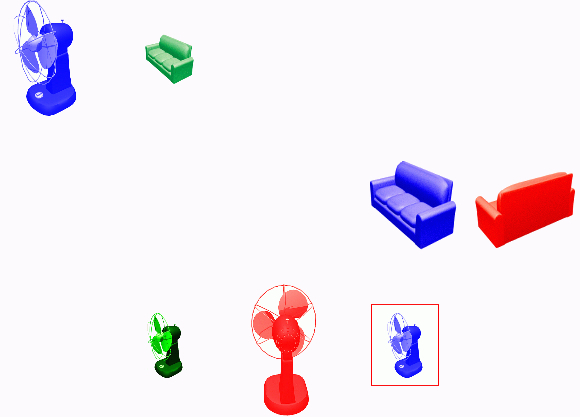
\includegraphics[width=\textwidth]{images/smallBlueFan.jpg}
\caption{Escena usada durante la recolecci\'on del TUNA corpus. La ER humana \emph{ventilador azul}, y la del sistema \emph{ventilador azul peque\~no}. Los jueces prefirieron la ER generada por el sistema.}
\label{smallBlueFan}
\end{minipage}
\hspace*{.04cm}
\begin{minipage}{0.48\linewidth}
\centering
\vspace*{.4cm}
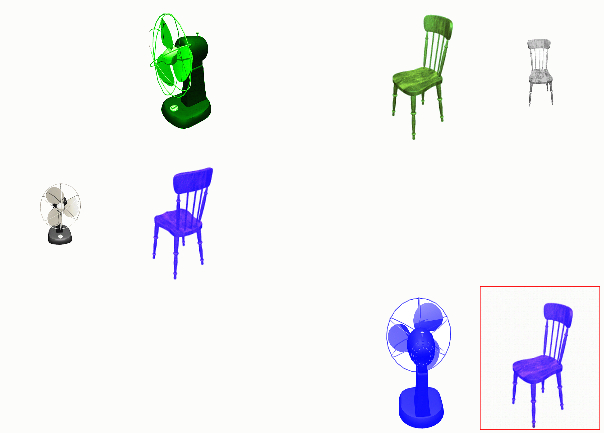
\includegraphics[width=\textwidth]{images/tuna.jpg} % esta es la 101t5 la que mostramos al principio
\vspace*{-.4cm}
\caption{Escena usada durante la recolecci\'on del TUNA corpus. La ER humana \emph{silla azul frontal}, y la del sistema \emph{La silla azul de abajo}. Ambos jueces humanos prefirieron la generada por el sistema.}
\label{BlueChair}
\end{minipage}
\end{figure}


%In Figure~\ref{BlueChair} the human ER was ``blue frontal chair'', and the system ER was ``the blue chair in the bottom''; both judges selected the system RE. This case can be explained by the fact that, in this domain, the property ``bottom'' helps more during the identification than the property ``frontal'' because it concentrates the attention of the interpreter in the lower part of the scene. Our system learns this fact by learning a higher value of \puse~for ``bottom'' than for ``frontal'' from the training data. 

En la Figura~\ref{BlueChair} la ER humana era {\it silla frontal azul}, y la ER sistema era {\it la silla azul de abajo}; ambos jueces seleccionaron la ER sistema. Este caso se puede explicar por el hecho de que, en este \'ambito, la propiedad {\it abajo} ayuda m\'as durante la identificaci\'on de la propiedad {\it frontal} porque concentra la atenci\'on del interlocutor en la parte inferior de la escena. Nuestro sistema aprende este hecho por el aprendizaje de un mayor valor de \puse\ para {\it abajo} que para {\it frontal} a partir de los datos de entrenamiento.

\begin{figure}[h]
\begin{minipage}{0.48\linewidth}
\centering
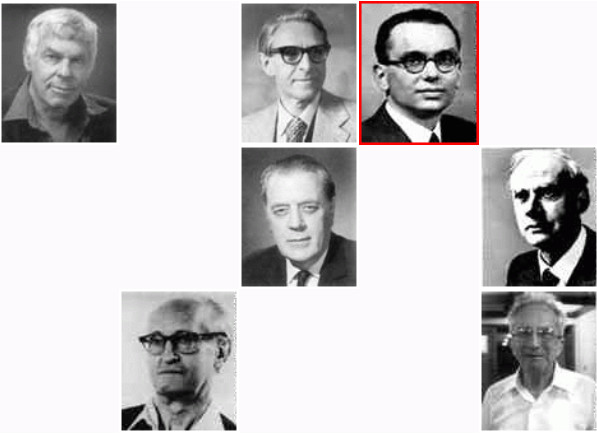
\includegraphics[width=\textwidth]{images/s59t26.jpg}
\caption{Escena usada durante la recolecci\'on del TUNA corpus. La ER humana \emph{the man with black hair}, y la del sistema \emph{the man wearing glasses in the fourth column}. Los jueces prefirieron la ER humana.}
\label{s28t25}
\end{minipage}
\hspace*{.04cm}
\begin{minipage}{0.48\linewidth}
\centering
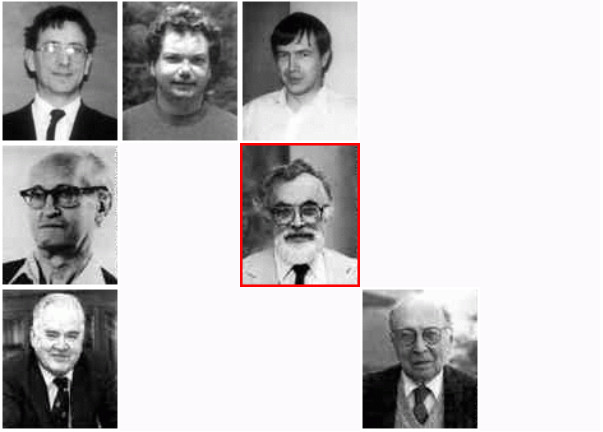
\includegraphics[width=\textwidth]{images/s315t21.jpg}
\vspace*{-.3cm}
\caption{Escena usada durante la recolecci\'on del TUNA corpus. La ER humana \emph{man with a beard},  y la del sistema \emph{man with a beard wearing glasses}. Los jueces no estuvieron de acuerdo en su preferencia.}
\label{s307t21}
\end{minipage}
\end{figure}

%Figure~\ref{s28t25} is an example for which both judges preferred the human expression. The human  ER was ``the man with black hair'', and the system's ``the man wearing glasses in the fourth column''. This example makes evident the fact that, in the people domain some properties are more salient in some images than in others because of different shades of colors. Gradable properties such as this ones (in contrast to absolute properties) are still an open problem for GRE algorithms. 

%Figure~\ref{s307t21}~illustrates a case in which the system ER was more overspecified than the human RE; the system included ``wearing glasses'' while the human did not. In this case one human subject preferred the system ER and the other the human RE. The amount of overspecification is a subjective matter where human themselves disagree. Further evaluation where REs are actually used for a task would be interesting to investigate this issue.  


Figura~\ref{s28t25} es un ejemplo en el que ambos jueces prefirieron la expresi\'on humana. La ER humana era {\it el hombre con el pelo negro}, y del sistema de {\it el hombre con gafas en la cuarta columna}. Este ejemplo pone de manifiesto el hecho de que, en el dominio de las personas algunas propiedades son m\'as destacadas en algunas im\'agenes que en otrosadebido a diferentes tonos de colores. Propiedades graduables como estas (en contraste con las propiedades absolutas) son todav\'{i}a un problema abierto para los algoritmos de GER.

Figura~\ref{s307t21}~ilustra un caso en el que la ER del sistema era m\'as sobreespecificada que la ER humana; el sistema incluye {\it con gafas}, mientras que el ser humano no lo hizo. En este caso un sujeto humano prefiere la ER del sistema y el otro la ER del humano. La cantidad de sobreespecificaci\'on es una cuesti\'on subjetiva, donde los humanos mismos no est\'an de acuerdo. Una evaluaci\'on donde las ERs se utilicen para resolver una tarea ser\'{i}a interesante para investigar este asunto.

\section{}




\chapter{Conlusiones}
\label{sec:conclusiones}
\include{principal/7_conlusiones}

\vskip 0.2in
\bibliography{bibliografia}
\bibliographystyle{theapa}
\end{document}

%\chapter{Introducci\'on}
%\label{ch:intro}
%\chapter{Introducci\'on}
\label{sec:intro}
%tesis en linguistica http://elies.rediris.es/miscelanea/misce_9/alcina.pdf

%En este cap\'itulo daremos una introducci\'on al problema de la generaci\'on autom\'atica de expresiones referenciales, contaremos las contribuciones de este trabajo y mostraremos como est\'a organizada la tesis.


La {\bf generaci\'on de lenguaje natural (GLN)} es el proceso autom\'atico (o semi autom\'atico) de construcci\'on de un texto en lenguaje natural, para la comunicaci\'on con fines espec\'ificos. Este proceso que convierte informaci\'on a texto en lenguaje natural, es \'util para aplicaciones pr\'acticas en las que, por ejemplo, es necesario hacer accesible grandes vol\'umenes de informaci\'on posiblemente t\'ecnica. La GLN se ha usado para generar recomendaciones de restaurantes personalizadas, para resumir informaci\'on m\'edica, etc.~\cite{dale2000}. La generaci\'on de lenguaje natural, est\'a dentro del \'area de procesamiento del lenguaje natural, que es una rama principal de la inteligencia artificial.

Una {\bf expresi\'on referencial (ER)} es un sintagna nominal que identifica un\'ivocamente a un objeto en un contexto y para un interlocutor particular. Si quisi\'eramos referirnos al objeto se\~nalado por la flecha en la Figura~\ref{GRE3D7-stimulus1}, podr\'iamos hacerlo con alguna de las expresiones referenciales que se muestran en la Figura \ref{er-figura1}.

\begin{figure}[h]
\begin{subfigure}{.5\textwidth}
  \centering
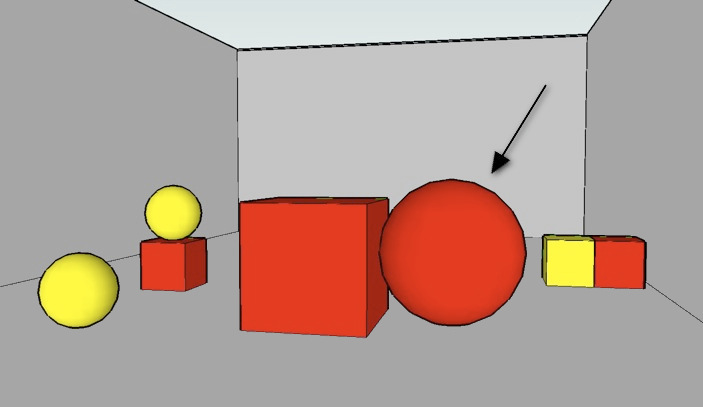
\includegraphics[width=\textwidth]{images/22sinletrasClaro.jpg}
  \caption{}\label{GRE3D7-stimulus1}
\end{subfigure}%
\begin{subfigure}{.5\textwidth}
 \centering
\begin{tabular}{l}
 {\it La esfera grande}\\

 {\it La esfera roja que est\'a al lado del cubo rojo} \\

 {\it El objeto que est\'a al lado del cubo grande}\\

 {\it La bola roja}\\

 {\it La pelota a la izquierda del cubo amarillo}\\

 {\it La bola grande}\\

 {\it La esfera que est\'a a la derecha del cubo rojo y a }\\
{\it la izquierda del cubo amarillo}\\

 {\it La cosa que est\'a a la derecha del cubo del medio}\\

  {\it ...}
 \end{tabular}
\hspace*{-30cm}
\centering\caption{}\label{er-figura1}
\end{subfigure}
\begin{centering}
\caption{Expresiones referenciales que identifican al objeto se\~nalado por la flecha.}
\label{figura-er}
\end{centering}
\end{figure}

La \textbf {generaci\'on de expresiones referenciales (GER)} entre todas las subtareas de GLN, es una de las que ha recibido m\'as atenci\'on. En la pr\'actica, la mayor\'ia de los sistemas de GLN, con independencia de su finalidad, contiene un m\'odulo de GER de alg\'un tipo~\cite{Mellish2004}. Esto no es sorprendente
en vista del papel central que las expresiones referenciales tienen en la comunicaci\'on. Un sistema que proporciona
consejos sobre los viajes a\'ereos \cite{white2010generating} tiene que hacer referencia a los vuelos ---{\it el vuelo m\'as barato}, {\it un vuelo directo}---, un sistema de navegaci\'on para autom\'oviles~\cite{Drager:2012:GLN:2380816.2380908}
necesita generar descripciones espaciales ---{\it tomar el puente junto a la iglesia, a la derecha}---,
y un robot que ensambla piezas de juguetes junto con un usuario humano~\cite{foster-etal-ijcai2009} debe hacer referencia a los componentes ---{\it inserte el perno verde hasta el final en el cubo rojo}. Cuando hablamos, nos referimos a cosas (tangibles como un puente, o intangibles como una fecha), es decir generamos expresiones referenciales. Un sistema que genera texto, tambi\'en deber\'a generar expresiones referenciales. La generaci\'on autom\'atica de expresiones referenciales es el tema de esta tesis.

Un sistema de GLN incluye 3 etapas: {\bf determinaci\'on de contenido} ---qu\'e decir--- {\bf lexicalizaci\'on} ---con qu\'e palabras--- y {\bf realizaci\'on ling\"{u}\'istica} ---c\'omo decirlo. La determinaci\'on de contenido, elige qu\'e informaci\'on incluir en la oraci\'on. La lexicalizaci\'on elige qu\'e lexemas usar para comunicar el contenido determinado por la etapa anterior. Y la realizaci\'on arma la oraci\'on agregando los art\'iculos, preposiciones, y dem\'as palabras funcionales necesarias y orden\'andolas de forma tal que la frase resultante sea gramaticalmente aceptable. 

Un sistema de GER, tiene esas 3 etapas tambi\'en: {\bf determinaci\'on de contenido} ---decide qu\'e propiedades o relaciones del objeto a describir se incluir\'an en la expresi\'on referencial--- {\bf lexicalizaci\'on} ---elige las palabras que se van a usar para nombrar las propiedades y relaciones--- y {\bf realizaci\'on ling\"u\'istica} ---se encarga de armar el sintagma nominal para que sea gramaticalmente correcto.

Por ejemplo, la primer ER de la Figura \ref{figura-er} incluye las propiedades {\it tama\~no} y {\it forma} del objeto se\~nalado por la flecha, lexicalizadas como {\it grande} y {\it esfera} respectivamente y realizadas agregando el art\'iculo {\it la} antes de {\it esfera}, e incluyendo el sustantivo {\it esfera} antes que el adjetivo {\it grande}; formando as\'i el sintagma nominal {\it La esfera grande} que es correcto en espa\~nol. Otra lexicalizaci\'on y realizaci\'on de las mismas propiedades ---es decir, de la misma sem\'antica--- podr\'ia ser {\it La bola de gran tama\~no}. A lo largo de esta tesis usaremos el t\'ermino {\bf expresi\'on referencial} (ER) para nombrar la salida de cualquiera de las 3 etapas de la GER. Es decir, llamaremos expresi\'on referencial al conjunto de propiedades y relaciones que refieren un\'ivocamente a un objeto aunque no est\'en lexicalizadas o realizadas.

En lo que sigue introduciremos terminolog\'ia b\'asica, relacionada con la GER que nos servir\'a a lo largo de toda la tesis para entendernos.

El {\bf dominio} de una ER define los tipos de entidades que est\'an siendo contemplados. Por ejemplo el dominio de la Figura \ref{figura-er} son las figuras geom\'etricas en 3 dimensiones. En particular, el dominio incluye cubos y esferas de colores rojo y amarillo, algunas grandes y otras peque\~nas, situadas en un entorno con perspectiva.

El {\bf contexto} de una ER contiene un subconjunto de las entidades del dominio. La Figura \ref{figura-er} muestra un contexto con 7 entidades del dominio, 4 rojas y 3 amarillas. Otros ejemplos son los puntos de referencia visibles en un cierto momento en un camino para el que estamos dando direcciones, un subconjunto de las fotograf\'ias utilizadas en una configuraci\'on experimental, o los ingredientes de cocina que ya se han mencionado en una receta. En un dominio visual, el contexto, incluyendo las propiedades de sus objetos y su configuraci\'on espacial, se puede llamar \textbf{escena}. %El contexto de la Figura \ref{GRE3D7-stimulus1} son los todos los objetos visibles con sus propiedades.

Cada {\bf entidad} del contexto (tambi\'en conocido como objeto o elemento) tiene un tipo ---\emph{esfera}--- ciertas propiedades o caracter\'isticas ---\emph{color}---, valores de esas propiedades ---\emph{rojo}---, y puede tener relaciones con otros objetos ---\emph{a la derecha de}. Una {\bf propiedad} (unaria) es una caracter\'istica de una entidad particular. Por ejemplo, la raza de un perro, el tener o no tener bigotes para un hombre, o el color para un objeto. Cada entidad puede tener muchas propiedades, y puede tener relaciones (tambi\'en llamadas: propiedades binarias), por ejemplo con respecto a la posici\'on f\'isica, como estar situado al lado de otro objeto. 

El {\bf target} (u objetivo), es el subconjunto de objetos de un contexto a los cuales queremos referirnos. En la escena del ejemplo de la Figura \ref{figura-er}, el target es el objeto se\~nalado por la flecha. En este caso, el target es un conjunto singleton, es decir tiene un s\'olo elemento. Si el target tiene m\'as de un elemento, las ERs que lo identifican son plurales.

Dado un contexto, un target y una descripci\'on (parcial) del target, los {\bf distractores} son otros elementos que se encuentran en el contexto, y que tambi\'en cumplen con la descripci\'on parcial. Si la descripci\'on parcial es {\it esfera} las esferas que no son el target de la Figura \ref{figura-er} son  distractores, y por ello es necesario seguir agregando propiedades o relaciones para identificar un\'ivocamente al target.

Un {\bf algoritmo} para GER, es un procedimiento autom\'atico que toma, al menos, alg\'un tipo de representaci\'on de un contexto y un target, y da como resultado una (o m\'as) expresi\'on(es) referencial(es) para el target considerado, si puede identificarlo un\'ivocamente en el contexto.

Una computadora que se enfrenta a la tarea de generar autom\'aticamente expresiones referenciales en un contexto determinado, necesitar\'a una representaci\'on de todos los objetos de la Figura \ref{figura-er} y las propiedades de cada uno de ellos. En la Figura~\ref{contexto-tabla-propiedades} se muestra una posible forma de representar los objetos, sus propiedades y relaciones: una base de datos que contiene todas las propiedades relevantes de los objetos de la escena. Entonces, la tarea de GER para el objeto $e_5$ involucra encontrar alguna combinaci\'on de valores de propiedades y relaciones con otros objetos, que aplique \'unicamente a $e_5$, y no a los otros objetos. Como dijimos, esta tarea de encontrar las propiedades y relaciones que aplican a un target y no a los distractores, se llama {\emph selecci\'on de contenido para la generaci\'on de una expresi\'on referencial}. Mirando la Tabla \ref{tabla-propiedades} podemos decir que {\it red ball}, {\it large ball} y {\it large red ball} son algunas ERs del objeto $e_5$, cuyas realizaciones en espa\~{n}ol podr\'ian ser: {\it La bola roja}, {\it La esfera grande} y {\it La esfera grande y roja}. {\it La bola roja} y {\it La esfera grande} aparecen entre las ERs dadas por las personas listadas en la Figura \ref{figura-er}.
%Como una primera intuici\'on podemos ver que la Figura \ref{formula-subgrafo} es un subrafo de la Figura \ref{representacion-modelo} que identifica un\'ivocamente al target, representa la cuarta ER mostrada en la Figura \ref{er-figura1}. Y la Figura \ref{formula-subgrafo2} tambi\'en identifica al target un\'ivocamente y representa la segunda ER mostrada en \ref{er-figura1}.
%que est\'an dadas en la Figura \ref{er-figura1} son muchas m\'as de las que mostramos en las f\'ormulas de la Figura \ref{er-figura1-b}, esto nos lleva a pensar que un algoritmo puede que no consiga la variedad que las personas dan. La representaci\'on ilustrada en la Figura~\ref{representacion-modelo} es equivalente a la mostrada en la Tabla \ref{tabla-propiedades}.

%\vspace*{-1.5cm}
\begin{figure}[h]
\begin{subfigure}{.45\textwidth}
  \centering
	\vspace*{-.2cm}
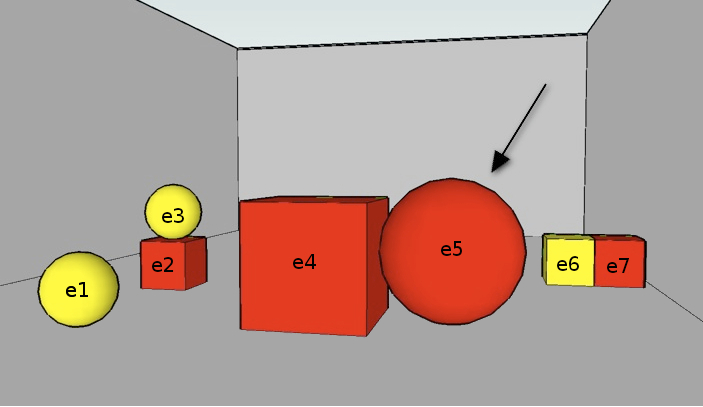
\includegraphics[width=\textwidth]{images/22.jpg}
  \caption{}\label{GRE3D7-stimulus1-ids}
\end{subfigure}
\begin{subfigure}{1\textwidth}
% \centering
%\begin{centering}
\hspace*{-16cm}
\begin{scriptsize}
\begin{tabular}{|l|c|c|c|c|c|c|c|}
\hline
\textbf {id}& 	\textbf {type}		&	\textbf {color}	&	\textbf {size}& \textbf {rigth} & \textbf {left} & \textbf {ontop}	& \textbf {below}	\\
   	   &  	    			&	    		&	     		&  \textbf {of}   		 &  \textbf {of}	    &  	&  \\
\hline \hline
$e_1$ & ball & yellow & small & - & - & - & - \\
$e_2$ & cube & red & small & - & - &- & $e_3$ \\
$e_3$ & ball & yellow & small & - & - & $e_2$ & -\\
$e_4$ & cube & red & large & - & $e_5$ & - & -\\
$e_5$ & ball & red & large & $e_4$ & - & - & -\\
$e_6$ & cube & yellow & small & - & $e_7$ & - & -\\
$e_7$ & cube & red & small & $e_6$ & - & - & -\\
\hline
%&&&&&&&\\
%&&&&&&&\\

\end{tabular}
\end{scriptsize}
\vspace*{1cm}
%\center
\centering \hspace*{-8cm} \caption{}\label{tabla-propiedades}
%\end{centering}
\end{subfigure}
\caption{Formalizaci\'on de las propiedades de la escena en una tabla de doble entrada.}\label{contexto-tabla-propiedades}
\end{figure}

En la pr\'oxima secci\'on veremos porqu\'e la tarea de GER es m\'as compleja de lo que parece a primera vista y en la siguiente introduciremos c\'omo herramientas de teor\'ia de modelos nos pueden ayudar.

\section{Expresiones referenciales bajo incertidumbre}
\label{sec:gre-incertidumbre}


%Los conjuntos son dif\'icil para referirse a, por ejemplo, y algoritmos
%diseñado para tratar con ellos lograr una menor semejanza humana cuando se refiere a los conjuntos de
%a los objetos individuales (van Deemter et al., en prensa). Los recientes esfuerzos para dejar que los algoritmos REG
%referirse a las regiones espaciales sugieren que en dominios grandes, realista, identificación precisa de
%un objetivo es un objetivo que se puede aproximar, pero rara vez alcanzado (Turner et al., 2008;
%Turner, Sripada, y Reiter 2009) .Es en tales dominios que prominencia (especialmente en el
%sentido no lingüístico) se convierte en un problema crítico. 
Cuando la generaci\'on de expresiones referenciales ocurre en la vida real, en lugar de ocurrir en un experimento controlado, las fuentes de \textbf{incertidumbre} que afectan al proceso se multiplican. En trabajo 
reciente en el \'area de GER \cite{turner2008,turner2009} se discute que, al intentar usar algoritmos de GER en dominios grandes 
y realistas (como por ejemplo la descripci\'on de regiones en mapas) la identificaci\'on precisa del target es una tarea que puede ser 
aproximada pero raramente lograda. Los autores argumentan que esto se debe, en parte, a que las representaciones geogr\'aficas 
son necesariamente \textbf{incompletas}. Esta falta de informaci\'on introduce incertidumbre (por ejemplo, el restaurante se\~nalado por la flecha en la Figura \ref{target_mapa}, ?`es realmente el \'unico restaurante de esa calle? o ?`es el \'unico que aparece en el mapa?).

\begin{figure}[h]
\centering
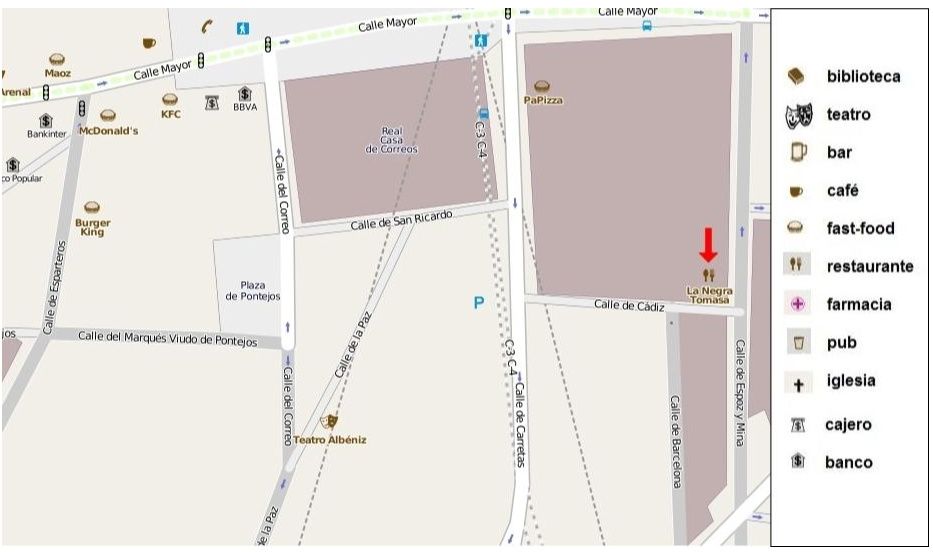
\includegraphics[width=\textwidth]{images/corpus/mapa15.png}
\caption{Ejemplo de target en el contexto de un mapa del ZOOM corpus.}
\label{target_mapa}
\end{figure}

Cuando la informaci\'on del contexto proviene de datos de sensores, las entradas del algoritmo de GER son inevitablemente ruidosas. Es decir, 
contienen informaci\'on no s\'olo incompleta sino tambi\'en posiblemente {\bf incorrecta}. Incluso en contextos tan simples como el de la 
Figura \ref{figura-er} hay incertidumbre. ?`La Figura \ref{representacion-modelo1} representa toda la informaci\'on del 
contexto?. Algunos podemos opinar que s\'i, otros que no. 

\begin{figure}[h]
%\begin{subfigure}{.5\textwidth}
  \centering
\vspace*{1cm}
\begin{picture}(250,50)
\put(0,-50){\begin{tikzpicture}
  [
    n/.style={circle,draw,inner sep=1.5pt,node distance=1.5cm},
		 aArrow/.style={->, >=stealth, semithick, shorten <= 1pt, shorten >= 1pt},
  ]
 \node[n,label=below:{
    \relsize{-2}$\begin{array}{c}
      \nSmall\\[-3pt] 
      \nYellow \\[-3pt] 
      \nBall\end{array}$}] (a) {$e_1$};
 \node[n,label=below:{
    \relsize{-2}$\begin{array}{c}     
      \nSmall\\[-3pt] 
      \nRed\\[-3pt] 
      \nCube\end{array}$}, right of=a] (b) {$e_2$};
 \node[n,label=above:{
    \relsize{-2}$\begin{array}{c}     
      \nSmall\\[-3pt] 
      \nYellow\\[-3pt] 
      \nBall\end{array}$}, above of=b] (c) {$e_3$};
 \node[n,label=below:{
    \relsize{-2}$\begin{array}{c}
      \nLarge\\[-3pt] 
      \nRed\\[-3pt] 
      \nCube\end{array}$}, right of=b] (d) {$e_4$};
 \node[n,label=below:{
    \relsize{-2}$\begin{array}{c}
      \nLarge\\[-3pt] 
      \nRed\\[-3pt] 
      \nBall\end{array}$}, right of=d] (e) {$e_5$};
 \node[n,label=below:{
    \relsize{-2}$\begin{array}{c}
      \nSmall\\[-3pt] 
      \nYellow\\[-3pt] 
      \nCube\end{array}$}, right of=e] (f) {$e_6$};
 \node[n,label=below:{
    \relsize{-2}$\begin{array}{c}
      \nSmall\\[-3pt]
      \nRed\\[-3pt] 
      \nCube\end{array}$},  right of=f] (g) {$e_7$};
 \draw [aArrow,bend right=40] (b) to node[auto,swap]{\relsize{-3}$\nBelow$} (c);
 \draw [aArrow,bend right=40] (c) to node[auto,swap]{\relsize{-3}$\nOntop$} (b);
 \draw [aArrow,bend right=40] (d) to node[auto,swap]{\relsize{-3}$\nLeftof$} (e);
 \draw [aArrow,bend right=40] (e) to node[auto,swap]{\relsize{-3}$\nRightof$} (d);
 \draw [aArrow,bend right=40] (f) to node[auto,swap]{\relsize{-3}$\nLeftof$} (g);
 \draw [aArrow,bend right=40] (g) to node[auto,swap]{\relsize{-3}$\nRightof$} (f);
 %\draw[dotted] (-0.5,-1.3) rectangle (8,3.1);
 \draw[dotted] (-0.5,-1.5) rectangle (8,3);
 \end{tikzpicture}}
 \end{picture}
 %\end{flushleft}

\vspace*{1.5cm} 
\caption{Formalizaci\'on de las propiedades de la Figura \ref{figura-er} como un grafo etiquetado.}\label{representacion-modelo1}
\end{figure}


En efecto, la persona que gener\'o la ER {\it La pelota a la izquierda del cubo amarillo} opina que no: la relaci\'on \emph{a la izquierda de} entre el target y el cubo amarillo no est\'a representada en el grafo. Un algoritmo de GER con este grafo como input no puede generar esta expresi\'on referencial. La informaci\'on disponible no s\'olo impide la generaci\'on de ERs v\'alidas, sino que tambi\'en permite la generaci\'on de ERs claramente incorrectas como \emph{La esfera roja 
que no tiene nada a la derecha}.
El grafo puede completarse para que sea posible
generar la expresi\'on referencial. El grafo resultante se ilustra en la Figura \ref{representacion-modelo-completo}. Sin embargo, este grafo tampoco es completo, 
de hecho, la ER {\it la cosa que est\'a a la derecha del cubo del medio} no se podr\'ia generar con este grafo. 

\begin{figure}[h]
%\begin{subfigure}{.5\textwidth}
\centering
%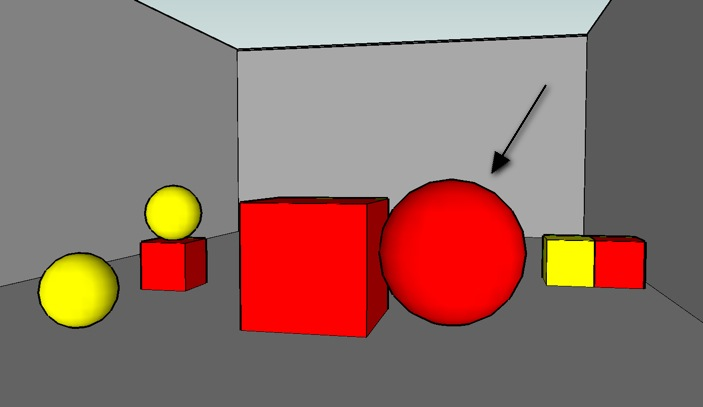
\includegraphics[width=\textwidth]{images/22sinletras.jpg}
%%\caption{Ejemplo de contexto}
%\label{GRE3D7-stimulus1-b}
\vspace*{1cm}
\begin{picture}(250,50)
\put(0,-50){\begin{tikzpicture}
  [
    n/.style={circle,draw,inner sep=1.5pt,node distance=1.5cm},
		 aArrow/.style={->, >=stealth, semithick, shorten <= 1pt, shorten >= 1pt},
  ]
 \node[n,label=below:{
    \relsize{-2}$\begin{array}{c}
      \nSmall\\[-3pt] 
      \nYellow \\[-3pt] 
      \nBall\end{array}$}] (a) {$e_1$};
 \node[n,label=below:{
    \relsize{-2}$\begin{array}{c}     
      \nSmall\\[-3pt] 
      \nRed\\[-3pt] 
      \nCube\end{array}$}, right of=a] (b) {$e_2$};
 \node[n,label=above:{
    \relsize{-2}$\begin{array}{c}     
      \nSmall\\[-3pt] 
      \nYellow\\[-3pt] 
      \nBall\end{array}$}, above of=b] (c) {$e_3$};
 \node[n,label=below:{
    \relsize{-2}$\begin{array}{c}
      \nLarge\\[-3pt] 
      \nRed\\[-3pt] 
      \nCube\end{array}$}, right of=b] (d) {$e_4$};
 \node[n,label=below:{
    \relsize{-2}$\begin{array}{c}
      \nLarge\\[-3pt] 
      \nRed\\[-3pt] 
      \nBall\end{array}$}, right of=d] (e) {$e_5$};
 \node[n,label=below:{
    \relsize{-2}$\begin{array}{c}
      \nSmall\\[-3pt] 
      \nYellow\\[-3pt] 
      \nCube\end{array}$}, right of=e] (f) {$e_6$};
 \node[n,label=below:{
    \relsize{-2}$\begin{array}{c}
      \nSmall\\[-3pt]
      \nRed\\[-3pt] 
      \nCube\end{array}$},  right of=f] (g) {$e_7$};
 \draw [aArrow,bend right=40] (b) to node[auto,swap]{\relsize{-3}$\nBelow$} (c);
 \draw [aArrow,bend right=40] (c) to node[auto,swap]{\relsize{-3}$\nOntop$} (b);
 \draw [aArrow,bend right=40] (d) to node[auto,swap]{\relsize{-3}$\nLeftof$} (e);
 \draw [aArrow,bend right=40] (e) to node[auto,swap]{\relsize{-3}$\nRightof$} (d);
 \draw [aArrow,bend right=40] (f) to node[auto,swap]{\relsize{-3}$\nLeftof$} (g);
 \draw [aArrow,bend right=40] (g) to node[auto,swap]{\relsize{-3}$\nRightof$} (f);
 
 \draw [aArrow,bend right=40] (a) to node[auto,swap]{} (b);
 \draw [aArrow,bend right=40] (b) to node[auto,swap]{} (a);

 \draw [aArrow,bend right=40] (b) to node[auto,swap]{} (d);
 \draw [aArrow,bend right=40] (d) to node[auto,swap]{} (b);

\draw [aArrow,bend right=40] (e) to node[auto,swap]{} (f);
 \draw [aArrow,bend right=40] (f) to node[auto,swap]{} (e);
 %\draw[dotted] (-0.5,-1.3) rectangle (8,3.1);
 \draw[dotted] (-0.5,-1.5) rectangle (8,3);
 \end{tikzpicture}}
 \end{picture}
 %\end{flushleft}

\vspace*{2cm} 
 \caption{Representaci\'on de contexto m\'as completo.}\label{representacion-modelo-completo}
\end{figure}


Aunque no hablemos ni de incompletitud ni de incorrectitud tambi\'en hay incertidumbre en \textbf{cu\'al} de todas las posibles ERs un sistema de GER debe 
elegir. Por ejemplo seguramente hay personas que preferir\'an ERs que usen la palabra \emph{esfera}, antes que \emph{bola}. Y seguramente 
no falte quien diga que \emph{la} mejor expresi\'on referencial ni si quiera aparece en la Figura \ref{figura-er}. Sin embargo, seguramente 
habr\'a una tendencia como se muestra en estudios previos \cite{viet:gene11}. Nadie preferir\'a una ER que use 21 propiedades y 6 relaciones 
para describir al target de la Figura \ref{figura-er}.

El largo de una ER afecta su calidad. Se podr\'{i}a pensar, por ejemplo, que las referencias son \'optimas cuando son \textbf{m\'{i}nimas}
 en longitud, es decir, cuando contienen s\'olo informaci\'on suficiente para identificar el objeto target y nada m\'as. Pero la generaci\'on de referencias m\'{i}nimas
no es lo que las personas hacen ni lo que es m\'as \'util para los oyentes, como se muestra en trabajo previo \cite{Lu_sasha2015}. Y ni si quiera 
nos resuelve el problema de elegir una ER. {\it La bola grande} y {\it La esfera roja} son dos ERs de la Figura \ref{figura-er} y tienen 
exactamente la misma longitud.

Dado que la incertidumbre es inherente a la tarea de GER, lo mejor que se puede hacer es que un algoritmo de GER devuelva un \textbf{ranking}
 de ERs, o lo que es lo mismo, un conjunto de ERs en el que cada ER tiene un valor asociado que intenta reflejar cu\'an buena es esa ER para el input dado.

?`Como podemos generar un ranking de ERs?.
Un algoritmo simplista generar\'ia primero todas las ERs posibles y luego las ordenar\'ia con alg\'un criterio. Esto es posible porque la cantidad de ERs es finita dado un modelo finito, pero esta cantidad puede ser muy grande, exponencial en el tama\~{n}o del modelo y la gran mayor\'ia de estas ERs no se llegar\'ian a usar en una aplicaci\'on real. Una aplicaci\'on s\'olo usar\'a las mejores ERs de un target considerado.
Una forma m\'as eficiente de generar un ranking de ERs es dise\~{n}ar un algoritmo no determin\'istico y correrlo una cantidad de veces suficiente para la aplicaci\'on.

Un algoritmo para la GER es {\bf no-determin\'istico} si puede dar diferentes ERs para el mismo contexto y target en sucesivas ejecuciones. 
Para producir un ranking de las mejores ERs para un target, el no determinismo debe estar guiado de alguna forma que le permita dar m\'as veces ERs m\'as frecuentes, y menos veces las menos frecuentes. Llamaremos a esta gu\'ia: \textbf{probabilidad de uso} de una propiedad o relaci\'on. Esta probabilidad se puede ver afectada por caracter\'isticas de la propiedad o relaci\'on (tipos de propiedades) o por caracter\'isticas de qui\'en interpretar\'a la ER (el interlocutor).

Hay diferentes \textbf{tipos de propiedades}, por ejemplo taxon\'omicas (las que tiene el objeto, como \emph{esfera}, o \emph{roja}), relacionales (las que necesitan dar una expresi\'on de otro objeto, por ejemplo {\it estar al lado de}), vagas (son las m\'as dif\'iciles de identificar, por ejemplo: \emph{chico}, \emph{grande}, no son propiedades absolutas, ya que necesitan un contexto, ?`con respecto a qu\'e algo es chico o grande?). Ciertos valores de propiedades pueden ser m\'as f\'aciles de identificar que otros, por ejemplo cierto color verde podr\'{i}a ser m\'as complicado de identificar que el tama\~no grande de un objeto. Notar que cuando decimos el tama\~no, tenemos como marco de referencia a los objetos de la escena, en ese contexto un objeto es {\it grande}.
%En esta tesis estudiamos la generaci\'on autom\'atica de expresiones referenciales, 
%primero mostramos c\'omo podemos a\~nadir no determinismo a los algoritmos estudiados. Los algoritmos de refinamiento estudiados, tienen un orden fijo en el cual consideran las propiedades y relaciones, y la naturalidad de las expresiones referenciales que generan depende de este orden particular considerado, nosotros proponemos reemplazar ese orden fijo sobre las propiedades y/o relaciones de la escena de entrada por una~\emph{probabilidad de uso} para cada propiedad y/o relaci\'on, y modificar los algoritmos para que tengan en cuenta esas propiedades. De esta manera, cada llamada al algoritmo puede producir diferentes ERs para la misma escena y target de entrada. 

%Es decir nuestra meta, no s\'olo ser\'a crear algoritmos para la generaci\'on autom\'atica de expresiones referenciales, sino crearlos de tal manera que podamos imitar en gran medida lo que dir\'ian las personas.
%
%Mostraremos que dado un corpus (como el corpus GRE3D7 o el TUNA de los cuales hablaremos en Cap\'itulo~\ref{sec:seleccion}) podemos estimar estas probabilidades de uso de manera que las ER se generen con una distribuci\'on de probabilidad que coincide en gran medida con las que se encuentra en el corpus.

Esta selecci\'on de la ER m\'as apropiada tambi\'en debe tener en cuenta al \textbf {interlocutor}, es natural que los humanos demos distintas ERs a distintos interlocutores.
% En el \'area muchas veces se habla de optimalidad de la ER, pero con diferentes significados, para algunos una ER \'optima es aquella que dice lo m\'inimo necesario para identificar al objeto target, para otros es la menos esfuerzo requiere del interlocutor para identificarlo.
La selecci\'on de qu\'e propiedades y/o relaciones con otros objetos incluir en una expresi\'on referencial depender\'a del prop\'osito que tengamos para dicha expresi\'on referencial. Una expresi\'on referencial ser\'a muy distinta si nuestro objetivo es dar la m\'inima informaci\'on que distinga al objeto, que si nuestro objetivo es ayudar al interlocutor a que identifique el objeto.

La generaci\'on de expresiones referenciales en el mundo real sufre de diversas fuentes de incertidumbre. En esta tesis proponemos formas para modelar esta incertidumbre partiendo de t\'ecnicas de representaci\'on de conocimiento basadas en teor\'ia de modelos.
%En la vida real hay muchas cosas que nos ayudan a darnos cuenta si nuestro interlocutor identific\'o el objeto target, como ser la expresi\'on de duda nos dar\'ia una pauta de que no esta entendiendo lo que le queremos decir...
%
%\textbf{FALTA CIERRE A ESTA SECCION!}

%En esta tesis nos vamos a enfocar en la selecci\'on de contenidos de las expresiones referenciales, y el objetivo ser\'ia simular el comportamiento humano, para ello vamos a usar corpus de expresiones referenciales para aprender como realizan esta tarea las personas.
 %
%Las propiedades y relaciones de los objetos de la escena forman una base de conocimento, estos datos se pueden organizar en jerarqu\'ias, por ejemplo: conjunto de animales, conjunto de mamiferos, conjunto de insectos. Algunos conjuntos pueden estar contenidos en otros, es decir algunos objetos o entidades pueden compartir caracter\'isticas.
%
%Si el objeto target tiene la propiedad de medir 1.80 de alto, y est\'a en un grupo donde los dem\'as son m\'as peque\~nos, es m\'as natural decir el m\'as alto, que el que mide 1.80.
%Si tenemos 100 caracter\'isticas de una persona, y con esas caracter\'isticas se pudiera identificar un\'ivocamente a una persona, un sistema que diera que las 100 caracter\'isticas no ser\'ia un sistema que suene muy natural, ya que una persona no dar\'ia 100 propiedades para identificar a una persona particular. As\'i podr\'iamos decir que las expresiones referenciales variaran seg\'un la cantidad de informaci\'on que contienen, si contienen la m\'inima informaci\'on para identificarlas un\'ivocamente ser\'an minimales, si contienen m\'as informaci\'on estar\'an sobreespecificadas, pero en el caso de contener m\'as de la m\'inima informaci\'on para identificarlas un\'ivocamente... cu\'anta m\'as dar?, intentaremos imitar lo que hacen las personas cuando dan expresiones referenciales para responder este tipo de preguntas.
%El sistema deber\'ia tener una lista del orden de preferencia de los atributos a usar.\\ 



%NO NO Las primeras investigaciones en GER no voy a poner esto porque no quiero pasar por alto shrdlu de vinogran 1969
%\cite{C92-1038}; \cite{Dale95computationalinterpretations} hicieron una serie de supuestos simplificadores, por ejemplo no usaban relaciones, el target era un s\'olo objeto, y como resultado los primeros
%algoritmos GER s\'olo pod\'ian generar una variedad limitada de expresiones referenciales. Cuando
%los investigadores comenzaron a levantar algunos de estos supuestos, esto di\'o lugar a algoritmos de GER
%con un repertorio m\'as amplio, siendo capaces de generar, por ejemplo, plurales y expresiones relacionales. 
%
%Este movimiento ha creado una serie de nuevos desaf\'ios, sin embargo. Por ejemplo, el
%n\'umero de formas en las que uno puede referirse a un conjunto de objetos de destino aumenta, por lo que la elecci\'on de una
%buena expresi\'on referencial es m\'as dif\'icil.
%
%Del mismo modo, incluso propuestas recientes tienden a asumir que no es problem\'atico para determinar qu\'e informaci\'on
%es compartida entre el hablante y el oyente.\\
%(a) C\'omo se representa la informaci\'on del dominio?\\
%(b) C\'omo se representa el contenido sem\'antico de una expresi\'on referencial? \\
%(c) C\'omo se pueden encontrar descripciones distintivas?
%
%En los contextos de los corpus analizados en esta tesis, nos encontramos con cuatro tipos diferentes de atributos:
%tipos de objetos, atributos absolutos, atributos relativos, atributos espaciales incluidas las relaciones y atributos de localizaci\'on.
%
%El tipo de un objeto constituye un caso especial, ya que es muy rara vez omite
%en la expresi\'on referencial. En consecuencia, la mayor\'ia de los algoritmos tratan de
%considerarlo por separado para asegurarse de que se a\~nade a cada expresi\'on referencial. Una explicaci\'on parcial para esta condici\'on especial es que las expresiones referenciales se realizan como sintagmas nominales,
%cada sintagma nominal requiere un sustantivo, y por lo general es el tipo del referente dado que es el sustantivo principal.
%
%\section{Contribuciones de esta tesis}
%\label{sec:contribiciones}
%\textcolor{blue}{Esta parte se va?}
%\begin{itemize}
%\item Se estudi\'o el avance en el \'area de la generaci\'on autom\'atica de expresiones referenciales, los algoritmos existentes y los problemas que ellos ten\'ian, las aproximaciones emp\'iricas realizadas en el \'area en el Cap\'itulo~\ref{sec:seleccion}.
%\item Se estudiaron las m\'etricas de evaluaci\'on tanto autom\'aticas como manuales en el Cap\'itulo~\ref{sec:seleccion}, las cuales ser\'an luego aplicadas en el Cap\'itulo~\ref{sec:evaluacion}.
%%\item Se abordaron los siguientes problemas: no-determinismo, sobreespecificaci\'on.
%\item Se estudiaron estudiaron distintas l\'ogicas y sus lenguajes asociados, se compararon esos lenguajes con el lenguaje utilizado para dar ER, a fin de elegir una l\'ogica apropiada en el Cap\'itulo~\ref{sec:intro_logica}.
%\item Se seleccion\'o un algoritmo existente al cual se le agregaron probabilidades de uso para simular el no-determinismo encontrado en corpus. Este fue seleccionado por permitirmos agregar los aspectos tenidos en cuenta en esta tesis: dar un algoritmo que aborde el no-determinismo, la sobreespecificaci\'on que sea relacional, que genere plurales en el Cap\'itulo~\ref{sec:learning}.
%%\item Se modific\'o el algoritmo para que sea no-determinista.
%\item Se agreg\'o sobreespecificaci\'on al algoritmo permitiendo agregar propiedades o relaciones cuando estas tienen una alta probabilidad de uso en corpus. Y al mismo tiempo se agura la terminaci\'on en el Cap\'itulo~\ref{sec:algoritmo}.
%\item Se propone un m\'etodo para calcular las probabilidades de uso (\puse)\ de las relaciones del modelo el cual genera una distribuci\'on de expresiones referenciales cercana a la encontrada en el corpus.
%\item Se prob\'o el algoritmo en 2 corpus existentes (el GRE3D7 y el Tuna corpus) en el Cap\'itulo~\ref{sec:evaluacion}.
%\item Se realiz\'o una evaluaci\'on en la que se compararon las salidas del algoritmo con ambos corpus. Se usaron m\'etricas autom\'aticas y manuales Cap\'itulo~\ref{sec:evaluacion}.
%\item Se creo un corpus de descripciones de mapas (el ZOOM corpus).
%\item Se hizo un caso de estudio de 3 mapas del ZOOM corpus explicado en Cap\'itulo~\ref{sec:corpus}, en el cual se toma 1 mapa con target singular, el mismo mapa con zoom 2x y target singular y el mismo mapa con target plural.
%\end{itemize}



\section{Expresiones referenciales usando teor\'ia de modelos}
\label{sec:gre-teoria-modelos}

Los \textbf{modelos relacionales} tambi\'en conocidos como \textbf{modelos de kripke} y \textbf{modelos de primer orden} son muy utilizados para la representaci\'on de situaciones o escenas. 
Los modelos relacionales son grafos etiquetados y pueden verse tambi\'en como aut\'omatas finitos. Estas estructuras matem\'aticas han sido muy estudiadas y tienen muchas propiedades bien conocidas \cite{arec:hybr05b}. En esta tesis se adaptan algoritmos cl\'asicos de minimizaci\'on de aut\'omatas aplicados a la caracterizaci\'on de modelos relacionales.

Para un \textbf{vocabulario} de s\'imbolos relacionales r, un modelo relacional $\+M$ es una tupla $\tup{\Delta,\interp{\cdot}}$ donde:
\begin{itemize}
 \item $\Delta$ es un conjunto no vac\'io de objetos ---el dominio---
 \item $\interp{\cdot}$ es una funci\'on de interpretaci\'on, esto es, $\interp{r} \subseteq \Delta^n$ para todo s\'imbolo de relaci\'on $n$-ario $r$ que est\'a en el vocabulario.  
\end{itemize}
El \emph{tama\~no} de un modelo $\+M$ es la suma ($\#\Delta + \#\interp{\cdot}$), donde $\#\Delta$ es la cardinalidad
de $\Delta$ y $\#\interp{\cdot}$ es la suma de todas las aridades de las relaciones en $\interp{\cdot}$.
Si asumimos un vocabulario finito de s\'imbolos de relaci\'on $n$-arios entonces $\+M$ es \emph{finito}. 


%Un modelo relacional $\+M$ es una tupla 
%$\tup{\Delta,\interp{\cdot}}$ donde $\Delta$ es un conjunto no vac\'io, y
%$\interp{\cdot}$ es una funci\'on de interpretaci\'on, esto es,
%$\interp{r} \subseteq \Delta^n$ para todo s\'imbolo de relaci\'on $n$-aria tal que
%$r$ est\'a en el vocabulario. $\+M$ es \emph{finito} cuando
%$\Delta$ es finito.  El \emph{tama\~no} de un modelo $\+M$ es la suma
%$\#\Delta + \#\interp{\cdot}$, donde $\#\Delta$ es la cardinalidad
%de $\Delta$ y $\#\interp{\cdot}$ es la suma de todas las aridades de las
%relaciones en $\interp{\cdot}$.

A continuaci\'on vamos a presentar 2 ejemplos de modelos relacionales, uno en el que tenemos entidades \textbf{agentivas} (es decir, agentes animados que pueden realizar acciones) como perros y gatos, y otro en el que las entidades son \textbf{no agentivas}, es decir, son objetos est\'aticos.

El primer ejemplo se muestra en la Figura~\ref{fig:cat-dog-1} en la cual hemos representado un contexto
como un modelo relacional. Intuitivamente, $a$, $b$ y $d$ son perros, mientras que 
$c$ y $e$ son gatos;  $d$ es un peque\~no beagle; $b$ y $c$ tambi\'en son peque\~nos.
 Leeremos $\aSniffing(d,e)$ como ``{\em $d$ huele a $e$}''. La interpretaci\'on del s\'imbolo relacional $\nDog$ es $\interp{\nDog}$  =  $\cset{a,b,d}$ ya que $a$, $b$ y $d$ son los \'unicos perros del contexto. La interpretaci\'on de $\aSniffing$ es el conjunto de pares de elementos que cumplen $\aSniffing$. Por ejemplo ($a,a$) pertenece al conjunto dado que $a$ es un perro que se huele a s\'i mismo en el modelo.

 \begin{figure}[!ht]
 %\begin{center}
 \begin{tabular}{rcl}
$\Delta$               & = & $\cset{a,b,c,d,e}$\\
$\interp{\nDog}$      & = & $\cset{a,b,d}$\\
$\interp{\nCat}$      & = & $\cset{c,e}$\\
$\interp{\nBreed}$    & = & $\cset{d}$\\
$\interp{\aSmall}$    & = & $\cset{b,c,d}$\\
$\interp{\aSniffing}$ & = & $\cset{(a,a),(b,a),(c,b),(d,e),(e,d)}$
 \end{tabular}
\begin{picture}(90,30)
\put(0,-40){\begin{tikzpicture}
  [
    n/.style={circle,draw,inner sep=1.5pt,node distance=1.5cm},
    aSniffing/.style={->, >=stealth, semithick, shorten <= 3pt, shorten >= 3pt},
  ]
 \node[n,label=below:{\relsize{-1}$\begin{array}{c}\nDog\end{array}$}] (a) {$a$};

 \node[n,label=below:{\relsize{-1}$\begin{array}{c}\nDog\\ \aSmall \end{array}$}, right of=a] (b) {$b$};

 \node[n,label=below:{\relsize{-1}$\begin{array}{c}\nCat\\ \aSmall\end{array}$}, right of=b] (c) {$c$};

 \node[n,label=below:{\relsize{-1}$\begin{array}{c}\nDog\\ \nBreed\\  \aSmall \end{array}$}, right of=c] (d) {$d$};

 \node[n,label=below:{\relsize{-1}$\begin{array}{c}\nCat\end{array}$},right of=d] (e) {$e$};

 \draw [aSniffing,loop left] (a) to node[above,xshift=-5pt]{\relsize{-1}$\aSniffing$} (a);

 \draw [aSniffing,bend right=40] (b) to node[auto,swap]{\relsize{-1}$\aSniffing$} (a);

 \draw [aSniffing,bend right=40] (c) to node[auto,swap]{\relsize{-1}$\aSniffing$} (b);

 \draw[aSniffing, bend left=40] (d) to node[auto]{\relsize{-1}$\aSniffing$} (e);
 \draw[aSniffing, bend left=40] (e) to node[auto,swap]{\relsize{-1}$\aSniffing$} (d);

 \end{tikzpicture}}
 \end{picture}

 %\end{center}
 \caption{Representaci\'on de escena como un modelo relacional e interpretaci\'on de sus propiedades y relaciones. Ejemplo con entidades agentivas.\label{fig:cat-dog-1}}
 \end{figure}

El segundo ejemplo se muestra en la Figura~\ref{grafo-GRE3D7-stimulus_b} donde damos una posible representaci\'on de la escena de la Figura \ref{figura-er} como un modelo relacional. El dominio es $\Delta$  = $\cset{e_1,e_2,e_3,e_4,e_5,e_6,e_7}$. La interpretaci\'on de $\nBall$ es $e_1$, $e_3$ y $e_5$, ya que estos objetos son esferas, la de $\nCube$ es $\interp{\nCube}$ =$\cset{e_2, e_4, e_6, e_7}$, ya que esos objetos son cubos. Tenemos las relaciones $\nRightof$, $\nLeftof$, $\nBelow$ y $\nOntop$, cuyas interpretaciones se muestran en la figura. Como discutimos en la secci\'on anterior, se puede argumentar que este modelo est\'a incompleto, pero es suficiente para los objetivos ilustrativos de esta secci\'on.

\begin{figure}
\begin{flushleft}
\begin{tabular}{rcl}
$\Delta$              & = & $\cset{e_1,e_2,e_3,e_4,e_5,e_6,e_7}$\\
$\interp{\aRed}$      & = & $\cset{e_2,e_4,e_5,e_7}$\\
$\interp{\aYellow}$   & = & $\cset{e_1,e_3,e_6}$\\
$\interp{\nBall}$     & = & $\cset{e_1,e_3,e_6}$\\
$\interp{\nCube}$     & = & $\cset{e_2,e_4,e_6,e_7}$\\

$\interp{\aSmall}$    & = & $\cset{e_1,e_2,e_3,e_6,e_7}$\\
$\interp{\aLarge}$    & = & $\cset{e_4,e_5}$\\

$\interp{\nRightof}$   & = & $\cset{(e_4,e_5),(e_6,e_7)}$\\
$\interp{\nLeftof}$    & = & $\cset{(e_5,e_4),(e_7,e_6)}$\\
$\interp{\nOntop}$     & = & $\cset{(e_3,e_2)}$\\
$\interp{\nBelow}$     & = & $\cset{(e_2,e_3)}$\\

 \end{tabular}
\begin{picture}(120,50)
\put(0,-50){\begin{tikzpicture}
  [
    n/.style={circle,draw,inner sep=1.5pt,node distance=1.5cm},
		 aArrow/.style={->, >=stealth, semithick, shorten <= 1pt, shorten >= 1pt},
    %aSniffing/.style={->, >=stealth, semithick, shorten <= 3pt, shorten >= 3pt},
  ]
%\begin{tikzpicture}
%  [
%    n/.style={circle,fill,draw,inner sep=3pt,node distance=2cm},
%    aArrow/.style={->, >=stealth, semithick, shorten <= 1pt, shorten >= 1pt},
%  ]
 \node[n,label=below:{
    \relsize{-2}$\begin{array}{c}
      \nSmall\\[-3pt] 
      \nYellow \\[-3pt] 
      \nBall\end{array}$}] (a) {$e_1$};
 \node[n,label=below:{
    \relsize{-2}$\begin{array}{c}     
      \nSmall\\[-3pt] 
      \nRed\\[-3pt] 
      \nCube\end{array}$}, right of=a] (b) {$e_2$};
 \node[n,,label=above:{
    \relsize{-2}$\begin{array}{c}
      \nSmall\\[-3pt] 
      \nYellow\\[-3pt] 
      \nBall\end{array}$}, above of=b] (c) {$e_3$};
 \node[n,label=below:{
    \relsize{-2}$\begin{array}{c}
      \nLarge\\[-3pt] 
      \nRed\\[-3pt] 
      \nCube\end{array}$}, right of=b] (d) {$e_4$};
 \node[n,label=below:{
    \relsize{-2}$\begin{array}{c}
      \nLarge\\[-3pt] 
      \nRed\\[-3pt] 
      \nBall\end{array}$}, right of=d] (e) {$e_5$};
 \node[n,,label=below:{
    \relsize{-2}$\begin{array}{c}
      \nSmall\\[-3pt] 
      \nYellow\\[-3pt] 
      \nCube\end{array}$}, right of=e] (f) {$e_6$};
 \node[n,label=below:{
    \relsize{-2}$\begin{array}{c}
      \nSmall\\[-3pt]
      \nRed\\[-3pt] 
      \nCube\end{array}$},  right of=f] (g) {$e_7$};
 \draw [aArrow,bend right=40] (b) to node[auto,swap]{\relsize{-3}$\nBelow$} (c);
 \draw [aArrow,bend right=40] (c) to node[auto,swap]{\relsize{-3}$\nOntop$} (b);
 \draw [aArrow,bend right=40] (d) to node[auto,swap]{\relsize{-3}$\nLeftof$} (e);
 \draw [aArrow,bend right=40] (e) to node[auto,swap]{\relsize{-3}$\nRightof$} (d);
 \draw [aArrow,bend right=40] (f) to node[auto,swap]{\relsize{-3}$\nLeftof$} (g);
 \draw [aArrow,bend right=40] (g) to node[auto,swap]{\relsize{-3}$\nRightof$} (f);
 
%\draw[dotted] (-0.5,-1.3) rectangle (8,3.1);

% \end{tikzpicture}
%\caption{Grafo del contexto \ref{GRE3D7-stimulus}}
%\label{grafo-GRE3D7-stimulus_b}
%\end{figure}
 \end{tikzpicture}}
 \end{picture}
 \end{flushleft}
 \caption{Representaci\'on de la escena de la Figura \ref{figura-er} como un modelo relacional e interpretaci\'on de sus propiedades y relaciones. Ejemplo con entidades no agentivas.}
 \label{grafo-GRE3D7-stimulus_b}
 \end{figure}

Ahora nos enfocaremos en conseguir ERs para identificar a targets dados usando los modelos que acabamos de describir. Veremos lenguajes de distintas l\'ogicas y c\'omo las f\'ormulas l\'ogicas pueden representar a las ERs.
%Los lenguajes l\'ogicos son \'utiles para la tarea de describir (formalmente) elementos de una estructura relacional. 
A continuaci\'on definimos el lenguaje cl\'asico de la l\'ogica de primer orden (con desigualdad), \FOL. Dicho lenguaje se define inductivamente como sigue. Una f\'ormula $\phi$ es una f\'ormula de \FOL si es de alguna de las siguientes formas:

% *2 est\'a dado por $\top$ que es como decir 'cosa', todo elemento satisface $\top$, la desigualdad entre 2 elementos $ x_i$ y $x_j$, relaciones de tuplas, la negaci\'on de f\'ormulas de \FOL, la conjunci\'on de f\'ormulas de \FOL, y el existencial de una variable ligada en la f\'ormula de \FOL:
\begin{enumerate}
  \item $\top$ Es como decir {\it cosa}, todo elemento satisface $\top$.
  \item $x_i \not\approx x_j$ La desigualdad entre dos elementos $x_i$ y $x_j$.
  \item $r (\bar x)$ Relaciones de tuplas.
  \item $\lnot \gamma$ Negaci\'on de f\'ormulas.
  \item $\gamma \land \gamma'$ Conjunci\'on de f\'ormulas.
  \item $\exists x_i . \gamma$ Existencial de una variable ligada en la f\'ormula $\gamma$.
\end{enumerate}
%
donde $\gamma,\gamma' \in \FOL$,
$r$ es un s\'imbolo de relaci\'on $n$-aria y $\bar x$ es una tupla de $n$ variables.
Como es usual, $\gamma \lor \gamma'$ y $\forall x . \gamma$ son las versiones cortas de
$\lnot(\lnot\gamma \land \lnot\gamma')$ y $\lnot\exists x . \lnot\gamma$, respectivamente.
F\'ormulas de la forma $\top$, $x_i \not\approx x_j$ y $r(\bar
x)$ son llamados \emph{\'atomos}.%

Dado un modelo relacional $\+M = \tup{\Delta,\interp{\cdot}}$ y una
f\'ormula $\gamma$ con variables libres%
\footnote{%
    Asumimos que cada variable no puede aparecer libre y ligada a la vez, que una variable no est\'a ligada 2 veces,
    y que el \'indice de las variables crece en la f\'ormula de izquierda a derecha.%
}
$x_1\ldots x_n$, inductivamente definimos la \textbf{extensi\'on} o
\textbf{interpretaci\'on} de $\gamma$ como el conjunto de $n$-tuplas
 $\interp{\gamma}^n \subseteq \Delta^n$ que satisface:

\begin{enumerate}

\item $\interp{\top}^n$ $=$ $\Delta^n$

\item $\interp{x_i \not\approx x_j}^n$ $=$ $\cset{\bar{a} \mid \bar{a} \,{\in}\, \Delta^n, a_i \neq a_j}$

\item $\interp{\lnot\delta}^n$ $=$ $\Delta^n \setminus \interp{\delta}^n$

\item $\interp{r (x_{i_1} \ldots x_{i_k})}^n$ $=$ $\cset{\bar{a} \mid \bar{a} \,{\in}\, \Delta^n, (a_{i_1} \ldots a_{i_k}) {\in} \interp{r}}$

\item $\interp{\delta \land \theta}^n$ $=$ $\interp{\delta}^n \cap \interp{\theta}^n$

\item $\interp{\exists x_{l}.\delta}^n$ $=$ $\cset{\bar a \mid \bar a  e  \in \interp{\delta'}^{n+1}\ \text{para alg\'un elemento $e$}}$

\end{enumerate}

donde $1 \le i,j, i_1, \ldots, i_k \le n$, $\bar{a} = (a_1\ldots
a_n)$, $\bar{a}e = (a_1\ldots a_n,e)$ y $\delta'$ son
obtenidos reeplazando todas las ocurrencias de $x_l$ en $\delta$ por
$x_{n+1}$. 
%Cuando la cardinalidad de las tuplas involucradas en el contexto es conocida 
%escribiremos $\interp{\phi}$ en lugar de
%$\interp{\phi}^n$.

Con una sintaxis y sem\'antica de un lenguaje en mente, podemos formalmente definir el problema de \textbf{GER en $\gL$} ($\gL$-GER) para un conjunto target de elementos $T$. $\gL$ es el lenguaje de la l\'ogica elegida, en este caso hemos explicado la l\'ogica de primer orden $\FOL$, y en el Cap\'itulo \ref{sec:intro_logica} restringiremos esa l\'ogica para obtener ERs m\'as cercanas a las que aparecen en corpora y para conseguir algoritmos computacionalmente m\'as eficientes.

\medskip
\noindent
{\small
\begin{center}
\begin{tabular}{ll} \hline
\multicolumn{2}{l}{
\textsc{Problema $\gL$-GER }}\\ \hline
\ \ Entrada: & un modelo $\gM=\tup{\Delta,\interp{\cdot}}$ y un conjunto target no vac\'io $T \subseteq \Delta$.\\
\ \ Salida: & una f\'ormula $\varphi \in \gL$ tal que
$\interp{\varphi} = T$ si existe, y $\bot$ caso contrario.\\ \hline
\end{tabular}
\end{center}}

La salida del problema $\+L$-GER es una f\'ormula de
$\+L$ cuya interpretaci\'on en el modelo de input $\gM$ es el conjunto target $T$, si
esa f\'ormula existe. 
Cuando la salida no es $\bot$, decimos que $\phi$ es una
\textbf{expresi\'on referencial en $\+L$ (ER-$\+L$)} para $T$ en $\+M$, y cuando es $\bot$ puede ser que la l\'ogica elegida no sea lo suficientemente expresiva para identificar al target, o que el modelo dado no tenga suficiente detalle.

Consideramos s\'olo modelos relacionales con s\'imbolos de relaciones unarias y binarias, usaremos $p$ para las proposiciones (propiedades) y $r$ para los s\'imbolos de relaci\'on binarias.
Como dijimos anteriormente, dado un modelo $\gM$, podr\'ia haber un n\'umero muy grande de f\'ormulas que de forma un\'ivoca
describan al target (incluso f\'ormulas que no son l\'ogicamente equivalentes podr\'ian tener
la misma interpretaci\'on una vez que el modelo este fijo). Por ejemplo, en el modelo $\+M$ de la Figura \ref{grafo-GRE3D7-stimulus_b} las f\'ormulas $\aLarge \land \nBall$ y $\aRed \land \nBall$ no son l\'ogicamente equivalentes pero tienen la misma interpretaci\'on en $\gM$ ya que $\interp{\aLarge \land \nBall}$ = \{$e_5$\} y $\interp{\aRed \land \nBall}$ = \{$e_5$\}.
Diferentes ERs
del mismo target podr\'ian ser m\'as o menos apropiadas en el contexto dado. Otra cosa que es importante tener en cuenta, es que la determinaci\'on de contenido usando lenguajes con diferente poder expresivo, puede tener un impacto en la complejidad computacional de la GER y en la etapa posterior de realizaci\'on sint\'actica. Para ilustrar eso, veamos las f\'ormulas que identifican al elemento target $b$ en la Figura \ref{fig:cat-dog-1}.

\begin{figure}[h]
$$
\begin{array}{ll}
 \phi_1:  \nDog(x) \land \aSmall(x) \land
   \exists y . (\aSniffing(x,y) \land \nDog(y))\\
  %
  \phi_2:  \nDog(x) \land \aSmall(x) \land
  \forall y . (\neg \nCat(y) \lor \neg \aSniffing(x,y))\\
  %
  \phi_3:  \nDog(x) \land
  \exists y . (x \not\approx y \land \nDog(y)  \land \aSniffing(x,y))\\
  %
  \phi_4:  \nDog(x) \land
  \exists y . (\nCat(y) \land \aSmall(y) \land \aSniffing(y,x))
  %
 \end{array}
$$
\caption{Descripciones alternativas para el objeto $b$ del modelo mostrado en Figura~\protect\ref{fig:cat-dog-1}.}\label{tab:gammas}
\end{figure}

Notar que las f\'ormulas mostradas, hacen uso de diferentes operadores de la l\'ogica \FOL: hay negaci\'on de \'atomos y de relaciones, hay cuantificaci\'on existencial, y universal, conjunci\'on, disyunci\'on y desigualdad. La realizaci\'on sint\'actica de algunas de \'estas f\'ormulas pueden involucrar estructuras gramaticales complejas como voz pasiva como por ejemplo la f\'ormula $\phi_4$ podr\'ia realizarse como {\it El perro que es olido por un gato peque\~no}, verbos reflexivos como en la f\'ormula $\nDog(x) \land \exists y . (x \approx y \land \nDog(y) \land \aSniffing(x,y))$ que representa al target $a$ de la Figura \ref{fig:cat-dog-1} y puede realizarse como {\it El perro que se huele a si mismo}, negaciones, etc. Hay lexemas dif\'iciles de caracterizar sem\'anticamente (como s\'olo) por ejemplo en la f\'ormula $\phi_2$, que podr\'ia realizarse como {\it El perro que huele s\'olo perros que no son el mismo}.
 
%por ejemplo $\phi_2$ podr\'a realizarse como {\it Small dog that sniffs only dogs}. $\phi_3$ podr\'ia realizarse como {\it Dog that sniffs dogs that are not him self}, $\phi_4$ como {\it The dog that is sniffed by a small cat}.
Como nuestra meta es hacer un ranking de las mejores expresiones referenciales, una manera de acercarnos a esa meta es restringiendo la l\'ogica. Si restringimos a \EPFOL, aseguramos que f\'ormulas como $\phi_2$ no se generar\'an. Si sacaramos el operador distinto ($\not\approx$) del lenguaje, $\phi_3$ tambi\'en queda excluida.
%El hecho de que el lenguaje de representaci\'on utilizado tiene un impacto sobre la determinaci\'on de contenido es obvio, pero no ha recibido la atenci\'on que merece. 
%Areces et al. [1] usaron diferentes l\'ogicas de descripci\'on (una familia de lenguajes formales utilizado en representaci\'on del conocimiento, vea [2]) para clasificar y dar un marco formal para trabajo previo sobre GRE. 
A continuaci\'on presentamos fragmentos de $\FOL$ conocidos como l\'ogicas para la descripci\'on. Por ejemplo, el lenguaje de la l\'ogica para la descripci\'on $\ALC$, se define sint\'acticamente como el conjunto de f\'ormulas que se pueden generar con alguna de las siguientes:
$$
\top \mid p \mid \neg \phi \mid \phi \wedge \phi' \mid  \exists r. \phi
$$
donde $p$ es un s\'imbolo proposicional, $r$ es un s\'imbolo relacional binario, y $\phi$, $\phi'$ son f\'ormulas de $\ALC$.

 Mediante la restricci\'on a f\'ormulas de $\ALC$ 
evitar\'iamos f\'ormulas como $\phi_3$ (es decir con desigualdad). Tambi\'en evitar\'iamos f\'omulas como $\phi_4$ que puede realizarse como {\it El perro que es olido por un peque\~no gato} en el cual tenemos que realizar la parte del existencial como una voz pasiva al aparecer la variable cuantificada $x$ en segundo lugar.

%(siempre aparece cuantificado el elemento en la segunda posici\'on de argumento).
Cada lenguaje l\'ogico puede ser visto como un compromiso entre la expresividad, realizabilidad y complejidad computacional. Para la tarea de GER el uso de un lenguaje u otro debe depender del contexto particular considerado y del target a describir.

Para el segundo ejemplo, supongamos que queremos identificar al objeto $e_5$ de la Figura \ref{grafo-GRE3D7-stimulus_b}. Algunas f\'ormulas posibles
 que identifican un\'ivocamente a $e_5$ en el modelo se muestran en la Figura \ref{tab:phis}.

\begin{figure}[h]
$$
\begin{array}{ll}
 \phi_1: & \aRed(x) \land \nBall(x)\\[3pt]
  %
 \phi_2: & \aLarge(x) \land \nBall(x)\\[3pt]
  %
 \phi_3: & \nLarge(x) \land \aRed(x) \land \nBall(x)\\[3pt]
  %
 \phi_4: & \nLarge(x) \land \aRed(x) \land \nBall(x) \land
   \exists y . (\nRightof(x,y) \land \aLarge(y) \land \aRed(y) \land \nCube(y))\\[3pt]
  %ex1
 \phi_5: & \nLarge(x) \land \aRed(x) \land \nBall(x) \land
  \forall y . (\neg \nBall(y) \lor \neg \nRightof(x,y))\\[3pt]
  %ex 2
 \phi_6: & \nLarge(x) \land \aRed(x) \land \nBall(x) \land
  \exists y . (x \not\approx y \land \nCube(y) \land \nRightof(x,y))\\[3pt]
  %ex 3
 \phi_7: & \nLarge(x) \land \aRed(x) \land \nBall(x) \land
  \exists y . (\nCube(y) \land \aRed(y) \land \nLeftof(y,x))
  %ex 4
 \end{array}
$$
\caption{F\'ormulas alternativas para el objeto $e_5$ de la Figura~\protect\ref{grafo-GRE3D7-stimulus_b}, con lenguaje de $\FOL$.}\label{tab:phis}
\end{figure}

En la Figura \ref{tab:realizaciones-phis}, se muestran algunas realizaciones posibles de las f\'ormulas mostradas en la Figura \ref{tab:phis}, grafos de subf\'ormulas se muestran en la Figura \ref{grafos-formulas}, el de la izquierda pertenece a la f\'ormula $\phi_1$ y el de la derecha a la f\'ormula $\phi_4$.

 \begin{figure}[h]
 %\begin{center}
\hspace*{1.5cm} 
\begin{picture}(0,60)
\put(80,0){\begin{tikzpicture}
  [
    n/.style={circle,draw,inner sep=1.5pt,node distance=1.5cm},
		 aArrow/.style={->, >=stealth, semithick, shorten <= 1pt, shorten >= 1pt},
  ]
 \node[n,label=below:{
    \relsize{-2}$\begin{array}{c}
      \nRed\\[-3pt] 
      \nBall\end{array}$}, right of=d] (e) {$e_5$};
 \end{tikzpicture}}
\end{picture}
\begin{picture}(0,100)
%\hspace*{3.5cm} 
%\vspace*{5.5cm} 

\put(180,0){\begin{tikzpicture}
   [
    n/.style={circle,draw,inner sep=1.5pt,node distance=1.5cm},
		 aArrow/.style={->, >=stealth, semithick, shorten <= 1pt, shorten >= 1pt},
  ]
 \node[n,label=below:{
    \relsize{-2}$\begin{array}{c}
      \nLarge\\[-3pt] 
		  \nRed\\[-3pt] 
      \nCube\end{array}$}, right of=b] (d) {$e_4$};
 \node[n,label=below:{
    \relsize{-2}$\begin{array}{c}
      \nLarge\\[-3pt]
      \nRed\\[-3pt] 
      \nBall\end{array}$}, right of=d] (e) {$e_5$};
 \draw [aArrow,bend right=40] (e) to node[auto,swap]{\relsize{-3}$\nRightof$} (d);
 \end{tikzpicture}}
 \end{picture}
%\end{subfigure}
\caption{Subgrafos que representan las f\'ormulas $\phi_1$ y $\phi_4$.}\label{grafos-formulas}
\end{figure}

%\begin{figure}%{.6\textwidth}
 %\centering
%\begin{subfigure}{.5\textwidth}
%\put(5,-50){
%\begin{tikzpicture}
  %[
    %n/.style={circle,draw,inner sep=1.5pt,node distance=1.5cm},
		 %aArrow/.style={->, >=stealth, semithick, shorten <= 1pt, shorten >= 1pt},
  %]
 %\node[n,label=below:{
    %\relsize{-2}$\begin{array}{c}
      %\nRed\\[-3pt] 
      %\nBall\end{array}$}, right of=d] (e) {$e_5$};
 %\end{tikzpicture}}
 %
%%\vspace*{1.5cm} 
 %\caption{Subgrafo $\nBall \land \nRed$} \label{formula-subgrafo}
%%\vspace*{-1cm}
%\end{subfigure}
%\begin{subfigure}{.5\textwidth}
%
%\put(20,-50){\begin{tikzpicture}
  %[
    %n/.style={circle,draw,inner sep=1.5pt,node distance=1.5cm},
		 %aArrow/.style={->, >=stealth, semithick, shorten <= 1pt, shorten >= 1pt},
  %]
 %\node[n,label=below:{
    %\relsize{-2}$\begin{array}{c}
      %\nRed\\[-3pt] 
      %\nCube\end{array}$}, right of=b] (d) {$e_4$};
 %\node[n,label=below:{
    %\relsize{-2}$\begin{array}{c}
      %\nRed\\[-3pt] 
      %\nBall\end{array}$}, right of=d] (e) {$e_5$};
 %\draw [aArrow,bend right=40] (e) to node[auto,swap]{\relsize{-3}$\nRightof$} (d);
 %\end{tikzpicture}}
%\end{subfigure}
%\vspace*{-2cm} 
 %\caption{Subgrafo $\nBall \land \nRed \land \exists \nRightof . (\nCube  \land \nRed)$} \label{formula-subgrafo2}
%\vspace*{0.5cm}
%\vspace*{1cm}
%\end{figure}%



\begin{figure}[h]

\begin{tabular}{l}
 $\phi_1$: {\it La esfera roja}\\[1pt]
  %
 $\phi_2$: {\it La esfera grande}\\[1pt]
  %
 $\phi_3$: {\it La esfera grande y roja}\\[1pt]
  %
 $\phi_4$: {\it La esfera grande y roja que est\'a a la derecha de un cubo grande y rojo}\\[1pt]
  %ex1
 $\phi_5$: {\it La esfera grande y roja, que no tiene ninguna esfera a la derecha}\\[1pt]
  %ex 2
 $\phi_6$: {\it La esfera grande y roja que est\'a a la derecha de un cubo}\\[1pt]
 % (x \not\approx y \land \nCube(y) \land \nRightof(x,y))
  %ex 3
 $\phi_7$: {\it La esfera grande y roja que tiene un cubo rojo a la izquierda}\\[1pt]
  %ex 4
\end{tabular}
%%$$
\caption{Posibles realizaciones de las f\'ormulas dadas en la Figura \protect\ref{tab:phis}.}\label{tab:realizaciones-phis}
\end{figure}

Notar que $\phi_1$ y $\phi_2$ son m\'inimas, es decir no se puede dar una f\'ormula m\'as corta que esas que identifique al target.
La f\'ormula $\phi_1$, $\phi_2$, $\phi_3$ y $\phi_4$ son caracterizadas como f\'ormulas positivas, conjuntivas y existenciales (no contienen negaci\'on y s\'olo tienen conjunciones y cuantificadores existenciales), este tipo de f\'ormulas son las que m\'as se encuentran en corpora de ERs~\cite{viethen06:_algor_for_gener_refer_expres,deemter06:_build_seman_trans_corpus_for,gre3d3}. Bueno, pero entonces como dijimos reci\'en podemos elegir otra l\'ogica cuyo lenguaje est\'e restringido a las ERs que queremos generar. Restringiendo la determinaci\'on de contenido a \EPFOL, aseguramos que f\'ormulas como  $\phi_5$ no se generar\'an. Si prohibimos el distinto del lenguaje $\phi_6$ tambi\'en queda excluida. La l\'ogica de menor complejidad computacional que se corresponde con todas esas restricciones es \EL. 

En el Cap\'itulo \ref{sec:intro_logica} describimos c\'omo los operadores l\'ogicos afectan la expresividad y la complejidad computacional de la tarea de GER, as\'i como el ranking de ERs generadas. En el Cap\'itulo \ref{sec:algoritmo} proponemos como dicho ranking puede ser mejorado agregando una distribuci\'on finita de probabilidades asociada a los s\'imbolos de relaci\'on del modelo.



\section{Mapa de la tesis}
\label{sec:mapadetesis}

En esta secci\'on contamos como est\'a organizada la tesis. En lo que sigue daremos el resumen de la tem\'atica de cada cap\'itulo.

\subsection{Cap\'itulo~\ref{sec:intro}: ``Introducci\'on''} 
Situamos a la generaci\'on autom\'atica de expresiones 
referenciales dentro de la inteligencia artificial y de la generaci\'on de lenguaje natural. Dijimos que un sistema de 
generaci\'on de lenguaje natural tiene tres etapas: la determinaci\'on de contenido, la lexicalizaci\'on y la realizaci\'on sint\'actica. La generaci\'on de expresiones referenciales es una sub\'area de la generaci\'on de lenguaje natural y por lo tanto, incluye las mismas tres etapas. La determinaci\'on de contenido, que es la selecci\'on de las propiedades y/o relaciones con otros objetos que vamos a elegir para identificar un\'ivocamente al objeto de los dem\'as objetos del contexto, sobre este tema, trabajaremos profundamente en el resto de la tesis. Dimos intuiciones de qu\'e es una expresi\'on referencial en el contexto de una imagen que presentamos. Despu\'es explicamos la importancia de la generaci\'on de expresiones referenciales dentro de la generaci\'on de lenguaje natural, en 
dominios diferentes que van desde generaci\'on de pron\'osticos del tiempo, resumir informaci\'on m\'edica, dar consejos de viajes a\'ereos, 
sistemas de apoyo para la contrucci\'on de juguetes, etc. Explicamos conceptos b\'asicos que usaremos a lo largo de la tesis, como ser el de {\it dominio}, {\it contexto}, {\it propiedad}, {\it target}, {\it distractor} y {\it algoritmo}. Explicamos porqu\'e la tarea de GER es compleja, ya que hay incertidumbre en qu\'e representar del contexto en situaciones de la vida real, los modelos son indefectiblemente incompletos o incorrectos. Dimos una introducci\'on a la variedad de expresiones referenciales que 
se puede tener para el mismo objeto target en el mismo contexto. Proponemos dar no una ER sino un ranking de ERs para un input dado.
Introducimos la teor\'ia de modelos, describimos diversos lenguajes formales (i.e, l\'ogicos) y su impacto si se usan para el problema de generaci\'on autom\'atica de expresiones referenciales.  Partimos desde la l\'ogica de primer orden (\FOL), la m\'as expresiva, explicamos el lenguaje asociado, para darnos una idea de cu\'ales son las f\'ormulas que el lenguaje puede generar, vimos una serie de ejemplos y propusimos restricciones al lenguaje para permitir estructuras que se ven en corpora.

\subsection{Cap\'itulo~\ref{sec:seleccion}: ``Generaci\'on de expresiones referenciales''} 
Este cap\'itulo est\'a dividido en 4 secciones, en la primer secci\'on formalizamos los diferentes tipos de expresiones referenciales: proposicionales, relacionales, minimales, sobreespecificadas, subespecificadas, luego comentamos en qu\'e se basan la teor\'ia de \cite{clark1992arenas,clark96}, \cite{Clark-Marshall81} y como son refutadas por algunas investigaciones. Mostramos informaci\'on b\'asica de corpora existente en el \'area, varios de los cuales usaremos a lo largo de la tesis, viendo la simplicidad de estos corpus, por un lado podemos ver la complejidad de la tarea, ya que si para corpus tan simples, es tan dif\'icil conseguir algoritmos que hagan lo que hacen los humanos, podr\'iamos imaginarnos que es realmente una tarea mucho m\'as dif\'icil en contextos que la gente usa en la vida diaria, y por otro lado, motivamos la obtenci\'on de un nuevo  corpus, el cual describiremos en el Cap\'itulo \ref{sec:corpus}, el cual usa im\'agenes de mapas de ciudades como contexto. Luego damos una introducci\'on a las m\'etricas de evaluaci\'on. En la segunda secci\'on damos los diferentes tipos de algoritmos para la tarea de generaci\'on autom\'atica de expresiones referenciales: determin\'isticos, no-determin\'isticos, que generan sobreespecificaci\'on, plurales, s\'olo singulares, relacionales o proposicionales. Se estudi\'o el avance en el \'area de la generaci\'on autom\'atica de expresiones referenciales, los algoritmos existentes, se comparan esos algoritmos en cuanto al tipo de algoritmos y salida que producen. Se explican algunos algoritmos en detalle dejando el algoritmo de bisimulaci\'on para un cap\'itulo posterior ya es que el algoritmo en el cual basamos los aportes de esta tesis. Luego en la tercer secci\'on damos una introducci\'on a las m\'etricas de evaluaci\'on, algunas de las cuales usan corpus para comparar las salidas de los algoritmos con las ERs dadas por humanos, algunas de ellas son autom\'aticas y otras manuales. Para finalizar el cap\'itulo damos un resumen y explicamos c\'omo se linkea con los dem\'as cap\'itulos.
%Luego se explica la historia de los algoritmos del \'area de generaci\'on autom\'atica
% de expresiones referenciales. 


%Habiendo ya decidido cuales son los tipos de expresiones referenciales que queremos generar en el Cap\'itulo \ref{sec:seleccion} y ya teniendo 
%claro el lenguaje \EL que hemos seleccionado en el Cap\'itulo \ref{sec:intro_logica}, en el 
%en cap 1:
%Cada l\'ogica tiene una sem\'antica particular, la cual genera un cierto lenguaje.

\subsection{Cap\'itulo~\ref{sec:intro_logica}: ``Usando teor\'ia de modelos''} 
Daremos definiciones b\'asicas de modelo, 
interpretaci\'on, f\'ormula, hablaremos de la noci\'on de similaridad de 2 elementos $u$ y $v$ del modelo la cual dice que son 
similares en $\+L$ ($u \simil{\+L} v$ en el lenguaje $\+L$), cuando para toda f\'ormula $\phi \in \+L$, tenemos que 
$\{u,v\} \subseteq \interp{\phi}$, se dice que son indistinguibles en el lenguaje l\'ogico $\+L$, ya que no hay una f\'ormula que satisfaga uno 
y no el otro. Veremos un teorema que acota el ``para todo'' antes mencionado, el cual nos permitir\'a chequear un conjunto finito de f\'ormulas para saber si hay una ER para el target, \'este es el concepto de simulaci\'on. Las simulaciones est\'an demostradas para varias l\'ogicas \ALC, \EL entre otras. Clasificamos los algoritmos vistos seg\'un la complejidad computacional de los mismos. Explicamos como computamos las ERs para los distintos lenguajes l\'ogicos \FOL, \ALC y \EL. Viendo los ejemplos de f\'ormulas de los distintos lenguajes, elegimos \EL por ser el lenguaje que tiene la expresividad necesaria para generar las ERs que se encuentran en corpora.%es decir que no existe otro elemento en el modelo el cual sea una simulaci\'on ($\simil{\+L}$ al target). 
%Si pudieramos identificar a un elemento de los dem\'as con una f\'ormula diremos que es la expresi\'on referencial para ese elemento en ese 
%lenguaje. \cite{arec:usin11} dicen que dados dos modelos$\tup{\Delta_1, \interp{\cdot}_1}$ and $\tup{\Delta_2,
%\interp{\cdot}_2}$, consideremos las siguiente
%propiedades de una relaci\'on binaria ${\sim} \subseteq \Delta_1 \times \Delta_2$ Diremos que una relaci\'on binaria no-vac\'ia $\sim$ es una 
%\emph{$\+L$-simulacion} cuando satisface ciertas propiedades que dependen del lenguaje considerado, es decir de la l\'ogica considerada, 
%diremos que un objeto
%\emph{$v$ $\+L$-simula $u$} (notaci\'on $u \simul{\+L} v$) si hay una relaci\'on $\sim$ que satisface el correspondientes propiedades tal que
%$u \sim v$. Un teorema dice que Si $\+M_1 = \tup{\Delta_1, \interp{\cdot}_1}$ and $\+M_2 =
%\tup{\Delta_2, \interp{\cdot}_2}$ son modelos finitos, $u \in \Delta_1$ and $v \in \Delta_2$, entonces $u \simil{\+L} v$ si y s\'olo si 
%$u \simul{\+L} v$ (para $\+L \in \cset{\FOL,\EPFOL,\ALC,\EL,\ELAN}$). Se presentan los algoritmos...
%

\subsection{Cap\'itulo~\ref{sec:algoritmo}: ``Modelando la incertidumbre''} 
Habiendo ya decidido cu\'ales son los tipos de expresiones referenciales que queremos generar en el Cap\'itulo \ref{sec:seleccion} y ya teniendo
claro el lenguaje \EL que hemos seleccionado en el Cap\'itulo \ref{sec:intro_logica}, en este cap\'itulo 
explicamos nuestra propuesta de agregar probabilidades de uso a las palabras de la signatura del modelo, adaptando un algoritmo existente 
\cite{areces08} el cual introducimos en el Cap\'itulo \ref{sec:intro_logica}, modificamos el algoritmo permitiendo sobreespecificaci\'on, 
pero asegurando terminaci\'on y agregamos un componente aleatorio para conseguir no-determinismo. Mostramos en detalle el input que toma el
 nuevo algoritmo. Explicamos como obtener las probabilidades de uso usadas por el algoritmo a partir de corpus cuando hay disponible o una aproximaci\'on usando aprendizaje autom\'atico cuando no hay corpus disponible para la escena y target considerados. Para aprendizaje autom\'atico usamos caracter\'isticas simples y vemos que son buenas, es decir conseguimos probabilidades de uso que hacen que las ejecuciones del algoritmo consigan ERs como las de corpora. 
Mostramos la salida del algoritmo, explicamos c\'omo conseguimos no-determinismo en las distintas ejecuciones del algoritmo, como aseguramos 
terminaci\'on. Adem\'as mostramos completitud, es decir que siempre conseguimos la expresi\'on referencial si existe. Explicamos como agregamos sobreespecificaci\'on a las expresiones referenciales. Luego damos un ejemplo de ejecuci\'on. 


%\subsection{Cap\'itulo~\ref{sec:learning}: ``Probabilidades de uso''} Explicamos como obtener las probabilidades de uso usadas por el algoritmo del Cap\'itulo \ref{sec:algoritmo} a partir de corpus cuando hay disponible o una aproximaci\'on usando aprendizaje autom\'atico cuando no hay corpus disponible para la escena y target considerados. Para aprendizaje autom\'atico usamos caracter\'isticas simples y vemos que son buenas, es decir conseguimos probabilidades de uso que hacen que las ejecuciones del algoritmo consigan ERs como las del corpus, pero tambi\'en descubrimos cosas que no podemos aprender, como por ejemplo que \textcolor{blue}{ACA FALTA!! }

\subsection{Cap\'itulo~\ref{sec:evaluacion}: ``Evaluaci\'on de rankings sobre benchmarks''} 
En esta tesis se estudiaron m\'etricas de evaluaci\'on tanto autom\'aticas como manuales. Evaluamos los algoritmos presentados 
en el Cap\'itulo \ref{sec:algoritmo}, teniendo en cuenta ambos tipos de m\'etricas. La evaluaci\'on esta dividida en 2 partes. 
Una parte en la cual comparamos la salida del algoritmo para modelos de 2 corpus estudiados en la Secci\'on \ref{sec:corpus2} con
 las expresiones referenciales dadas por los humanos, con ejecuciones del algoritmo tomando probabilidades de uso sacadas del mismo corpus, 
obtenidas con aprendizaje autom\'atico a partir del corpus, aleatorias y con la distribuci\'on uniforme de las ERs dadas por las personas, 
mostramos la entrop\'ia cruzada entre ellos. Vemos como las probabilidades aprendidas del corpus y con aprendizaje autom\'atico se acercan 
mucho m\'as a las del corpus, que las random o unifomes. Y la otra parte una evaluaci\'on manual en la cual 2 jueces humanos decidieron cual
 ER era mejor entre la del corpus y la generada por el algoritmo, o pod\'ian considerarlas igual de buenas, es interesante notar como muchas 
veces las ERs generadas por el algoritmo fueron juzgadas por los jueces como mejores que las humanas!. El algoritmo tiene la ventaja que
 siempre da una ER si existe, en cambio los humanos muchas veces dan expresiones ambiguas que no son referenciales. Notamos que al usar 
las probabilidades aprendidas desde el corpus el algoritmo da ERs que son las del top ranking de las personas.

\subsection{Cap\'itulo~\ref{sec:corpus}: ``Recolecci\'on y an\'alisis del corpus ZOOM''} Introducimos un nuevo corpus, 
el ZOOM corpus, el cual fue recolectado en un trabajo conjunto con la Universidad de S\~ao Paulo Brasil, 
para tener un corpus de un dominio m\'as natural de expresiones refenciales ya que el corpus nombrado tiene expresiones referenciales 
de puntos de inter\'es en mapas. Los mapas son fragmentos de las ciudades de Madrid y Lisboa. Este corpus fue recolectado en 2 idiomas, 
espa\~nol y portugu\'es. Contiene todos los tipos de ERs presentados en el Cap\'itulo \ref{sec:intro}. Se explica el m\'etodo de recolecci\'on del corpus, se dan estad\'isticas de las personas que completaron el 
experimento, se explica la manera en que se anot\'o el corpus. Se eval\'ua un m\'etodo de aprendizaje autom\'atico con SVM ({\it support vector machines}), el cual decide si incluir o no una propiedad en la ER de salida. Adem\'as se realizaron tres casos de estudio de mapas del ZOOM corpus, estudiamos la ejecuci\'on del algoritmo probabil\'istico presentado en Cap\'itulo \ref{sec:algoritmo} y teniendo como input modelos de: un mapa con target singular sin zoom, el mismo mapa pero zoom 2X, y el mismo mapa pero con target plural.

\subsection{Cap\'itulo~\ref{sec:conclusiones}: ``Conclusiones''} En este cap\'itulo se da un resumen de lo estudiado, se explican los avances realizados en esta tesis, como la incorporaci\'on de no-determinismo a un algoritmo determin\'istico. Muchos algoritmos en el caso de poder generar muchas ERs, para decidir cual ER dar, se guiaban por un orden fijo de las propiedades. Reemplazamos esa lista fija por una distribuci\'on finita de probabilidades de las propiedades y relaciones, pero a\'un m\'as esta distribuci\'on de probabilidades la aprendemos desde corpora en el caso de existir o la aprendemos con una funci\'on de regresi\'on lineal, en los casos de no haber corpus para la escena considerada. Agregamos un par\'ametro N que es la cantidad de ejecuciones. Al ejecutar el algorimo N veces, da como resultado un ranking de ERs ordenado por frecuencia. Evaluamos el ranking obtenido con una serie de benchmarks del \'area usando m\'etricas autom\'aticas y humanas. Creamos un nuevo corpus de ERs, el ZOOM corpus, que es mucho m\'as cercano a aplicaciones de la vida real que corpora existente, ya que tiene descripciones de ubicaciones en mapas. Este corpus tiene referencias a targets singulares y plurales, y est\'a hecho en dos idiomas. Mostramos tres casos de estudio de la aplicaci\'on del algoritmo probabil\'istico usando im\'agenes de este corpus y vemos que en un entorno tan natural el algoritmo da ERs que son tan buenas como las humanas. Al mismo tiempo vemos que hay ERs en el ranking que tienen algunas deficiencias que pueden ser f\'acilmente resueltas a nivel l\'ogico. Damos una serie de propuestas para trabajo futuro en las que por un lado se resuelven los problemas l\'ogicos encontrados en situaciones complejas, y por otro lado proponemos una evaluaci\'on mucho m\'as exhaustiva de los casos con target plurales que fueron los menos explorados en esta tesis.

%parte trabajo futuro...

%Aca agregar trabajo de chico de doctorado de Lu...
%Ejecuci\'on del algoritmo con todos los mapas del corpus ZOOM. Generaci\'on de la distribuci\'on de probabilidades de uso de las palabras
% mediante aprendizaje autom\'atico y evaluaci\'on de las ERs resultantes.
%El ZOOM corpus, se puede ampliar al idioma ingl\'es, habr\'ia que conseguir hablantes nativos para que completen el experimento, 2 anotadores
% y un juez que realice la anotaci\'on final.
 %trabajo previo

%\chapter{Selecci\'on de contenido de expresiones referenciales}
%\label{ch:seleccion}
%\chapter{Generaci\'on de expresiones referenciales}
\label{sec:seleccion}

En este cap\'itulo emplicaremos los tipos de expresiones referenciales, daremos una introducci\'on a la generaci\'on autom\'atica de expresiones referenciales y a los tipos de algoritmos para generarlas, y luego explicaremos los algoritmos m\'as conocidos del \'area. %(ver si los divido por secciones a los algoritmos...)

\section{Tipos de ER}

\begin{figure}[ht]
\centering
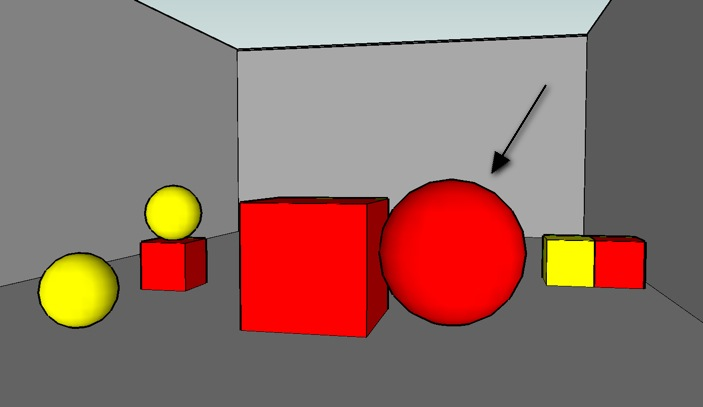
\includegraphics[width=0.6\textwidth]{images/22sinletras.jpg}
\caption{Ejemplo de contexto}
\label{GRE3D7-stimulus}
\end{figure}

Una propiedad es una caracter\'istica propia de un objeto. Por ejemplo en el Contexto \ref{GRE3D7-stimulus} el objeto se\~nalado con la flecha tiene la propiedad {\it color} con valor {\it rojo}. Por simplicidad, en el resto de la tesis vamos a decir ``tiene propiedad {\it rojo}'', cuando queremos decir que el objeto tiene la propiedad color con valor rojo. Una relaci\'on caracteriza a un objeto describiendo caracter\'isticas de otro u otros objetos.\\

%Cuando la ER no es relacional solo contiene propiedades del objeto mismo. Ej.: color, tama\~no. Note que quiz\'as el tama\~no sea con respecto a los dem\'as objetos ``la m\'as peque\~na'', pero al no incluir una descripci\'on de otro objeto no la llamamos relacional.\\
De acuerdo a las propiedades o relaciones que una expresi\'on referencial (ER) incluya, se clasifican en distintos tipos: relacional o no relacional (tambi\'en llamada proposicional), m\'inima, sobreespecificada, o subespecificada. A continuaci\'on describimos cada uno de estos tipos.\\

% en cuyo caso es una expresi\'on que no es referencial, la incluimos en nuestras propiedades porque nos va a ser \'util la definici\'on en el Cap\'itulo \ref{sec:corpus}.\\
Una ER {\it proposicional} o no relacional, incluye s\'olo propiedades intr\'insecas del objeto target. Por ejemplo en el Contexto \ref{GRE3D7-stimulus}: ``La pelota roja''. Las caracter\'isticas de ser pelota, ser roja son propias del objeto identificado.\\

Una ER es {\it relacional}, cuando adem\'as de ser proposicional, contiene relaciones con otros objetos, entonces la ER incluye las ERs de los otros objetos.  Por ejemplo en el Contexto \ref{GRE3D7-stimulus}: ``La pelota que esta a la derecha del cubo grande'', ``a la derecha de'' es una relaci\'on que necesita describir otro objeto adem\'as del target, en este caso ``el cubo grande''.\\

Se dice que una ER es {\it minimal}, cuando incluye la m\'inima cantidad de propiedades con las cuales el objeto puede ser distinguido en el contexto dado. Notar que puede haber muchas expresiones minimales. Por ejemplo en el Contexto \ref{GRE3D7-stimulus} ``La pelota roja'' es una ER minimal, como as\'i tambi\'en lo es ``La pelota grande'', ya que ambas tienen 2 propiedades, y 2 es la m\'inima cantidad de propiedades que puede tener una ER de ese objeto, para distinguirlo en ese contexto.\\

Cuando la ER contiene m\'as informaci\'on de la m\'inima necesaria para distinguirlo de los dem\'as objetos en el contexto dado, se dice que la ER es {\it sobreespecificada}. Por ejemplo: ``La pelota roja grande'' en el Contexto \ref{GRE3D7-stimulus}.\\

Una expresi\'on es {\it subespecificada} cuando no alcanza a ser una ER, ya que no se puede distinguir al objeto target de todos los objetos en el contexto. Por ejemplo: ``La pelota'' en el Contexto \ref{GRE3D7-stimulus} no alcanza para distinguir el objeto apuntado por la flecha, ya que hay otras 2 pelotas. En estos casos se debe dar otra expresi\'on o corregir la anterior agregando m\'as propiedades o relaciones. Una expresi\'on subespecificada identifica a un conjunto, no a un objeto \'unico.

\section{La tarea de generaci\'on autom\'atica de expresiones referenciales}

La generaci\'on autom\'atica de expresiones referenciales (GER), es la tarea de definir cuales pasos se deben seguir para conseguir una ER de un objeto espec\'ifico, en un contexto dado. Estos pasos definen un algoritmo de GER. \\

Los algoritmos se pueden diferenciar por la cantidad y forma de los par\'ametros que toman como input, es decir el modo en que toman por ejemplo el contexto para el cual se espera que den una expresi\'on referencial. \\

En todos los casos, la computadora necesita tener un conjunto de propiedades/relaciones para cada objeto y poder identificarlos, para ello vamos a etiquetar a los objetos con $e_1$, $e_2$, etc. como se muestra en la Figura \ref{GRE3D7-stimulus-conLetras}. En la imagen tambi\'en podemos ver que el objeto se\~nalado con la flecha es $e_5$, es el objeto target, para el cual queremos generar autom\'aticamente una expresi\'on referencial.

\begin{figure}[ht]
\centering
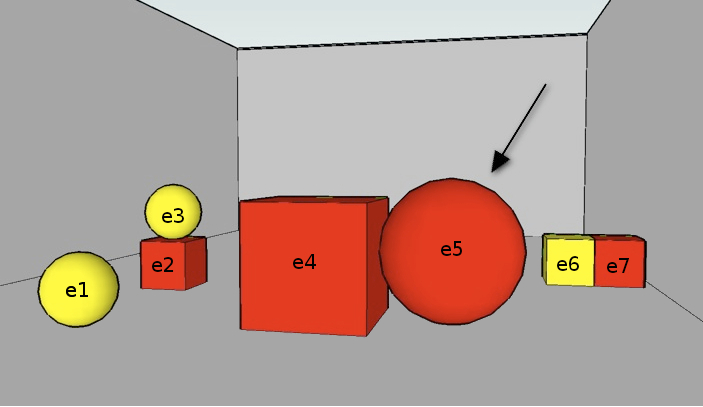
\includegraphics[width=0.6\textwidth]{images/22.jpg}
\caption{Ejemplo de contexto con objetos etiquetados}
\label{GRE3D7-stimulus-conLetras}
\end{figure}

A continuaci\'on daremos 2 ejemplos de diferentes maneras de modelar el contexto que toman como input, uno para el algoritmo Graph y otro para algoritmo de Bisimulaci\'on.\\

%El contexto que toma como input el algoritmo GRAPH \cite{graph08} el cual explicaremos en la Secci\'on \ref{graph}, para el Contexto \ref{GRE3D7-stimulus}, es un grafo dirigido y etiquetado como se muestra en Figura \ref{grafo-GRE3D7-stimulus}, el cual contiene la informaci\'on de las propiedades y relaciones de los objetos, por ejemplo podemos ver que el objeto target que es el $e_5$, tiene propiedades large, red, ball y una flecha con la etiqueta rightof $e_4$, y $e_4$ tiene propiedades large, red, cube, y una flecha hacia $e_5$ con etiqueta leftof.\\

El contexto que toma como input el algoritmo Graph \cite{graph08} el cual explicaremos en la Secci\'on \ref{graph}, para el Contexto \ref{GRE3D7-stimulus}, es un grafo dirigido y etiquetado como se muestra en Figura \ref{grafo-GRE3D7-stimulus}, el cual contiene la informaci\'on de las propiedades y relaciones de los objetos, por ejemplo podemos ver que el objeto $e_5$, tiene propiedades grande, rojo, pelota y una flecha con la etiqueta a-la-derecha-de hacia $e_4$, y $e_4$ tiene propiedades grande, rojo, cubo, y una flecha hacia $e_5$ con etiqueta a-la-izquierda-de.\\

\begin{figure}[ht]
\centering
\begin{tikzpicture}
  [
    n/.style={circle,fill,draw,inner sep=3pt,node distance=2cm},
    aArrow/.style={->, >=stealth, semithick, shorten <= 1pt, shorten >= 1pt},
  ]
 \node[n,label=above:$e_1$,label=below:{
    \relsize{-2}$\begin{array}{c}
      \nSmall\\[-3pt] 
      \nYellow \\[-3pt] 
      \nBall\end{array}$}] (a) {};
 \node[n,label=above:$e_2$,label=below:{
    \relsize{-2}$\begin{array}{c}     
      \nSmall\\[-3pt] 
      \nRed\\[-3pt] 
      \nCube\end{array}$}, right of=a] (b) {};
 \node[n,label=below:$e_3$,label=above:{
    \relsize{-2}$\begin{array}{c}
      \nTop\\[-3pt]      
      \nSmall\\[-3pt] 
      \nYellow\\[-3pt] 
      \nBall\end{array}$}, above of=b] (c) {};
 \node[n,label=right:$e_4$,label=left:{
    \relsize{-2}$\begin{array}{c}
      \nLarge\\[-3pt] 
      \nRed\\[-3pt] 
      \nCube\end{array}$}, right of=b] (d) {};
 \node[n,label=left:$e_5$,label=below:{
    \relsize{-2}$\begin{array}{c}
      \nLarge\\[-3pt] 
      \nRed\\[-3pt] 
      \nBall\end{array}$}, right of=d] (e) {};
 \node[n,label=right:$e_6$,label=left:{
    \relsize{-2}$\begin{array}{c}
      \nSmall\\[-3pt] 
      \nYellow\\[-3pt] 
      \nCube\end{array}$}, right of=e] (f) {};
 \node[n,label=left:$e_7$,label=below:{
    \relsize{-2}$\begin{array}{c}
      \nSmall\\[-3pt]
      \nRed\\[-3pt] 
      \nCube\end{array}$},  right of=f] (g) {};
 \draw [aArrow,bend right=40] (b) to node[auto,swap]{\relsize{-3}$\nBelow$} (c);
 \draw [aArrow,bend right=40] (c) to node[auto,swap]{\relsize{-3}$\nOntop$} (b);
 \draw [aArrow,bend right=40] (d) to node[auto,swap]{\relsize{-3}$\nLeftof$} (e);
 \draw [aArrow,bend right=40] (e) to node[auto,swap]{\relsize{-3}$\nRightof$} (d);
 \draw [aArrow,bend right=40] (f) to node[auto,swap]{\relsize{-3}$\nLeftof$} (g);
 \draw [aArrow,bend right=40] (g) to node[auto,swap]{\relsize{-3}$\nRightof$} (f);
 \draw[dotted] (-0.5,-1.1) rectangle (10.5,3.1);

 \end{tikzpicture}
\caption{Grafo del contexto \ref{GRE3D7-stimulus}}
\label{grafo-GRE3D7-stimulus}
\end{figure}

Para el mismo Contexto \ref{GRE3D7-stimulus-conLetras}, el input del algoritmo de Bisimulaci\'on el cual explicaremos en Secci\'on \ref{bisimulacion}, es un archivo con formato XML \footnote{XML, siglas en ingl\'es de eXtensible Markup Language ('lenguaje de marcas extensible'), es un lenguaje de marcas desarrollado por el World Wide Web Consortium (W3C) utilizado para almacenar datos en forma legible.} con la misma informaci\'on del Contexto \ref{input-bisimulacion}. En este caso se representan las propiedades como relaciones a un objeto ficticio, terminal {\it c}, creado para modelar propiedades y relaciones, como relaciones, como veremos luego esto va a servir para dar prioridad a las relaciones en algunos casos. En el XML podemos ver que todos los objetos tienen ``id'' que es el identificador, salvo el objeto target $e_5$ el cual tiene {\it refer-to} en vez de {\it id}. Con la etiqueta ``rel'', identificamos las relaciones y con la etiqueta ``to'' con que objeto esta relacionado. El target tiene relaciones con c (grande, rojo, pelota) y con $e_4$ a-la-derecha-de.  
%\'Este tiene las relaciones con c (large, red, ball) y con $e_4$ rightof.  
\textcolor{blue}{aca tengo problemas en verbatim para escribir la enie de pequeino}
\label{input-bisimulacion}

%\include{xml}

\begin{verbatim}
<?xml version="1.0"?>
<problem id="e1">c
  <individual id="e1">
    <related rel="pequeno" to="c" />
    <related rel="amarillo" to="c" />
    <related rel="pelota" to="c" />
  </individual>
  ...
  <individual id="e4">
    <related rel="cubo" to="c" />
    <related rel="rojo" to="c" />
    <related rel="grande" to="c" />
    <related rel="a-la-izquierda-de" to="e5" />
  </individual>
  <individual refer-to="e5">
    <related rel="grande" to="c"/>
    <related rel="pelota" to="c" />
    <related rel="rojo" to="c" />
    <related rel="a-la-derecha-de" to="e4" />
  </individual>
  ...
  <individual id="c">
    <related rel="terminal" to="c" />
  </individual> 
</problem>
\end{verbatim}
%\label{input-bisimulacion}
%\begin{verbatim}
%<?xml version="1.0"?>
%<problem id="e1">c
  %<individual id="e1">
    %<related rel="small" to="c" />
    %<related rel="yellow" to="c" />
    %<related rel="ball" to="c" />
  %</individual>
  %...
  %<individual id="e4">
    %<related rel="cube" to="c" />
    %<related rel="red" to="c" />
    %<related rel="large" to="c" />
    %<related rel="left-of" to="e5" />
  %</individual>
  %<individual refer-to="e5">
    %<related rel="large" to="c"/>
    %<related rel="ball" to="c" />
    %<related rel="red" to="c" />
    %<related rel="right-of" to="e4" />
  %</individual>
  %...
  %<individual id="c">
    %<related rel="terminal" to="c" />
  %</individual> 
%</problem>
%\end{verbatim}
%Saque para que no quede tan largo
%<individual id="e6">
    %<related rel="small" to="c" />
    %<related rel="cube" to="c" />
    %<related rel="yellow" to="c" />
    %<related rel="left-of" to="e7" />
  %</individual>
  %<individual id="e7">
    %<related rel="small" to="c" />
    %<related rel="cube" to="c" />
    %<related rel="red" to="c" />
    %<related rel="right-of" to="e6" />
  %</individual>

%<individual id="e2">
%    <related rel="cube" to="c" />
%    <related rel="red" to="c" />
%    <related rel="small" to="c" />
%    <related rel="bellow" to="e3" />
%  </individual>
%  <individual id="e3">
%    <related rel="ball" to="c" />
%    <related rel="yellow" to="c" />
%    <related rel="small" to="c" />
%    <related rel="on-top" to="e2" />
%  </individual>
Los algoritmos tambi\'en se pueden diferenciar por la clase de ER que pueden generar, a continuaci\'on explicaremos los distintos tipos de algoritmos de GER. 

\section{Tipos de algoritmos de GER}

Un algoritmo para la generaci\'on autom\'atica de expresiones referenciales  puede ser: determin\'{i}stico o no-determin\'{i}stico, relacional o proposicional, incluir negaciones o no, identificar plurales o s\'olo singulares,
 %usar disyunciones y conjunciones, o s\'olo conjunciones, 
generar ER sobreespecificadas o minimales.  A continuaci\'on se describen cada uno de esos tipos.\\

Un algoritmo es {\it determin\'{i}stico} si dado un input (un contexto y un objeto target), da siempre la misma ER de salida. En cambio un algoritmo es {\it no-determin\'{i}stico} si es posible que d\'e distintas salidas para el mismo input, en distintas ejecuciones. En general las personas generan expresiones referenciales de forma no determin\'istica, por lo tanto los algoritmos no determin\'isticos simulan el comportamiento de distintas personas, o incluso el de la misma persona en distintos momentos. Por ejemplo ser\'ia no determin\'istico si para el Contexto \ref{GRE3D7-stimulus-conLetras} una vez da ``La pelota roja'' y en otra ejecuci\'on ``La pelota grande''.\\

Un algoritmo es {\it proposicional}, cuando las ER que genera contienen solo atributos del target, es decir no contiene relaciones con otros atributos ni ER de otros objetos.  Por ejemplo para el Contexto \ref{GRE3D7-stimulus-conLetras} una vez da ``La pelota roja''.\\

Un algoritmo es {\it relacional} si adem\'as de generar ER proposicionales genera ER relacionales, en cuyo caso adem\'as de generar las relaciones correspondientes deber\'a generar ERs para el o los objetos relacionados. Por ejemplo para el Contexto \ref{GRE3D7-stimulus-conLetras} la ER ``La pelota roja a la derecha del cubo grande''. En este caso ``el cubo grande'' es una expresi\'on referencial que se tuvo que dar como consecuencia de incluir la relaci\'on ``a la derecha de''.\\

En algunos contextos cuando el target es el \'unico que no tiene una propiedad por ejemplo, ser\'ia \'util un algoritmo que incluya {\it negaciones}. Por ejemplo para el Contexto \ref{GRE3D7-stimulus-conLetras}, ``La \'unica pelota que no es peque\~na''.\\

Un algoritmo puede generar ER para {\it plurales}, es decir dar ER para varios targets en el contexto considerado. Por ejemplo para el Contexto \ref{plurales}, ``Los objetos grandes''. En este caso el target no es \'unico, sino un conjunto de objetos. \\

\begin{figure}[ht]
\centering
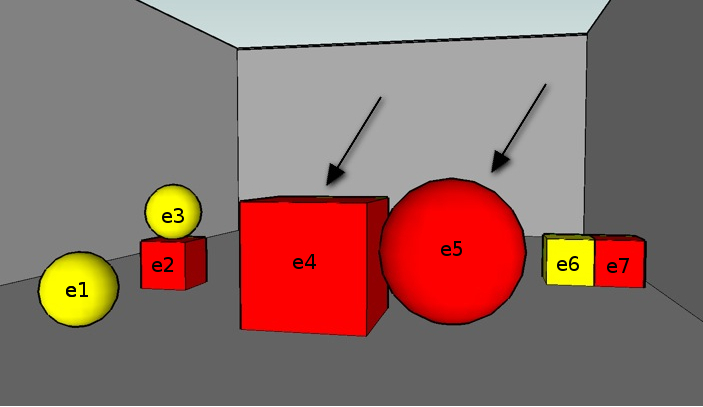
\includegraphics[width=0.6\textwidth]{images/22-plural.jpg}
\caption{Ejemplo de contexto con 2 targets}
\label{plurales}
\end{figure}
%esto lo saque porque confunde aca... me parece que todavia no hay que hablar de esto, es muy de logica
%Los algoritmos tambi\'en se pueden diferenciar en los conectores que permiten si usan conjunciones, disyunciones o ambas.\\

Un algoritmo que genera ER {\it minimales}, es un algoritmo que da ER que contienen la m\'inima cantidad de propiedades o relaciones que se necesitan para distinguir al target.  Por ejemplo para el Contexto \ref{GRE3D7-stimulus-conLetras} ``La pelota grande''.\\

La {\it sobreespecificaci\'on} es la caracter\'istica de dar m\'as atributos o relaciones de las necesarias para identificar al objeto target. Por ejemplo para el Contexto \ref{GRE3D7-stimulus-conLetras} la ER ``La pelota roja, grande que esta a la derecha del cubo rojo grande'' es una ER sobreespecificada.\\

%no se si dejar esto...
%Un algoritmo que hace backtraking, es el que luego de incluir una propiedad o relaci\'on puede deshacer esa inclusi\'on volviendo a un estado anterior, es decir, decidir no incluirla.\\

\section{Algoritmos importantes en el \'area}
%interesante...
%https://www.abdn.ac.uk/ncs/departments/computing-science/tunabibl-495.php

En esta secci\'on vamos a hablar de los algoritmos de generaci\'on autom\'atica de expresiones referenciales, empezando por el algoritmo Full Brevity, el algoritmo de heur\'istica Greedy, siguiendo con el algoritmo Incremental, Graph, algoritmo Relacional y por \'ultimo Bisimulaci\'on.  \\

%http://citeseerx.ist.psu.edu/viewdoc/download?doi=10.1.1.227.8284&rep=rep1&type=pdf

%REG can be traced back to the earliest days of Natural Language Processing; Winograd
%(1972)  (Section  8.3.3,  Naming  Objects  and  Events),  for  example,  sketches  a  primitive
%“incremental” REG algorithm, used in his SHRDLU program. In the 1980s, researchers
%such as Appelt and Kronfeld set themselves the ambitious task of modelling the human
%capacity for producing and understanding referring expressions in programs such as
%KAMP and BERTRAND (Appelt 1985; Appelt and Kronfeld 1987; Kronfeld 1990). They
%argued that referring expressions should be studied as part of a larger speech act. KAMP
%(Appelt  1985),  for  example,  was  conceived  as  a  general  utterance  planning  system,
%building  on  Cohen  and  Levesque’s  (1985)  formal  speech  act  theory.

%REG  task  is  now  defined  by  Dale  and  Reiter  (1995)  through  what  may  be
%called identification of the target: given a target (or referent) object r 2 D , find a set of attribute–value  pairs L
%whose  conjunction  is  true  of  the  target  but  not  of  any  of  the
%distractors (i.e., D

%Full  Brevity  and  Greedy  Heuristic.
El algoritmo {\it Full Brevity} \cite{Dale:1989:CUR:981623.981632} genera la descripci\'on m\'as corta que identifica al target. Para hacerlo, 
busca si hay una propiedad del target que no sea propiedad de ning\'un distractor. Si no hay chequea todas las posibles combinaciones de 2 propiedades, si no la hay, busca de a 3 y as\'i sucesivamente.\\

El problema es que encontrar la descripci\'on m\'as corta es de alta complejidad, se observ\'o que las personas dan expresiones que no son minimales, esto fue confirmado por estudios psycoling\"uisticos (\cite{Olson1970LangAndThought};  \cite{Sonnenschein1984}; \cite{Pechmann1989}; \cite{Engelhardt2006}).\\

Una aproximaci\'on a Full Brevity es el algoritmo de heur\'istica {\it Greedy}, el cual iterativamente selecciona la propiedad que elimina m\'as distractores y argumentan que la propiedad seleccionada tiene el m\'as alto poder discriminativo en esa etapa. Como resultado no siempre genera expresiones referenciales m\'inimas.\\

%which  iteratively  selects  the  property  which  rules  out  most  of  the  distractors
%not  previously  ruled  out,  incrementally  augmenting  the  description  based  on  what
%property has most discriminatory power at each stage (as a result, it does not always
%generate  descriptions  of  minimal  size). 
El algoritmo de heur\'istica Greedy es m\'as eficiente que el Full Brevity, pero pronto fue superado por el algoritmo {\it Incremental} y sus sucesores \cite{C92-1038}; \cite{Dale95computationalinterpretations}. El algoritmo Incremental fue y sigue siendo uno de los algoritmos m\'as importantes del \'area, lo explicamos a continuaci\'on. 
% The  Greedy  Heuristic  algorithm  is  a  more
%efficient  algorithm  than  the  Full  Brevity  one,  but  it  was  soon  eclipsed  by  another
%algorithm    which  turned  out  to  be  the
%most influential algorithm of the pre-2000 era. It is this later algorithm that came to be
%known as``the'' Incremental Algorithm (IA).

%\subsection{GREEDY}

%El algoritmo GREEDY de Dale~\cite{dale89} busca sobre todo el conjunto de propiedades del target y elije el subconjunto m\'as chico posible que identifica un\'{i}vocamente al objeto target entre los distractores en la escena considerada como se muestra en el siguiente algoritmo.\\

%\begin{figure}[ht]
%\begin{center}
%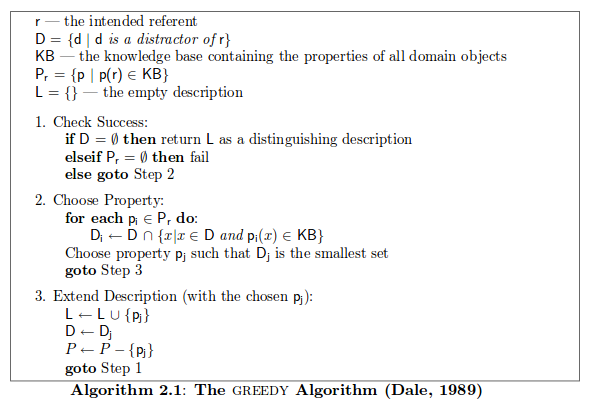
\includegraphics[width=8.5cm]{figures/greedy.png}\\[0pt]
%\caption{Interface del experimento}
%\label{fig-greedy}
%\end{center}
%\end{figure}

%r - el objeto target\\
%D = \{d|d es un distractor de r\}\\
%KB - la base de conocimiento que contiene las propiedades de todos los objetos\\
%$P_{r}$ = $\{p|p(r) \in KB\}$\\
%L = $\{\}$ - la descripci\'on vac\'{i}a\\
%\\
%1. Chequea \'exito:\\
%    \textbf{if} D = $\emptyset$ \textbf{then} return L como una ER que distingue al target r
%    \textbf{elseif} $P_{r}$ = $\emptyset$ \textbf{then} fail
%    
%\textbf{else goto} Paso 2 \\
%\\
%2. Elegir Propiedad:
% \textbf{for each} $p_{i}$ $\in$ $P_{r}$ \textbf{do}:
%    $D_{i}$ $\leftarrow$ D$\cap$ \{x|x $\in$ D and $p_{i}$ (x) $\in$ KB\}
%    Elegir la propiedad $p_{j}$ tal que $D_{j}$ es el conjunto m\'as chico (es decir la que elimina m\'as distractores) \textbf{goto} Paso 3\\
%\\    
%3. Agregar $p_{j}$ a la descripci\'on actual\\
%L $\leftarrow$ L $\cup$ \{$p_{j}$\}\\
%D $\leftarrow$ $D_{j}$\\
%P $\leftarrow$ P -\{$p_{j}$\}\\
%\textbf{goto} Paso 1\\



%%Dado un dominio D que contiene un target referente r y un conjunto de distractores, una base de conocimiento KB que contiene las propiedades de los objetos.
%%Un conjunto de propiedades verdaderas para r, y una descripcion L inicialmente vac\'{i}a.

%Este algoritmo es de orden NP-complete

\subsection{Incremental}

%A continuaci\'on se describe el algoritmo Incremental de Dale \& Reiter el cual esta basado en el algoritmo GREEDY (el cual hac\'ia una b\'usqueda exaustiva y eleg\'ia la propiedad que m\'as distractores eliminaba en cada paso) pero \'este reduce la complejidad del algoritmo Greedy cambiando que en vez de chequear cual propiedad es la que elimina m\'as distractores, eligiendo la que sigue en la lista de propiedades ordenada seg\'un preferencia y que elimina al menos un distractor. Este algoritmo es de orden polinomial. Este algoritmo produce expresiones referenciales que pueden estar sobreespecificadas.\\

\textcolor{blue}{error entorno matematico, pero no entiendo porque, y no puedo hacer que diga algoritmo en vez de algorithm}

%\begin{figure}
\small
\begin{center}
%\centering
\begin{algorithm}[H]

\dontprintsemicolon

\captionsetup[algorithm]{name=Algoritmo}
\caption{Incremental\label{algo:incremental}}
%\caption{Incremental}\label{algo:incremental}
\KwIn{\footnotesize \{r, D, Pref\} r es el target, D es el dominio, Pref lista de preferencia de propiedades ordenadas}
\KwOut{\footnotesize L  - Descripci\'on de salida}

$\ L \leftarrow \emptyset $ \tcp*[f]{\footnotesize Inicialmente es vac\'io}\\
$\ C \leftarrow D - \{r\} $ \tcp*[f]{\footnotesize C es el conjunto de todos los objetos menos r }\\


\For{\em $A_{i} \in Pref$ }{
	$V = Value(r,A_{i})$ \tcp*[f]{\footnotesize V es el valor de la propiedad $A_{i}$ para r }\\
	\If(\tcp*[f]{\footnotesize Si elimina alg\'un distractor}){\em $C \cap RulesOut(\[A_{i}\],V) \neq \emptyset $}
	{
    $\ L \leftarrow L \cup \{A_{i},V\} $  \tcp*[f]{\footnotesize Agrega la propiedad $A_{i}$ a L }\\
    $\ C \leftarrow C - RulesOut(\[A_{i}\],V) $  \tcp*[f]{\footnotesize Actualiza C sacando los objetos que no tienen V en $A_{i}$} 
    }
    \If(\tcp*[f]{\footnotesize Si no quedan distractores}){\em $C = \emptyset $}
	  {
     Return L  
    }
  }
Return Fallo
\end{algorithm}
\end{center}
%\end{figure}



Como podemos ver en \ref{algo:incremental} el input de este algoritmo es el objeto target que queremos identificar {\it r}, D, el dominio, y Pref una lista ordenada de preferencia de propiedades.\\
En {\it Paso 1} se asigna a L la descripci\'on vac\'{i}a, al finalizar la ejecuci\'on, L tendr\'a el conjunto de propiedades con los cuales identificaremos a r, es decir una expresi\'on referencial de r. 
Se le asigna a C el conjunto de distractores de r (todos los objetos menos r), en {\it Paso 2}.\\

La idea del algoritmo es ir eliminando distractores, por eso, en el {\it Paso 3} recorre las propiedades de r. En {\it Paso 4} le asigna a V el valor que tiene el target para la propiedad $A_{i}$

$RulesOut(A_{i},V)$ devuelve el conjunto de objetos que tienen diferente valor para la propiedad $A_{i}$ que el que tiene el objeto target.

Si hay objetos en C que tengan diferente valor de $A_{i}$ que el target, se agrega la propiedad a la descripci\'on actual L en {\it Paso 6}, y se actualiza $C$ sacando los objetos que no tienen V en $A_{i}$. 

Luego en {\it Paso 8} si C es $\emptyset$ (si no hay m\'as distractores) devolvemos L, como el conjunto de propiedades que identifican a r.

Vamos a ejemplificar la corrida del algoritmo con el ejemplo de Contexto \ref{GRE3D7-stimulus-conLetras}, y supongamos que la lista ordenada de propiedades es esta [ tipo, color, tama\~no ]. D inicialmente es \{$e_{1}$,$e_{2}$,$e_{3}$,$e_{4}$,$e_{5}$,$e_{6}$,$e_{7}$\}
Al iniciar a L le asigna $\emptyset$ y a C \{$e_{1}$,$e_{2}$,$e_{3}$,$e_{4}$,$e_{6}$,$e_{7}$\}, luego comienza a recorrer la lista de propiedades, la primer propiedad es ``tipo'', el valor del target para tipo es {\it pelota}, entonces en {\it Paso 6}, pregunta si hay objetos que tengan tipo con valor distinto de pelota, y hay, ellos son \{$e_{2}$,$e_{4}$,$e_{6}$,$e_{7}$\}, entonces le asigna a C \{$e_{1}$,$e_{3}$\}, es decir solo las pelotas. En {\it Paso 10} pregunta si C es vac\'io, no lo es, por lo tanto continua con la siguiente propiedad, en este caso ``color'', el valor de color para el target es {\it rojo}, agrega {\it rojo} a L, y actualiza C con $\emptyset$ porque tanto $e_{1}$ como $e_{3}$ son amarillos, en {\it Paso 10} pregunta si C es vac\'io, y si lo es, por lo tanto devuelve \{pelota, rojo\}.


%Intuitivamente, si la primer propiedad tipo y el valor de tipo para el target es ``pelota'', nos quedamos con todos los objetos pelota.\\

%\textcolor{blue}{Un poco mas de historia, no se a donde poner...Theune and Krahmer proposed an extension that allows the generation of subsequent reference with the ia taking into account the discourse salience of the target referent (Krahmer and Theune, 1998; Theune, 2000; Krahmer and Theune, 2002), and a second one which allows the ia to produce referring expressions that
%contain binary relations to other objects (Theune, 2000; Krahmer and Theune, 2002). I will return to their relational extension in Section 2.3. Theune and Krahmer's approach works by assigning a salience score to all objects according to the
%focus/topic distinction by Hajicova (1993) and Centering Theory (Grosz et al., 1995). They alter the success criterion of the algorithm and only let it stop when here is no distractor left that is as or more salient than the target referent.
%Not all properties are the same. The qualitative diferences that exist between diferent properties were first discussed in the
%reg literature by van Deemter (2000, 2006). He pointed out that the appropriateness of
%vague orgradable properties such as small and large is dependent on the context in which they are used, while,
%for example, the colour of an object is absolute. Consider two descriptions in a domain of animals... (van Deemter, 2002), van Deemter considered the ia's logical completeness in terms of the Boolean operators of negation and disjunction. He extended it to
%be able to generate referring expressions that contain negated properties, such as Example (2.3), and descriptions of sets of objects, such as Example (2.4), or even (2.5), which contains a logical disjunction of properties. His algorithm proceeds
%in stages, trying longer and longer disjunctions of properties, if atomic properties
%and shorter disjunctions did not suffice to distinguish the target set.. he work on reference to sets was taken further by Gatt and van Deemter (2005, 2006), who have presented the most mature algorithms in this space to
%date. They used a similar procedure to the ia in that their algorithms are based
%on incremental processing of a preference order of properties. Their algorithms
%add a lot of complex machinery to the basic procedure to ensure that properties
%are chosen in a way that maximises coherence within the set of objects described
%by the referring expressions. For example, their approach will attempt to use
%properties of the same type for all the referents of a set. So, it would produce
%descriptions such as Examples 
Luego se propusieron extensiones del algoritmo Incremental, por ejemplo 
Theune y Krahmer propusieron una extensi\'on que permite la generaci\'on de referencia teniendo en cuenta la prominencia discurso del target (\cite{Krahmer:2010:EMN:1880370}; \cite{krahmer-theune:2002a};), y un segundo algoritmo que permite producir expresiones referenciales que contienen relaciones con otros objetos. El enfoque Theune y de Krahmer funciona asignando una puntuaci\'on de relevancia a todos los objetos de acuerdo con el enfoque / tema distinci\'on por \cite{hajicova-1993} y la teor\'ia de centrado \cite{Grosz:1995:CFM:211190.211198}. Alteran el criterio de \'exito del algoritmo y s\'olo permiten que se detenga cuando hay un distractor que es tanto o m\'as relevante que el target.
No todas las propiedades tienen la misma relevancia. Las diferencias cualitativas que existen entre diferentes propiedades se discutieron por primera vez en la literatura GER por van Deemter (2000, 2006). Se\~nal\'o que la conveniencia de otras propiedades sobre las
propiedades vagas como peque\~no y grande dependen del contexto en el que se utilizan, mientras que, por ejemplo, el color de un objeto es absoluta. 
%Considere dos descripciones de un dominio de los animales ... (van Deemter, 2002), van Deemter considera integridad l\'ogica del ia en t\'erminos de los operadores booleanos de negaci\'on y disyunci\'on. \'el la extendi\'o a
%ser capaz de generar expresiones referenciales que contienen propiedades, tales como Ejemplo (2.3) negado, y las descripciones de conjuntos de objetos, tales como Ejemplo (2.4), o incluso (2,5), que contiene una disyunci\'on l\'ogica de propiedades. Sus algoritmo procede
%en etapas, tratando m\'as y disyunciones m\'as largos de propiedades, si las propiedades at\'omicas
%y disyunciones m\'as cortos no son suficientes para distinguir el conjunto target .. que funciona en referencia a conjuntos fue tomada adem\'as por Gatt y van Deemter (2005, 2006), que han presentado los algoritmos m\'as maduros a la fecha. Utilizaron un procedimiento similar al de las otras cosas en que sus algoritmos se basan en el procesamiento incremental de un orden de preferencia de las propiedades. Sus algoritmos agregan una gran cantidad de maquinaria compleja para el procedimiento b\'asico para asegurar que las propiedades
%se eligen de manera que maximiza la coherencia dentro del conjunto de objetos descritos por las expresiones referenciales. Por ejemplo, su enfoque intentar\'a utilizar propiedades del mismo tipo para todos los referentes de un conjunto. As\'i, ser\'ia producir
%descripciones tales como ejemplos
%(2.6) or (2.7) rather than Example (2.8) or.. 


%Theune y Krahmer propusieron una extensi\'on que permite la generaci\'on de referencia con la subsiguiente ia teniendo en cuenta la prominencia discurso del referente objetivo (Krahmer y Theune, 1998; Theune, 2000; Krahmer y Theune, 2002), y un segundo uno que permite la IA para producir expresiones referenciales que contener relaciones binarias a otros objetos (Theune, 2000; Krahmer y Theune, 2002). Voy a volver a su extensi\'on relacional en la Secci\'on 2.3. Enfoque Theune y de Krahmer funciona asignando una puntuaci\'on de relevancia a todos los objetos de acuerdo con la enfoque / tema distinci\'on por Hajicova (1993) y el centrado Theory (Grosz et al., 1995). Alteran el criterio de \'exito del algoritmo y s\'olo permiten que se detenga cuando aqu\'i hay izquierda distractor que es tan o m\'as relevante que el referente de destino.
%No todas las propiedades son las mismas. Las Diferencias cualitativas que existen entre diferentes propiedades se discutieron por primera vez en la literatura reg por van Deemter (2000, 2006). Se\~nal\'o que la conveniencia de propiedades orgradable vagos como peque\~nos y grandes depende del contexto en el que se utilizan, mientras que, Por ejemplo, el color de un objeto es absoluta. Considere dos descripciones de un dominio de los animales ... (van Deemter, 2002), van Deemter considera integridad l\'ogica del ia en t\'erminos de los operadores booleanos de negaci\'on y disyunci\'on. \'el la extendi\'o a ser capaz de generar expresiones que se refieren que contienen propiedades, tales como Ejemplo (2.3) negado, y las descripciones de conjuntos de objetos, tales como Ejemplo (2.4), o incluso (2,5), que contiene una disyunci\'on l\'ogica de propiedades. Sus algoritmo procede en etapas, tratando m\'as y disyunciones m\'as largos de propiedades, si las propiedades at\'omicas y disyunciones m\'as cortos no son suficientes para distinguir el conjunto de destino .. que funciona en referencia a conjuntos fue tomada adem\'as por Gatt y van Deemter (2005, 2006), que han presentado los algoritmos m\'as maduros en este espacio para la fecha. Utilizaron un procedimiento similar al de las otras cosas en que sus algoritmos se basan en el procesamiento incremental de un orden de preferencia de las propiedades. Sus algoritmos agregar una gran cantidad de maquinaria compleja para el procedimiento b\'asico para asegurar que las propiedades se eligen de manera que maximiza la coherencia dentro del conjunto de objetos descritos por las expresiones que se refieren. Por ejemplo, su enfoque intentar\'a utilizar propiedades del mismo tipo para todos los referentes de un conjunto. As\'i, ser\'ia producir Ejemplos descripciones tales como (2,6) o (2,7) en lugar de Ejemplo (2.8) o ..


\subsection{Algoritmo de b\'usqueda en Grafo}
\label{graph}
%Un grafo es un conjunto de objetos llamados v\'ertices o nodos unidos por enlaces llamadas aristas o arcos, que permiten representar relaciones binarias entre elementos de un conjunto. \\

Un grafo G es un par ordenado $G=(V,E)$, donde:
\begin{itemize}
   \item V es un conjunto de v\'ertices o nodos, y
    \item E es un conjunto de aristas o arcos, que relacionan estos nodos.

%\item Se llama orden del grafo G a su n\'umero de v\'ertices, $|V|$.

%\item El grado de un v\'ertice o nodo $v \in V$ es igual al n\'umero de arcos que lo tienen como extremo.

%\item Un bucle es una arista que relaciona al mismo nodo; es decir, una arista donde el nodo inicial y el nodo final coinciden.

%\item Dos o m\'as aristas son paralelas si relacionan el mismo par de v\'ertices.

%\item Un grafo puede ser dirigido o no, etiquetado o no.
\end{itemize}
%T\'{i}picamente, un grafo se representa gr\'aficamente como un conjunto de puntos (v\'ertices o nodos) unidos por l\'{i}neas (aristas).

Los grafos han sido muy estudiados, pr\'acticamente cualquier problema puede ser expresado como un problema de grafos, y aplicar algoritmos de b\'usqueda ya estudiados.

El algoritmo Graph de \cite{Krahmer:2003} propone ver la obtenci\'on de expresiones referenciales como un problema de grafos, el contexto que incluye al target y los distractores es representado como un grafo. \\

Cada objeto de la escena se modela como un v\'ertice en el grafo. Las propiedades at\'omicas como color, tipo o tama\~no se representan como un bucle en el correspondiente nodo. Est\'an etiquetados con los nombres de las propiedades y los valores que el objeto en cuesti\'on tiene para estas propiedades. \\

Las relaciones binarias entre objetos, por ejemplo abajo-de, arriba-de se modelan como aristas entre los nodos correspondientes.\\

%La base de conocimiento que incluye al target ahora esta expresada como los v\'ertices, las aristas y las etiquetas del grafo.\\

%Krahmer et al.'s (2003) reformularon la tarea de seleccionar las propiedades y relaciones que contendr\'a una expresi\'on referencial como un problema de teor\'ia de grafos.

Para generar una descripci\'on distintiva, el algoritmo busca un subgrafo del grafo original que identifica al target un\'{i}vocamente, le llama grafo distintivo.\\% (distinguishing graph).\\

Comenzando con el subgrafo que contiene un solo v\'ertice, que representa al target, se realiza una b\'usqueda exhaustiva, pero comenzando a lo ancho. Utiliza una heur\'{i}stica basada en el costo (costo de incluir propiedades, relaciones) para podar el espacio de b\'usqueda. Y da el grafo de menor costo. \\


%esto no se entiende nada
%Informalmente, un subgrafo refiere al target si y s\'olo si puede ser
%`Colocado sobre el gr\'afico de dominio de tal manera que el v\'ertice que representa subgrafo
%del objeto target se puede `coloca sobre 'el v\'ertice del objetivo en el gr\'afico de dominio,
%y cada uno de los bordes marcados en el subgrafo puede ser `coloca sobre 'un correspondiente
%borde en el gr\'afico de dominio con la misma etiqueta y el mismo sentido. Por otra parte,
%un subgrafo distingue al target un\'ivocamente si y s\'olo si se puede `colocarlo sobre grafo original' y es exactamente el
%v\'ertice target. La noci\'on informal de un gr\'afico que se coloca sobre otro corresponde al concepto te\'orico matem\'atico de isomorfismo de grafos.

En teor\'{i}a de grafos, un isomorfismo entre dos grafos G y H es una biyecci\'on f entre los conjuntos de sus v\'ertices $f:V(G) \rightarrow V(H)$ que preserva la relaci\'on de adyacencia. Es decir, cualquier par de v\'ertices u y v de G son adyacentes si y solo si lo son sus im\'agenes, $f(u)$ y $f(v)$, en H.\\

%\textcolor{blue}{aca quiero poner un ejemplo que muestre una imagen y el modelo como grafo}

La funci\'on de costo esta definida sobre las aristas y v\'ertices del grafo dominio. El costo de un subgrafo se define como la suma sobre todas las aristas y v\'ertices que contiene el grafo.\\
El algoritmo de b\'usqueda garantiza encontrar el subgrafo de menor costo que representa al target.\\

La funci\'on de costo es usada para podar las ramas del \'arbol de b\'usqueda cuando estas se hacen m\'as costosas que el grafo de menor costo encontrado hasta el momento. Esta funci\'on hace que se prefieran propiedades sobre otras que tienen mayor costo.

\textcolor{blue}{aca quiero agregar ejemplo, no me gusta como quedo esta parte}


\subsection{Bisimulaci\'on}
\label{bisimulacion}

%Este algoritmo fue propuesto por %\cite{}

La idea es transformar el problema de GER al problema de computar una f\'ormula de l\'ogicas para la descripci\'on (DL) cuya extensi\'on sea el elemento target (o los elementos targets, en el caso de querer dar una ER para plurales aprovechando que una f\'ormula describe un conjunto que puede contener m\'as de un elemento).\\

A continuaci\'on daremos una introducci\'on a las l\'ogicas para la descripci\'on \alc y \el.\\

\emph{F\'ormulas} (o \emph{conceptos}) $\varphi$ de $\alc$ son generadas por la siguiente gram\'atica:
$$
\varphi,\varphi' ::= \top \mid p \mid \neg \varphi \mid \varphi \sqcap \varphi'
\mid \exists R. \varphi
$$
donde $p$ es el conjunto de los s\'imbolos proposicionales \prop y $R$ es el de los s\'imbolos relacionales \rel. $\el$ es la parte sin negaci\'on de $\alc$.\\

Las f\'ormulas de ambos $\alc$ y $\el$ son interpretadas en modelos relacionales de primer orden $\gM = (\Delta,\interp{\cdot})$ donde
$\Delta$ es un conjunto no vac\'io y $\interp{\cdot}$ es una funci\'on de interpretaci\'on tal que:
$$
\begin{array}{ccl}
\interp{p} & \subseteq & \Delta  \mbox{ para $p \in \prop$}\\
\interp{R} & \subseteq & \Delta \times \Delta  \mbox{ para $R \in \rel$}\\
\interp{\neg \varphi} & = & \Delta - \interp{\varphi}\\
\interp{\varphi \sqcap \varphi'} & = & \interp{\varphi} \cap \interp{\varphi'}\\
\interp{\exists R.\varphi} & = & \{i \mid \mbox{para alg\'un } i', (i,i') \in \interp{R}\\
& & \mbox{ e } i' \in \interp{\varphi} \}.\\
\end{array}
$$

\begin{figure}[ht]
\begin{center}
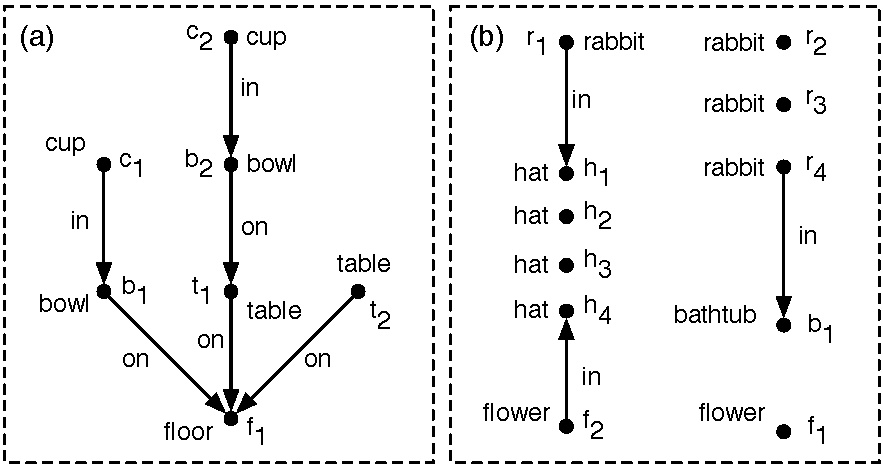
\includegraphics[width=8.5cm]{figures/pic-dale-haddock.pdf}\\[0pt]
\caption{}
\label{fig:dale-haddock}
\end{center}
\end{figure}


Cada f\'ormula de una descripci\'on l\'ogica denota un conjunto de objetos del dominio; por lo tanto podemos usar tales f\'ormulas para describir conjuntos. Por ejemplo en el modelo de la Figura.~\ref{fig:dale-haddock}b, la f\'ormula
$\mathsf{flower}$ denota el conjunto $\{f_1,f_2\}$; La f\'ormula
$\mathsf{flower} \sqcap \exists \mathsf{in}.\mathsf{hat}$ denota
$\{f_2\}$; y la f\'ormula $\mathsf{flower} \sqcap \neg
\exists \mathsf{in}.\mathsf{hat}$ denota $\{f_1\}$.\\

\textcolor{blue}{no se si dejar este ejemplo, o cambiarlo por uno es espa\~nol}

Hay muchas otras l\'ogicas de descripci\'on (DL) en la literatura por ejemplo 

$\mathcal{CL}$ (\el\ sin el cuantificador existencial, es decir solo conjunciones at\'omicas); $\mathcal{PL}$ (\alc\ l\'ogica propocisional); y
$\mathcal{ELU}_{(\neg)}$ (\el\ m\'as disjunci\'on y negaci\'on at\'omica).\\

Usaremos una noci\'on de preservaci\'on de f\'ormulas que llamaremos
\emph{similaridad}. Para cualquier DL $\gL$, diremos que un individual $i$ es \emph{\gL-similar} a $i'$ en un modelo dado $\gM$
si para cualquier f\'ormula $\varphi \in \gL$ tal que $i \in
\interp{\varphi}$, tambi\'en tenemos que $i' \in \interp{\varphi}$.\\
Equivalentemente, no hay $\gL$-f\'ormula que se mantenga para $i$ pero no para
$i'$.  Diremos que el \emph{\gL-conjunto de similaridad} de alg\'un individual
$i$ es el conjunto de todos los individuales a los cuales $i$ es \gL-similar.\\

Notar que la similaridad no es necesariamente una relaci\'on sim\'etrica: Por ejemplo:$f_1$ es \el-similar a $f_2$ en
Figura~\ref{fig:dale-haddock}b, pero $f_2$ no es \el-similar a $f_1$
(satisface la f\'ormula $\exists \mathsf{in}.\mathsf{hat}$ y $f_1$
no la satisface).  De todas maneras, \alc-similaridad es una relaci\'on sim\'etrica porque
el languaje contiene negaci\'on; y en consecuencia, $f_1$ no es \alc-similar
a $f_2$ porque este tampoco satisface $\neg \exists
\mathsf{in}.\mathsf{hat}$.  Porque \alc\ es m\'as expresivo que \el,
esto es, para alg\'un individual $a$ es posible ser \el-similar pero
no \alc-similar a alg\'un individual $b$, pero no viceversa.\\



%\textcolor{blue}{SACAR ESTO... poner quizas en la introduccion o en primer capitulo. Las ER que involucran relaciones han recibido m\'as atenci\'on recientemente;
%especialmente en el contexto de las expresiones referenciales espaciales en generaci\'on (por ejemplo,~\cite{kelleher06:increm}), donde es particularmente natural utilizar expresiones que implican relaciones espaciales, tales como ``la pelota en la parte superior del cubo''. Sin embargo, el algoritmo cl\'asico por~\cite{dale91:gener} ha demostrado ser incapaz de generar ER satisfactorias en la pr\'actica (v\'ease el an\'alisis sobre el~\emph{cabinet corpus} en~\cite{viethen06:_algor_for_gener_refer_expres}). Adem\'as, el Dale y Haddock algoritmo y muchos de sus sucesores (tales como~\cite{kelleher06:increm}) son vulnerables a el problema de la \emph{regresi\'on infinita}, donde el algoritmo entra en un bucle infinito, saltando hacia atr\'as y hacia adelante entre las descripciones para dos individuos emparentados, como en `` el libro sobre la mesa que soporta una libro sobre la mesa \ldots ''}

%REs involving relations have received increasing attention recently;
%especially in the context of spatial referring expressions in situated
%generation (e.g., \cite{kelleher06:increm}),
%where it is particularly natural to use expressions involving spatial
%relations such as ``the ball on top of the cube.''  However, the
%classical algorithm
%by~\cite{dale91:gener} was shown to be
%unable to generate satisfying REs in practice (see the analysis over
%the \emph{cabinet corpus}
%in~\cite{viethen06:_algor_for_gener_refer_expres}).  Furthermore, the
%Dale and Haddock algorithm and many of its successors (such
%as~\cite{kelleher06:increm}) are vulnerable to
%the problem of \emph{infinite regress}, where the algorithm enters an
%infinite loop, jumping back and forth between descriptions for two
%related individuals, as in ``the book on the table which supports a
%book on the table \ldots''

%\cite{arec2:2008:Areces,arec:usin11} have proposed low complexity
%algorithms for the generation of relational REs
%%(including references to sets) 
%that eliminate the risk of infinite regression.  These algorithms are
%based on variations of the partition refinement algorithms
%of~\cite{paig:thre87}.  The information provided by a given scene
%is interpreted as a relational model whose objects are classified into
%sets that fit the same description.  This classification is
%successively \emph{refined} till the target is the only element
%fitting the description of its class.  The existence of an ER depends
%on the information available in the input scene, and on the expressive
%power of the formal language used to describe elements of the
%different classes in the refinement.


\cite{arec2:2008:Areces,arec:usin11} han propuesto algoritmos de baja complejidad
 para la generaci\'on de ER relacionales que eliminan el riesgo de regresi\'on infinita. Estos algoritmos son
basados en variaciones de los algoritmos de refinamiento de particiones
de~\cite{paig:thre87}. La informaci\'on proporcionada por una escena dada
se interpreta como un modelo relacional cuyos objetos se clasifican en
conjuntos que se adaptan a la misma descripci\'on. Esta clasificaci\'on es
sucesivamente \emph{refinada} hasta que el target es el \'unico elemento
en la clase. La existencia de una ER depende
de la informaci\'on disponible en la escena de entrada, y del poder expresivo
del lenguaje formal utilizado para describir los elementos de las
diferentes clases en el refinamiento.\\

%Refinement
%algorithms %presented in~\cite{arec2:2008:Areces,arec:usin11}
%effectively compute REs for all individuals in the domain, at the same
%time. The algorithms always terminate returning a formula of the
%formal language chosen that uniquely describes the target (if the
%formal language is expressive enough to identify the target in the
%input model).
%\cite{arec2:2008:Areces}
%show that the refinement algorithm using the description language \el  is capable of generating 67\% of 
%the relational REs in the~\cite{viethen06:_algor_for_gener_refer_expres} dataset, when all possible orders of the relations in the domain are considered. This is in sharp contrast with the analysis 
%done in~\cite{viethen06:_algor_for_gener_refer_expres} over the cabinet corpus, of algorithms based in Dale and Reiter's original proposal.    

%Los algoritmos de refinamiento
% presenta en~\cite{arec 2:2008:Areces, arec:usin11}
%calculan efectivamente ER para todos los objetos en el dominio, al mismo
%tiempo. Los algoritmos siempre terminan devolviendo una f\'ormula del
%lenguaje formal elegido que describe un\'{i}vocamente el target (si el
%lenguaje formal es suficientemente expresivo para identificar el target en el
%modelo de entrada).\\

%Refinement algorithms for GER are based on the following basic idea:
%given a scene $S$, the objects appearing in $S$ are successively
%classified according to their properties into finer and finer
%classes. A description (in some formal language $\mathcal{L}$) of each
%class is computed every time a class is refined. The procedure always
%stops when the set of classes stabilizes, i.e., no further refinement
%is possible with the information available in the scene\footnote{Of
%  course, if we are only interested in a referring expression for a
%  given target we can stop the procedure as soon as the target is the
%  only element of some of the classes.}.  If the target element is in
%a singleton class, then the formal description of that class is a
%referring expression; otherwise the target cannot be unequivocally
%described (in 


%It is clear that a scene can be encoded in different ways as a
%relational model (for example in \ref{figure22}, we could argue that
%$e_1$ is also \emph{leftof} $e_2$, not considered because they are no
%touching). The algorithm assumes that these issues have been resolved
%and that the model encodes a suitable representation of the scene we
%want to describe.  Moreover, we will assume that all relations are
%\emph{binary}.  We will not consider relations of arity greater than
%two (relations of higher arity can be encoded as binary relations via
%reification, if necessary).

\begin{figure}[ht]
%\begin{minipage}[b]{0.45\linewidth}
%\centering
\begin{center}
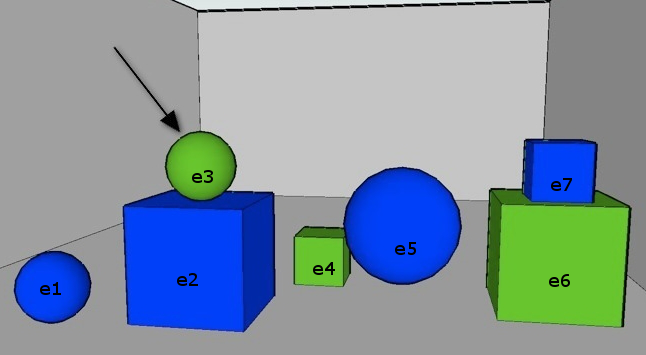
\includegraphics[width=0.5\textwidth]{images/3b.png}
\caption{Contexto de ejemplo}\label{GRE3D7-stimulus-cap2}
%\end{minipage}
\end{center}
\end{figure}

%\textcolor{blue}{hice mas grande la figura porque no se leian, como la pase a espaniol y se me fue al pie, no se porque}
%\hspace*{-0.35cm}
\begin{figure}[ht]
\begin{center}
%\begin{minipage}[b]{0.5\linewidth}
%\centering
\begin{tikzpicture}
  [
    n/.style={circle,fill,draw,inner sep=3pt,node distance=2.6cm},
    aArrow/.style={->, >=stealth, semithick, shorten <= 2pt, shorten >= 2pt},
  ]
 \node[n,label=above:$e_1$,label=below:{
    \relsize{-1}$\begin{array}{c}
      \nLeft\\[-2pt]
      \nSmall\\[-2pt] 
      \nBlue \\[-2pt] 
      \nBall\end{array}$}] (a) {};

 \node[n,label=above:$e_2$,label=below:{
    \relsize{-1}$\begin{array}{c}
      \nLeft\\[-2pt]
      \nBig\\[-2pt] 
      \nBlue\\[-2pt] 
      \nCube\end{array}$}, right of=a] (b) {};

 \node[n,label=below:$e_3$,label=above:{
    \relsize{-1}$\begin{array}{c}
      \nTop\\[-2pt]
      \nLeft\\[-2pt]
      \nSmall\\[-2pt] 
      \nGreen\\[-2pt] 
      \nBall\end{array}$}, above of=b] (c) {};

 \node[n,label=above:$e_4$,label=below:{
    \relsize{-1}$\begin{array}{c}
      \nSmall\\[-2pt] 
      \nGreen\\[-2pt] 
      \nCube\end{array}$}, right of=b] (d) {};

 \node[n,label=above:$e_5$,label=below:{
    \relsize{-1}$\begin{array}{c}
      \nBig\\[-2pt] 
      \nBlue\\[-2pt] 
      \nBall\end{array}$}, right of=d] (e) {};

 \node[n,label=above:$e_6$,label=below:{
    \relsize{-1}$\begin{array}{c}
      \nBig\\[-2pt] 
      \nGreen\\[-2pt] 
      \nCube\end{array}$}, right of=e] (f) {};

 \node[n,label=below:$e_7$,label=above:{
    \relsize{-1}$\begin{array}{c}
      \nTop\\[-2pt]
      \nSmall\\[-2pt] 
      \nBlue\\[-2pt] 
      \nCube\end{array}$}, above of=f] (g) {};

 \draw [aArrow,bend right=90] (b) to node[auto,swap]{\relsize{-1}$\nBelow$} (c);
 \draw [aArrow,bend right=90] (c) to node[auto,swap]{\relsize{-1}$\nOntop$} (b);

 \draw [aArrow,bend right=70] (d) to node[auto,swap]{\relsize{-1}$\nLeftof$} (e);
 \draw [aArrow,bend right=70] (e) to node[auto,swap]{\relsize{-1}$\nRightof$} (d);

 \draw [aArrow,bend right=90] (f) to node[auto,swap]{\relsize{-1}$\nBelow$} (g);
 \draw [aArrow,bend right=90] (g) to node[auto,swap]{\relsize{-1}$\nOntop$} (f);

 \draw[dotted] (-.6,-1.4) rectangle (12.5,4.5);

 \end{tikzpicture}
\caption{Modelo relacional del Contexto \ref{GRE3D7-stimulus-cap2}}
\label{GRE3D7-stimulus-graph}
%\end{minipage}
\end{center}
\end{figure}

Algoritmos de refinamiento para GER se basan en la siguiente idea b\'asica:
dada una escena $S$, los objetos que aparecen en $S$ son sucesivamente
clasificados de acuerdo con sus propiedades en clases m\'as y m\'as finas. 
Una descripci\'on (en alg\'un lenguaje formal de $\mathcal{L}$) de cada
clase se calcula cada vez que una clase es refinada. El procedimiento siempre
se detiene cuando el conjunto de clases se estabiliza, es decir, no se puede hacer m\'as refinamiento
con la informaci\'on disponible en la escena \footnote{Por supuesto, si s\'olo estamos interesados en una expresi\'on referencial de un objeto dado, se puede detener el procedimiento en cuanto el objetivo es el
   \'unico elemento de alguna de las clases.}

Si el elemento target est\'a en
una clase singleton, entonces la descripci\'on formal de esa clase es un
expresi\'on referencial; de lo contrario el target no puede ser un\'{i}vocamente
descripto (en $\mathcal{L}$).\\

Est\'a claro que una escena puede ser codificada en diferentes formas como un
modelo relacional (por ejemplo, en \ref{GRE3D7-stimulus-cap2}, podr\'{i}amos argumentar que
$e_1$ es tambi\'en \emph{leftof} $e_2$, pero no lo consideramos porque no se estan 
tocando en la imagen). El algoritmo asume que estas cuestiones se han resuelto y que el modelo codifica una representaci\'on adecuada de la escena que
queremos describir. Por otra parte, vamos a suponer que todas las relaciones son
\emph{binarias}. No vamos a considerar las relaciones de aridad mayor que
dos (relaciones de mayor aridad pueden codificarse como relaciones binarias v\'{i}a
reificaci\'on, si es necesario).\\

%On termination, the algorithm computes what are called the
%$\mathcal{L}$-similarity classes of the input model $\gM$.
%Intuitively, the referring expression ``\textsf{ball}'' and ``\textsf{cube}''  are more specific and then contain more information than $\top$.


Tras la resoluci\'on, el algoritmo calcula lo que se llama la
$\mathcal{L}$ - clases de semejanza del modelo de entrada de $\gM$.\\

%There is many $\mathcal{L}$, we will name $\alc$ and $\el$

%ACA VOY A PONER gramatica para generar... ALC y EL no quedaria bien aca, hay que ver lo agregamos antes o no hace falta
%In what follows, we use formulas of the $\el$ description logic
%language
En lo que sigue, se utilizan f\'ormulas de la descripci\'on de la l\'ogica $\el$
~\cite{baad:desc03} para describir las clases de refinamiendo
\footnote{N\'otese, sin embargo, que el lenguaje formal particular usado es
   independiente del algoritmo principal, y diferentes funciones
  add$_{\mathcal{L}}$($\varphi$,\RE) se pueden utilizar dependiendo
   de la l\'ogica en cuesti\'on.}. como se discuti\'o 
en~\cite{arec2:2008:Areces}, 
este lenguaje es adecuado para describir
RE conjuntivas y relacionales, que son lo que encontramos en los corpus.

  La entrada al algoritmo ser\'a un modelo $\mathcal{M} =
 \tup{\Delta, \interp{\cdot}}$, donde $\Delta$ es el dominio no vac\'io de objetos de la imagen,
 $\interp{\cdot}$ es una funci\'on de interpretaci\'on que asigna a todas las propiedades de la escena su extensi\'on.
 Por ejemplo, la escena mostrada en la Figura~\ref{GRE3D7-stimulus-cap2} podr\'ia ser representada por el modelo
 $\gM=\tup{\Delta,\interp{\cdot}}$ mostrado en la 
 Figura~\ref{GRE3D7-stimulus-graph}; donde+- $\Delta =
 \{e_1,\ldots,e_7\}$, e $\interp{\textsf{red}}$ is $\{e_2, e_4, e_5,
 e_7\}$.

Se llama extensi\'on de una f\'ormula al conjunto de objetos que la hacen v\'alida.

$\top$ es una f\'ormula que representa la descripci\'on m\'as general, cuya
interpretaci\'on incluye todos los elementos del modelo. Se podr\'ia realizar
como la ER con el sustantivo
``\textsf{cosa}''. Decimos que una f\'ormula es
\emph{subsumida} por otras f\'ormulas, cuando su extensi\'on puede ser cubierta por la
union de las extensiones de las otras f\'ormulas. Por ejemplo, en la
Figura~\ref{GRE3D7-stimulus-cap2}, $\top$ es subsumida por ``\textsf{ball}'' y
``\textsf{cube}'', porque $\interp{\top}$ = $\interp{\textsf{ball}}
\cup \interp{\textsf{cube}}$.
%= $\{e_2, e_4, e_6, e_7\}$, it is $\{e_1, e_2, e_3, e_4, e_5, e_6, e_7\}$ = $\{e_1, e_3, e_5\} \cup \{e_2, e_4, e_6, e_7\}$. 
Intuitivamente la f\'ormula ``\textsf{cube}'' o ``\textsf{ball}'' tienen m\'as informaci\'on que $\top$, para cada elemento de $\top$, hay una f\'ormula que d\'a m\'as informaci\'on, digamos ``\textsf{cube}'' es m\'as informativa que ``\textsf{cosa}''.\\

%In the following we will explain an example of execusion of the
%algorithm shown in Figure
%A continuaci\'on vamos a explicar un ejemplo de ejecusi\'on del
%algoritmo mostrado en la Figura~\ref{algoritmoOriginal} considerando la l\'ogica 
%$\el$ como language. Este algoritmo fue presentado en
%~\cite{arec2:2008:Areces}.
%
%\begin{figure}[h!]
%\begin{center}
%\includegraphics[width=\textwidth]{images/algoritmoOriginal.png}
%\end{center}
%\vspace*{-2em}
%\caption{Algoritmo para GER con l\'ogicas de descripci\'on}
%\label{algoritmoOriginal}
%\end{figure}

%\subsection{Ejemplo de ejecuci\'on}
%
%
%
%\textcolor{blue}{no se si poner aca un ejemplo, si poner el texto y las im\'agenes en otro apendice... o ponerlas mas chiquitas en varias columnas, asi queda feo}\\
%Vamos a ejecutar el algoritmo para la Figura~\ref{GRE3D7-stimulus-cap2},
%el algoritmo comienza con una lista fija de propiedades y relaciones, supongamos que
%esas listas son las siguientes:
%
%propiedades ordenadas (prop): \textsf{ball}, \textsf{cube}, \textsf{red}, \textsf{yellow}, \textsf{small}, \textsf{large}.\\
%relaciones ordenadas (rel): \textsf{leftof}, \textsf{rightof}, \textsf{ontopof}, \textsf{bellowof}.
%
%%\begin{figure}
%%\begin{center}	
%%\includegraphics[width=.5\textwidth]{images/22.jpg}
%%\end{center}
%%\vspace*{-1.5em}
%%\caption{Escena 3D de figuras geom\'etricas}\label{figure22}
%%\end{figure}
%
%%\begin{figure}
%%\begin{minipage}[b]{0.6\linewidth}
%%\centering
%%\begin{tikzpicture}
%%  [
%%    n/.style={circle,fill,draw,inner sep=3pt,node distance=1.4cm},
%%    aArrow/.style={->, >=stealth, semithick, shorten <= 2pt, shorten >= 2pt},
%%  ]
%% \node[n,label=above:$e_1$,label=below:{
%%    \relsize{-1}$\begin{array}{c}
%%      \nLeft\\[-2pt]
%%      \nSmall\\[-2pt] 
%%      \nYellow \\[-2pt] 
%%      \nBall\end{array}$}] (a) {};
%
%% \node[n,label=above:$e_2$,label=below:{
%%    \relsize{-1}$\begin{array}{c}
%%      \nLeft\\[-2pt]
%%      \nSmall\\[-2pt] 
%%      \nRed\\[-2pt] 
%%      \nCube\end{array}$}, right of=a] (b) {};
%
%% \node[n,label=below:$e_3$,label=above:{
%%    \relsize{-1}$\begin{array}{c}
%%      \nTop\\[-2pt]
%%      \nLeft\\[-2pt]
%%      \nSmall\\[-2pt] 
%%      \nYellow\\[-2pt] 
%%      \nBall\end{array}$}, above of=b] (c) {};
%
%% \node[n,label=above:$e_4$,label=below:{
%%    \relsize{-1}$\begin{array}{c}
%%      \nBig\\[-2pt] 
%%      \nRed\\[-2pt] 
%%      \nCube\end{array}$}, right of=b] (d) {};
%
%% \node[n,label=above:$e_5$,label=below:{
%%    \relsize{-1}$\begin{array}{c}
%%      \nBig\\[-2pt] 
%%      \nRed\\[-2pt] 
%%      \nBall\end{array}$}, right of=d] (e) {};
%
%% \node[n,label=above:$e_6$,label=below:{
%%    \relsize{-1}$\begin{array}{c}
%%      \nSmall\\[-2pt] 
%%      \nYellow\\[-2pt] 
%%      \nCube\end{array}$}, right of=e] (f) {};
%
%% \node[n,label=above:$e_7$,label=below:{
%%    \relsize{-1}$\begin{array}{c}
%%      \nSmall\\[-2pt] 
%%      \nRed\\[-2pt] 
%%      \nCube\end{array}$}, right of=f] (g) {};
%
%% \draw [aArrow,bend right=90] (b) to node[auto,swap]{\relsize{-1}$\nBelow$} (c);
%% \draw [aArrow,bend right=90] (c) to node[auto,swap]{\relsize{-1}$\nOntop$} (b);
%
%% \draw [aArrow,bend right=30] (d) to node[auto,swap]{\relsize{-1}$\nLeftof$} (e);
%% \draw [aArrow,bend right=30] (e) to node[auto,swap]{\relsize{-1}$\nRightof$} (d);
%
%% \draw [aArrow,bend right=30] (f) to node[auto,swap]{\relsize{-1}$\nLeftof$} (g);
%% \draw [aArrow,bend right=30] (g) to node[auto,swap]{\relsize{-1}$\nRightof$} (f);
%
%% \draw[dotted] (-.4,-1.7) rectangle (7.5,3.3);
%
%% \end{tikzpicture}
%%\caption{La escena como modelo relacional}\label{GRE3D7-stimulus-graph}
%%\end{minipage}
%%\end{figure}
%
%
%El algoritmo siempre termina, y devuelve ER un conjunto de f\'ormulas que describe cada elemento en el dominio (si existe esa f\'ormula). \\
%
%En el comienzo ER=$\{\top\}$ y $\interp{\top}$ = $\{e_1, e_2, e_3, e_4, e_5, e_6, e_7\}$ como se puede ver en la Figura~\ref{fig-modelo}.\\
%
%ACA
%\begin{figure}[ht]
%\begin{minipage}[b]{0.45\linewidth}
%\centering
%\includegraphics[width=\textwidth]{images/22.jpg}
%\vspace*{1cm}
%%\caption{Input scene}
%\label{GRE3D7-stimulus-22}
%\end{minipage}
%%\hspace*{-0.35cm}
%\begin{minipage}[b]{0.6\linewidth}
%\centering
%%\begin{figure}[ht]
%%\begin{center}
%\frame{\includegraphics[width=8cm]{images/modelo.png}}\\[0pt]
%\caption{Modelo de la Figura \ref{GRE3D7-stimulus-22}}
%\label{fig-modelo}
%\end{minipage}
%\end{figure}
%El primer bucle del algoritmo es en las propiedades. Para cada propiedad hace add$_\el$ ($\varphi$, RE), las propiedades at\'omicas se muestran en la Figura~\ref{fig-modelo2}.
%
%\begin{figure}[ht]
%\begin{center}
%\frame{\includegraphics[width=8cm]{images/modelo2.png}}\\[0pt]
%\caption{Propiedades proposicionales en cuadro rojo, las del primer ciclo del algoritmo}
%\label{fig-modelo2}
%\end{center}
%\end{figure}
%
%La f\'ormula $\varphi$ se a\~nadir\'a a ER si su interpretaci\'on tiene al menos un elemento, a continuaci\'on, para cada f\'ormula
 %$\psi$ en ER la conjunci\'on
%$\varphi  \wedge \psi$ no necesita estar subsumida in ER, la $\interp{\varphi \cup \psi}$ no tiene que ser vac\'io, y su interpretaci\'on tiene que ser distinta de $\interp{\psi}$. Luego las f\'ormulas subsumidas se borran.
%
%La primer propiedad es \textsf{ball}, ER = \{$\top$, \textsf{ball}\}, se ven los elementos de ``ball'' en un recuadro en la Figura~\ref{fig-modelo3}.
%
%\begin{figure}[ht]
%\begin{center}
%\frame{\includegraphics[width=8cm]{images/modelo3.png}}\\[0pt]
%\caption{El cuadro indica cuales son ``ball''}
%\label{fig-modelo3}
%\end{center}
%\end{figure}
%
%La siguiente propiedad es \textsf{cube}, ER = \{$\top$, \textsf{ball}, \textsf{cube}\}, pero ahora la $\interp{\textsf{ball}}$ = $\{e_1, e_3, e_5\}$, $\interp{\textsf{cube}}$ = $\{e_2, e_4, e_6, e_7\}$, quedando las particiones como se muestra en la Figura~\ref{fig-modelo4}
%\begin{figure}[ht]
%\begin{center}
%\frame{\includegraphics[width=8cm]{images/modelo4.png}}\\[0pt]
%\caption{Cuadros indicando ``ball'' y ``cube''}
%\label{fig-modelo4}
%\end{center}
%\end{figure}
%Ahora podemos borrar $\top$, porque es subsumida (esta cubierta por) las otras dos f\'ormulas. La siguiente propiedad es  \textsf{red}, $\interp{\textsf{red}}$ es: $\{e_2, e_4, e_5, e_7\}$, haciendo la intersecci\'on con la $\interp{.}$ de cada f\'ormula en ER obtenemos, $\{e_5\}$ y $\{e_2, e_4, e_7\}$, ER = $\{\textsf{ball}, \textsf{cube}, \textsf{ball} \wedge \textsf{red}, \textsf{cube} \wedge \textsf{red}\}$, las particiones actuales se pueden ver en la Figura~\ref{fig-modelo9}.
%\begin{figure}[ht]
%\begin{center}
%\frame{\includegraphics[width=8cm]{images/modelo9.png}}\\[0pt]
%\caption{Cuadros indicando ``ball'', ``cube'' y ``red''}
%\label{fig-modelo9}
%\end{center}
%\end{figure}
%
%Siguiendo con \textsf{yellow}, tenemos, $\interp{\textsf{yellow}}$ = $\{e_1, e_3, e_6\}$ y obtenemos ER = $\{\textsf{ball} \wedge \textsf{yellow}, \textsf{cube} \wedge \textsf{yellow}, \textsf{ball} \wedge \textsf{red}, \textsf{cube} \wedge \textsf{red}\}$. 
%Note que aqu\'i ya borramos la f\'ormula \textsf{ball} porque estaba subsumida, y la f\'ormula \textsf{cube} tambi\'en. Se muestran particiones en Figura~\ref{fig-modelo10}.
%
%\begin{figure}[ht]
%\begin{center}
%\frame{\includegraphics[width=8cm]{images/modelo10.png}}\\[0pt]
%\caption{Cuadros indicando ``ball'', ``cube'', ``red'' y ``yellow''}
%\label{fig-modelo10}
%\end{center}
%\end{figure}
%
%Haciendo lo mismo con \textsf{small} tenemos ER = $\{\textsf{ball} \wedge \textsf{yellow} \wedge \textsf{small}, \textsf{cube} \wedge \textsf{yellow} \wedge \textsf{small}, \textsf{ball} \wedge \textsf{red}, \textsf{cube} \wedge \textsf{red}, \textsf{cube} \wedge \textsf{red} \wedge \textsf{small}\}$, como se puede ver en Figura~\ref{fig-modelo11}.
%\begin{figure}[ht]
%\begin{center}
%\frame{\includegraphics[width=8cm]{images/modelo11.png}}\\[0pt]
%\caption{Cuadros indicando ``ball'', ``cube'', ``red'', ``yellow'', ``small'' y ``large''}
%\label{fig-modelo11}
%\end{center}
%\end{figure}
%
%La siguiente propiedad es \textsf{large} as\'i, tenemos ER = $\{\textsf{ball} \wedge \textsf{yellow} \wedge \textsf{small}, \textsf{cube} \wedge \textsf{yellow} \wedge \textsf{small}, \textsf{ball} \wedge \textsf{red}, \textsf{cube} \wedge \textsf{red} \wedge \textsf{large}, \textsf{cube} \wedge \textsf{red} \wedge \textsf{small}\}$. Aqu\'i no podemos agregar \textsf{large} a la f\'ormula $\textsf{red} \wedge \textsf{cube}$ porque su interpretaci\'on tiene un solo elemento, y la condici\'on dice que es necesario tener m\'as de uno.
%
%Hasta ahora ER = $\{\textsf{ball} \wedge \textsf{yellow} \wedge \textsf{small}, \textsf{cube} \wedge \textsf{yellow} \wedge \textsf{small}, \textsf{ball} \wedge \textsf{red}, \textsf{cube} \wedge \textsf{red} \wedge \textsf{large}, \textsf{cube} \wedge \textsf{red} \wedge \textsf{small}\}$ 
%y tenemos las siguientes extensiones: $\{e_1, e_3\}, \{e_6\}, \{e_5\}, \{e_4\}, \{e_2, e_7\}$ respectivamente. 
%Hay dos f\'ormulas que a\'un pueden ser refinadas, $\textsf{ball} \wedge \textsf{yellow} \wedge \textsf{small}$ y $\textsf{cube} \wedge \textsf{red} \wedge \textsf{small}$ 
%debido a que tienen m\'as de un elemento cada una, por lo que entran en el ciclo, while del algoritmo 1, en la l\'inea 4. Ahora es el turno de las relaciones, la primera de ellas es \textsf{leftof}, para cada f\'ormula $\varphi$ en ER trataremos de hacer add$_\el$ ($\exists \textsf{leftof}.\varphi$, RE). Notar que $\psi$ solo puede ser $\textsf{ball} \wedge \textsf{yellow} \wedge \textsf{small}$ o $\textsf{cube} \wedge \textsf{red} \wedge \textsf{small}$ porque esos son los que su interpretaci\'on tiene m\'as de un elemento. 
%\begin{figure}[ht]
%\begin{center}
%\frame{\includegraphics[width=8cm]{images/modelo15.png}}\\[0pt]
%\caption{Cuadros indicando ``ball'', ``cube'', ``red'', ``yellow''...}
%\label{fig-modelo15}
%\end{center}
%\end{figure}
%
%
%No hay
%%because those are the ones that its interpretation have more than one element. There is not 
%$\varphi$ y $\psi$ que puedan ser aplicadas. Continuando con \textsf{rightof} agregamos $\textsf{cube} \wedge \textsf{yellow} \wedge \textsf{small} \wedge \exists \textsf{rightof}. \textsf{cube} \wedge \textsf{red} \wedge \textsf{small}$, y asi con \textsf{topof} agregamos $\textsf{small} \wedge \textsf{red} \wedge \textsf{cube} \wedge \exists \textsf{ontop}. \textsf{small} \wedge \textsf{yellow} \wedge \textsf{ball}$ y el algoritmo termina con ER = $\{\textsf{ball} \wedge \textsf{yellow} \wedge \textsf{small}, \textsf{cube} \wedge \textsf{yellow} \wedge \textsf{small}, \textsf{ball} \wedge \textsf{red}, \textsf{cube} \wedge \textsf{red} \wedge \textsf{large}, \textsf{cube} \wedge \textsf{red} \wedge \textsf{small}, \textsf{cube} \wedge \textsf{yellow} \wedge \textsf{small} \wedge \exists \textsf{rightof}. \textsf{cube} \wedge \textsf{red} \wedge \textsf{small}, \textsf{small} \wedge \textsf{red} \wedge \textsf{cube} \wedge \exists \textsf{ontop}. \textsf{small} \wedge \textsf{yellow} \wedge \textsf{ball}\}$, 
%aqu\'i todos los elementos est\'an en una clase singleton y no se puede hacer ning\'un refinamiento m\'as. 
%%can be applied to $cube \wedge red \wedge small$ but there is no formula which interpretation has more than one element to be apply with this one. The same happen for the other relations, so the algorithm ends.
%%its interpretation is $\{e_7\}$ with $\psi$ is $cube \wedge yellow \wedge small$, the others combinations can't be apply because they don't do true the preconditions. The following relation is rightof, 
%
%%leftof, rightof, ontopof, bellowof
%
%%At this point we already have the target in a singleton set. So the formula for it is ``red and ball'', and also for s6 which formula is ``yellow cube''.\\
%%As we show this algorithm depends of the order of properties and relations.\\
%\begin{figure}[ht]
%\begin{center}
%\frame{\includegraphics[width=8cm]{images/modelo16.png}}\\[0pt]
%\caption{Cuadros indicando ``ball'', ``cube'', ``red'', ``yellow''...}
%\label{fig-modelo16}
%\end{center}
%\end{figure}
%
%\begin{figure}[ht]
%\begin{center}
%\frame{\includegraphics[width=8cm]{images/modelo17.png}}\\[0pt]
%\caption{Cuadros indicando ``ball'', ``cube'', ``red'', ``yellow''...}
%\label{fig-modelo17}
%\end{center}
%\end{figure}
%
%Las expresiones referenciales encontradas son:\\
%
%$\textsf{ball} \wedge \textsf{yellow} \wedge \textsf{small}$ representa $e_1$ \\
%$\textsf{cube} \wedge \textsf{yellow} \wedge \textsf{small}$ representa $e_6$ \\
%$\textsf{ball} \wedge \textsf{red}$ representa $e_5$ \\
%$\textsf{cube} \wedge \textsf{red} \wedge \textsf{large}$ representa $e_4$ \\
%$\textsf{cube} \wedge \textsf{red} \wedge \textsf{small}$ representa $\{e_2,e_7\}$  \\
%$\textsf{cube} \wedge \textsf{yellow} \wedge \textsf{small} \wedge \exists \textsf{rightof}. \textsf{cube} \wedge \textsf{red} \wedge \textsf{small}$ representa $e_6$ \\
%$\textsf{small} \wedge \textsf{red} \wedge \textsf{cube} \wedge \exists \textsf{ontop}. \textsf{small} \wedge \textsf{yellow} \wedge \textsf{ball}$ representa $e_2$ \\
%



\section{Aproximaciones emp\'iricas a la soluci\'on de GER}

\subsection{Corpus existente}
\label{sec:corpus2}
\label{sec:corpusTUNA}

%was the first prominent REG corpus to be made publicly available for research purposes. The corpus was developed in a series of general-purpose controlled experiments, containing 2280 descriptions produced by 60 speakers in two domains (1200 descriptions of furniture items and 1080 descriptions of people's photographs). TUNA does not contain relational descriptions, and it is possibly the only resource of this kind to include situations of reference to sets. The TUNA corpus has been extensively used in a series of shared tasks

TUNA \cite{tuna-corpus} fue el primer corpus prominente para GER disponible p\'ublicamente con fines de investigaci\'on. El corpus fue desarrollado en una serie de experimentos controlados de prop\'osito general, contiene 2.280 descripciones producidas por 60 personas en dos dominios (1.200 expresiones referenciales de im\'agenes de muebles y 1080 expresiones referenciales de fotograf\'ias de personas situadas en una grilla). Se muestran ejemplos de im\'agenes en Figuras \ref{fig-TUNA-furniture} y \ref{fig-TUNA-people}. El corpus TUNA no contiene descripciones relacionales, y es posiblemente el \'unico recurso de este tipo que incluye situaciones de referencia a conjuntos. Este corpus se ha utilizado ampliamente en una serie de desaf\'ios \cite{reg2009}. \\

\begin{figure}
\begin{minipage}[t]{0.5\linewidth}
\centering
\includegraphics[width=\textwidth]{images/largeGreyChair.jpg}\\[0pt]
\caption{Imagen del TUNA corpus (muebles)}
\label{fig-TUNA-furniture}
\vspace*{.1cm}
\end{minipage}
\hspace*{0cm}
\begin{minipage}[t]{0.5\linewidth}
\centering
\includegraphics[width=\textwidth]{images/tuna-people.jpg}\\[0pt]
\caption{Imagen del TUNA corpus (personas)}
\label{fig-TUNA-people}
\end{minipage}
\end{figure}


\label{sec:corpusGRE}
%were developed in a series of web-based experiments primarily focussed on the study of relational descriptions. GRE3D3 contains 630 descriptions produced by 63 speakers, and GRE3D7 contains 4480 descriptions produced by 287 speakers, making it the largest of its kind to date. The GRE3D domain consists of simple visual scenes containing only two kinds of objects (boxes and spheres) with limited variation in colour and size. In each scene, there is only one possible spatial relation between target and the nearest landmark. Both corpora contain atomic and relational descriptions.
GRE3D3 y su extensi\'on GRE3D7 \cite{gre3d3,gre3d7} se desarrollaron en una serie de experimentos basados en la web, se centraron principalmente en el estudio de las descripciones relacionales. GRE3D3 contiene 630 descripciones producidas por 63 personas y GRE3D7 contiene 4.480 descripciones producidas por 287 personas, y es el corpus m\'as grande de este tipo hasta la fecha. El dominio del GRE3D3 consta de escenas visuales simples que contienen s\'olo dos tipos de objetos (cubos y esferas) con variaci\'on limitada en color y tama\~no. En cada escena, s\'olo hay una posible relaci\'on espacial entre el target y el landmark m\'as cercano. Ambos corpus contienen descripciones at\'omicas y relacionales. Ejemplo de im\'agenes del GRE3D3 y GRE3D7 se muestran en las Figuras \ref{fig-GRE3D3} y \ref{fig-GRE3D7}.\\
%\begin{minipage}[b]{0.45\linewidth}

\begin{figure}
\begin{minipage}[b]{0.5\linewidth}
\centering
\includegraphics[width=\textwidth]{images/GRE3D3.png}\\[0pt]
\caption{Imagen del GRE3D3}
\label{fig-GRE3D3}
\vspace*{-0.7cm}
\end{minipage}
\hspace*{0cm}
\begin{minipage}[b]{0.5\linewidth}
\centering
\includegraphics[width=\textwidth]{images/3.jpg}\\[0pt]
\caption{Imagen del GRE3D7}
\label{fig-GRE3D7}
\end{minipage}
\end{figure}

%\vspace*{3cm}

\label{sec:corpusSTARS}
%and its extension Stars2 were collected for the study of referential overspecification (particularly in the case of relational descriptions). Stars was developed in a pilot web-based experiment, containing 704 descriptions produced by 64 speakers.  The more comprehensive Stars2 data set was produced in dialogue situations involving subject pairs, and it contains 884 descriptions produced by 56 speakers. Both domains make use of simple visual scenes containing up to four object types (e.g., stars, boxes, cones and spheres) with limited variation in colour and size. Differently from other REG corpora, however, Stars/2 includes a considerable number of complex situations of reference involving up to three objects, as in `the box near the sphere, next to the cone'.http://ppgsi.each.usp.br/arquivos/RelTec/PPgSI-002_2014.pdf y http://ppgsi.each.usp.br/arquivos/RelTec/PPgSI-001_2015.pdf
Stars \cite{stars-mutual-disamb} y su extensi\'on Stars2 se colectaron para el estudio de la sobre-especificaci\'on (particularmente en el caso de las descripciones relacionales). Stars se desarroll\'o en un experimento piloto basado en la web, contiene 704 descripciones producidas por 64 personas. El conjunto de datos Stars2 es m\'as completo y se obtuvo de situaciones de di\'alogo que implicaban a dos personas, contiene 884 descripciones producidas por 56 participantes. Ambos dominios hacen uso de escenas visuales simples que contienen tres tipos de objetos (por ejemplo para Stars, estrellas, cuadrados y c\'irculos y para Stars2 cubos, conos y esferas) con variaci\'on limitada en color y tama\~no. A diferencia de otros corpus para GER, Stars/2 incluyen un n\'umero considerable de situaciones complejas de referencia en que participan hasta tres objetos, como en ``el cubo cerca de la esfera, al lado del cono''. Ejemplos de imagenes se muestran en las Figuras \ref{fig-STARS} y \ref{fig-STARS2}.\\


\begin{figure}
\begin{minipage}[b]{0.5\linewidth}
\centering
\includegraphics[width=\textwidth]{images/STARS.png}\\[0pt]
\caption{Imagen de Stars corpus}
\label{fig-STARS}
%\vspace*{1cm}
\end{minipage}
\hspace*{0cm}
\begin{minipage}[b]{0.5\linewidth}
\centering
\includegraphics[width=\textwidth]{images/STARS2.png}\\[0pt]
\caption{Imagen de Stars2 corpus}
\label{fig-STARS2}
\end{minipage}
\end{figure}

%ejemplo minipage
%\begin{figure}
%\begin{minipage}[b]{0.5\linewidth}
%\centering
%\includegraphics[width=\textwidth]{figures/rest-singular2x.png}\\[0pt]
%\caption{Target singular con zoom 2X}
%\label{rest-singular2x}
%\end{minipage}
%\vspace*{.1cm}
%\begin{minipage}[b]{0.5\linewidth}
%\centering
%\includegraphics[width=\textwidth]{figures/rest-plural2x.png}\\[0pt]
%\caption{Target plural con zoom 2X}
%\label{rest-plural2x}
%\end{minipage}
%\end{figure}




%Despite their usefulness and general contribution to the research in REG, the above domains are still at a certain distance from the kinds of visual scene that might be required for a practical, real-world application. The need for additional complexity and/or realism, and our own interest in the surface realisation task for the Spanish and Portuguese languages, has led us to build a new computational resource of this kind. This work is described in the next sections. Further discussion on the differences between the Zoom corpus and existing resources is presented in Sec. \ref{sec-annotation}. 



\subsection{Trabajos emp\'iricos en el \'area}

%http://link.springer.com/chapter/10.1007/978-3-642-15573-4_9
%http://www.jetteviethen.net/papers/DaleViethen2010chapter.pdf

La investigaci\'on presentada en \cite{viethen-phd} se basa en dos premisas fundamentales: que la investigaci\'on
en la generaci\'on autom\'atica de expresiones referenciales debe esforzarse por lograr
sistemas que den salidas tan similar a la humana como sea posible; y que, para ello, debemos
esforzarnos para modelar el comportamiento humano como se puede observar en corpora.

La adopci\'on de estas premisas sirve para dos fines: en primer lugar, mejora la adecuaci\'on
de la salida de algoritmos de GER para el objeto target imitando la capacidad humana
de producir referencias adecuadas; y en segundo lugar, el estudio de corpus de datos producidos por humanos
 y algoritmos en desarrollo que pueden replicar estos datos podr\'ian
acercarnos a la comprensi\'on de que es lo que hacen los humanos cuando dan una ER.\\

Se\~nala que el cl\'asico algoritmo de GER y la mayor parte de sus descendientes no se basaron ni evaluaron contra datos producidos por humanos. Ellos se basaron en una visi\'on bastante minimalista de lo que se necesita
para que una expresi\'on referencial sea \'optima, concentr\'andose en la eficiencia computacional 
 y descripciones breves como sus principales preocupaciones.\\

 Existe un peque\~no n\'umero de enfoques que 
 se basaron en observaciones del comportamiento de referencia general humana
que obtuvieron a partir de experimentos psicoling\"u\'isticos, pero de nuevo no fueron evaluados
contra datos humanos.\\

Los algoritmos que se presentaron a los desaf\'ios de evaluaci\'on \cite{gatt-balz-kow:2008:ENLG} y \cite{reg2009}
fueron probados en el TUNA-Corpus, y algunos de ellos
tambi\'en tuvieron en cuenta los patrones que se encontraban en el conjunto del desarrollo. Pero hay una serie de preocupaciones en torno a la pregunta de si el TUNA-Corpus, y la forma de salida de los sistemas que se compar\'o 
en los desaf\'ios eran ideales para una evaluaci\'on de la adecuaci\'on descriptiva de GER.\\
%saque esto porque no se entiende
%A partir de los desaf\'ios que se describen en m\'as detalle y para evaluarlos en una serie de datos m\'as grande
%que contiene m\'as de una expresi\'on referencial para cada elemento est\'imulo.
Aborda tres \'areas principales en las que los corpus se puede utilizar para
promover el objetivo de la semejanza humana en la investigaci\'on sobre generaci\'on de expresiones referenciales:
evaluaci\'on, la recolecci\'on de corpus y an\'alisis y modelizaci\'on estad\'istica de
datos de corpus.\\
Comenz\'o con el an\'alisis del estado del arte de la investigaci\'on en
la generaci\'on de descripciones distintivas, trabaj\'o con relaciones espaciales y en el trabajo us\'o datos de corpus. Examin\'o una serie de opciones metodol\'ogicas que tienen que hacerse cuando se trabaja con los corpus de GER. Aqu\'i, explor\'o diferentes opciones para los desaf\'ios de recopilaci\'on de corpus, que se centran en torno al equilibrio que se necesita
entre el control de los par\'ametros experimentales tanto como sea necesario
y mantener la configuraci\'on de lo m\'as natural posible. Discuti\'o una serie de conceptos
que son de importancia para el an\'alisis de corpora de GER, tales como la naturalidad de diferentes
propiedades de los objetos, y las nociones de minimalidad y cuestiones de sobre-especificaci\'on de expresiones referenciales. Por \'ultimo, analiz\'o diferentes maneras en que la salida de un sistema se puede
comparar con los datos de corpora, bajo la premisa de que el objetivo de la comparaci\'on es
para evaluar si el sistema podr\'ia tener un modelo adecuado del comportamiento humano para la generaci\'on de expresiones referenciales.
Realiz\'o una investigaci\'on en las tres \'areas donde se puede emplear corpora en GER: Evaluaci\'on de semejanza humana, recopilaci\'on y an\'alisis de corpus, y modelado de datos de corpus. Realiz\'o un experimento de evaluaci\'on con tres de los algoritmos cl\'asicos, (1989) Algoritmo Greedy de Dale (Greedy), Dale y Haddock (1991b), Algoritmo Relacional (ra) Y Dale y Reiter (1995) Algoritmo Incremental (IA), Se pusieron a prueba en cuanto a su capacidad de
replicar las expresiones referenciales se encuentran en un grupo relativamente peque\~no de corpus de expresiones referenciales
en un dominio visual de im\'agenes puestas en una grilla.
%de rejilla de cajones de armarios ling. 
En el an\'alisis de este experimento tuvo dos resultados principales: (1) que identic\'o en particular tres 
fen\'omenos que todav\'ia plantean importantes retos para los algoritmos GER con el objetivo de replicar
el comportamiento humano, y (2) que proporciona una plataforma para la discusi\'on de una serie de
dificultades que se presentan para la evaluaci\'on basada en corpus de GER. Esto result\'o en una serie
de criterios para el dise\~no de los dos corpus que el trabajo en el resto de la tesis.
Los tres fen\'omenos en las expresiones referenciales producidas por humanos que los
algoritmos probados no fueron capaces de replicar satisfactoriamente sobre-especificaci\'on,
relaciones espaciales, y comportamiento de voluntarios espec\'ificos. Ambos
Greddy y la IA fueron capaces de generar algo de la redundancia que se encontr\'o en el corpus.
 Ni Greedy ni el IA estaban dise\~nados para ser capaz de generar expresiones referenciales que contengan relaciones entre entidades, pero el ra fue dise\~nado para incluirlas. Sorprendentemente, el
ra no s\'olo fallo en generar cualquiera de las descripciones contenidas en el corpus de evaluaci\'on; sino tambi\'en que las descripciones que se gener\'o parec\'ian m\'as como enigmas cuyo objetivo era confundir a un oyente, m\'as que ayudar en
los intentos de se\~nalar el objetivo referente. 

Una valoraci\'on te\'orica de otras aproximaciones dise\~nados para manejar las relaciones estableci\'o que ninguno de ellos incluir\'ia una relaci\'on, si no es absolutamente necesaria para distinguir el target.
La tercera observaci\'on que el experimento dejo a la vista fue que la gente no siempre hace lo mismo en la misma situaci\'on. De hecho, incluso la misma persona podr\'ia describir el mismo target de diferente manera en distintas
circunstancias. 

 None of the algorithms tested were intended to take such inter- and
intra-speaker variation into account, and only very recently have implementations
of the
ia
begun to model speaker-preferences to some degree.

No se pretend\'ia que ninguno de los algoritmos de la prueba tomara en cuenta las variaciones entre-hablantes, ni del mismo hablante. Hay implementaciones del IA que han comenzado a agregar modelo de preferencias de hablante en alg\'un grado.

Los temas generales con evaluaci\'on basada en corpus que esta experiencia de evaluaci\'on dej\'o
al descubierto fueron (1) la interdependencia estrecha entre algoritmos y la
representaci\'on subyacente de conocimiento que utilizan, (2) el no-determinismo de la generaci\'on del lenguaje natural, (3) la cuesti\'on de c\'omo comparar la salida algoritmos con gold-standar, y (4) el dominio espec\'ifico de los algoritmos de GER.\\
La discusi\'on de estos temas ha dado lugar a la siguiente lista de Evaluaci\'on en GER basado en corpus:

1. Si el corpora est\'a destinado para ser reutilizado para la evaluaci\'on comparativa de diferentes
algoritmos, una representaci\'on subyacente del dominio debe ser proporcionada para ser usada por todos los algoritmos.

2. Si queremos confiar en los resultados, el corpus debe contener tantos casos como sea posible de tantos direntes hablantes como sea posible para cada escenario referencial. 
Esto es cierto si un algoritmo es evaluado en t\'erminos de ser capaz de generar una expresi\'on referencial que suene natural, o si est\'a probado por su probabilidad de pertenecer a un modelo espec\'ifico de conducta humana de referencia, mediante la comprobaci\'on de si se puede generar todas las descripciones en un corpus.

3. Si la probabilidad de un algoritmo de ser un modelo de la conducta humana de referencia
se eval\'ua, deben utilizarse m\'etricas basadas en recuento (RECALL) y precisi\'on (PRESITION). En este
caso, el conjunto completo de las descripciones que el algoritmo proporciona para cada
escenario de referencia en virtud de cualquier ajuste de par\'ametro debe ser comparado con el
conjunto de las descripciones contenidas en el corpus para el mismo escenario referencial.
Si la capacidad m\'as orientada a la aplicaci\'on para generar una referencia es similar a la humana
se ha de evaluar, s\'olo una descripci\'on por escenario.
Esto debe hacerse utilizando m\'etricas basadas en la precisi\'on para probar c\'omo muchos de las
descripciones dadas por los algoritmos est\'an contenidas en el corpus.
4. Algoritmos que son juzgados en un dominio espec\'ifico c, no se debe asumir como
f\'acilmente adaptable a otros dominios. Idealmente, los corpus que abarcan muchos diferentes
deben estar disponibles para las pruebas de los algoritmos que generalizan en distintos tipos de dominios.
Realiz\'o 2 corpus el GRE3D3 y el GRE3D7 descriptos en \ref{sec:corpus2}

Trabaj\'o con \'arboles de decisi\'on ...
\textcolor{blue}{Aca agregar otras personas que usaron corpus para generacion de ER, Ivandre... }

%http://www.lrec-conf.org/proceedings/lrec2012/pdf/152_Paper.pdf
En el trabajo \ref{ivandre-work-corpus} presentan 2 alternativas para aprender la seleccio\'on de atributos de una expresi\'on referencial a partir de corpus. Toma los caracter\'isticas de aprendizaje como el conjunto de valores enteros que representan el poder discriminativo de cada atributo (es decir, el n\'umero de distractores que cada atributo elimina por cada atributo que tiene el target, ejemplos son color, tama\~no, etc.) 
 %For instance, in a context set as
%seen in previous Example 1, assuming that we would like to
%refer to E4, the corresponding discriminatory power values
%would be defined as d type =1, d size =1 and d colour =3.
%In the first learning method, we will attempt to learn possible
%Pj orderings (defined as nominal values) that, if applied
%to  the  Incremental  algorithm,  would  produce  the  desired
%output L for each given input C. In the second method, we
%will  use  the  input  C  to  (binary)  decide  whether  to  select
%each attribute individually.  We will call these our
%Global and Individual AS  classifiers,  which  are  discussed  sepa-
%rately below

\subsection{M\'etricas de evaluaci\'on/comparaci\'on con corpus}

Para medir la performance de los algoritmos podemos usar m\'etricas autom\'aticas o m\'etricas manuales, las m\'etricas autom\'aticas son aquellas que se calculan mediante un algoritmo y las manuales en las cuales les requerimos a personas que evaluen las expresiones referenciales.


\subsubsection{M\'etricas autom\'aticas}


La exactitud (Accuracy) se define como el porcentaje de coincidencias exactas entre cada RE producida por un ser humano y la producida por el sistema para la misma escena y target. Se considera que es una m\'etrica demasiado estricta.\\


El coheficiente Dice es una m\'etrica de comparaci\'on de conjuntos, el valor va entre 0 y 1, 1 indica un perfecto match entre los conjuntos. Para dos conjuntos A y B, Dice se calcula como sigue:\\

$Dice(A,B) = \frac{2\times|A \cap B|}{|A|+|B|}$\\

\textsc{masi} de \cite{Passonneau06measuringagreement}~es una adaptaci\'on de el coheficiente Jaccard el cual varia en favor de la similaridad cuando un conjunto es un subconjunto de otro, como Dice varia entre 0 y 1, 1 indica match perfecto. Se calcula como sigue:\\
%which biases it in favor of similarity where one set
%is a subset of the other. Like Dice, it ranges between
%0 and 1, where 1 indicates a perfect match. It is computed as follows:\\

$\textsc{masi}(A,B) = \delta \times \frac{|A \cap B|}{|A \cup B|}$ \\


donde $\delta$ es un coheficiente definido como sigue:\\


 \begin{equation}
     \delta  = \left\{
	       \begin{array}{ll}
		 0      & if A \cap B = \emptyset \\
		 1 & if A = B  \\
		 \frac{2}{3}     & if A \subset B ~or~ B \subset A\\
		 \frac{1}{3}     & otherwise
	       \end{array}
	     \right.
 \end{equation}

Intuitivamente significa que se prefieren aquellas descripciones producidas por el sistema las cuales no incluyen atributos que los humanos no incluyeron.
%Intuitively, this
%means that those system-produced descriptions are
%preferred which do not include attributes that are
%omitted by a human.  

\subsubsection{M\'etricas manuales}
\textcolor{blue}{aca me falta escribir, aunque no se si no poner todo esto en parte evaluacion}


%\chapter{Decisiones metodol\'ogicas de corpus y evaluaci\'on}
%\label{ch:metodologia}
%\chapter{Definiendo optimalidad de una ER}
\label{sec:metodologia}

%The concept of reference is difficult to pin down exactly (Searle 1969; Abbott 2010).
%Searle therefore suggests that the proper approach is ``to examine those cases which con-
%stitute the center of variation of the concept of referring and then examine the borderline
%cases in light of similarities and differences from the paradigms'' (Searle 1969, pages
%26-27). The ``paradigms'' of reference in Reiter and Dale (2000) are
%definite descriptions
%whose primary purpose it is to
%identify their referent
%. The vast majority of recent REG
%research subscribes to this view as well. Accordingly these paradigmatic cases will also
%be the main focus of this survey, although we shall often have occasion to discuss other
%types of expressions. However, to do full justice to indefinite or attributive descriptions,
%proper names, and personal pronouns would, in our view, require a separate, additional
%survey.

El concepto de referencia es dificil de precisar con exactitud (Searle 1969; Abbott 2010). Searle, por tanto,
sugiere que el enfoque correcto es `` para examinar los casos que constituyen el centro de la variaci\'on
del concepto de referencia y luego examinar los casos l\'imite a la luz de las similitudes y diferencias
de los paradigmas'' (Searle 1969, p\'aginas 26-27). Los Paradigmas de referencia en Reiter y Dale (2000)
son descripciones cuyo prop\'osito principal es identificar su referente. La gran mayor\'ia de
reciente investigaci\'on GER suscribe este punto de vista tambi\'en. En consecuencia estos casos paradigm\'aticos tambi\'en ser\'an
el objetivo principal de este estudio, a pesar de que se suele tener ocasi\'on de discutir otros tipos de expresiones.
Sin embargo, para hacer justicia a las indefinidas o descripciones atributivas, nombres propios, y los pronombres personales
ser\'ia, a nuestro juicio, requieren un estudio independiente, adicional.

\section{Problemas de corpus existente y/o de anotaci\'on}

\textcolor{blue}{listado de corpus existentes, quizas traer aca los del paper}

\section{Comparando la salida del sistema con ER hechas por humanos}

Una manera de evaluar un algoritmo de GER ser�a comparar un gran n�mero de corridas del algoritmo con la frecuencia de probabilidades de las ocurrencias de las ER en el corpus de ER hechas por humanos. Es decir supongamos que el 90\% de las personas dijo ``la pelota roja'' ser�a interesante encontrar que el algoritmo genere el 90\% de las veces ``la pelota roja'', al mismo tiempo que tambi�n es importante que el algoritmo sea capaz de generar otras ER, las dadas en el 10\% restante y con una distribuci�n de probabilidad similar. 

\textcolor{blue}{agregar ejemplo paper de colling aca}

\section{Problemas en la evaluaci�n de GER}
\section{Corpus seleccionados}
\section{Optimalidad de expresiones referenciales}

\subsection{Grice...}
\subsection{Paraboni?}
\subsection{Naturalidad Dale, Jette}



%\chapter{Recolecci\'on y an\'alisis del corpus ZOOM}
%\label{ch:aplicacion}
%%\label{sec:aplicacion}
\section{Caracter�sticas del corpus}
\section{M�todo de recolecci�n del corpus}
\section{Anotaci�n del corpus}



%\chapter{Nuestra propuesta}
%\label{ch:algoritmo}
%\label{sec:algoritmo}
\section{Agregando probabilidades a un algoritmo existente}

\section{Aprendizaje autom�tico}

\section{Agregando sobreespecificaci�n}


%\chapter{Evaluaci\'on de nuestra propuesta}
%\label{ch:corpus}
%\chapter{Evaluaci\'on de rankings sobre benchmarks}
\label{sec:evaluacion}

En esta secci\'on se presentan diversas formas de evaluar a los algoritmos propuestos en el cap\'itulo anterior. En particular, se muestra que el algoritmo de refinamiento probabil\'{i}stico con sobreespecificaci\'on es capaz de generar un ranking de ERs que es similar a la distribuci\'on de frecuencias de las ERs observadas en corpora usando m\'etricas autom\'aticas y que tambi\'en tiene un buen desempe\ ~no cuando se usan m\'etricas manuales. 

%Este cap\'itulo esta dividido en tres secciones, en la primera secci\'on se muestra un ejemplo de ranking de ERs del corpus GRE3D7 comparado con el ranking de ERs generadas por el algoritmo de refinamiento probabil\'istico, usando probabilidades de uso aprendidas desde las dem\'as im\'agenes del GRE3D7. Se comparan ambos rankings y se d\'a la presici\'on, es %decir el porcentaje de matcheo perfecto. Se muestran las ERs generadas por el algoritmo que no estan en el corpus, y se argumenta que son buenas para identificar al target igual que las dem\'as. Luego en la Secci\'on \ref{sec:compara-varias} explicamos la misma comparaci\'on pero teniendo en cuenta todas las escenas verde-azules del corpus GRE3D7 y hacemos comparaciones de rankings de ERs dadas por nuestro algoritmos con 3 diferentes distribuciones de probabilidades como entrada, contra las ERs humanas existentes en el corpus. Mostramos la entrop\'ia cruzada entre las distribuciones propuestas y la del corpus. El corpus usado para la comparaci\'on es el GRE3D7 ya que ese corpus tiene un ranking de ERs dadas por humanos para cada escena.
%, Incluso cuando no se dispone de corpus espec\'{i}fica para un objeto de destino determinado.

%Se discuten en detalle los experimentos ejecutados para la escena que se muestra en la Figura~\ref{GRE3D7-stimulus},  %(escena 3 en el corpus GRE3D7)
%a continuaci\'on, un resumen de los resultados de las otras siete escenas que utilizamos para las pruebas.
%https://docs.google.com/spreadsheets/d/1Hn2fqQZBqkJscUE62UakNsKmMKOvLodvLoAbztT6kV4/edit#gid=6 en drive

\section{Evaluaci\'on de rankings sobre el corpus GRE3D7}
\label{sec:compara}
En esta sección presentamos una evaluación cuantitativa y automática de los algoritmos en el dominio del corpus GRE3D7~\cite{gre3d7} introducido en la Seccion~\ref{sec:corpusGRE} del Capítulo~\ref{sec:seleccion}. Mostraremos una comparaci\'on con el ranking de ERs dadas por el algoritmo con las probabilidades de uso calculadas como se describe en la Secci\'on~\ref{sec:learning}, es decir con aprendizaje autom\'atico a partir de las dem\'as im\'agenes del corpus y ejecutando nuestro algoritmo 10000 veces. El algoritmo probabilístico con sobreespecificación es capaz de generar una distribución de ERs similar a la que se observa en el corpus. Describimos primero en detalle los experimentos que realizamos para la escena que se muestra en la Figura~\ref{contexto-evaluacion}, en la Sección \ref{sec:compara}. Luego, en la Sección \ref{sec:compara-varias}, resumimos los resultados obtenidos en evaluaciones similares para otras 7 escenas del corpus. 
\subsection{Caso de estudio de una escena del corpus GRE3D7}

Las probabilidades de uso aprendidas usando regresión lineal como se muestra en el Capítulo~\ref{sec:learning} se muestran en \ref{probabilidades-escena2}, y ejecutando el algoritmo 10000 veces.

\begin{table}[H]
\begin{center}
\footnotesize{
\begin{tabular} {  l c c c c c c c c c c}
\hline
%\multicolumn{1}{c}{}
%&\multicolumn{1}{c}{Domain}
%&\multicolumn{3}{c}{Descriptions}\\

R				&{\it ball}			& {\it cube}	& {\it green}	  & {\it blue} & {\it large} & {\it small} & {\it top} & {\it front} & {\it left} & {\it ontop}   \\
\hline
R.\puse	& 1.0			& 1.0		& & &  &   &  & & & \\
\hline

\end{tabular}
}
\end{center}
\vspace*{-.5cm} 
\caption{Distribuci\'on de probabilidad de las propiedades y relaciones de la figura de ejemplo.}\label{probabilidades-escena2}

Obtuvimos 14 expresiones referenciales diferentes para la escena de la Figura~\ref{contexto-evaluacion}, el corpus tiene 12 ERs diferentes generadas por personas para esa escena. Es interesante ver que aunque es posible generar cientos de ERs para esta escena, el algoritmo, guíado por las probabilidades de uso, genera sólo 14 ERs en 10000 ejecuciones. Además, el algoritmo genera, para esta imagen, 2 ERs con alta frecuencia (la bola verde y la bola verde pequeña representan el 98% de las ERs generadas automáticamente) y otras ERs con una frecuencia mucho menor (representan el 2% de las ERs generadas). Estas 2 ERs más frecuentes generadas por el algoritmo coincide con las 2 ERs más frecuentes generadas por las personas (la bola verde y la bola verde pequeña representan el 81% de las ERs generadas por humanos para la imagen). 
 
\begin{figure}[!ht]
\centering
\includegraphics[width=.6\textwidth]{images/3.jpg}\\[0pt]
\label{fig-GRE3D7}
\caption{Imagen del GRE3D7 corpus.}\label{contexto-evaluacion}
\end{figure}

La \textbf{precisi\'on}  es una m\'etrica autom\'atica estricta que se puede usar para comparar rankings de ERS. Es la proporci\'on de coincidencias perfectas entre la salida de algoritmo y las ERs generadas por humanos y encontradas en corpora. 
La primer comparaci\'on de rankings de ERs se muestra en la Tabla \ref{results-algo-fig3}. Para cada ER, indicamos el n\'umero de veces que aparece en el corpus (\#Cor), la proporci\'on que representa (\%Cor), el n\'umero de veces que la gener\'o nuestro algoritmo (\#Alg) y la proporci\'on que representa (\%Alg).
Por \'ultimo, la precisi\'on (\%Acc) nos d\'a el porcentaje de aciertos de las ERs generadas por el algoritmo y se calcula como el m\'inimo entre el \%Cor y \%Alg. 

\begin{table}[H]
\begin{small}
\begin{center}
\begin{tabular}{|l|r|r|r|r|r|}
\hline
\multirow{2}{*}{Expresiones Referenciales} & \multicolumn{2}{|c|}{Corpus} & \multicolumn{2}{|c|}{Algoritmo} & Precisi\'on \\ \cline{2-6} 
 & \#Cor & \multicolumn{1}{|c|}{\%Cor} & \multicolumn{1}{|c|}{\#Alg} & \multicolumn{1}{|c|}{\%Alg} & \multicolumn{1}{|c|}{\%Acc} \\
\hline
ball, green                                    & 91 & 65.00 & 6376 & 63.76 & 63.76 \\
ball, green, small                              & 23 & 16.43 & 3440 & 34.40 & 16.43 \\
ball, green, small, ontop(blue, cube, large)      &  8 &  5.71 &    0 &  0.00 &  0.00\\
ball, green, ontop(blue, cube)                  &  5 &  3.57 &    0 &  0.00 &  0.00\\
ball, green, ontop(blue, cube, large)            &  5 &  3.57 &    0 &  0.00 &  0.00\\
ball, green, small, ontop(blue, cube)            &  2 &  1.43 &    0 &  0.00 &  0.00\\
ball, ontop(cube)                             &  1 &  0.71 &   27 &  0.27 &  0.27 \\
ball, green, small, ontop(blue, cube, large, left) &  1 &  0.71 &    0 &  0.00 &  0.00\\
ball, small, ontop(cube,large)	              &  1 &  0.71 &    2 &  0.02 &  0.02 \\
ball, green, top                                &  1 &  0.71 &    0 &  0.00 &  0.00\\
ball, small, ontop(cube)                       &  1 &  0.71 &    3 &  0.03 &  0.03 \\
ball, green, ontop(cube)                       &  1 &  0.71 &    0 &  0.00 &  0.00\\
ball, front, green                              &  0 &  0.00 &   97 &  0.97 &  0.00\\
ball, front, green, small                        &  0 &  0.00 &   13 &  0.13 &  0.00\\
ball, front, top                                &  0 &  0.00 &   12 &  0.12 &  0.00\\
ball, green, left	                              &  0 &  0.00 &   11 &  0.11 &  0.00\\
ball, top                                      &  0 &  0.00 &   10 &  0.10 &  0.00\\
ball, green, left, small                         &  0 &  0.00 &    5 &  0.05 &  0.00\\
ball, left, top                                 &  0 &  0.00 &    2 &  0.02 &  0.00\\
ball, small, top                                &  0 &  0.00 &    1 &  0.01 &  0.00\\
ball, front, ontop(cube, left)                  &  0 &  0.00 &    1 &  0.01 &  0.00\\

\hline
Total & 140 & 100 & 10000 & 100 & 80.51 \\
\hline
\end{tabular}
\caption{ERs del corpus, y las producidas por nuestro algoritmo para la Figura~\ref{contexto-evaluacion}.\label{results-algo-fig3}}
\vspace*{-.5cm}
\end{center}
\end{small}
\end{table}

 La precisi\'on del algoritmo con respecto al corpus GRE3D7 para esta escena es del 80\%. De las 14 ERs diferentes generadas por el algoritmo, 5 se encuentran en el corpus y las otras 9 no. Estas 9 expresiones referenciales incluyen propiedades de ubicación del target no con respecto a un landmark si no a su posición en la escena 3D. Por ejemplo \emph{la espera verde que está a la izquierda} se refiere a que la esfera verde está a la izquierda de la escena.  La probabilidad de uso de este tipo de propiedades es menor al 1 \%, en particular la de left es 0,007, pero, como esa probabilidad no es cero, dichas propiedades aparecen en ERs (siempre con menos de un 1% de frecuencia).  La m\'etrica de precisi\'on ha sido utilizada en trabajos anteriores para comparar la salida de un algoritmo de generaci\'on de ER con las ERs que se encuentran en corpora~\cite{sluis07:eval,viet:gene11} y se considera una m\'etrica muy estricta para esta tarea.

\subsection{Evaluaci\'on emp\'irica sobre el resto del corpus}
\label{sec:compara-varias}

Como es habitual cuando hacemos una evaluaci\'on con un caso particular, podemos pensar, que como el algoritmo tiene un componente de azar, por eso nos di\'o bastante bien, para esa ejecuci\'on particular. Por eso aqu\'i se muestra la misma comparaci\'on realizada en la secci\'on anterior pero con todas las im\'agenes verde-azules del corpus GRE3D7. 
Para enriquecer esta parte mostraremos otros baselines, los cuales dos dar\'an pistas de que las probabilidades de uso aprendidas con el m\'etodo que presentamos en esta tesis son \'utiles para aproximar al ranking de ERs que aparece en corpora. Los baselines que se presentan ejecutan el algoritmo con una distribuci\'on aleatoria de probabilidades de uso, y con una distribuci\'on uniforme (en las ERs tomando tanto las generadas por el sistema como las del corpus y las generadas como el modelo aleatorio). El Top baseline, es en el que el algoritmo us\'o las probabilidades de uso sacadas del corpus mismo. 

\begin{table}[h!]
\begin{small}
\begin{center}
\begin{tabular}{|l|c|c|c|c|}
\hline
         &  \puse\ de escena & \puse\ aprendidas & \puse\ random & uniforme \\ \hline
Escena 1	&	85.75\%	&	84.49\%	&	17.95\%	&	5.37\%	\\
Escena 3	&	82.81\%	&	80.51\%	&	9.89\%	&	4.40\%	\\
Escena 6	&	90.11\%	&	83.30\%	&	4.13\%	&	4.16\%	\\
Escena 8	&	86.52\%	&	64.06\%	&	16.32\%	&	9.75\%	\\
Escena 10	&	89.49\%	&	75.80\%	&	7.56\%	&	3.70\%	\\
Escena 12	&	80.21\%	&	81.29\%	&	57.09\%	&	6.68\%	\\
Escena 13	&	89.98\%	&	50.79\%	&	9.30\%	&	3.59\%	\\
Escena 21	&	92.13\%	&	80.01\%	&	8.45\%	&	6.77\%	\\
\hline
Promedio	&	87.13\%	&	75.03\%	&	16.34\%	&	5.55\%	\\

\hline
\end{tabular}
\caption{Precisi\'on entre las ERs del corpus y las generadas usando valores de \puse\ calculados desde la escena, aprendidos autom\'aticamente, provenientes de distribuciones random y uniformes.}\label{results-algo-all}
\end{center}
\end{small}
\end{table}


La primera columna muestra los valores obtenidos cuando corremos el algoritmo sobre la escena
con los valores de \puse\ obtenidos~\emph{de la propia escena}. Como se puede esperar,
esta columna tiene el mayor promedio de precisi\'on.

La segunda columna muestra los resultados del algoritmo cuando se ejecuta con \puse\ aprendido de
corpora como se explica en la Secci\'on~\ref{sec:learning} del cap\'itulo anterior. Este es el caso m\'as interesante porque muestra la capacidad de nuestra propuesta de generalizar a escenas no vistas con anterioridad y para las que no hay corpus. Para la mayor\'{i}a de las escenas la precisi\'on
es mayor al 80\% y la precisi\'on promedio es 75\%. La relativamente baja precisi\'on
obtenida en la escena 13 se explica principalmente las pobres estimaciones del valor de~\puse\ para las palabras \emph{large} y \emph{small} que son propiedades vagas y no absolutas ya que dependen de cu\'an grandes son en relaci\'on con los otros elementos del contexto.  

En el corpus, las relaciones \emph{large} y \emph{small} se utilizan mucho m\'as cuando el target no puede ser identificado usando s\'olo propiedades taxon\'omicas (\emph{ball} y \emph{cube}) y propiedades absolutas (\emph{green} y \emph{blue}), pero las caracter\'{i}sticas que hemos utilizado para el aprendizaje autom\'atico no capturan dichas dependencias como se discute en la Secci\'on \ref{sec:learning-corpus} del Cap\'itulo \ref{sec:algoritmo}.

A pesar de esta limitaci\'on, el promedio de la segunda columna es 75\%. Para una m\'etrica como la de precisi\'on que es considerada demasiado estricta, estos resultados son buenos. Adem\'as, el 25\% no cubierto por el algoritmo puede contener ERs igualmente buenas como evaluamos en la Secci\'on \ref{sec:humanevaluation}. Uno podr\'ia argumentar entonces que los valores de \puse\ aprendidos a partir del corpus son lo suficientemente buenos para ser utilizados para generar REs para nuevas escenas del dominio.

Las dos \'ultimas columnas pueden ser consideradas como baselines. En la primera generamos
valores aleatorios para \puse\. La precisi\'on obtenida es en la mayor\'{i}a de los casos pobre, pero con
una variaci\'on notable debido al azar. Adem\'as estas ejecuciones toman mucho m\'as tiempo en finalizar, lo que indica que se est\'an realizando demasiadas particiones sin conseguir llegar a la meta. Esta observaci\'on de performance es consistente con los resultados de los experimentos de generaci\'on humana realizados por \cite{keysar:Curr98,} y discutidos en la Seccion \ref{sec:psicolinguistica} del Cap\'itulo \refsec:seleccion}. Keysar argumenta que, las personas usan la prominencia de las propiedades en el dominio como heur\'istica para guiar la generaci\'on de ERs de forma de disminuir la carga cognitiva de tener que probar con todas las propiedades del dominio. Si la heur\'istica es buena, en muchos casos no es necesario ``revisar'' la ER para que identifique un\'ivocamente al target. Como efecto colateral de este proceso heur\'istico la ER resultante puede estar sobreespecificada, pero se genera r\'apidamente.  

Adem\'as de poca precisi\'on, cuando se utilizaron probabilidades random,  muchas de las ERs generadas suenan poco natural y son dif\'iciles de realizar sin introducir ambig\"uedades como, por ejemplo, (\textit{peque\~na cosa sobre
el cubo azul que est\'a abajo de algo que es peque\~no}). En la \'ultima columna se presenta la precisi\'on de una corrida artificial, le llamamos uniforme, uniforme tomando todas las ERs de las dem\'as columnas y asign\'andoles la misma probabilidad.
Para comparar nuestros resultados colos 3 baselines usamos tambi\'en entrop\'ia cruzada.
En teor\'ia de la informaci\'on, la \textbf{entrop\'ia cruzada} entre dos distribuciones de probabilidad mide la media de bits necesarios para identificar un evento de un conjunto de posibilidades, si un esquema de codificaci\'on est\'a basado en una distribuci\'on de probabilidad dada q, m\'as que en la verdadera distribuci\'on p. Vamos a comparar la entrop\'ia cruzada entre la distribuci\'on de probabilidad que se encuentra en el corpus, y la distribuci\'on de ER del corpus y las de ejecuciones del algoritmo con las probabilidades que acabamos de describir~(ver~\cite{juraksky:spee08} para obtener detalles sobre evaluaci\'on de entrop\'{i}a cruzada). En la Figura~\ref{Entropy} se muestran los resultados para las ocho escenas que hemos considerado.

\begin{figure}[ht]
\centering
\includegraphics[width=0.6\textwidth]{images/entropy.jpg}
\caption{Entrop\'ia cruzada entre la distribuci\'on del corpus y diferentes ejecuciones del algoritmo.}\label{Entropy}
\end{figure}
  
Las entrop\'{i}as cruzadas de las dos primeras ejecuciones (\emph{escena} y \emph{aprendizaje autom\'atico}) son, en general, mucho m\'as cercanas de la entrop\'{i}a del corpus, que las entrop\'ias cruzadas de \emph{random} y \emph{uniforme}. S\'olo en la escena 12 random, por azar se acerca un poco m\'as.

%En esta secci\'on presentamos dos evaluaciones diferentes que realizamos en nuestro algoritmo. Secci\'on~\ref{sec:automaticevaluation} describe una evaluaci\'on con respecto al estado del arte~\cite{KrahmerGRAPH}. GRAPH fue el de mejor desempe\~no en las dos ediciones de la competencia ASGRE~\cite{gatt-balz-kow:2008:ENLG}. Debido a las limitaciones de los indicadores autom\'aticos, en la Secci\'on~\ref{sec:humanevaluation} realizamos una evaluaci\'on humana en la que pedimos a jueces humanos comparar la salida producida por nuestro algoritmo con las expresiones producidas por los seres humanos (las del corpus).


\section{Evaluaci\'on de rankings en el TUNA Challenge} \label{sec:automaticevaluation}

En esta secci\'on se presenta la comparaci\'on de nuestro algoritmo con el algoritmo que tuvo el mejor desempe\~no en el TUNA Challenge. 

\subsection{El TUNA Challenge}
El TUNA Challenge ...

El algoritmo GRAPH que describimos en el Cap\'itulo \ref{sec:seleccion} es un algoritmo determin\'stico y por lo tanto produce la misma expresi\'on referencial cuando se ejecuta con el mismo target y contexto. Nuestro algoritmo es no-determin\'istico, puede dar una expresi\'on referencial diferente cada vez que se ejecuta. Con el fin de compararlos corremos nuestro algoritmo 100 veces y hacemos un ranking de las 20 ERs ordenadas por la frecuencia que se produjeron. Utilizamos la parte de prueba del corpus TUNA (el cual fue introducido en la Secci\'on \ref{sec:corpusTUNA}), para comparar el ranking de ERs dado por nuestro algoritmo con las salidas del algoritmo GRAPH cuyos resultados se describen en~\cite{KrahmerGRAPH} y se reproducen en la Tabla~\ref{Tabla_sis_1_20}.


\subsection{Comparaci\'on con el TUNA Challenge}
El algoritmo GRAPH define la generaci\'on de expresiones referenciales como un problema de b\'usqueda en un grafo, devuelve el grafo distintivo de menor costo (si existe) dada una funci\'on de costo particular. Comparamos a este algoritmo usando las m\'etricas precisi\'on, Dice y \textsc {masi}, introducidas en la Secci\'on \ref{sec:metricasAutomaticas}. 

Recordemos que el corpus TUNA tiene 2 partes, una parte cuyo dominio son muebles, y otra parte cuyo dominio son personas, ambos ubicados en una grilla. Para realizar esta comparaci\'on se us\'o s\'olamenta la parte singular del corpus.

En la Tabla~\ref{Tabla_sis_1_20} mostramos m\'etricas autom\'aticas y comparamos la performance de nuestro sistema con el sistma GRAPH para la primer ER en el ranking y para las primeras 20 ERs del ranking.

\begin{table}[H]
\begin{center}
\begin{tabular}{|l|c|c|c|}
\hline
%Figure & Model \puse &  Learning \puse & Random \puse &  Uniform \puse \\
	 	& 	Dice		&	\textsc{masi}	&	Precisi\'on		\\
\hline
sistema GRAPH, Dominio muebles	& 	80\% 		&	59\%	&	48\%		 	\\
sistema GRAPH, Dominio personas 	& 	72\%		&	48\%	&	28\%			\\
\hline
Nuestro sistema, Dominio muebles (top 1)	&	80\%		&	60\%	&	47\%		\\
Nuestro sistema, Dominio personas (top 1)	&	65\%		&	37\%	&	19\%		\\
\hline
Nuestro sistema, Dominio muebles (top 20)&	87\%		&	75\%  	&	65\%		\\
Nuestro sistema, Dominio personas (top 20)   &	81\%		&68\%	&	60\%		\\
\hline
\end{tabular}
%\vspace*{.1cm}
\caption{Comparaci\'on del algoritmo GRAPH y nuestro sistema. Consideramos 3 m\'etricas autom\'aticas para el top 1 y para el top 20 ERs producidas por nuestro algoritmo.}
%\vspace*{-.5cm}
\label{Tabla_sis_1_20}
\end{center}
\end{table}
%\vspace*{-.5cm}
%Accuracy, Dice and \textsc{masi} assess humanlikeness with respect to a corpus of human referring expressions. In the Figure~\ref{graficoPresicion} the accuracy for our system and the GRAPH system is compared. The left GRAPH corresponds to the furniture domain and the right GRAPH corresponds to the people domain. We can see that taking the top 1 ER our system accuracy is lower than GRAPH performance for the people domain. However, if we consider the top 20 REs that our algorithm is able to produce we can see that the accuracy for both domains gets higher than 60\%. This shows that our algorithm is able to generate REs that are more similar to those produced by humans than the GRAPH algorithm, although these REs are not ranked first. 

%Another result that we can observe is that the people domain accuracy is much lower for the top 1 ER than for the furniture domain (19 vs 47), but the accuracy stabilizes when REs lower in our ranking are considered. This may be explained by the fact that the training set for the people domain is smaller and less balanced and hence, the probabilities of use inferred do not generalize as well as in the furniture domain. 

%\hline
%Precisi\'on, Dice y \textsc{masi}  evaluar humanlikeness con respecto a un corpus de expresiones humanas en referencia.
En la Figura~\ref{graficoPresicion} se muestra una comparaci\'on entre la precisi\'on de nuestro sistema y el sistema GRAPH. El gr\'afico de la izquierda corresponde al dominio muebles y el gr\'afico de la derecha corresponde al dominio personas. En el dominio muebles estamos obteniendo casi los mismos n\'umeros en las m\'etricas evaluadas.
Podemos ver que si tomamos la parte superior, es decir 1 ER (la primera, la m\'as probable), nuestra precisi\'on es menor que de GRAPH para el dominio de las personas. Sin embargo, si tenemos en cuenta las 20 mejores ERs que nuestro algoritmo es capaz de producir, podemos ver que la precisi\'on para ambos dominios se hace mayor del 60\% (60\% para personas y 65\% para muebles). Esto demuestra que nuestro algoritmo es capaz de generar ERs que son m\'as similares a las producidas por los seres humanos que el algoritmo GRAPH, aunque estas ERs no esten en primer lugar. Si el algoritmo GRAPH fuera modificado para ser no-determin\'istico es posible que tambi\'en mejorara su precisi\'on en 20 o m\'as ejecuciones. Esta es una l\'inea interesante de trabajo futuro. 

\begin{figure}[H]
\begin{minipage}{0.50\linewidth}
\centering
\includegraphics[width=\textwidth]{images/furniturePrec.png}
\caption{Muebles.}
%\end{figure}
\end{minipage}
%\begin{figure}[ht]
\begin{minipage}{0.50\linewidth}
\centering
\includegraphics[width=\textwidth]{images/precP.png}
\caption{Personas.}
\end{minipage}
\caption{Comparaci\'on de la precisi\'on  del algoritmo GRAPH y nuestro sistema. El eje x indica que la precisi\'on se calcul\'o teniendo en cuenta las x primeras ER en el ranking. El eje y indica la precisi\'on . Nuestro sistema es representado como una l\'inea de puntos y GRAPH como una l\'inea continua.\label{graficoPresicion}}
\end{figure}

Otro resultado que podemos observar es que la precisi\'on  del top 1 en el dominio personas es mucho menor (19\%) que para el dominio de muebles (47\%), pero la precisi\'on se estabiliza cuando se consideran m\'as ERs de nuestro ranking. Esto puede explicarse por el hecho de que el conjunto de el dominio de personas contiene muchas m\'as propiedades que se pueden elegir para describir a las personas que las que contiene el dominio de muebles.

Normalmente las m\'etricas autom\'aticas tienen la desventaja de calificar como malas a ERs que son buenas ERs, es decir identifican el target un\'ivocamente, en el contexto considerado, pero las consideran malas por no ser exactamente como las que aparecen en corpora. Otra manera de evaluar qu\'e tan buena es una ER es con evaluaciones manuales. Mostraremos una evaluaci\'on humana en la siguiente secci\'on.

 
%\vspace*{-1.0cm}

\section{Evaluaci\'on humana} \label{sec:humanevaluation}

%We asked two native speaker judges of English to evaluate our referring expressions via an experiment on the web. The authors of the paper did not participate during the evaluation. The judges could register to the evaluation system so that they did not have to complete it in one go, the could come back to it later. During the evaluation we showed each judge the scenes and two randomly ordered REs. One ER corresponded to the ER present in the corpus and produced by a person and the other ER corresponded to the top 1 ER produced by our system. We asked the judges to select the ER that would be more useful to identify the target in the scene. That is, to select it from among the other objects in the stimulus pictures. 

%Our goal is to show that even if the ER generated by our algorithm does not coincide with the ER produced by a human in the corpus collection, it can be judged as good or even better than the REs generated by humans. 

%In Table~\ref{system-versus-human} we show the results from the human evaluation experiment.
%The REs produced by the system were considered equal or better by both
%judges in 60 \% of the cases and, by at least one judge in 92\% of the cases.


En las secciones anteriores describimos evaluaciones autom\'aticas de nuestro algoritmo. En esta secci\'on explicamos una evaluaci\'on humana que hicimos de las ERs generadas por nuestro algoritmo con las probabilidades de uso aprendidas para el TUNA corpus y descriptas en la secci\'on anterior.  

Como las ERs que generamos las generamos para el idioma ingl\'es, pedimos a dos jueces nativos de Ingl\'es evaluar nuestras expresiones referenciales a trav\'es de un experimento en la web. Los jueces podr\'{i}an entrar en el sistema de evaluaci\'on varias veces, es decir no ten\'ian que terminar la evaluaci\'on en la primera vez, para cada ER pod\'ian resolverla o pod\'ian volver a ella m\'as tarde. 

Durante la evaluaci\'on mostramos a cada juez una escena y dos ERs ordenadas al azar. Una ER correspond\'ia a la ER presente en el corpus TUNA producida por una persona para la escena y la otra ER correspond\'ia a la ER producida por nuestro sistema. Solicitamos a los jueces seleccionar la ER que ser\'{i}a m\'as \'util para identificar el target en la escena. El juez pod\'ia elegir una ER o indicar que las 2 ER le parec\'ian igualmente buenas.

Nuestro objetivo es mostrar que incluso si la ER generada autom\'aticamente no coincide con la ER producida por un ser humano del corpus, puede ser juzgada como buena o incluso mejor que la ER generada por una persona.

En la Tabla~\ref{system-versus-human} se muestran los resultados del experimento de evaluaci\'on humana.
Las ERs producidas por el sistema en el top 1 fueron consideradas igual o mejor por los 2 jueces que las generadas por personas en el 75\% de los casos para los muebles y en el 43\% para las personas. Esto contrasta con el 47\% para personas y 19\% para muebles de la Tabla \ref{Tabla_sis_1_20}. Esto muestra que la m\'etrica de precisi\'on es demasiado estricta para la tarea, y las m\'etricas de DICE o masi se acercan m\'as a evaluaciones humanas. Adem\'as al menos 1 juez consider\'o que el 97\% de las ERs del sistema eran tan buenas o mejores que las humanas para los muebles y (87\% para las personas). Esto muestra que la evaluaci\'on de la calidad de las ERs es parcialmente subjetiva. S\'olo en el 8\% de los casos ambos jueces coincidieron que una ER generada autom\'aticamente era peor que la humana.

\begin{table}[h!]
\begin{center}
\begin{tabular}{|l|c|c|c|}
\hline
%total scenes in evaluation set &                           80   &             68
 & Dominio muebles & Dominio personas & Media ponderada \\
\hline
%sistema igual al humano  	&	.46	&	.19	&	.33 \\
%sistema mejor por 2 jueces &	.29 	& 	.24 	& 	.27 \\
%sistema mejor por 1 or 2 jueces & .51	&	.68	&	.59 \\
sistema igual o mejor por 2 jueces  &.75  &       .43	&       .60 \\
sistema igual o mejor por 1 juez  &.97	&	.87	&	.92 \\
sistema peor por 2 jueces &	.03	&	.13	&	.08 \\
\hline
\end{tabular}
%\vspace*{.1cm}
\caption{Comparaci\'on de ERs generadas por personas y por nuestro algoritmo para el corpus TUNA.} 
\label{system-versus-human}
\vspace*{-.5cm}
\end{center}
\end{table}

%Below, we illustrate the evaluation experiment by showing examples of cases in which the system expression was considered better by both judges, by only one judge or by neither of them. 

%Figure~\ref{smallBlueFan} illustrates a case in which the human generated an underspecified ER while the system produced an ER which unequivocally identifies the target. The ER generated by the system for this figure is ``small blue fan'' while the ER produced by the human is ``blue fan''. The human ER fails to uniquely identify the target and is then not preferred by the human judges. Humans are known for producing underspecified REs which may be due to cognitive limitations for not being able to consider the whole referential context at the same time. Our algorithm is able to consider the whole referential context and combine this ability with the probability of use of the REs learned from humans. 

A continuaci\'on, se ilustra el experimento de evaluaci\'on, mostrando ejemplos de casos en los que la expresi\'on del sistema fue considerada mejor por ambos jueces, por un solo juez o por ninguno de los dos.

Figura~\ref{smallBlueFan} ilustra un caso en el que el humano genera una ER subespecificada mientras que el sistema produce un ER que identifica de manera inequ\'{i}voca al target. La ER generada por el sistema para esta figura es {\it peque\~no ventilador azul}, mientras que la ER producida por el ser humano es {\it ventilador azul}. La ER del humano no logra identificar de forma \'unica el target y entonces no es preferida por los jueces humanos. Los seres humanos son conocidos por producir ERs subespecificadas, esto puede ser debido a las limitaciones cognitivas por no ser capaz de considerar todo el contexto referencial al mismo tiempo. Nuestro algoritmo es capaz de considerar todo el contexto referencial y combinar esta capacidad con la probabilidad de uso de las ERs aprendidas de los seres humanos.




\begin{figure}[h]
\begin{minipage}{0.48\linewidth}
\centering
\includegraphics[width=\textwidth]{images/smallBlueFan.jpg}
\caption{Escena usada durante la recolecci\'on del TUNA corpus. La ER humana \emph{ventilador azul}, y la del sistema \emph{ventilador azul peque\~no}. Los jueces prefirieron la ER generada por el sistema.}
\label{smallBlueFan}
\end{minipage}
\hspace*{.04cm}
\begin{minipage}{0.48\linewidth}
\centering
\vspace*{.4cm}
\includegraphics[width=\textwidth]{images/tuna.jpg} % esta es la 101t5 la que mostramos al principio
\vspace*{-.4cm}
\caption{Escena usada durante la recolecci\'on del TUNA corpus. La ER humana \emph{silla azul frontal}, y la del sistema \emph{La silla azul de abajo}. Ambos jueces humanos prefirieron la generada por el sistema.}
\label{BlueChair}
\end{minipage}
\end{figure}


%In Figure~\ref{BlueChair} the human ER was ``blue frontal chair'', and the system ER was ``the blue chair in the bottom''; both judges selected the system RE. This case can be explained by the fact that, in this domain, the property ``bottom'' helps more during the identification than the property ``frontal'' because it concentrates the attention of the interpreter in the lower part of the scene. Our system learns this fact by learning a higher value of \puse~for ``bottom'' than for ``frontal'' from the training data. 

En la Figura~\ref{BlueChair} la ER humana era {\it silla frontal azul}, y la ER sistema era {\it la silla azul de abajo}; ambos jueces seleccionaron la ER sistema. Este caso se puede explicar por el hecho de que, en este \'ambito, la propiedad {\it abajo} ayuda m\'as durante la identificaci\'on de la propiedad {\it frontal} porque concentra la atenci\'on del interlocutor en la parte inferior de la escena. Nuestro sistema aprende este hecho por el aprendizaje de un mayor valor de \puse\ para {\it abajo} que para {\it frontal} a partir de los datos de entrenamiento.

\begin{figure}[h]
\begin{minipage}{0.48\linewidth}
\centering
\includegraphics[width=\textwidth]{images/s59t26.jpg}
\caption{Escena usada durante la recolecci\'on del TUNA corpus. La ER humana \emph{the man with black hair}, y la del sistema \emph{the man wearing glasses in the fourth column}. Los jueces prefirieron la ER humana.}
\label{s28t25}
\end{minipage}
\hspace*{.04cm}
\begin{minipage}{0.48\linewidth}
\centering
\includegraphics[width=\textwidth]{images/s315t21.jpg}
\vspace*{-.3cm}
\caption{Escena usada durante la recolecci\'on del TUNA corpus. La ER humana \emph{man with a beard},  y la del sistema \emph{man with a beard wearing glasses}. Los jueces no estuvieron de acuerdo en su preferencia.}
\label{s307t21}
\end{minipage}
\end{figure}

%Figure~\ref{s28t25} is an example for which both judges preferred the human expression. The human  ER was ``the man with black hair'', and the system's ``the man wearing glasses in the fourth column''. This example makes evident the fact that, in the people domain some properties are more salient in some images than in others because of different shades of colors. Gradable properties such as this ones (in contrast to absolute properties) are still an open problem for GRE algorithms. 

%Figure~\ref{s307t21}~illustrates a case in which the system ER was more overspecified than the human RE; the system included ``wearing glasses'' while the human did not. In this case one human subject preferred the system ER and the other the human RE. The amount of overspecification is a subjective matter where human themselves disagree. Further evaluation where REs are actually used for a task would be interesting to investigate this issue.  


Figura~\ref{s28t25} es un ejemplo en el que ambos jueces prefirieron la expresi\'on humana. La ER humana era {\it el hombre con el pelo negro}, y del sistema de {\it el hombre con gafas en la cuarta columna}. Este ejemplo pone de manifiesto el hecho de que, en el dominio de las personas algunas propiedades son m\'as destacadas en algunas im\'agenes que en otrosadebido a diferentes tonos de colores. Propiedades graduables como estas (en contraste con las propiedades absolutas) son todav\'{i}a un problema abierto para los algoritmos de GER.

Figura~\ref{s307t21}~ilustra un caso en el que la ER del sistema era m\'as sobreespecificada que la ER humana; el sistema incluye {\it con gafas}, mientras que el ser humano no lo hizo. En este caso un sujeto humano prefiere la ER del sistema y el otro la ER del humano. La cantidad de sobreespecificaci\'on es una cuesti\'on subjetiva, donde los humanos mismos no est\'an de acuerdo. Una evaluaci\'on donde las ERs se utilicen para resolver una tarea ser\'{i}a interesante para investigar este asunto.

\section{}




%\chapter{ Conlusiones}
%\label{ch:conlusiones}
%\include{principal/7_conlusiones}
\vskip 0.2in
\bibliography{bibliografia}
\bibliographystyle{theapa}
\end{document}

